\documentclass[11pt,a4paper,twoside,onehalfspacing,fleqn]{report}
%\bibliographystyle{refs}
%\usepackage{aas_macros}
\usepackage{natbib}
\usepackage{fixltx2e}
\usepackage{textcomp}
\usepackage{graphicx}	% Including figure files
\usepackage{amsmath}	% Advanced maths commands
\usepackage{amssymb}	% Extra maths symbols
\usepackage{verbatim}
\usepackage[T1]{fontenc}
\usepackage{ae,aecompl}
\usepackage{enumerate}
\usepackage[font=small,format=plain,labelfont=bf,up]{caption}
\usepackage{multirow}
\usepackage{longtable}
\usepackage{mathtools}
\usepackage{lscape}
\usepackage{natbib}
%\usepackage{newtxtext,newtxmath}
\usepackage{txfonts}
\usepackage{subfig}
\usepackage{slashed}
\usepackage{epsfig}
\usepackage{color}
\usepackage{float}
\usepackage{subfig}
\usepackage{parskip, setspace, fullpage}
\usepackage{appendix}
\usepackage{rotating}
\usepackage[a4paper,left=1in,right=1in,top=1in,bindingoffset=0.7in,bottom=1.2in]{geometry}
\usepackage{hyperref}
\hypersetup{}
\usepackage{bm}
\usepackage{minted}
\usepackage{epigraph}


% Units and Satellite macros
\newcommand{\swift}{{\textit{Swift}}}
\newcommand{\integral}{{\textit{INTEGRAL}}}
\newcommand{\nustar}{{\textit {NuSTAR}}}
\newcommand{\xmm}{{\textit{XMM-Newton}}}
\newcommand{\chandra}{{\textit{Chandra}}}
\newcommand{\rxte}{{\textit{RXTE}}}
\newcommand{\sax}{{\textit{BeppoSAX}}}
\newcommand{\ms}{$M_{\odot}$}
\newcommand{\rs}{$R_{\odot}$}
\newcommand{\ls}{$L_{\odot}$}
\newcommand{\Mns}{$M_{NS}$}
\newcommand{\Rns}{$R_{NS}$}
\newcommand{\kms}{km~s$^{-1}$}
\newcommand{\fluxcgs}{erg~s$^{-1}$~cm$^{-2}$}
\newcommand{\lumcgs}{erg~s$^{-1}$}
\newcommand{\nHcgs}{cm$^{-2}$}
\newcommand{\la}{\,\rlap{\raise 0.5ex\hbox{$<$}}{\lower 1.0ex\hbox{$\sim$}}\,}
\newcommand\fd{\hbox{$.\!\!^{\reset@font\romn d}$}}
\newcommand\fh{\hbox{$.\!\!^{\reset@font\romn h}$}}
\newcommand\fm{\hbox{$.\!\!^{\reset@font\romn m}$}}
\newcommand\fs{\hbox{$.\!\!^{\reset@font\romn s}$}}
\newcommand\fdg{\hbox{$.\!\!^\circ$}}
\newcommand\farcm{\hbox{$.\mkern-4mu^\prime$}}
\newcommand\farcs{\hbox{$.\!\!^{\prime\prime}$}}
\newcommand\fp{\hbox{$.\!\!^{\reset@font\reset@font\scriptscriptstyle\romn p}$}}
\newcommand\arcmin{\hbox{$^\prime$}}
\newcommand\arcsec{\hbox{$^{\prime\prime}$}}
\newcommand{\ga}{\,\rlap{\raise 0.5ex\hbox{$>$}}{\lower 1.0ex\hbox{$\sim$}}\,}
\newcommand{\spcu}{\,cts\,s$^{-1}$\,PCU$^{-1}$}
\newcommand{\ergf}{\,ergs~s$^{-1}$~cm$^{-2}$}
\newcommand{\phspcu}{\,cts\,s$^{-1}$\,PCU$^{-1}$}
\newcommand{\dv}{\bm{\nabla}}
\newcommand{\thesistitle}{Complex X-Ray Variability in LMXB Accretion Disks: How Strange is GRS 1915+105?}

% Journal Macros
\def\aj{{AJ}}% 
         % Astronomical Journal 
\def\araa{{ARA\&A}}% 
         % Annual Review of Astron and Astrophys 
\def\apj{{ApJ}}% 
         % Astrophysical Journal 
\def\apjl{{ApJ}}% 
         % Astrophysical Journal, Letters 
\def\apjs{{ApJS}}% 
         % Astrophysical Journal, Supplement 
\def\aap{{A\&A}}% 
         % Astronomy and Astrophysics 
\def\aapr{{A\&A~Rev.}}% 
         % Astronomy and Astrophysics Reviews 
\def\aaps{{A\&AS}}% 
         % Astronomy and Astrophysics, Supplement 
\def\prl{{Phys.~Rev.~Lett.}}%
\def\pr{{Phys.~Rev.}}
\def\physrep{{Phys.~Rep.}} 
\def\sovast{{Sov.~Astron.}}
% Physical Review Letters 
\def\pasp{{PASP}}% 
\def\pasa{{PASA}}% 
         % Publications of the ASP 
\def\pasj{{PASJ}}% 
         % Publications of the ASJ 
\def\nat{{Nature}}% 
         % Nature 
\def\mnras{{MNRAS}}% 
         % Monthly Notices of the RAS 
\def\iaucirc{{IAU Circ.}}% 
\def\gca{{Geochim. Cosmochim. Acta}}
		%Geochimica et Cosmochimica Acta
\def\atel{{ATel}}
		%Astronomers Telegram
\def\astlet{{Astron. Lett.}} %
		%Astronomy Letters
\def\aspc{{ASPC}}
		%Astronomical Society of the Pacific Conference Series
\def\apss{{Ap\&SS}}
		%Astrophysics and Space Science
\def\yCat{yCat}
\def\ssr{{Space~Sci.~Rev.}}
\def\actaa{{Acta. ~Astron.}}
\def\procspie{{Proc.~SPIE}}
\def\lrr{{Livng~Rev.~Relativity}} 
\def\baas{{Bulletin of the American Astronomical Society}}
% Sources

\def\igr{{IGR\,J17091$-$3624}}
\def\grs{{GRS\,1915+105}}
\def\bp{{GRO\,J1744$-$28}}

\renewcommand{\thefootnote}{[\arabic{footnote}]}

\onehalfspacing

\setlength{\parindent}{1cm}

\begin{document}
\pagenumbering{gobble}
%    \setcounter{page}{1}
xxxxx

\thispagestyle{empty}

\cleardoublepage

\chapter*{Abstract}

\thispagestyle{empty}

\cleardoublepage
\pagenumbering{roman}
    \setcounter{page}{1}

\tableofcontents

\cleardoublepage

\listoffigures
\addcontentsline{toc}{chapter}{List of Figures}

\cleardoublepage

\listoftables
\addcontentsline{toc}{chapter}{List of Tables}

%\raggedright

\cleardoublepage
%
%\include{preface}
%
%\cleardoublepage

\chapter*{Dedication}

\addcontentsline{toc}{chapter}{Dedication}

\par To the memory of my brother Christopher, whose name will forever appear alongside my own.


\cleardoublepage

\chapter*{Acknowledgements}

\par This work was made possible by financial support from Science and Technology Facility Council (STFC) and the Royal Astronomical Society (RAS).
\par I would like to express sincere gratitude to my supervisor Dr. Diego Altamirano.  Without his experience, incredible patience and willingness to push me to improve myself, this work would not have been possible.
\par I would like to thank Professor Tomaso Belloni, Professor Ranjeev Misra and Dr Andrea Sanna for hosting me at their respective institutes at various times in my studies.  I also thank Professor Rudy Wijnands, Dr. Mayukh Pahari, Dr. Nathalie Degenaar and Professor Kazutaka Yamaoka for their contributions to our extensive collaborations.
\par I would like to thank my family for their unwavering support during this at-times arduous task.  I also thank my friends and colleagues at the university of Southampton, in particular Mr. David Williams and Dr. Aarran Shaw, who have all in some way helped me to survive to the end of this process; whether they realise it or not.


\cleardoublepage

\chapter*{Declaration of Authorship}

\addcontentsline{toc}{chapter}{Declaration of Authorship}



I, James Matthew Christopher Court, declare that this thesis entitled \textit{\thesistitle} and the work presented herein are my own and has been generated by me as the result of my own original research. I confirm that:

\begin{itemize}
	\item{This work was done wholly or mainly while in candidature for a research degree at this University;}
	\item{Where any part of this thesis has previously been submitted for a degree or any other qualification at this University or any other institution, this has been clearly stated;}
	\item{Where I have consulted the published work of others, this is always clearly attributed;}
	\item{Where I have quoted from the work of others, the source is always given. With the exception of such quotations, this thesis is entirely my own work;}
	\item{I have acknowledged all main sources of help;}
	\item{Where the thesis is based on work done by myself jointly with others, I have made clear exactly what was done by others and what I have contributed myself;}
	\item{Parts of this work have been published as:}
\begin{itemize}
		\item{Chapter \ref{ch:IGR}: \textit{	
	An atlas of exotic variability in IGR J17091-3624: a comparison with GRS 1915+105}, 2017 MNRAS 468 4748-4771}
		\item{Chapter \ref{ch:BPbig}: \textit{The Evolution of X-ray Bursts in the "Bursting Pulsar" GRO J1744-28}, has been accepted for publication in MNRAS}
		\item{Chapter \ref{ch:BPletter}: \textit{The Bursting Pulsar GRO J1744-28: the slowest transitional pulsar?}, 2018 MNRASL 477 L106-L110}
\end{itemize}
\end{itemize}


Signed: .............................................

Date: ...............................................

\newpage{   }

\setcounter{chapter}{0}
	\clearpage
    \setcounter{page}{0}
\pagenumbering{arabic}
\setcounter{page}{1}

\chapter{Introduction}

\epigraph{\textit{Light thinks it travels faster than anything but it is wrong. No matter how fast light travels, it finds the darkness has always got there first, and is waiting for it.}}{Terry Pratchett -- \textit{Reaper Man}}

\vspace{1cm}

\par\noindent In this thesis, I discuss the physics of matter in close proximity to neutron stars and black holes.  These astrophysical entities, collectively referred to as `compact objects',  are amongst the most extreme objects in our universe, consisting of several solar masses of matter compressed into an area $\lesssim20$\,km across.  These extreme densities are of interest to material physicists, as understanding matter in this regime requires entirely new equations of state.  The environments around these systems have extreme gravitational fields, meaning that these objects are also natural laboratories to test the limits of the theory of general relativity \citep{Einstein_GR}.  Additionally, neutron stars are strongly magnetic, piquing the interest of those interested in the dynamics of matter in extreme electromagnetic fields.  As the study of such objects is of interest to so many physical disciplines, understanding these objects is important to test the limits of our understanding of physics as a whole.
\par Unfortunately, compact objects are inherently faint objects; indeed, an isolated black hole is theoretically only visible via the effects its gravitational well has on the light from more distant stars.  As such, observational research into these objects tends to focus one of two types of system: Active Galactic Nuclei (AGNs) and X-Ray Binaries (XRBs).  In both of these types of system a compact object gravitationally attracts matter from its enviroment, a process known as `accretion'.  The act of matter falling into such a steep gravitational well causes large amounts of energy to be released; as such, these systems shine brightly in high-energy parts of the electromagnetic spectrum such as the X-rays and $\gamma$-rays.
\par AGNs contain supermassive black holes, with masses upwards of $\sim10^6$\,$M_\odot$\footnote{1\,$M_\odot\approx2\times10^{30}$\,kg, or one times the mass of our Sun.}.  These black holes are present at the centre of almost all large galaxies but many, such as Sagittarius A$^\star$ in our Milky Way, are currently dormant and not significantly accreting.  AGN are the brightest persistent sources of electromagnetic radiation in the universe, and they launch powerful `jets' of matter out to distances of many kiloparsec (kpc\footnote{$1$\,kpc$ =1000$\,parsec $\approx3\times10^{16}$\,m.  A parsec is the distance of an object that shows a parallax of 1'' (1 arcsecond, or $\frac{1}{3600}$ of a degree) against background objects when viewed from opposing points along the orbit of the Earth.}).  AGN have been implicated as having an important role in the development of their host galaxies via a process known as AGN feedback, in which mechanical and electromagnetic power from the AGN is `fed back' into its host galaxy and influences its evolution.
\par Active Galactic Nuclei are, almost by definition, very distant systems.  Because of the large size of these objects, they also only evolve over timescales of thousands of years.  These facts make studying the properties of matter in a relativistic regime by observing AGN somewhat difficult.  Thankfully, there exists a population of bright, accreting compact objects much closer to home: XRBs.

\section{Anatomy of an X-Ray Binary}

\par In this thesis, I will be focusing on XRBs.  These systems are physically much smaller than AGN, with compact objects no more massive than $\sim20\,M_\odot$, but in many ways they can be more extreme.  The gravitational tidal forces close to the compact object are greater than in AGN and, due to their small size, XRBs can evolve rapidly over timescales of seconds or less.

\subsection{Types of X-Ray Binaries: High and Low-Mass}

\par An XRB is a system containing a compact object\footnote{A black hole or a neutron star.  Similar systems with a white dwarf as their compact object are referred to as Cataclysmic Variables (CVs).} and a main sequence or giant companion star.  By various processes, matter is lost from the companion star and transferred onto the compact object.  Due to angular momentum constraints matter cannot simply fall onto the compact object; instead this matter spirals inwards, forming a large disk of material.  Frictional forces in the inner portions this disk heat this disk to extreme temperatures $\gtrsim1$\,keV\footnote{1\,keV$=1000\,eV=1.6\times10^{-19}$\,J .  1\,eV (electron-Volt) is the amount of energy an electron gains by crossing a potential difference of 1\,V.  Although this is a unit of energy, it is often used in high-energy physics to denote temperature by describing the energy at which the emission of a black body at that temperature is peaked.  1\,keV corresponds to a temperature of $\sim1.16\times10^7$\,K}.  In some XRBs, so much X-ray radiation is released in this process that the pressure from photons, which is negligible but non-zero under standard conditions, becomes important to describe the equation of state of the disk.
\par XRBs are divided into two broad categories depending on the mass of the companion star and, in turn, the predominant mechanism responsible from transferring matter from the star to the compact object.  High Mass X-ray Binaries (HMXBs) have a companion star with a mass $\gtrsim1\,M_\odot$.  High mass stars tend to be unstable, and these objects can eject large quantities of matter in a stellar wind.  In a HMXB, part of this stellar wind is gravitationally captured by the compact object and feeds the accretion disk.
\par Low Mass X-Ray Binaries, systems in which the mass of the companion star is $\lesssim1\,M_\odot$, accrete matter in a different way.  Objects in astrophysical binary systems each have a Roche Lobe: a teardrop-shaped region of space in which that object is gravitationally dominant.  Inside the Roche Lobe matter is gravitationally bound to the star, while matter outside of the lobe is free to escape to infinity or to accrete onto another nearby object.
\par Under some circumstances, it is possible for a star to become larger than its Roche lobe.  This can happen in two main ways:
\begin{enumerate}
\item The size of the binary orbit decreases, shrinking the Roche Lobe of each object.
\item The radius of the star increases.  This can happen, for example, when the star evolves from the Main Sequence onto the Giant branch.
\end{enumerate}
In either scenario, a portion of the star ends up within the Roche lobe of the compact object.  This matter is free to spiral onto the compact object, forming the accretion disk.

\subsection{Components of an X-Ray Binary}

\par As well as the accretion disk, there are several additional features present in a typical X-Ray Binary; I show a cartoon diagram of an LMXB in Figure \ref{fig:xrbcartoon}.   Radio observations of nearby XRBs have shown that these systems can show axial jets of material similar to those seen in AGN \citep{Geldzahler_Jet}; in Figure \ref{fig:jet} I show a radio image from \citet{Stirling_Jet} showing a jet from the HMXB Cyg X-1. These jets can eject matter at velocities approaching the speed of light (e.g. \citealp{Mirabel_Microquasar}).

\begin{figure}
    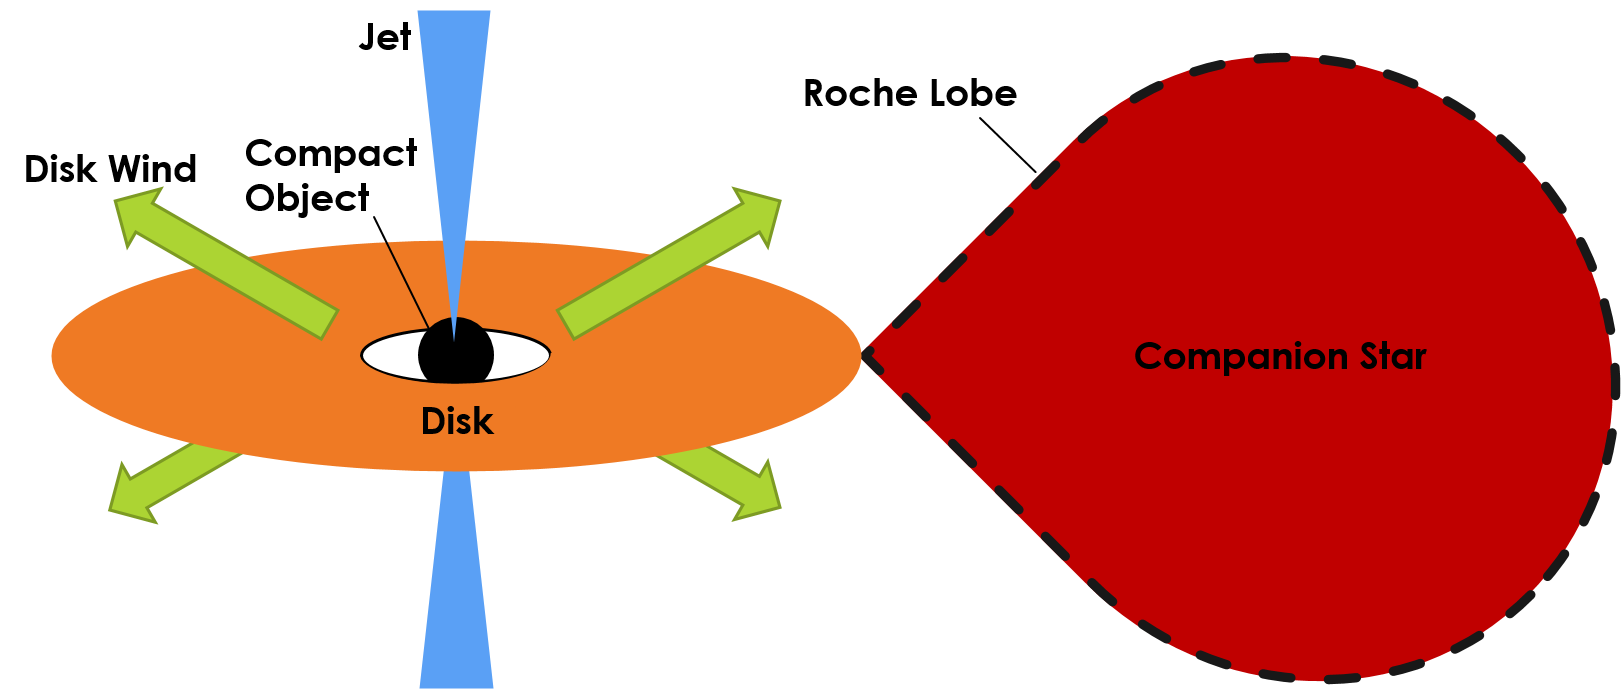
\includegraphics[width=\columnwidth, trim = 0mm 0mm 0mm 0mm]{images/xrbcartoon.eps}
    \captionsetup{singlelinecheck=off}
    \caption[A cartoon illustrating the basic geometry of a simple X-ray binary.]{A cartoon illustrating the basic geometry of a simple X-ray binary.  Not shown is the non-thermal corona of material which can be inferred from spectroscopy, as the geometry of this feature is disputed.  Diagram not to scale.}
   \label{fig:xrbcartoon}
\end{figure}

\begin{figure}
   \centering
    \includegraphics[width=0.5\columnwidth, trim = 17mm 0mm 17mm 0mm, clip]{images/jet.eps}
    \captionsetup{singlelinecheck=off}
    \caption[An 8\,GHz radio image from \citet{Stirling_Jet} showing a jet from the HMXB Cyg X-1.]{An 8\,GHz radio image from \citet{Stirling_Jet} showing a jet from the HMXB Cyg X-1 (at the origin of the image).  The lowest countour is 0.4\,mJy\,beam$^{-1}$, and other contours represent factors of 2.}
   \label{fig:jet}
\end{figure}

\par X-ray spectral studies of LMXBs find that, in addition to a black-body\footnote{The energy spectrum of a black body at temperature $T$ is given by \[F_T(\nu)=\frac{N\nu^3}{e^\frac{h\nu}{k_BT}-1}\] for some constant $N$ \citep{Planck}.  $k_B$ is the Boltzmann Constant, and $c$ is the speed of light in a vacuum.} like accretion disk, the systems must each contain a non-thermal `corona' component.  This corona emits X-rays via Compton upscattering.  In this process, photons emitted from the disk collide with energetic electrons in the corona.  The photons, on average, gain energy from these collisions and are scattered back into space; some in the direction of observers on the Earth.  This leads to a characteristic power-law\footnote{A power-law distribution is any distribution with the functional form $f(x)=cx^k$ for some constants $c$ and $k$.} energy distribution signature at high energies, which can be seen in the spectra of LMXBs.  As I show in the simulated LMXB energy spectrum in Figure \ref{fig:toyspec}, the emission from the corona tends to dominate above energies of $\sim10$\,keV.
\par Models of the geometry of the coronal region have evolved over the years.  While the corona has been historically treated as if it was a single point fixed above the centre of the disk (the so-called `Lamp Post' model, e.g. \citealp{Rozanska_Lamppost}), more recent models tend to treat it either as an optically thin\footnote{An optically thin medium is defined as a medium in which an average photon interacts $<1$ times while passing through.} flow of material onto the compact object or equate it with the base of the radio jet (e.g. \citealp{Skipper_CoronaGeo}).

\begin{figure}
   \centering
    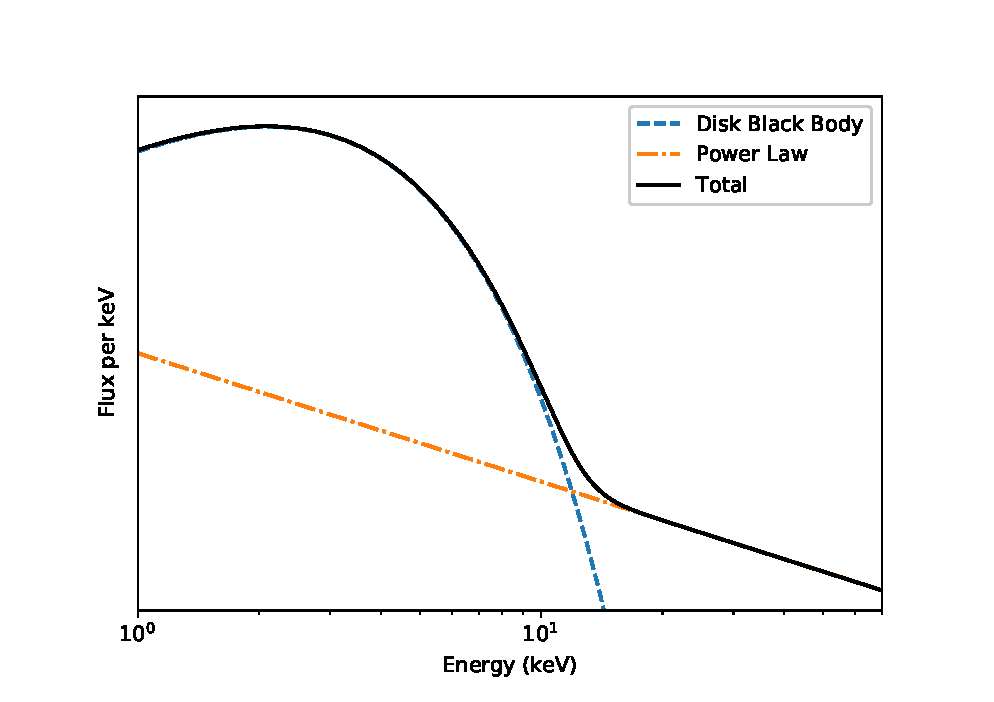
\includegraphics[width=0.7\columnwidth, trim = 10mm 0mm 10mm 10mm, clip]{images/toy_spec.eps}
    \captionsetup{singlelinecheck=off}
    \caption[A simulated, simplified spectrum of an LMXB, showing the two main components visible in X-ray: the accretion disk and the corona.]{A simulated, simplified spectrum of an LMXB, showing the two main components visible in X-ray: the accretion disk (blue) and the corona (orange).  The disk is generally modelled as a disk black body, a sum of black bodies at different temperatures corresponding to different annuli in the disk (e.g. \citealp{Mitsuda_diskbb}), while the corona is modeled as a power law.}
   \label{fig:toyspec}
\end{figure}

\par Another important component of an X-ray binary is the disk wind.  Due to the high temperatures and pressures in the inner part of the accretion disk, matter on the surface of the disk can obtain enough energy to escape the gravitational well of the compact object.  This matter is ejected from the system in large-scale, high velocity winds; studies of the spectral lines present in these winds have shown that they can have speeds approaching the speed of light (e.g. \citealp{Degenaar_BPSpec}).

\subsubsection{Neutron Star X-ray Binaries}

\label{sec:NSintro}

\par The geometry of an X-ray binary is somewhat more complicated when the compact object is a neutron star.  Unlike black holes, neutron stars are in general highly-magnetised systems, and the introduction of a large, strong magnetic field to an XRB has implications for the geometry of the accretion flow.  At some point in the inner accretion disk, it is possible that the pressure exerted by this magnetic field becomes dominant over the gas and photon pressures.  At this point, ionised material becomes `frozen-in' to the magnetic field lines, and is only able to freely move along them; due to the extreme temperatures in the inner portion of the accretion disk, the vast majority of material in this region is ionised.  The result of this effect is a disruption of the flow in the inner part of the accretion disk, in which matter is funneled along field lines and onto the poles of the neutron star.  This causes the poles of the neutron star to become extremely hot; as the neutron star spins, it appears to pulse as seen by an external observer due to the magnetic poles coming in and out of view.  These objects are referred to as accreting X-ray pulsars.
\par In addition to the effects of the magnetic field, there is another significant difference between neutron star and black hole binaries.  Black holes are surrounded by an event horizon from which no light can emerge, meaning that the compact object in black hole X-ray binaries cannot be seen directly.  Neutron stars, on the other hand, have no such event horizon.  As such the surface of the neutron star itself, and any phenomena that take place there, can also be seen.
\par One of the most spectacular events that can occur on the surface of a neutron star is a Type I X-ray burst.  These occur when matter accreted onto the surface of the neutron star reaches a critical temperature and pressure, and nuclear fusion is triggered.  This results in a flash of energy, which causes a runaway thermonuclear explosion across all or most of the neutron star surface.  Type I bursts appear in data as a sudden $\sim1$--2 orders of magnitude increase in X-ray flux, followed by an power-law decay as the neutron star surface cools.  As Type I bursts are distinctive features which require a surface on which to occur, they are often used as a diagnostic tool to identify an unknown LMXB compact object as a neutron star.

\section{Low Mass X-Ray Binary Behaviour}

\par LMXBs are not static systems, and most show complex variability over timescales of milliseconds to years.  Broadly speaking, LMXBs can be divided into persistent systems and transient systems.  Persistent systems have always observed to be bright since their discovery, implying a constantly high rate of accretion.  In some objects, this bright, high-accretion rate state has persisted for at least $\geq20$ years (e.g. GRS 1915+105, \citealp{Deegan_1915}).
\par Transient LMXBs have a somewhat more complicated life cycle.  These objects spend most of their time in a ``quiescent'' state, during which they are faint in X-rays and only a small amount of material is being accreted.  However these objects also undergo ``outbursts'', during which they increase in intensity by many orders of magnitude for a period of days to months.  The frequency of these outbursts varies widely between sources, ranging from one every month or so to one every few decades or longer.
\par LMXB outbursts tend to follow a predictable path, evolving through a number of different `states' as they progress.  I show some of these states in Figure \ref{fig:Fender} on a so-called `hardness-intensity diagram', which traces how the brightness and the spectral shape of a source evolve over time (see Section \ref{sec:hids} for more information on hardness-intensity diagrams).  At the start of a typical outburst emission from the source is spectrally hard, i.e. dominated by higher-energy photons.  This part of the outburst is referred to as a Low/Hard State (bottom-right of Figure \ref{fig:Fender}), and a radio jet is generally visible at this time.  The luminosity of the source gradually increases until it reaches some maximum, and then emission begins to become softer as the system heads towards the High/Soft State (top-right of Figure \ref{fig:Fender}).  During this transition, the system crosses the so-called `jet line', and the radio jet switches off.  Sources tend to spend a large portion of their outbursts in the high/soft state, appearing to meander in the hardness-intensity diagram.  This meandering may include additional crossings of the jet line, causing the radio jet to flicker on and off during this period.  The X-ray luminosity of the source then decreases, before the source returns to the hard state along a path of approximately constant luminosity.  The source then fades back into quiescence.  This typical outburst behaviour forms a distinctive `q' shape in the hardness-intensity diagram, as I show in Figure \ref{fig:Fender}, and can be thought of as the inner accretion disk filling with matter before draining onto the compact object or out of the system in winds (e.g. \citealp{Fender_UniJets}).  This relatively complex evolution over the course of an outburst highlights the fact that accretion is not a simple process, and that understanding accretion gives us better understanding of a areas of the physics of matter in extreme environments.

\begin{figure}
   \centering
    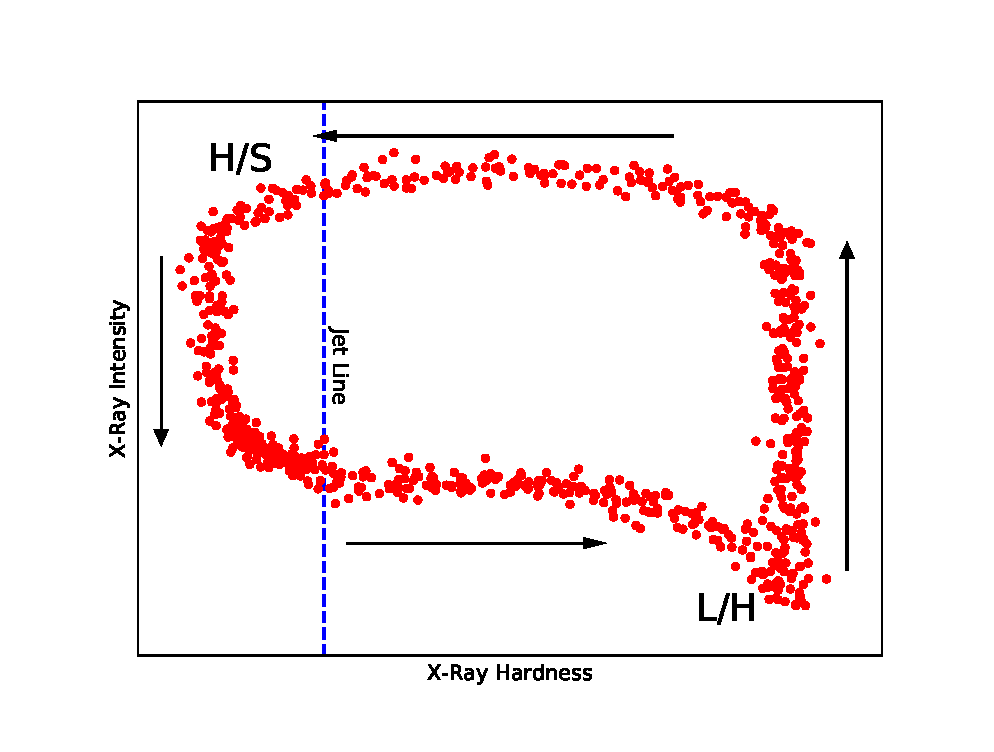
\includegraphics[width=\columnwidth, trim = 0mm 0mm 0mm 0mm, clip]{images/Fender_D.eps}
    \captionsetup{singlelinecheck=off}
    \caption[A cartoon hardness-intensity diagram adapted from \citet{Fender_UniJets}, showing the evolutionary path of a typical LMXB outburst.]{A cartoon hardness-intensity diagram adapted from \citet{Fender_UniJets}, showing the evolutionary path of a typical LMXB outburst and roughly indicating the positions of the Low/Hard (L/H) and High/Soft (H/S) States.  The jet line roughly demarcates the portion of the outburst in which a jet is observed (right of the line) from the portion in which it is not observed (left of the line).}
   \label{fig:Fender}
\end{figure}

\section{Relativistic Effects}

\par One of the most obvious extreme physical environments that accretion physics sheds light on is, of course, extreme gravitational fields.  General relativistic effects around compact objects are often expressed in relation to the gravitational radius $r_g$, defined as:

\begin{equation}
r_g=\frac{2GM}{c^2}
\end{equation}

Where $G$ is the gravitational constant, $c$ is the speed of light and $M$ is the mass of the compact object.  1$r_g$ is equal to the Schwarzchild radius, or the radius of the event horizon of a non-rotating black hole with mass $M$ \citep{Schwarzschild}.
\par One result of general relativity which is important when considering compact object accretion disks is the accretion of an Innermost Stable Circular Orbit, or ISCO.  This radius is at $3r_g$ from the centre of a non-rotating object, placing it well outside the event horizon of a black hole and above the surface of some neutron stars.  It can be shown that any isolated point mass crossing this boundary from the outside will continue into the black hole, whereas any point mass crossing it from the inside will continue to infinity; as such, no stable orbit can exist with a periastrion smaller than this radius. It can be shown that an accretion disk is also bounded by this radius \citep{Kozlowski_ISCO}, meaning that XRB accretion disks must all have an inner truncation radius at at least $3r_g$ from the compact object.  Within this radius, matter falls directly onto the compact object.
\par In general, a black hole can be described in 3 parameters\footnote{This conjecture is often referred to as the `No-Hair' theorem.}: in addition to mass, a black hole can possess non-zero angular momentum (or spin) and charge.  As the precursor stars to black holes are neutrally charged, it is expected that all astrophysical black holes are very close to being neutral as well.  However, these precursor stars also possess non-zero angular momentum.  As such, it is expected that most if not all astrophysical black holes are spinning.  This spin is generally expressed as a number between 0 and 1, where 0 denotes a non-rotating black hole and 1 is the maximum permitted angular momentum the object can possess.
\par General relativity tells us that this spin will also have a significant effect on accretion physics.  First of all, this spin serves to change the position of the ISCO; moving it to a maximum of $4.5r_g$ for a black hole with spin of 1.  A spinning black hole also distorts the space time around it, in a process known as frame-dragging.  This forces matter close to the black hole to orbit in the same plane as it.  As there is no reason to assume the outer disk orbits in the same plane as the black hole, this can lead to situations in which the accretion disk is warped, which in turn has implications for the flow of matter within it.
\par It is clear that the general relativity should have observable implications on the flow of matter onto the accretion disk.  Studying the physics of accretion therefore allows us to measure parameters such as the spin of black holes that would otherwise be inaccessible to us.  Additionally, a full understanding of the accretion onto the compact objects would allow us to look for discrepancies between what is observed and what is expected from relativity.  Therefore, a full understanding of accretion is one route to testing the theory of relativity itself under some of the most extreme conditions in the universe.

\cleardoublepage

\chapter{The Physics of Accretion}

\label{sec:PhysAcc}

\section{The Eddington Limit}

\par Consider an element of gas at distance $r$ from a compact object, with mass $m$.  This element of gas is acted on by a inwards-pointing gravitational force given by:
\begin{equation}
F_G=\frac{GMm}{r^2}
\end{equation}
Where $M$ is the mass of the compact object.
\par The X-ray Binary is of course bright in electromagnetic radiation, emitting a luminosity $L$.  If we assume that this luminosity is emitted isotropically, then the electromagnetic flux at distance $r$ is given by:
\begin{equation}
\phi(r)=\frac{L}{4\pi r^2}
\end{equation}
Electromagnetic radiation exerts a pressure on material corresponding to $\phi/c$.  As such, the radiation from the X-ray binary exerts an outwards force on our gas element corresponding to:
\begin{equation}
F_L=\frac{\kappa m\phi(r)}{c}=\frac{L\kappa m}{4\pi r^2c}
\end{equation}
Where $\kappa$ is the opacity of the cloud, or its surface area per unit mass.
\par If $F_G$ and $F_L$ are equal, then no net force is exerted on our cloud of matter and it will not accrete onto the compact object.  This happens when:
\begin{eqnarray}
F_G&=&F_L\\ \nonumber \\
\frac{GMm}{r^2}&=&\frac{L\kappa m}{4\pi r^2c} \\ \nonumber \\
L&=&\frac{GMm}{r^2}\frac{4\pi r^2c}{\kappa m} \\ \nonumber \\
L&=&\frac{4\pi GMc}{\kappa}
\end{eqnarray}
This luminosity, denoted as $L_E$, is the Eddington luminosity of the source; the maximum luminosity an object can be and still have accretion take place.  It only depends on the mass of the compact object $M$ and the opacity of the accreting material $\kappa$, which in turn depends on the chemical make-up of the accretion disk.  As accretion disks tend to be dominated by ionised hydrogen, $\kappa$ is usually assumed to be $\sigma_T/m_p$, where $\sigma_T$ is the Thomson scattering cross section of an electron and $m_p$ is the mass of a proton.  This assumption yields the final formula which only depends on the mass of the compact object:
\begin{equation}
L_E=\frac{4\pi GMm_pc}{\sigma_T}
\end{equation}
The luminosity due to matter falling into a black hole can be expressed as:
\begin{equation}
L=\eta\dot{M}c^2
\end{equation}
Where $\dot{M}$ is the accretion rate and $\eta$ is the efficiency at which infalling matter is converted to outgoing radiation.  As such, $L_E$ also corresponds to a theoretical maximum accretion rate.
\par However, a number of X-ray binaries have been seen to shine at luminosities above this limit; in one of the most extreme cases, the confirmed neutron star XRB M82 X-1 has a luminosity of $\sim100L_E$ \citep{Bachetti_M82X1}.  This is possible due to the fact that a number of assumptions made when calculating the Eddington limit do not apply to physical XRBs.  In particular, the calculation performed above assumes that both accretion on to the compact object, as well as electromagnetic emission from it, are isotropic.  An object which appears to exceed the Eddington limit may do so if it is not isotropically accreting, which is the case for XRBs as these systems accrete from near-planar disks.  A system may further exceed the Eddington limit if its emission is beamed; an XRB beamed in the direction of the Earth would lead us to infer an artificially high value of $L$, and thus overestimate its luminosity with respect to the Eddington Limit.
\par Despite these setbacks, the Eddington Luminosity is a useful tool to compare XRBs with different compact object masses.  By expressing the luminosity of an object as a fraction of its Eddington Limit, often referred to as its Eddington fraction, objects can be rescaled in such a way that we can compare how dominant photon pressure must be in each accretion disk.

\section{The Propellor Effect}

\par Another limit on accretion rate arises when one considers the effect of a strong neutron star magnetic field.  To understand this effect, we must first define two characteristic radii of such a system.
\par First, assume that the magnetic field of the neutron star can be approximated as a set of rigid field lines which are anchored to points on the neutron star surface.  The magnetic field can then be thought of as a `cage' which rotates with the neutron star at its centre.  The straight-line speed of a point on this rotating cage is given by:
\begin{equation}
v_\nu(r)=2\pi r\nu
\end{equation}
Where $r$ is the distance from the neutron star centre and $\nu$ is the rotation frequency of the neutron star.  This can be compared with the Keplerian speed, or the speed of a particle in a Keplerian orbit around the compact object.  This is given by:
\begin{equation}
v_K(r)=\sqrt{\frac{GM}{r}}
\end{equation}
Where $M$ is the mass of the neutron star.  By setting these equal, we can find the radius at which the magnetic field is rotating at the same speed as a particle in a Keplerian orbit:
\begin{eqnarray}
v_\nu(r)&=&v_K(r)\\ \nonumber \\
2\pi r\nu&=&\sqrt{\frac{GM}{r}}\\ \nonumber \\
r^3&=&\frac{GM}{4\pi^2\nu^2}\\ \nonumber \\
r&=&\sqrt[3]{\frac{GM}{4\pi^2\nu^2}}
\end{eqnarray}
This radius is denoted as $r_c$, the co-rotation radius.  Inside of this radius, an particle in an equatorial Keplerian orbit has a greater velocity than the magnetic field lines; outside this radius, the magnetic field lines are moving faster.  To understand the significance of this radius, we must define another characteristic radius of the system.
\par In a neutron star accretion disk, there are three significant sources of pressure: gas (or ram) pressure $P_g$, photon pressure $P_\gamma$ and magnetic pressure $P_\mu$.  Whichever pressure is dominant in a given location will govern the physics of matter in that region.
\par Photon pressure falls off sharply outwards from the inner disk, so I will assume it is negligible in the region of the disk considered here.  Assuming that the field of the neutron star is a dipole, the magnetic pressure at its equator can be given as:
\begin{eqnarray}
P_\mu&=&\frac{B^2}{2\mu_0}\\ \nonumber \\
B(r)&=&B_0\left(\frac{R_{NS}}{r}\right)^3\label{eq:NS}\\ \nonumber \\
\therefore\quad P_\mu&=&\frac{B_0^2}{2\mu_0}\left(\frac{R_{NS}}{r}\right)^6
\end{eqnarray}
Where $\mu_0$ is the vacuum permeability, $B_0$ is the equatorial magnetic field strength at the neutron star surface, $R_{NS}$ is the radius of the neutron star and Equation \ref{eq:NS} is the equation for the magnetic field strength above the equator of a dipole.
\par The functional form of the ram pressure depends on the assumed accretion geometry of the system.  As I did when calculating the Eddington, I will assume the simplest possible case of spherically accreting free-falling matter.  The ram pressure is then given by:
\begin{equation}
P_g=\frac{\dot{M}}{4\pi r^2}\sqrt{\frac{2GM}{r}}
\end{equation}
When $P_\mu>P_g$, accreting material is dominated by magnetic pressure in such a way that material is `frozen' onto magnetic field lines \citep{Alfven_Waves}; this results in material flowing onto the neutron star surface along magnetic field lines onto the poles, as described in section \ref{sec:NSintro}.  It is possible to express the region of the accretion disk within which matter is magnetically dominated:
\begin{eqnarray}
P_g&<&P_\mu\\ \nonumber \\
\frac{\dot{M}}{4\pi r^2}\sqrt{\frac{2GM}{r}}&<&\frac{B_0^2}{2\mu_0}\left(\frac{R_{NS}}{r}\right)^6\\ \nonumber \\
\frac{GM\dot{M}^2}{8\pi^2 r^5}&<&\frac{B_0^4}{4\mu_0^2}\left(\frac{R_{NS}}{r}\right)^{12}\\ \nonumber \\
r^7&<&\frac{2\pi^2}{G\mu_0^2}\frac{B_0^4R_{NS}^{12}}{M\dot{M}^2}\\ \nonumber \\
r&<&\sqrt[7]{\frac{2\pi^2}{G\mu_0^2}\frac{B_0^4R_{NS}^{12}}{M\dot{M}^2}}
\end{eqnarray}
This radius, the magnetospheric or Alfv\'en radius, is denoted as $r_\mu$.
\par Now it is possible to consider what happens to matter approaching $r_\mu$ in two different physical regimes.  First of all, consider a system in which $r_c>r_\mu$.  In this case, magnetic field lines at $r_\mu$ are moving slower than the Keplerian speed.  An element of matter approaching this radius from a Keplerian orbit will experience a torque slowing it down as it freezes onto the field lines.  By Kepler's laws of planetary motion, this necessarily decreases the altitude of this element of matter.  This pulls the element further into the magnetically-dominated regime and allows it to accrete freely along the field line onto the neutron star.
\par Now consider what happens when $r_c<r_\mu$.  In this case, field lines at $r_\mu$ are moving faster than Keplerian speed.  An element of matter approaching $r_\mu$ will therefore experience a torque speeding it up as it becomes frozen onto magnetic field lines.  This will increase its altitude, driving it back away from $r_\mu$.  In this case, the magnetospheric radius acts as a barrier to infalling matter, repelling any gas that approaches it and stopping accretion onto the neutron star surface.  This set of circumstances is known as the `propellor regime', due to the rapidly rotating field lines acting like a `propellor' which blow the inner part of the disk away.
\par As the propellor regime is expected to occur for $r_c<r_\mu$, it is possible to work out what kind of system this should be observed in:
\begin{eqnarray}
r_c&<&r_\mu\\ \nonumber \\
\left(\frac{GM}{4\pi^2\nu^2}\right)^{1/3}&<&\left(\frac{2\pi^2}{G\mu_0^2}\frac{B_0^4R_{NS}^{12}}{M\dot{M}^2}\right)^{1/7}\\ \nonumber \\
M^{10/21}\dot{M}^{2/7}&<&k\nu^{2/3}B_0^{4/7}R_{NS}^{12/7}
\end{eqnarray}
Where $k$ is a constant.  Assuming that the radius and mass of neutron stars does not vary much, this inequality tells us that the propellor regime is more likely to be observed in neutron star XRBs with a high spin frequency and a high magnetic field.  It also tells us that the propellor effect places a \textit{lower} limit on accretion in such systems: accretion is not possible unless infalling matter can apply enough ram pressure to push the magnetospheric radius inside the corotation radius.
\par There are numerous problems with this relatively simplistic view of accretion in a highly magnetic regime.  Much as in our calculation of the Eddington Limit, it is not clear that all the assumptions are physical.  This calculation again depends on an unphysical spherical accretion geometry, and makes the assumption that the magnetic field lines can in no way be warped by the movement of ionised matter on them.  Additionally \citet{White_MRad} show that the magnetospheric radius calculated for neutron stars may fall close enough to the inner edge of the disk that photon pressure cannot be safely ignored.  In this scenario, calculating the magnetospheric radius becomes much less straightforward.
\par Despite these problems, an effect observationally similar to the propellor effect is observed in a number of astrophysical neutron star XRBs. xxxxx

\section{The Shakura-Sunyaev Disk Model}

\par To understand how the very non-spherical nature of accretion disks affects their physics, it is important to construct models.  Much of our understanding of the physics of astrophysical accretion disks stems from a model proposed by Nikolai Shakura and Rashid Sunyaev in 1973 \citep{Shakura_Disk}.  This model specifically considered the effects of accretion onto a black hole.  By showing that this would result in a system which would be bright in the X-ray, and describing how such a system would appear, this model proved pivotal in the community's acceptance of the earliest XRB identifications (e.g.\citealp{Bolton_CygX1}).
\par \citet{Shakura_Disk} model the accretion disk as a structure held up by centrifugal forces, generated by the large amount of angular momentum possessed by infalling matter due to the orbit of the binary system.  Frictional forces cause this angular momentum to be transferred outwards, heating up the disk and allowing matter to fall in towards the black hole.  The efficiency with which this angular momentum is transferred, parameterised as $\alpha$, can then be thought of as a measure of the viscosity of the disk.
\par \citet{Shakura_Disk} their calculations on Newtonian mechanics; as such they ignore they ignore the region of the disk for $r<3r_g$, or the ISCO, where relativistic effects become important.  They also assume that the disk in a steady state, that it is geometrically thin (such that height of the disk $H\ll r$ everywhere) and that it is cylindrically symmetric.  The last two assumptions allow us to write down formulae for the surface density $\Sigma$, radial velocity $u_r$ and accretion rate $\dot{M}$ of the disk as a functions of radius $r$:
\begin{eqnarray}
\Sigma(r)&=&\int_{-H}^H\rho(r,z) dz\label{eq:base1}\\\nonumber \\
u_r(r)&=&\frac{1}{\Sigma(r)}\int_{-H}^H\rho(r,z)v_r(r,z)dz\label{eq:base2}\\\nonumber \\
\dot{M}(r)&=&-2\pi r\Sigma(r) u_r(r)\label{eq:base3}
\end{eqnarray}
Where $\rho(r,z)$ is the density at a radius $r$ and height $z$, and $v_r$ is the radial velocity of the gas at this point.
\par Now consider the Euler equations of hydrodynamics:
\begin{eqnarray}
\frac{\partial\rho}{dt}+\dv(\rho\bm{v})&=&0\label{eq:consmass}\\\nonumber \\
\rho\left(\frac{\partial\bm{v}}{dt}+(\bm{v}\cdot\dv) \bm{v}\right)&=&-\dv p\label{eq:fma}
\end{eqnarray}
Where Equation \ref{eq:consmass} is the conservation of mass and Equation \ref{eq:fma} is a differential form of Newton's second law of motion.  These equations can be cast in cylindrical co-ordinates to give 4 equations: the recast continuity equation and one motion equation for each of the radial ($r$), vertical ($z$) and azimuthal ($\theta$) directions:
\begin{eqnarray}
\frac{\partial\rho}{\partial t}+\frac{1}{r}\frac{\partial(r\rho v_r)}{\partial r}+\frac{1}{r}\frac{\partial v_\theta}{\partial\theta}+\frac{\partial v_z}{\partial z}&=&0\label{eq:ssc}\\\nonumber\\
\rho\left(\frac{\partial v_r}{\partial t}+v_r\frac{\partial v_r}{\partial r}+\frac{v_\theta}{r}\frac{\partial v_r}{\partial\theta}+v_z\frac{\partial v_r}{\partial z}-\frac{v_\theta^2}{r}\right)&=&\frac{-\partial p}{\partial r}\label{eq:ssr}\\\nonumber\\
\rho\left(\frac{\partial v_\theta}{\partial t}+v_r\frac{\partial v_\theta}{\partial r}+\frac{v_\theta}{r}\frac{\partial v_\theta}{\partial\theta}+v_z\frac{\partial v_\theta}{\partial z}+\frac{v_rv_\theta}{r}\right)&=&\frac{-\partial p}{\partial\theta}\\\nonumber\\
\rho\left(\frac{\partial v_z}{\partial t}+v_r\frac{\partial v_z}{\partial r}+\frac{v_\theta}{r}\frac{\partial v_z}{\partial\theta}+v_z\frac{\partial v_z}{\partial z}\right)&=&\frac{-\partial p}{\partial z}\label{eq:ssz}
\end{eqnarray}
By the assumptions that the disk is in a steady state and cylindrically symmetric, we can set all $\frac{\partial}{\partial\theta}$ and $\frac{\partial}{\partial t}$ terms to zero, simplifying equations \ref{eq:ssr} to \ref{eq:ssz}:
\begin{eqnarray}
\rho\left(v_r\frac{\partial v_r}{\partial r}+v_z\frac{\partial v_r}{\partial z}-\frac{v_\theta^2}{r}\right)&=&\frac{-\partial p}{\partial r}\label{eq:ssrs}\\\nonumber\\
\rho\left(v_r\frac{\partial v_\theta}{\partial r}+v_z\frac{\partial v_\theta}{\partial z}+\frac{v_rv_\theta}{r}\right)&=&0\label{eq:ssts}\\\nonumber\\
\rho\left(v_r\frac{\partial v_z}{\partial r}+v_z\frac{\partial v_z}{\partial z}\right)&=&\frac{-\partial p}{\partial z}\label{eq:sszs}
\end{eqnarray}
We can average the density term on left-hand side of Equation \label{eq:ssc} in the $z$-direction, and substitute in the results from Equations \ref{eq:base1} to \ref{eq:base3} to find:
\begin{eqnarray}
\frac{1}{r}\frac{d}{dr}\left(r\int_{-H}^H\rho v_rdz\right)&=&0\\\nonumber\\
\frac{1}{r}\frac{d(r\Sigma u_r)}{dr}&=&0\\\nonumber\\
\frac{-1}{2\pi r}\frac{d\dot{M}}{dr}&=&0
\end{eqnarray}
Therefore the rate of inwards matter flow $\dot{M}$ is constant at all $r$.
\par Using the fact that the angular velocity $\omega$ of an element in the gas can be written as $\omega=v_\theta/r$, we can re-write Equation \ref{eq:ssrs} as:
\begin{equation}
\rho\left(v_r\frac{\partial v_r}{\partial r}-\omega^2r\right)=-\frac{\partial p}{\partial r}-\rho v_z\frac{\partial v_r}{\partial z}
\end{equation}
We can rewrite $v_z\frac{\partial v_r}{\partial z}$ as $\frac{\partial v_r}{\partial z}\frac{\partial z}{\partial t}$, which is equal to the inwards acceleration of a gas element moving in the $z$-direction.  As the disk is assumed to be in a cylindrically symmetric gravitational potential, this acceleration can be given by $\dot{v}_r=\frac{GM}{r^2}$.  This leads to:
\begin{eqnarray}
\rho\left(v_r\frac{\partial v_r}{\partial r}-\omega^2r\right)&=&-\frac{\partial p}{\partial r}-\rho\frac{GM}{r^2}\\\nonumber\\
\rho\left(v_r\frac{\partial v_r}{\partial r}-\omega^2r\right)&=&-\frac{\partial p}{\partial r}-\rho\omega_k^2r
\end{eqnarray}
Assuming that is thin and angular momentum is only transferred slowly, i.e. $v_r\frac{\partial v_r}{\partial r}\ll\omega$, this leads to:
\begin{equation}
\omega\approx\omega_k
\end{equation}
Showing that gas elements in the disk orbit at Keplerian speeds.
\par Using similar logic, Equation \ref{eq:sszs} becomes:
\begin{equation}
\rho\omega_k^2 z=\frac{-\partial p}{\partial z}\label{eq:idgas}
\end{equation}
The ideal gas law $p=\rho RT$\footnote{$R$ is the specific gas constant, equal to the Boltzmann Constant $k_B$ divided by the mean molar mass of the gas.} can then be used to rewrite equation \ref{eq:idgas}:
\begin{equation}
\frac{p}{RT}\omega_k^2 z=\frac{-\partial p}{\partial z}\label{eq:idgas2}
\end{equation}
If we assume that the disk is chemically homogeneous and isothermal in the $z$-direction, then neither $R$ nor $T$ depend on $z$.  Equation \ref{eq:idgas2} then admits the solution:
\begin{equation}
\rho=\rho_0(r)e^{\left(\frac{-z^2\omega_k^2}{2RT}\right)}=\rho_0(r)e^{\frac{-z^2}{2H^2}}
\end{equation}
Where $\rho_0$ is the density at radius $r$ when $z=0$.  As such, the density of the disk has a Gaussian profile in the $z$-direction, with a scale-width $H_s$ given by:
\begin{equation}
H_s=\frac{\sqrt{RT}}{\omega_k}
\end{equation}
This shows that the scale height of the disk is finite for all $r$.  As the integral between $-\infty$ and $+\infty$ of a Gaussian with a finite scale-width is finite, the disk contains a finite amount of matter.
\par Finally, we can look at the solutions to Equation \ref{eq:ssts}.  As every term in this equation depends on either $v_\theta$ or a derivative thereof, this equation admits the solutions $\rho=0$ or $v_\theta=0$.  Both of these solutions imply accretion rates of zero, as any matter in the disk must have a non-zero density and angular momentum.  In order to resolve this problem, \citet{Shakura_Disk} add the divergence of the viscous stress tensor \citep{Landau_Tensor} to the right-hand side of Equation \ref{eq:ssts} to represent the effects of viscosity within the disk.  By doing this, they find the following two results:
\begin{eqnarray}
\dot{M}&=&\frac{4\pi H\eta_b r}{\omega}\frac{\partial\omega}{\partial r}\label{eq:diffrot}\\\nonumber\\
\dot{M}&=&6\pi\eta_b H\label{eq:viscos}
\end{eqnarray}
Equation \ref{eq:diffrot} confirms that the disk is a differential rotator, while Equation \ref{eq:viscos} confirms that accretion can only take place when $\eta_b$ (the bulk viscocity) is non-zero.
\par \citet{Shakura_Disk} found that molecular viscosity alone cannot be high enough to result in the high values of $\dot{M}$ inferred for observed XRBs.  Instead, the authors assume that turbulence is present in the disk.  Using formulae pertaining to turbulent hydrodynamics, and by ignoring supersonic perturbations, they find an upper bound on bulk viscosity $\eta$:
\begin{equation}
\eta_b\leq\frac{2}{3}\rho_0H\sqrt{RT}
\end{equation}
As such, they define their dimensionless viscosity parameter $\alpha$ as:
\begin{equation}
\alpha\equiv\frac{3\eta_b}{2\rho_0H\sqrt{RT}}\quad\quad\quad\alpha\leq1
\end{equation}

\subsection{The source of Turbulence}

\par \citet{Shakura_Disk} do not answer the question of what physical process causes the turbulence required to stabilise accretion disks.  \citet{Balbus_MRI} were among the first to propose the Magnetorotational Instability \citep[MRI,][]{Velikhov_MRI,Chandrasekhar_MRI} as the source of this turbulence.  MRI is a process which occurs in an ionised and differentially rotating disk.  Fluctuations in the material in the disk generate internal magnetic fields.  The field lines associated with these fields, in general, extend a finite distance in the radial direction, thus connecting gas elements at different radii.  As gas elements in a Shakura-Sunyaev accretion disk orbit the compact object at Keplerian speeds, elements of gas at different radii move at different orbital speeds.  As such, these internal magnetic field lines become stretched as gas orbits the compact object.  This field line stretching imparts a torque on the gas elements, causing the outer, slower element to speed up and the inner, faster element to slow down.  As such, the net result of this process is an outwards transfer of angular momentum.
\par \citet{Balbus_MRI} found that the angular momentum transfer due to MRI was more significant than that due to friction, hydrodynamic turbulence or other sources in an accretion disks.  They suggest therefore that MRI is the main component of outwards angular momentum transfer, and thus of $\alpha$, in astrophysical accretion disks.

\section{Disk Instabilities}

\par A number of additional effects can be observed in the accretion disks of systems near or above the Eddington limit. xxxxx

\label{sec:diskinstab}

L-E xxxxx Using the assumptions present in the thin disk models of \citealp{Shakura_Disk} and \citealp{Novikov_Torque}, \citealp{Lightman_Instability} show that an annulus within a thin, radiatively dominated disk has an effective negative radial diffusion coefficient.  As such, any initially smooth disk under these conditions tends to separate into dense annuli.

\section{GRS 1915+105 and IGR J17091-3624}

\par One famous system in which disk instabilities are extremely apparent is the black hole LMXB GRS 1915+105.  GRS 1915+105 \citep{CastroTirado_GRS1915}, hereafter GRS 1915, is a black hole LMXB which accretes at between a few tens and 100\% of its Eddington Limit (e.g. \citealp{Vilhu_SupEd,Done_GRS_HighAcc,Fender_DiskJet}).  The system lies at a distance of $8.6\pm2.0$\,kpc \citep{Reid_Parallax}, and consists of a 12.4$\pm$2.0\,M$_\odot$ black hole and a $<1$\,M$_\odot$ K-class giant star \citep{Reid_Parallax,Ziolkowski_GRSDonor}.
\par GRS 1915 has been in outburst since its discovery in 1992 \citep{CastroTirado_GRS1915}.  The extreme length of the ongoing outburst is believed to be related to the large size of its accretion disk: the components of GRS 1915 have the longest known orbital period of any LMXB \citep{Greiner_BigDisk}, in turn implying that this system has the greatest separation and the largest accretion disk.
\par GRS 1915 is also notable for the incredible variety and complexity of variability classes it exhibits (e.g. \citealp{Yadav_GRSBursts,Belloni_GRS_MI}).  In total, 15 distinct variability classes have been described \citep{Belloni_GRS_MI,KleinWolt_OmegaClass,Hannikainen_NewClass, Pahari_NewClass}, a number of which we show lightcurves of in Figure \ref{fig:GRSsample}.  The system tends to stay in one variability class for no more than a few days but similar patterns are often repeated many months or years later, suggesting some capacity of the system to `remember' which variability classes it can occupy.  Accounting for this incredible range of repeatable behaviour could be key to our understanding of radiation-dominated accretion regimes.

\begin{figure}
  \centering
  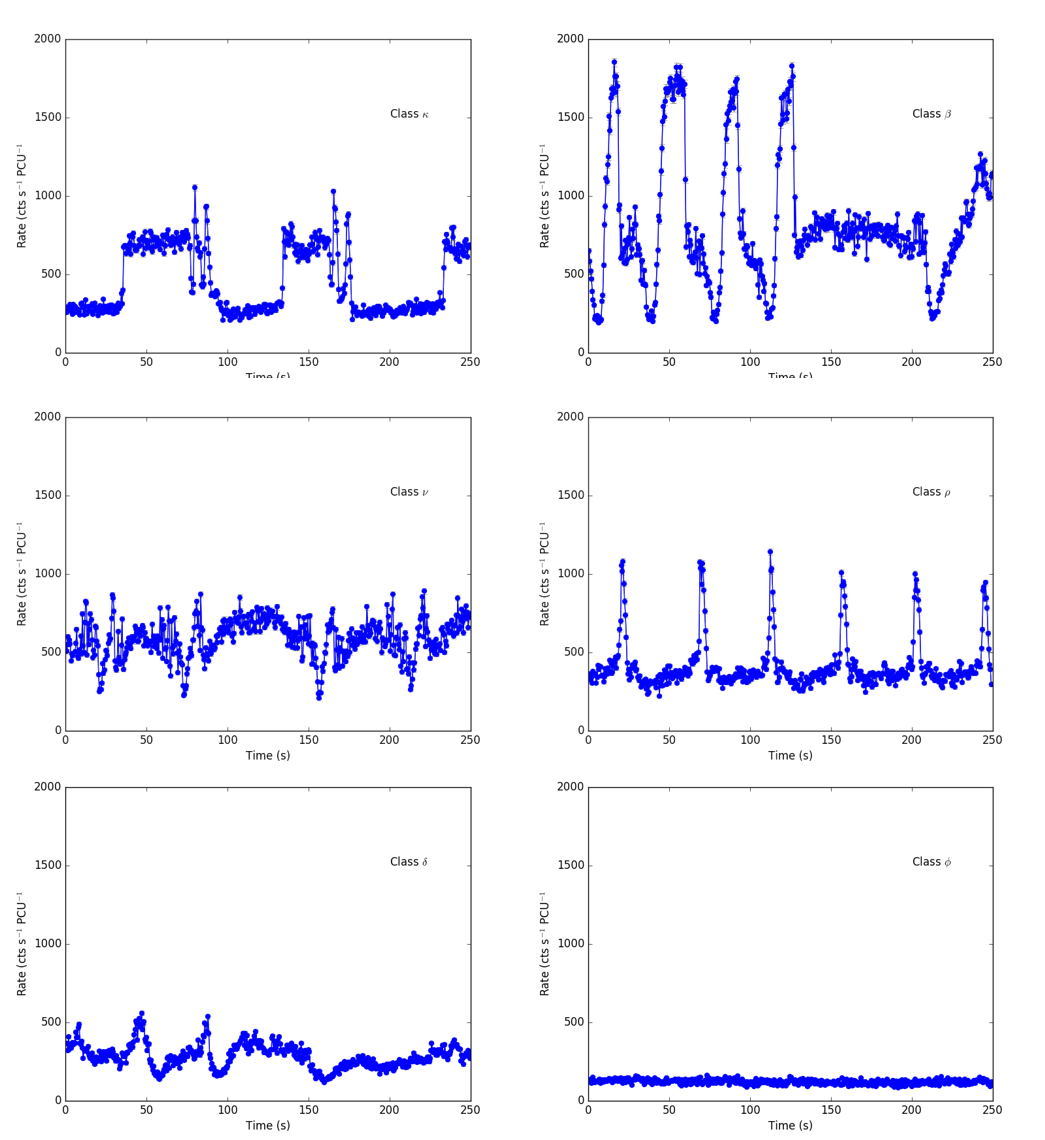
\includegraphics[width=.9\linewidth, trim= 25mm 0mm 0mm 0mm]{images/GRSsample.png}
  \caption{\small Typical lightcurves of a selection of variability classes seen in GRS 1915, taken by the PCA instrument aboard \rxte .  The classes are labelled according to the Greek letter names assigned to them in \citet{Belloni_GRS_MI}.}
  \label{fig:GRSsample}
\end{figure}

\par The variability classes of GRS 1915 consist of a number of different types of variability, with a range of amplitudes and timescales.  Variability classes in GRS 1915 are usually denoted by the Greek letter names assigned to them by \citet{Belloni_GRS_MI}.  In general the variability associated with these classes takes the form of complex patterns of flares and dips, and it occurs over timescales of 10s to 100s of seconds.  In some classes, the variability is somewhat regular.  The $\rho$ class, also referred to as the `heartbeat' class due to the similarity of its lightcurve to the output of an electrocardiagram, consists of sharp quasiperiodic flares with a recurrence time of a few tens of seconds (Middle-right panel of Figure \ref{fig:GRSsample}).  Other classes, such as class $\kappa$ shown in the top-left panel of Figure \ref{fig:GRSsample}, consist of quasiperiodic fluctuations between two quasistable count rates: in the case of class $\kappa$, there is also a period of highly structured sub-second variability at each transition between these two classes.  Finally, two classes ($\chi$ and $\phi$, an example of the latter is shown in the bottom-right panel of Figure \ref{fig:GRSsample}) show no significant variability other than red noise; these classes are separated based on their spectral properties.  It has been suggested they they may be equivalent to the hard state seen in other outbursting LMXBs \citep{VanOers_GRSHard}, providing a possible link between the behaviour of GRS 1915 and the behaviour of more typical LMXBs.
\par The dramatic variability seen in GRS 1915 was long thought to be unique, driven either by its unusually high accretion rate or by its unusually large accretion disk.  However in 2011, \citet{Altamirano_IGR_FH} identified GRS 1915-like variability in a second object: the black hole LMXB IGR J17091-3624. xxxxx



\subsection{A History of Models of GRS 1915-like Variability}

\par Over the years, a number of models and physical scenarios have been suggested to explain the complex variability seen in GRS 1915-like systems.  Successful models must also be able to explain why this type of variability is not seen in a wider array of sources.
\par One of the most best-studied classes of GRS 1915-like variability is Class $\rho$, the `heartbeat' class.  This variability class is present in both GRS 1915 and IGR J17091 (e.g. \citealp{Altamirano_IGR_FH}), and has been the focus of many of the models proposed to explain GRS 1915-like variability.  It has been shown that hard X-ray photons lag soft X-ray photons in this class (e.g. \citealp{Janiuk_Lag,Massaro_Lag}).  Other classes in GRS 1915 which show quasi-periodic flaring behaviour also exhibit this phase lag.
\par Previous authors have established models to explain both the hard photon lag as well as the `heartbeat'-like flaring itself, generally based on the instability in a radiation-dominated disk first reported by \citealp{Lightman_Instability} (see Section \ref{sec:diskinstab}).
\par \citealp{Belloni_Model1} first proposed an empirical model for flaring in GRS 1915.  They suggested that this behaviour is due to a rapid emptying of a portion of the inner accretion disk, followed by a slower refilling of this region over a viscous timescale.  These authors divided data from a given observation into equal-sized 2-Dimensional bins in count rate-colour space.  A spectral model was then fit to each of these bins independently to perform `pseudo'-phase-resolved spectroscopy (compare with the method outlined in Section \ref{sec:phasresspec}).  They showed that the quiescent time between flaring events correlates with the maximum inner disk radius during the flare; i.e., a correlation between the amount of the disk which is emptied and the time needed to refill it.  They go on to suggest that their model is able to explain all flaring-type events seen in GRS 1915.
\par The scenario proposed by \citealp{Belloni_Model1} was mathematically formalised by \citealp{Nayakshin_GRSModel}, who found that it was not consistent with a `slim' accretion disk \citep{Abramowicz_Slim} or with a disk in which viscosity $\alpha$ is constant with respect to radius.  As such, their model consists of a cold accretion disk with a modified viscosity law, a non-thermal electron corona and a transient jet of discrete plasma emissions which are ejected when the bolometric luminosity approaches the Eddington Limit.  Using this model, \citealp{Nayakshin_GRSModel} found that some formulations of $\alpha(r)$ result in the disk oscillating between two quasi-stable branches in viscosity-temperature space, over timescales consistent with those seen in the flaring of GRS 1915; they found that this occurs for accretion rates greater than 26\% of the Eddington limit.  They also found that by varying the functional form of $\alpha(r)$, their model gives rise to a number of lightcurve morphologies which generally match what is seen in data from GRS 1915.  \citealp{Janiuk_RadInstab} built on this model further by including the effect of the transient jet in cooling the disk; an effect not considered in the model by \citealp{Nayakshin_GRSModel}.  In this formulation, \citealp{Janiuk_RadInstab} found that GRS 1915-like variability should occur at luminosities as low as 16\% of Eddington.
\par \citealp{Belloni_GRS_MI} found that variability in GRS 1915 can be described by transitions between three phenomenological states, which differ in luminosity and hardness ratio.  This phenomenological scenario is at odds with the model of \citealp{Nayakshin_GRSModel}, which only results in two quasi-stable states.
\par \citealp{Nobili_Hotspot} tried to account for the hard X-Ray lag by supposing that a significant proportion of the X-Ray variability from the accretion disk comes from a single hotspot.  They suggest that the lag corresponds to a light travel time, after which a portion of this emission is Comptonised by the jet.  In this case, the geometric location of this hotspot determines the magnitude of this lag, and whether it is positive or negative.  This scenario goes some way to explaining why GRS 1915 is special, as it requires the presence of a jet during a soft-like state.
\par \citealp{Tagger_MagneticFlood} propose a magnetic explanation for the ejection of the inner accretion disk required by \citealp{Nayakshin_GRSModel} and \citealp{Janiuk_RadInstab}.  They suggest a limit cycle in which a poloidal magnetic field is advected towards the inner disk during the refilling of this region.  This field is then destroyed in reconnection events, releasing energy which results in the expulsion of matter from the inner disk.  They suggest that the three quasi-stable states proposed by \citealp{Belloni_GRS_MI} can be explained as states in the inner accretion disk with different values of plasma $\beta$.
\par \citealp{Janiuk_Lag} attempt to explain the hard lag in the heartbeats of GRS 1915 more simply, by proposing that it is caused by the non-thermal corona smoothly adjusting to changes in luminosity from the disk.  They base the variability of the disk on the model of \citealp{Nayakshin_GRSModel}, and show that the presence of a non-thermal corona which reacts to this variability naturally reproduces the lag behaviour seen in Class $\rho$ in GRS 1915.
\par \citealp{Merloni_MagDom} also propose a magnetic explanation for the reformulation of $\alpha(r)$ required by the model of \citealp{Nayakshin_GRSModel}.  Assuming that the viscosity in the accretion disk is dominated by turbulence due to magnetorotational instability, they find that allowing for a magnetically dominated corona naturally allows for the forms of $\alpha(r)$ required by \citealp{Nayakshin_GRSModel}.
\par \citealp{Zheng_Model} suggest that, when the effects of a magnetic field are included, the accretion rate threshold for GRS 1915-like variability should be $\sim50$\% of Eddington; significantly higher than the 16\% or 26\% reported by \citealp{Janiuk_RadInstab} or \citealp{Nayakshin_GRSModel}.  They go on to suggest that this sort of variability is only seen in GRS 1915 due to this source having the highest accretion rate of all permanently soft-state sources.  As such, this scenario still relies on a high accretion rate to trigger GRS 1915-like variability.%  However, magnetohydronamic simulations of a radiation dominated inner disk performed by \citealp{Hirose_Stable} suggest that the thermal instabilities required by models of heartbeat should not arise at any value of accretion rate.
\par \citealp{Xue_Spin} derive a mathematical model of the evolution of a slim accretion disk around a Kerr black hole.  They hypothesize that the spin of the black hole, not the accretion rate, may be the driving factor behind GRS 1915-variability.  However, they find that that the morphology of X-ray lightcurves from such a disk only has a weak dependence on the spin of the black hole, ruling this out as a possible explanation.
\par \citealp{Neilsen_GRSModel} performed phase-resolved spectroscopy of the $\rho$ class in GRS 1915.  They find a hard `spike' after each flare, which they associate with the hard lag in this class previously noted by e.g. \citealp{Janiuk_Lag}.  They propose a scenario in which high-velocity winds formed by the ejection of matter from the inner disk interact directly with the corona after a light travel time.  The corona then re-releases this energy as a hard bremsstrahlung pulse, causing the hard count rate spike seen in phase-resolved spectra.  This scenario is outlined in Figure \ref{fig:WindsModel}.  The authors expand this scenario in \citealp{Neilsen_Rho} to suggest that this mechanism can explain all classes in GRS 1915 which display $\rho$-like flaring.  However, this scenario still relies on the model of \citealp{Nayakshin_GRSModel} to generate the instability in the disk, and it implies that hard photons should always lag soft photons in heartbeat-like variability classes.

\pagebreak
\begin{figure}
  \centering
  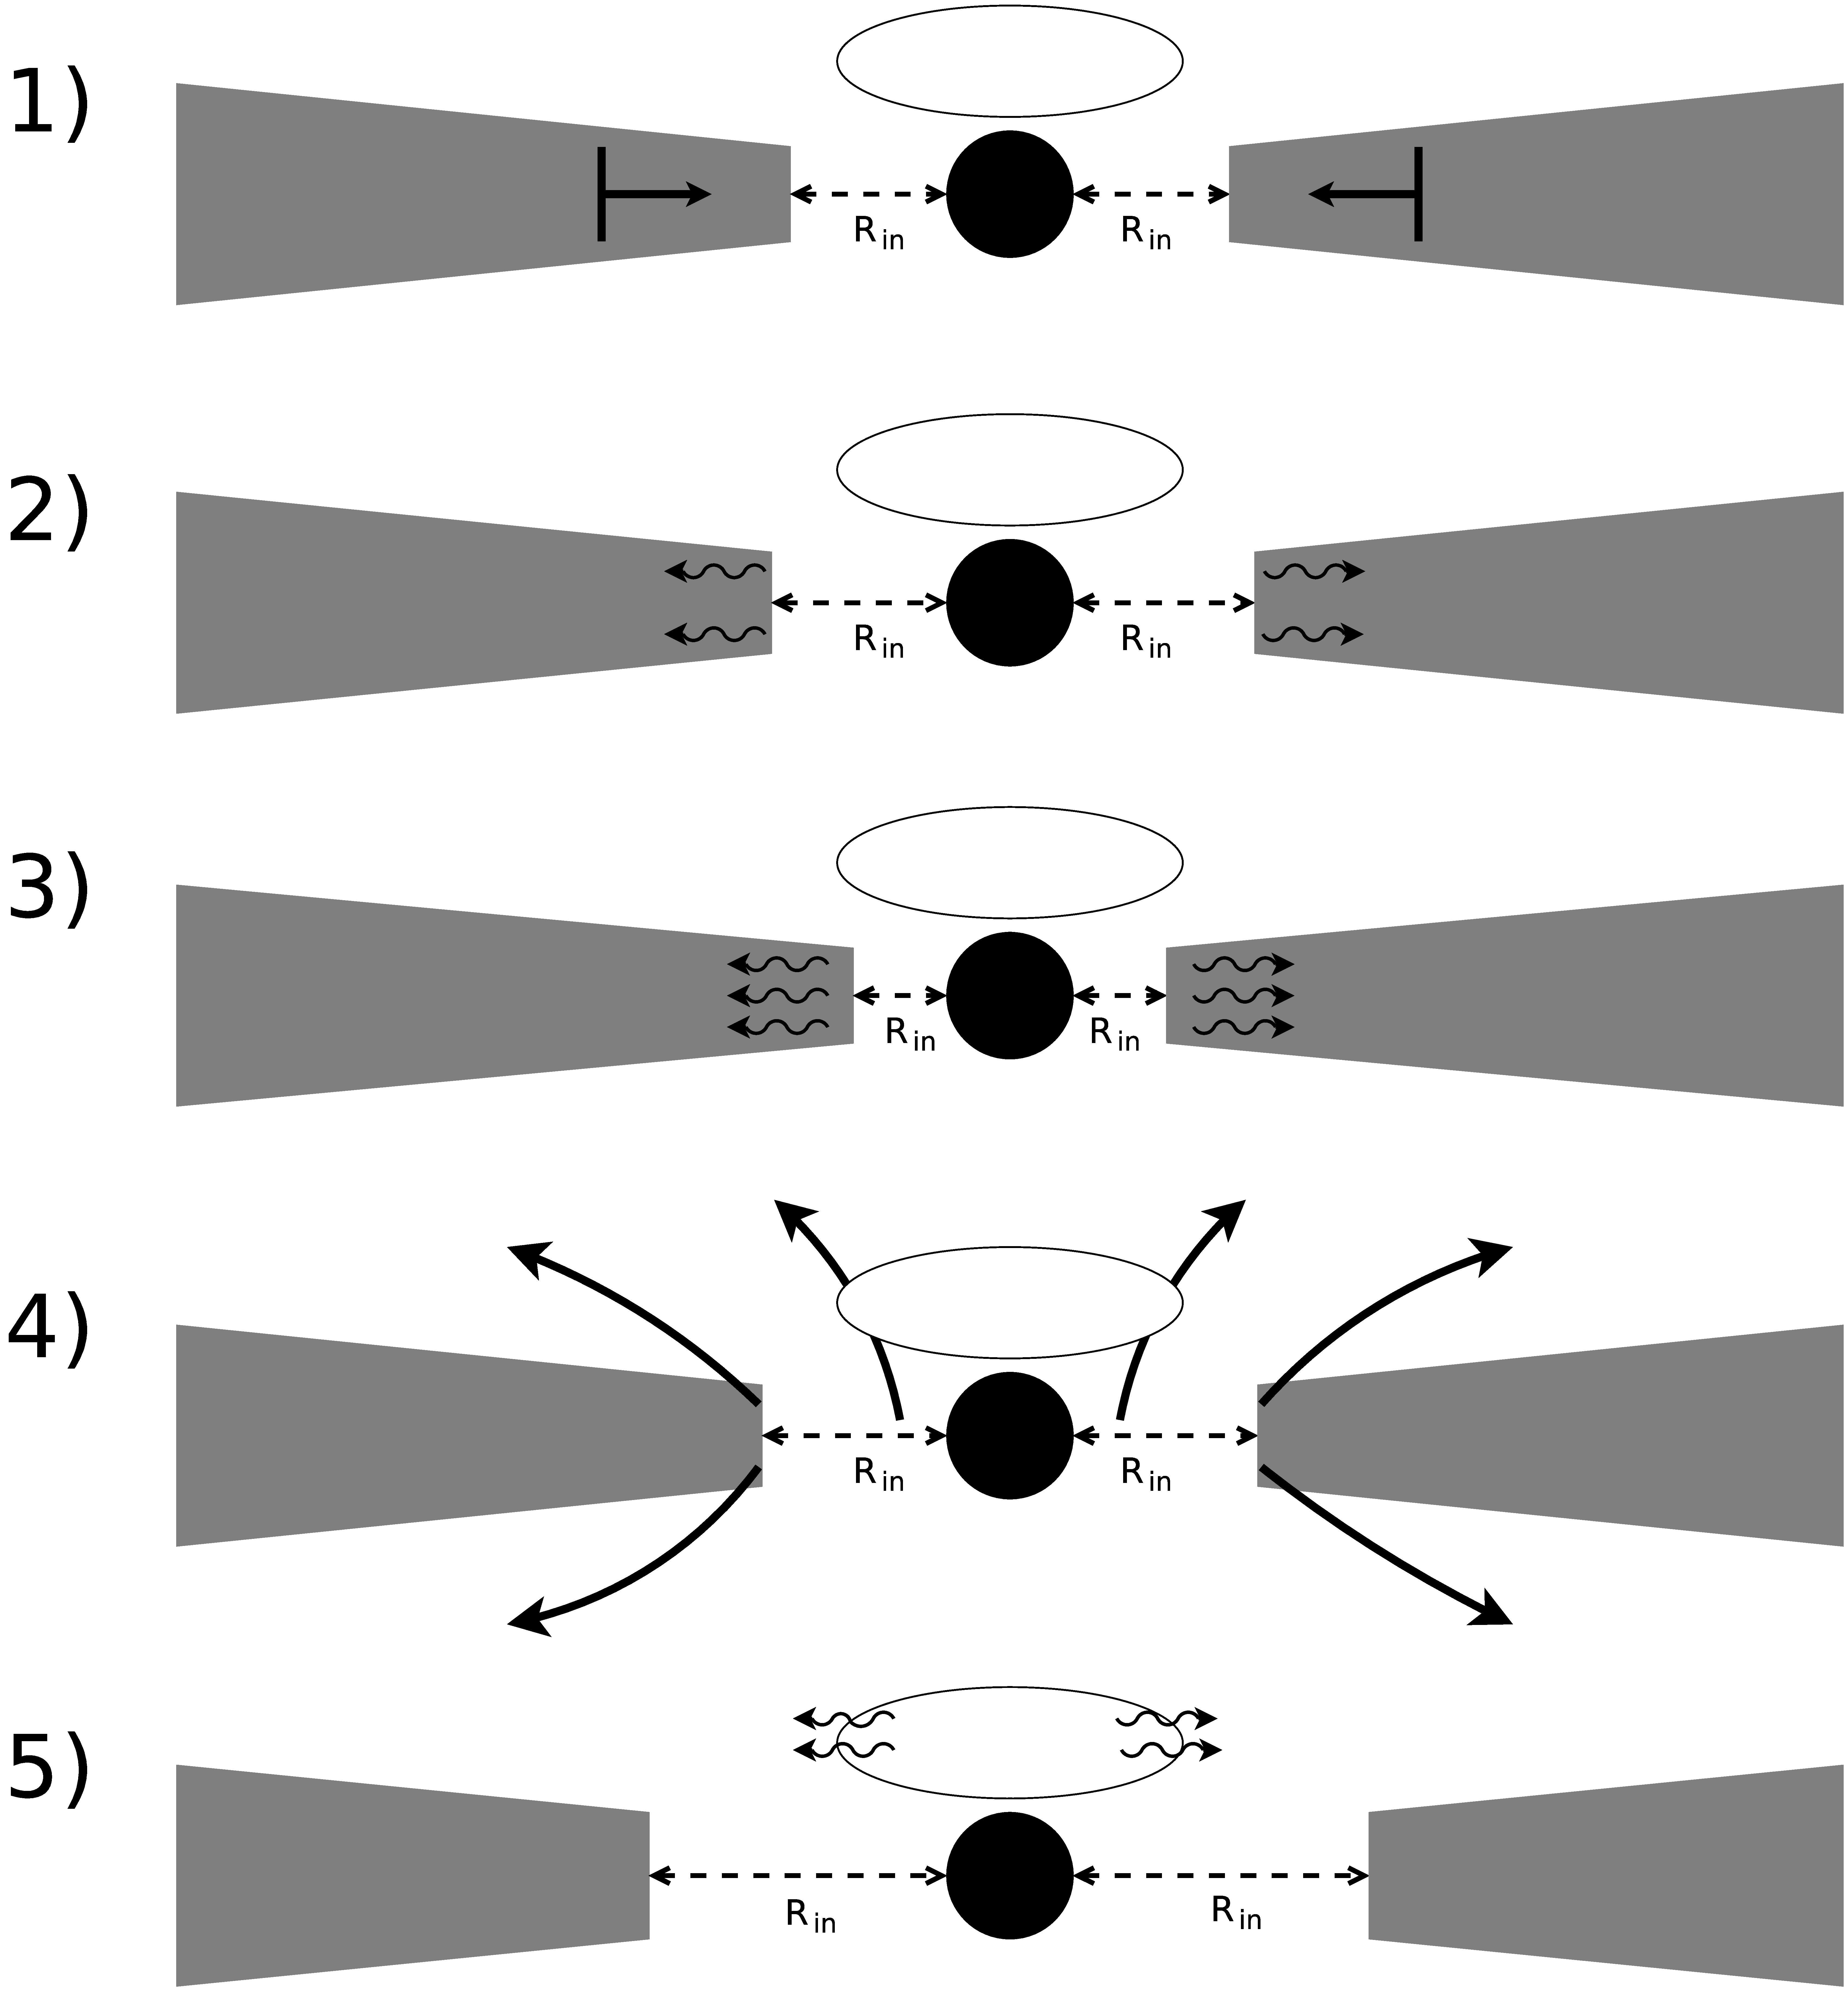
\includegraphics[width=.9\linewidth, trim= 25mm 0mm 0mm 0mm]{images/Wind_Model1.eps}
  \caption{\small A schematic diagram illustrating the the process described by \citet{Neilsen_GRSModel} to describe the $\rho$ variability class in GRS 1915+105.  1) The X-ray emission from the system originates from both the accretion disc truncated at an inner radius $r_{in}$ (grey) and a cloud of non-thermal electrons (white ellipse).  At some time $t$, an overdensity in the accretion disc (formed by the Lightman-Eardley Instability) propagates inwards towards $r_{in}$.  2) As the inner disc heats up, $r_{in}$ begins to slowly increase due to an increase in photon pressure.  This destabilises the disc.  3) At some critical density, the disc becomes too unstable and collapses inwards, greatly decreasing $r_{in}$ and raising the inner disc temperature.  4) The sudden increase in emission exceeds the local Eddington limit at $r_{in}$, ejecting matter from the inner accretion disc in the form of extreme winds.  5) Having been excited by matter in the winds passing through it, the non-thermal electron cloud emits a hard Brehmsstrahlung `pulse'.}
  \label{fig:WindsModel}
\end{figure}
\pagebreak

\par In their fitting, \citealp{Neilsen_GRSModel} consider three spectral models:
\begin{enumerate}
\item An absorbed disk black body with a high energy cutoff, of which some fraction has been Compton upscattered
\item An absorbed disk black body with a high energy cutoff, plus a Compton component with a seed photon spectrum tied to the emission from the disk
\item An absorbed disk black body plus a Compton component with a seed photon spectrum tied to the emission from the disk and a bremsstrahlung component
\end{enumerate}
They find that the first of these models (Model 1) is the best fit to the data.
\par \citealp{Mineo_PhasRes} also performed psuedo-phase-resolved spectroscopy of the $\rho$ class in GRS 1915, using a number of different spectral models to \citealp{Neilsen_GRSModel} but a significantly lower phase resolution.  In this work, the authors consider six models:
\begin{enumerate}
\item A multi-temperature disk black body plus a corona containing both thermal and non-thermal electrons (as forumlated by \citealp{Poutanen_Hybrid})
\item A multi-temperature disk black body plus a multi-temperature disk black body plus a power law
\item A multi-temperature disk black body plus an independent Compton component
\item A multi-temperature disk black body plus a power law plus reflection from the outer disk
\item A model of Comptonization due to the bulk-motion of matter in the disk
\item A multi-temperature disk black body plus a power law plus a standard black body
\end{enumerate}
With the exception of Models \textit{i} and \textit{vi}, the authors find that none of these models are able to satisfactorily fit the data in each of their phase bins independently.  As there is no reasonable physical explanation behind Model \textit{vi}, the authors only consider Model \textit{i}.  Their results suggest a large reduction of the corona luminosity during each heartbeat flare, which they interpret as the corona condensing onto the disk.  They also find that their results are consistent with GRS 1915 having a slim disk, but inconsistent with the hard lag being caused by photon upscattering in the corona.
\par \citealp{Massa_MoveLag} found that the magnitude of the lag between hard and soft photons in the $\rho$-class of GRS 1915 is not constant.  They found that the lag varies between $\sim3$--$10$\,s, and correlates strongly with count rate.  The magnitude of the lag, therefore, is too large to be simply due to a light travel time to the corona from the disk.  The authors suggest that their results are instead consistent the thermal adjustment of the inner disk itself as part of the instability limit cycle invoked to explain the flares.
\par \citealp{Massaro_Numerical} constructed a set of differential equations to mathematically explain the behaviour of the oscillator underlying $\rho$-like flaring in GRS 1915.  They find that a change between variability classes likely corresponds to a a change in global accretion rate, but that the accretion rate within the $\rho$ class is constant.  This model reproduces the count rate-lag correlation reported by \citealp{Massa_MoveLag}, as well as a previously reported correlation between flare recurrence time and count rate \citep{Massaro_Lag}.
\par \citealp{Mir_LagModel} instead propose a model of variability in the outer disk propagating inwards to the hotter inner disk.  They propose a model that explains both the hard lag of the fundamental frequency associated with the heartbeat flares, but also the hard lag of the first harmonic.  In contrast to the findings of \citealp{Massaro_Numerical}, their scenario requires a sinusoidal variation in the global accretion rate as a function of time.
\par More recently, \citealp{Zoghbi_Bulge} found that the reflection spectrum from GRS 1915 does not match what would be expected from the inner disk behaviour assumed by e.g. \citealp{Nayakshin_GRSModel}.  They again perform phase-resolved spectroscopy and fit a number of complex spectral models, finding that their data is best-described by the emergence of a bulge in the inner disk which propagates outwards during each flare.

\section{Type II Burst Sources}

xxxxx

\subsection{A History of Models of Type II Bursts}

\cleardoublepage

\chapter{Tools \& Methods}

\epigraph{\textit{The infinite is obvious and everywhere. To engage the finite takes courage.}}{Hunter Hunt-Hendrix -- \textit{Transcendental Black Metal}}

\vspace{1cm}

\par\noindent In this Chapter, I describe the tools and methods I employed as part of my studies.  In Section \ref{sec:sat} I describe the scientific instruments which were used to take the data I present in this thesis.  In Section \ref{sec:tec} I describe a number of methods and algorithms created by others which I make use of in my analysis.  I also present algorithms I have created as part of my studies.

\section{Instrumentation}

\label{sec:sat}

\par The atmosphere of the Earth is opaque to X-rays and gamma-rays, so we must use space-based observatories in order to study high-energy astrophysical phenomena.  A number of satellites dedicated to the study of X-rays have been launched over the years, starting with \textit{UHURU} in 1970 \citep{Giacconi_Uhuru} and culminating, most recently, with \textit{NICER} \citep{Gendreau_Nicer} and \textit{Insight} \citep{Li_HXMT} in 2017.  I use data from a number of these missions in the research reported in this thesis; in particular I use data from the NASA satellites \textit{RXTE}, \textit{Swift}, \textit{Chandra} and \textit{NuSTAR}, the European satellites \textit{XMM-Newton} and \textit{INTEGRAL}, and the Japanese satellite \textit{Suzaku}.  This section introduces the instruments used in my studies, as well as the tools used to extract their data for further analysis.

\subsection{The \textit{Rossi X-Ray Timing Experiment}}

\par The \textit{Rossi X-Ray Timing Experiment}, more commonly known as \textit{RXTE}, was a NASA-operated satellite launched from Cape Canaveral on December 30, 1995 \citep{Bradt_RXTE}.  \textit{RXTE} was primarily an X-ray observatory, constructed specifically to study X-ray variability seen in X-ray Binaries \citep{Bradt_XTEaims}.  The observatory operated until January 5, 2012, when it was decommissioned.
\par \textit{RXTE} carried three scientific instruments.  The main instruments were a pair of X-ray telescopes: the Proportional Counter Array (PCA, \citealp{Jahoda_PCA}) and the High Energy X-Ray Timing Experiment (HEXTE \citealp{Gruber_HEXTE}).  The satellite also carried an X-ray All-Sky Monitor (ASM, \citealp{Levine_ASM}).  PCA consisted of 5 Proportional Counting Units (PCUs) which were sensitive between $\sim2$--$60$\,keV.  The instrument had an excellent time resolution approaching 1\,$\mu$s, and an energy resolution of $\sim18\%$ at 6\,keV.  X-rays were guided onto the detectors by a collimator, resulting in an instrumental field of view with a full-width half-maximum of 1$^\circ$.  PCA had a 6500\,cm$^2$ collecting area, and no angular resolution.
\par The HEXTE instrument \citep{Gruber_HEXTE} provided complimentary coverage at higher energies, being sensitive in the $\sim15$--$250$\,keV range.  This instrument consisted 8 detectors, with a total collecting area of 1600\,cm$^2$, and had a similar field of view to that of PCA.  The time resolution was 8\,$\mu$s, and the energy resolution was 15\% at 60\,keV.
\par Finally, ASM was a soft X-ray all sky-monitor which covered 80\% of the sky every 90 minutes.  It was sensitive in the range 2--10\,keV, with a total collecting area of 90\,cm$^2$ and a spatial resolution of $3'\times15'$.  Due to its near continual coverage of the sky, ASM was excellent for long-term monitoring of transients in the soft X-ray sky.

\subsubsection{Data Formatting}

\par Much of the work in this thesis is based largely on data from PCA, which is freely available through the HEASARC archive maintained by NASA's Goddard Space Flight Centre\footnote{\url{https://heasarc.gsfc.nasa.gov/cgi-bin/W3Browse/w3browse.pl}}.  In PCA, as well as in other X-ray instruments, this data takes one of two forms:
\begin{itemize}
\item \textbf{Event-Mode Data:} A list of photon arrival times.  Depending on the instrument and observing mode, each of these times will have an associated channel, information about where in the detector the photon hit and a flag indicating the pattern that the photon made on the detector.
\item \textbf{Binned Data:} A list of evenly spaced time bins with the number of photons which arrived during each.  Depending on the instrument and observing mode, this may be accompanied by some information on the channel distribution of photons arriving in each bin.
\end{itemize}
\par The channel a photon falls into is determined by its energy, although the channel-to-energy conversion for a particular instrument changes over time as the instrument degrades or settings are altered.  The channel-to-energy conversions for PCA can be found at \url{https://heasarc.gsfc.nasa.gov/docs/xte/e-c_table.html}.
\par Both event-mode and binned-mode data are stored in a Flexible Image Transit System (\texttt{.fits}) format.  This is a hierarchical data format consisting of a number of `Header Data Units' (HDUs), each of which contains data in some format and a header with details of the format.  In addition to either an event list or a table of binned data, astronomical FITS files also contain a list of Good Time Intervals (GTIs) during which the satellite was functioning normally, as well as an amount of housekeeping information such as the start and end times of the observation.
\par For PCA observations of faint objects, event mode data with full energy information (referred to as \texttt{goodxenon}-mode data) is generally available.  However when brighter objects were observed, telemetry constraints sometimes prevented this full information from being transmitted to Earth.  In all observations, a number of alternative data products are available; \texttt{Standard1} data (binned data with 0.125\,s time resolution but no energy information), \texttt{Standard2} data (binned data with 16\,s time resolution, divided into 128 bins by channel) and a number of other data products with various time and energy resolutions.  While \texttt{Standard2} data are useful for studying spectral variability over long timescales, they is not useful for studying the second-to-minute scale variability reported on in this thesis.  I use \texttt{goodxenon} data when available, as this allowed us to use the maximum possible time and energy resolutions, and various other datamodes including \texttt{Standard1} when \texttt{goodxenon} mode data were not available.

\subsubsection{Data Extraction \& Background Correction}

\par To perform science with PCA or other instruments, one must extract science products (such as lightcurves, power spectra and energy spectra) from the raw data.  Tools to create lightcurves and power spectra from PCA data are available as part of \texttt{FTOOLS} \footnote{\url{https://heasarc.gsfc.nasa.gov/ftools/}}, a free NASA-maintained suite of software for manipulating \texttt{.fits} formatted data.  These scripts make use of CALDBs: freely available databases of calibration files provided by NASA for a number of active and historical X-ray telescopes (e.g. \citealp{Graessle_ChaCALDB}).  I also wrote my own software \texttt{PANTHEON} (Python ANalytical Tools for High-energy Event-data manipulatiON, presented in Appendix \ref{app:PAN}) to extract a number of additional products, such as power spectra and spectrograms.
\par In astronomy, the general way to subtract background from data is by selecting an empty piece of sky from the same observation as the source of interest, and then subtract one from the other.  However as PCA had no imaging capability, this is not possible to do with PCA data.  Instead, the \textit{RXTE} Guest Observatory Facility provides background models, which estimate the background of an observation based on the known X-ray background near the pointing direction and how the radiation environment of the spacecraft changes over its orbit.  Two background models are available, for faint\footnote{\url{http://heasarc.gsfc.nasa.gov/FTP/xte/calib_data/pca_bkgd/Faint/pca_bkgd_cmfaintl7_eMv20051128.mdl}} ($<40$\,cts\,s$^{-1}$\,PCU$^{-1}$) and bright\footnote{\url{http://heasarc.gsfc.nasa.gov/FTP/xte/calib_data/pca_bkgd/Sky_VLE/pca_bkgd_cmbrightvle_eMv20051128.mdl}} ($>40$\,cts\,s$^{-1}$\,PCU$^{-1}$) sources; these can be used in conjunction with the \texttt{pcabackest} tool in \texttt{FTOOLS} to automatically subtract the estimated background from binned PCA data.
\par As the PCA background models do not subtract the contributions from other sources in the field of view, I also use a different technique to subtract background from observations of GRO J1744-28 (which is in a very crowded region of the sky near the Galactic centre).  To try and account for these other sources, I instead chose an observation of the region of GRO J1744-28 taken while this source was in quiescence; I assume that all photons in this observation must be from the particle background, the cosmic background or another source in the field of view.  Although this method does subtract some of the background contributed from other sources in the field, it must be treated with caution as these other sources are likely also variable.
\par To compare photometry data from PCA with data from other instruments, I normalise the data by the flux from the Crab nebula.  The Crab is a commonly used reference source in astronomy due to its apparent brightness and low variability across a wide portion of the electromagnetic spectrum.  To Crab-normalise PCA data from a given observation, I take the PCA observation of the Crab which is closest in time to the observation of interest and in the same gain epoch.  This follows the method employed in \citet{Altamirano_CrabNorm}.
\par Long-term lightcurves from ASM are available on the ASM Light Curves Overview web page (\url{http://xte.mit.edu/asmlc/ASM.html}) maintained by MIT.

\subsection{The \textit{Neil Gehrels Swift Observatory}}

\par The \textit{Neil Gehrels Swift Observatory}, formerly and more commonly known as \textit{Swift}, is a NASA-operated satellite launched from Cape Canaveral on November 20, 2004 \citep{Gehrels_Swift}.  \textit{Swift} was specifically designed to study Gamma Ray Bursts (GRBs), and is notable for its fast slew speed.
\par \textit{Swift} carries three instruments: the X-Ray Telescope (XRT, \citealp{Burrows_XRT}), the wide field-of-view hard X-ray Burst Alert Telescope (BAT, \citealp{Krimm_BAT}) and an UltraViolet/Optical Telescope (UVOT, \citealp{Roming_UVOT}).  XRT is the primary instrument on \textit{Swift}: it is a focusing telescope with an effective energy range of 0.2--10\,keV.  Unlike PCA, XRT has imaging capabilities, with a field of view with a radius of 23.6' and an angular resolution of 18''.  The telescope has a minimum time resolution of 1.8\,ms and a minimum energy resolution of $\sim5$\% at 6\,keV.  XRT is operated in one of a number of `operating modes' during each observation, depending on the requirements of the observer.  The two main observing modes are:
\begin{enumerate}
\item Proportional Counting (PC) Mode: a full 2-dimensional image every 2.5\,s.
\item Windowed Timing (WT) Mode: a 1-dimensional image every 2.8\,ms.
\end{enumerate}
Both PC and WT modes also contain full energy information.
\par The main purpose of the wide area BAT telescope is to identify gamma ray bursts as soon as possible after they begin, so that \textit{Swift} can then slew to them for follow-up observation with XRT.  Due to its large field of view (1.4\,sr) and effective energy range of 15--150\,keV, BAT also provides us with long-term hard X-ray lightcurves of many bright sources in the X-ray sky.  It has a detecting area of 5200\,cm$^2$ and, when operating in survey mode, a time resolution of 5 minutes.
\par The final instrument, UVOT, is intended to take simultaneous optical and ultraviolet observations of sources observed with XRT.  It observes in the wavelength range between 170-650\,nm, and has 7 filters.

\subsubsection{Data Extraction}

\par XRT and ASM data on non-GRB transients are available via online portals maintained by the University of Leicester\footnote{\url{http://www.swift.ac.uk/user_objects/}} and the Goddard Space Flight Centre\footnote{\url{https://swift.gsfc.nasa.gov/results/transients/}} respectively.  The University of Leicester portal automatically extracts lightcurves, spectra, images and source positions from raw XRT data of a given target, using the \texttt{xrtpipeline} provided in \texttt{FTOOLS}.  The Goddard Space Flight Centre provides ready-made 15--50\,keV lightcurves of 1019\footnote{Count as of May 2018.} X-ray transients, with cadences of either 1 per day or 1 per \textit{Swift} orbit.

\subsection{The \textit{X-Ray Multi-Mirror Mission}}

\par The \textit{X-Ray-Multi Mirror Mission} (\textit{XMM-Newton}, \citealp{Jansen_XMM}) is an ESA-operated satellite which was launched from Kourou, French Guiana on December 10, 1999, and is still operating almost 20 years later.  Like \textit{RXTE} and \textit{Swift}, \textit{XMM-Newton} also carries a number of separate instruments: namely the European Photon Imaging Camera (EPIC, \citealp{Bignami_EPIC}), the Reflection Grating Spectrometer (RGS, \citealp{denHerder_RGS}) and an Optical Monitor (OM, \citealp{Mason_OM}).  In the research presented in this thesis, I only make use of data from EPIC.
\par EPIC consists of three CCD cameras which work independently: two metal-oxide semiconductor CCD cameras (EPIC-MOS1 and EPIC-MOS2) and a single pn CCD camera at the focus of the telescope (EPIC-pn).  All cameras observe in the energy range 0.15--15\,keV, with a Field of View of 30', an angular resolution of 6'' and a maximum energy resolution of $\sim5$\%.  The detectors can be operated in full frame, partial window or timing mode, each of which has a greater time resolution but narrower field of view than the last.  The maximum time resolution achievable by EPIC is 7\,$\mu$s which EPIC-pn is operated in burst mode; a special pn-only variant of timing mode.

\subsubsection{Data Extraction \& Processing}

\par \textit{XMM-Newton} data are extracted and processed using the \texttt{SAS} software \citep{Ibarra_sas} provided by ESA\footnote{\url{https://www.cosmos.esa.int/web/xmm-newton/sas}}.  These make use of the continuously updated Current Calibration Files (CCF), also provided by ESA.
\par The process of extracting basic data products from the EPIC instruments can be reduced to a number of steps:
\begin{itemize}
\item Use the \texttt{SAS} command \texttt{cifbuild} to create a Calibration Index File (CIF), containing pointers to the information in the CCF needed to reduce the chosen dataset.
\item Use the \texttt{SAS} command \texttt{odfingest} to create a summary file, containing data corrected by the CCF and by the EPIC housekeeping files.
\item Construct a photon event list from EPIC-MOS1 and EPIC-MOS2 using the \texttt{SAS} command \texttt{emproc}, or from EPIC-pn using the command \texttt{epproc}.
\end{itemize}
The event lists that result from this process can then be filtered using \texttt{evselect}, which allows the user to sort photons by arrival time, spatial co-ordinate and energy channel, among other parameters.  These filtered event lists can then be used to create science data products, such as lightcurves and energy spectra.

\subsection{\textit{Chandra}}

\par The \textit{Chandra X-Ray Observatory} (\textit{Chandra}, \citealp{Weisskopf_Chandra}) is a NASA-operated satellite which was launched from Cape Canaveral on July 23, 1999 aboard Space Shuttle \textit{Columbia}.  The mission is considered to be one of NASA's `Great Observatories', along with the \textit{Hubble Space Telescope} (\textit{HST}, e.g. \citealp{Holtzman_Hubble}), the \textit{Compton Gamma Ray Observatory} (\textit{CGRO}, \citealp{Gehrels_CGRO}) and the \textit{Spitzer Space Telescope} (\textit{Spitzer}, \citealp{Fanson_Spitzer}), which collectively observed the sky between infrared and gamma-ray wavelengths.  \textit{Chandra} was designed to study the X-ray sky between $\sim$0.1--10\,keV, and contains two instruments: the High Resolution Camera (HRC, \citealp{Kenter_HRCI}) and the Advanced CCD Imaging Spectrometer (ACIS, \citealp{Nousek_ACIS}).  The spacecraft also carries High and Low Energy Transmission Gratings (HETGS and LETGS respectively, \citealp{Markert_HETG,Brinkman_LETG}), which can be used in conjunction with the aforementioned detectors to produce high-resolution energy spectra.
\par HRC contains two detectors: the HRC Imager (HRC-I) and the HRC Spectrogram (HRC-S).  HRC-I has the largest field of view of any instrument aboard Chandra (30$\times$30'), but no time resolution and only poor spectral resolution.  HRC-S is a long-thin detector strip which is intended to be used as the readout for the LETG.  This detector can also be used in Fast Timing mode, in which it has no energy resolution but a timing resolution of 16\,$\mu$s.
\par ACIS is intended for use either as an imaging camera or as a detector for the output of the HETG.  It has a primary field of view of $16.9\times16.9$', and operates at a maximum time resolution of 2.85\,ms.

\subsubsection{Data Extraction \& Processing}
\par Like \textit{XMM-Newton}, \textit{Chandra} data are analysed using a purpose-built suite of tools.  The software for \textit{Chandra} analysis is named \texttt{Ciao} \citep{Fruscione_Ciao}, and is freely provided by Harvard University\footnote{\url{http://cxc.harvard.edu/ciao/}}.  \texttt{Ciao} filters and bins data based on any of the four possible parameters stored for a photon event (time, energy and two spatial co-ordinates), and facilitates the production of lightcurves, images and energy spectra.

\subsection{\textit{Suzaku}}

\par \textit{Suzaku} \citep{Mitsuda_Suzaku} was a JAXA-operated satellite which operated from its launch from the Uchinoura Space Center on July 10, 2005 until being decomissioned on September 2, 2015.  The mission was intended for X-ray spectroscopy; however the satellite's primary instrument, the X-Ray Spectrometer (XRS, \citealp{Kelley_XRS}), lost all of its liquid helium coolant within the first month of operation, rendering it effectively unusable.  The remaining instruments aboard \textit{Suzaku}, namely the X-Ray Imaging Spectrometers (XIS, \citealp{Koyama_XIS}) and the Hard X-Ray Detector (HXD, \citealp{Takahashi_HXD}) were unaffected by the malfunction and continued to operate normally throughout the spacecraft's lifetime.
\par XIS consists of four X-ray cameras, with a total field of view of $18\times18$'' and a spatial resolution of $\geq1.6$''.  The instrument has a good spectral resolution over its operational energy range of 0.2--10\,keV, peaking at $\sim170$\,eV at the upper end of this range.  Standard observation XIS observation modes provide no timing information, and as such the time resolution is limited to the 8\,s duration of a single CCD exposure; this timing resolution can be improved by a factor of a few by sacrificing imaging information in the instrument's clocking mode.
\par HXD complements XIS at higher energies, with an effective energy range of 10--600\,keV.  The instrument has an energy resolution of $\sim3$\,keV below 60\,keV, and $\sim7$--8\% above 60\,keV.  The instrument has an optimum time resolution of 7.8\,ms.
\par As with most instruments, there exist standard procedures when reducing and analysing data from \textit{Suzaku}.  First of all, the data must be reprocessed using the \texttt{aepipeline} script available as a part of HEASOFT.  Lightcurves, images and spectra can then be extracted using the standard multimission tools available in FTOOLS.  Note that, for XIS, backgrounds for each of the four detectors should be extracted separately due to differential degradation over the lifetime of the mission.

\subsection{\textit{NuSTAR}}

\par The \textit{Nuclear Spectroscopic Telescope Array} (\textit{NuSTAR}, \citealp{Harrison_NuStar}) is a NASA-operated satellite launched from the \textit{Stargazer} aircraft off the coast of the Marshall Islands on June 13, 2012.  The satellite carries two co-pointing X-ray telescopes, which are matched with Focal Plane Modules referred to as FPMA and FPMB.  These detectors are sensetive and calibrated in the range 3--78\,keV, and each has an effective are which maximises at $\sim450$\,cm$^2$ at $\sim10$\,keV.  The telescopes have a field of view of $12.2\times12.2$', and a full-width half-maximum angular resolution of $\gtrsim18$''.  Events are detected by \textit{NuSTAR} with an arrival time error of $\sim\pm3$\,ms, while the energy resolution at 50\,keV is around 0.4\,keV.
\par For the research presented in this thesis, I reduce data from \textit{NuSTAR} using the \texttt{nupipeline} script from the freely available \textit{NuSTAR} Data Analysis Software (NuSTARDAS\footnote{\url{https://heasarc.gsfc.nasa.gov/docs/nustar/analysis/nustar_swguide.pdf}}).  This script automatically runs all of the relevant tasks required to reduce \textit{NuSTAR} data, including flagging of events, flagging of bad pixels and correcting for detector gain.  It also calculates sky co-ordinates and energy for each event.

\subsection{\textit{INTEGRAL}}

\par The \textit{INTernational Gamma-Ray Astrophysics Laboratory} (\textit{INTEGRAL}, \citealp{Winkler_INTEGRAL}) is an ESA-operated satellite which was launched from Kazakhstan's Baikonur Cosmodrome on October 17, 2002.  The primary purpose of the mission is the spectroscopy of astrophysical sources in the hard X-ray and soft gamma-ray bands, between $\sim4$--10,000\,keV.
\par \textit{INTEGRAL} carries two main scientific instruments: the SPectrometer on \textit{INTEGRAL} (SPI, \citealp{Vedrenne_SPI}) and the Imager on-Board \textit{INTEGRAL} (IBIS, \citealp{Winkler_IBIS}).  The spacecraft also carries an X-ray monitor (JEM-X, \citealp{Schnopper_JEMX}) and an optical camera (OMC, \citealp{Gimenez_OMC}).
\par SPI is a high-resolution gamma-ray spectrometer, with an energy resolution of $\sim$2.2\,keV at 1.33\,MeV and an energy range of 18\,keV to 8\,MeV.  It has a field of view of $>14^\circ$, an angular resolution of 2.5$^\circ$, a time resolution of 0.129\,ms and a collecting area of $\sim500$\,cm$^2$.
\par IBIS has a wider energy range than SPI, from 15\,keV to 10\,MeV, and a larger collecting area at 3100\,cm$^2$.  The timing accuracy is 61\,$\mu$s, but the energy resolution peaks at only 8\% at $\sim100$\,keV.  As IBIS is an imager, it has a good angular resolution of $\sim12$' and a field of view of $>8\times8$''.  IBIS contains two detector plains stacked on top of each other; the top layer (ISGRI, \citealp{Lebrun_ISGRI}) is designed to detect low-energy gamma rays, while the lower layer (PICsIT, \citealp{Labanti_Picsit}) is designed to detect the higher-energy gamma rays which pass through ISGRI undetected.
\par Data products from all four instruments are available via the \textit{INTEGRAL} Heavens portal \citep{Lubinski_Heavens} maintained by the \textit{INTEGRAL} Science Data Centre \footnote{\url{https://www.isdc.unige.ch/heavens/}}.  This portal provides images, lightcurves and spectra of data taken from archived \textit{INTEGRAL} observations.

\section{Methods \& Techniques}

\label{sec:tec}

\par To extract meaningful physics from the data provided by the space-based observatories described above, I use a number of mathematical and analytical techniques.  I analyse three main properties of the data:
\begin{enumerate}
\item \textbf{Lightcurve Morphology:} Measuring the luminosity of an object, particularly in relation to its Eddington luminosity, and describing how this luminosity changes over time.
\item \textbf{Timing Analysis:} Using Fourier and Lomb-Scargle spectroscopy to identify periodic and quasi-periodic features in the data, and how these change with energy and time.
\item \textbf{Energy Spectral Analysis:} Comparing the energy spectrum of the emission from this source, and how this changes over time, with models to predict the physical geometry and the mechanisms active in the system.
\end{enumerate}
\par Some of the techniques I used to explore these properties are detailed in this section.

\subsection{Lightcurve Morphology}

\label{sec:LCMorph}

\par The morphology of a lightcurve, how the brightness of a source varies over time, can tell us about the physical processes at work in the system.  For example, the rise and fall-times of an X-ray burst can be matched with characteristic physical timescales of an accreting system to better understand which of them play roles in generating the bursts.  However, quantifying these shapes over short timescales, or in datasets with large errors, can be difficult.  As such, methods exist to help analyse the morphology of these difficult datasets, and I employ a number of them in the research presented in this thesis.

\subsubsection{Lightcurve Folding}

\par In systems with periodic or quasi-periodic behaviour, it is important to understand the morphology of a single cycle of the behaviour.  If the system is bright enough that there are good statistics on timescales shorter than that of the oscillation, this is trivial; however it is often the case that the behaviour of a single oscillation in fast or faint systems is difficult to discern.  Instead, one can take the average of many cycles, greatly increasing the signal-to-noise ratio of the data.  The process of obtaining this average cycle is known as `folding' data.
\par To fold a periodic dataset with a known period $p$, the time $t$ associated with each datapoint must be converted into a phase $\phi$ (for $0\leq\phi<1$) such that datapoints at the same stage of different oscillations have the same $\phi$.  This can be done using the formula:
\begin{equation}
\phi(t)=\Phi(t)\mod1=(t-t_0)/p\mod1=(t-t_0)/p-N_t
\label{eq:simfold}
\end{equation}
Where $\Phi(t)$ is the fractional number of cycles which have elapsed between times $t_0$ and $t$ for an arbitrary start time $t_0$, and $N_t$ is the integer number of complete cycles which have occured between times $t_0$ and $t$.
\par This procedure can also be thought of as cutting a lightcurve into a number of pieces each of length $p$, and finding fractionally how far along each point is along the piece in which it falls.  Once this information has been found for all datapoints, the data can be rebinned in $\phi$-space to `stack` every cycle on top of one another.  I illustrate this process visually in Figure \ref{fig:Folding}.  This method is useful for finding mean oscillation profiles when $p$ is very close to a constant, such as finding the mean pulse profile of a pulsar over a small number of rotations.  However in many cases, such as in quasi-periodic oscillations (QPOs), $p$ is not a constant.  More complex methods must then be used to find the mean pulse profile.

\begin{figure}
    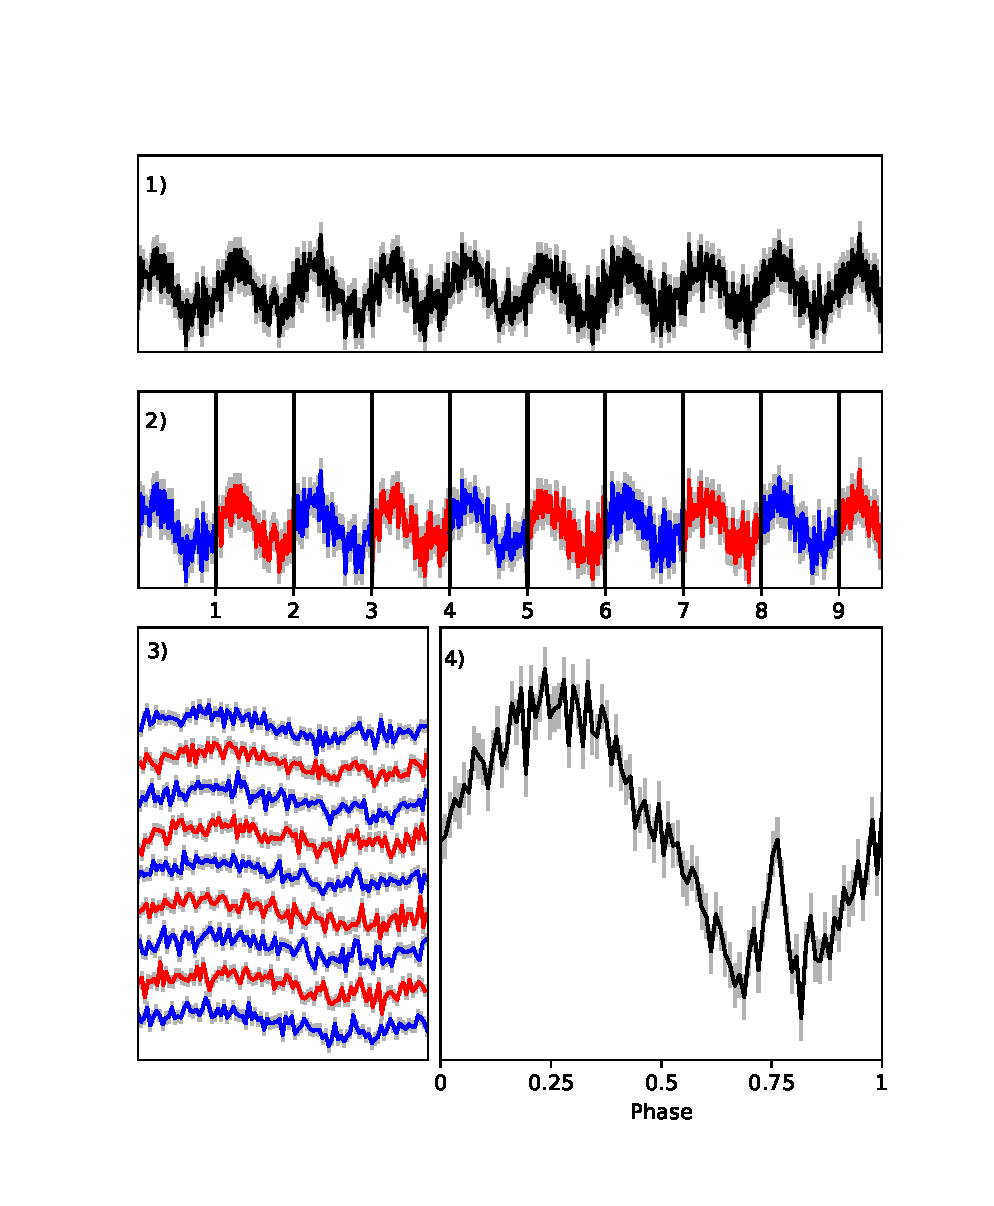
\includegraphics[width=\columnwidth, trim = 0mm 20mm 0mm 28mm]{images/folding.eps}
    \captionsetup{singlelinecheck=off}
    \caption[A cartoon illustrating the process of folding a periodic lightcurve with a known period.]{A cartoon illustrating the process of folding a periodic lightcurve with a known period.  \textbf{1:} a simulated lightcurve with errors.  \textbf{2:} Divide the lightcurve into sections by cutting it at every time coordinate $Np$, where $p$ is the known period and $N$ is any integer.  Each data point may now be given a phase coordinate $\phi$ in addition to its time coordinate $t$, where $\phi=(t/p)-N$ for $N$ such that $0\leq\phi<1$.  \textbf{3:} The lightcurve segments can be realigned in phase-space, such that points with the same value of $\phi$ sit at the same $x$-coordinate.  \textbf{4:} All points within given bins in $\phi$-space are averaged to create a lightcurve corresponding to the averaged oscillations of the original lightcurve.  The folding has revealed a peak at $\phi=0.75$ which was not apparent in the unfolded data.}
   \label{fig:Folding}
\end{figure}

\subsubsection{Flare-Finding Algorithm}
\label{sec:Flares}

\par To fold a quasi-periodic oscillation, such as the `heartbeat' flares seen in GRS 1915+105 and IGR J17091-3624, it is first important to find the $t$-values which characterise the beginning, end and peak of each flare.  To this end, I have created an algorithm to locate individual flares in a dataset containing non-periodic high-amplitude flares. The algorithm is performed as such (illustrated visually in Figure \ref{fig:BurstAlg}):

\begin{enumerate}
  \item Choose some threshold values $T_L$ and $T_H$.  Set the y-value of all datapoints with $y<T_L$ to zero.
  \item Retrieve the $t$-co-ordinate of the highest value remaining in the dataset.  Call this value $t_m$ and store it in a list.
  \item Set the value of point at $t_m$ to zero.
  \item Scan forwards from $t_m$.  If the selected point has a nonzero value, set it to zero and move to the next point.  If the selected point has a zero value, move to step 5.
  \item Scan backwards from $t_m$.  If the selected point has a nonzero value, set it to zero and move to the previous point.  If the selected point has a zero value, move to step 6.
  \item Retrieve the y-co-ordinate of the highest value remaining in the dataset.  Call this $y_m$.
  \item If $y_m>T_H$, repeat steps 2--7.  If $y_m<T_H$, proceed to step 8.
  \item Restore the original dataset.
  \item Retrieve the list of $t_m$ values found in step (ii).  Sort them in order of size.
  \item For each pair of adjacent $t_m$ values, find the $t$-coordinate of the datapoint between them with the lowest y-value.  Call these values $t_c$.
  \item This list of $t_c$ can now be used to demarcate the border between peaks.
\end{enumerate}

\begin{figure}
    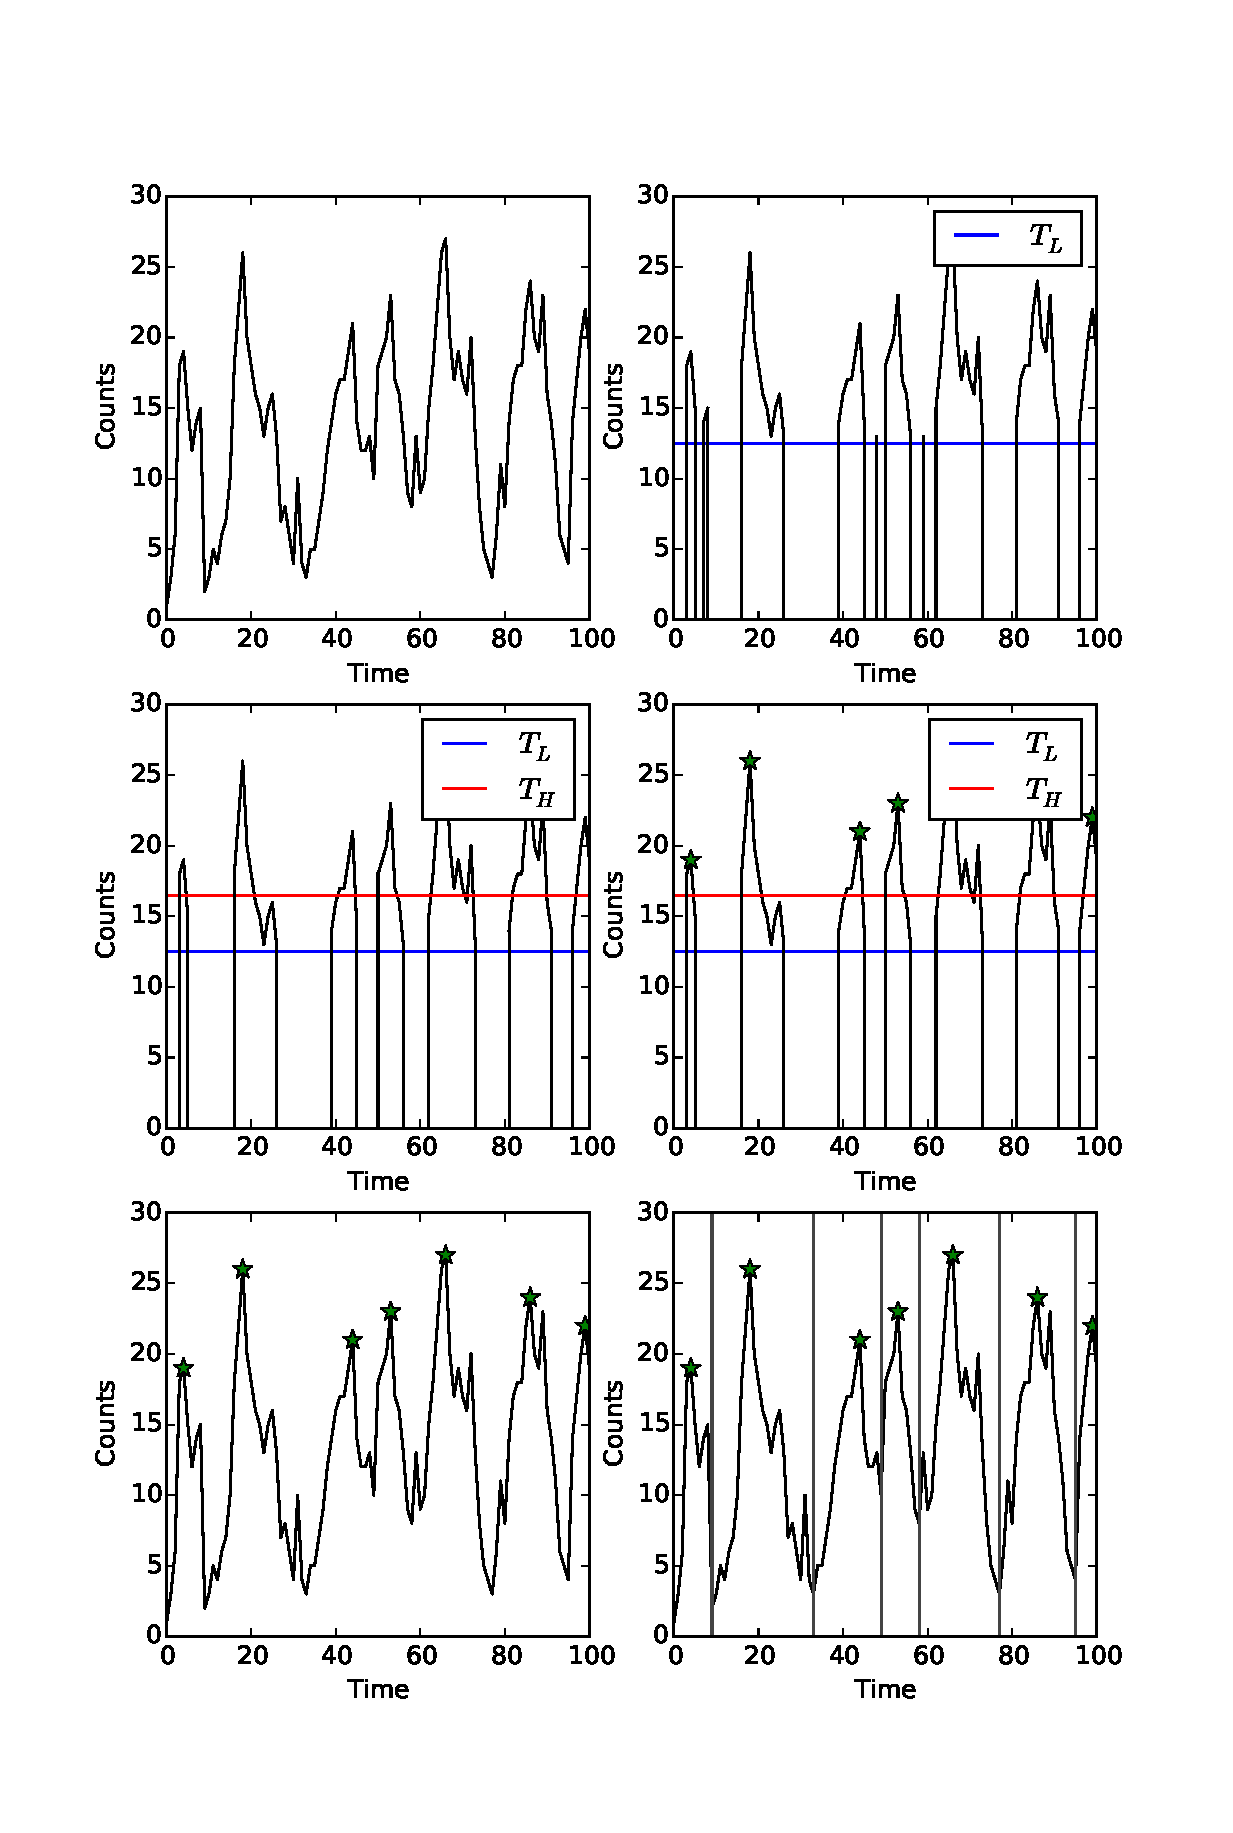
\includegraphics[width=\columnwidth, trim = 0mm 30mm 0mm 28mm]{images/steps.eps}
    \captionsetup{singlelinecheck=off}
    \caption[A cartoon illustrating the procedure of the algorithm described in Section \ref{sec:Flares}.]{From top-left: (i) An untouched data-set.  (ii) The dataset with all $y<T_L$ removed.  (iii) The dataset with all contiguous nonzero regions with $\max(y)<T_H$ removed.  (iv) The $t$-coordinates of peak $y$-values $t_m$.  (v) The restored dataset with the $t_m$ highlighted.  (vi) The boundaries between adjacent peaks.}
   \label{fig:BurstAlg}
\end{figure}

The values $T_L$ and $T_H$ can also be procedurally generated for a given piece of data:

\begin{enumerate}
  \item Select a small section of the dataset or a similar dataset (containing $\sim20$ peaks by eye) and note the time-coordinates $t_e$ of all peaks found by eye.
  \item Let $P_L$ and $P_H$ be two arbitrary values in the range $[0,100]$.
  \item Let $T_L$ ($T_H$) be the $P_L$th ($P_H$th) percentile of the y-values of the subsection of dataset.
  \item Run the flare-finding algorithm up to step 9.  Save the list of $t_m$.
  \item Split the dataset into bins on the x-axis such as the bin width $b\ll p$, where $p$ is the rough x-axis separation between peaks.
  \item For each bin, note if you found any value in $t_m$ falls in the bin and note if any value of $t_e$ falls in the bin.
  \item Using each bin as a trial, compute the Heidke Skill Score \citep{Heidke_SKSC} of the algorithm with the method of finding peaks by eye:
  \begin{equation}HSS = \frac{2(AD-BC)}{(A+B)(B+D)+(A+C)(C+D)}
  \label{eq:HSS}
  \end{equation}
  Where $A$ is the number of bins that contain both $t_e$ and $t_m$, $B$ ($C$) is the number of bins that contain only $t_m$ ($t_e$) and $D$ is the number of bins which contain neither \citep{Kok_YesNo}.
  \item Repeat steps (iii)--(vii) for all values of $P_H>P_L$ for $P_L$ and $P_H$ in $[1,100]$.  Use a sensible value for the resolution of $P_L$ and $P_H$.  Save the HSS for each pair of values
  \item Locate the maximum value of HSS, and note the $P_L$ and $P_H$ values used to generate it.  Use these values to generate final $T_L$ and $T_H$ values.
\end{enumerate}

I show an example of Heidke skill score grid for this algorithm, applied to a Class IV observation, in Figure \ref{fig:Heidke}.

\begin{figure}
    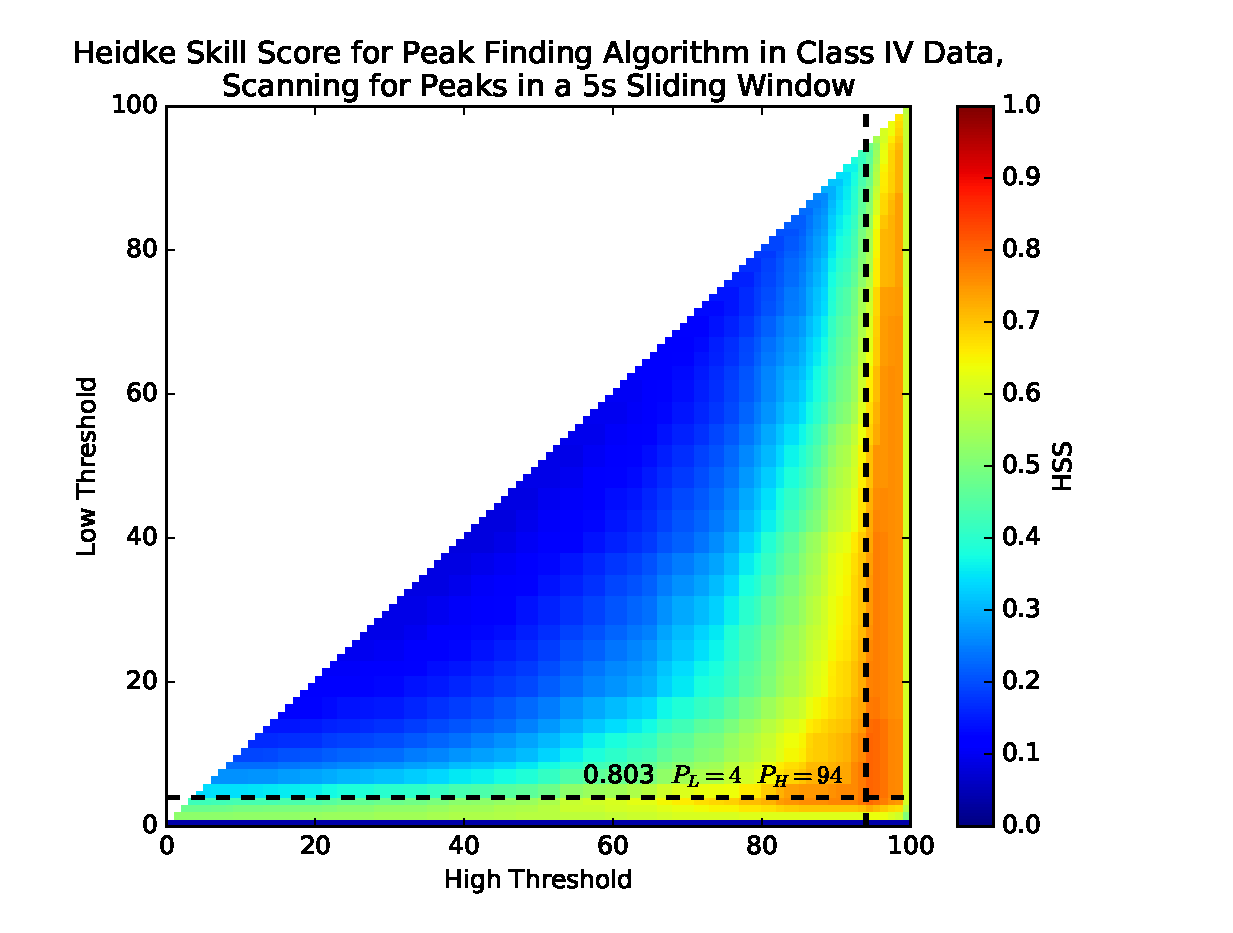
\includegraphics[width=\columnwidth, trim = 0mm 10mm 0mm 10mm]{images/HSS_J.eps}
    \captionsetup{singlelinecheck=off}
    \caption[The Heidke Skill score of a Class IV observation of IGR J17091-3624 for a selection of different values $P_L$ and $P_H$ (low and high threshold respectively).]{The Heidke Skill score of a Class IV observation of IGR J17091-3624 for a selection of different values $P_L$ and $P_H$ (low and high threshold respectively).}
   \label{fig:Heidke}
\end{figure}

\subsubsection{Variable Period Lightcurve Folding}

\par With the values $t_m$ and $t_c$ found using the algorithm described above, it is possible to recast Equation \ref{eq:simfold} to fold data over a high-amplitude but quasi-periodic oscillation.  I detail my method below:

\begin{enumerate}
  \item Take the ascending list of peak $t$-coordinates $t_m$.  Assign the first element a value $\Phi=0$.
  \item Assign each other point in $t_m$ an integer value $\Phi(t)$, such that the $\Phi$ value of the $i$th value of $t_m$ is defined as:
  \begin{equation}
  \Phi(t_m^{i})=\Phi(t_m^{i-1})+1, i\geq2
  \end{equation}
  \item If the troughs between bursts are well-defined, proceed to step 4.  Otherwise, skip to step 6.
  \item If the $t$-coordinate of the first datapoint in $t_c$ is less than the $t$-coordinate of the first datapoint in $t_m$, assign $\Phi(t_c^1)=-0.5$.  Otherwise, assign $\Phi(t_c^1)=-0.5$.
  \item Assign each other point in $t_m$ a value $\Phi(x)$, such that the $\Phi$ value of the $i$th value of $t_c$ is defined as:
  \begin{equation}
  \Phi(t_c^{i})=\Phi(t_c^{i-1})+1, i\geq2
  \end{equation}
  \item Create a general function defining $\Phi$ for all $t$ by fitting the $t$ and $\Phi$ values of $t_m$ (and $t_c$, if used) with a monotonically increasing univariate cubic spline\footnote{Computationaly realised as \texttt{PchipInterpolator} in the \texttt{scipy} package for Python \citep{NumPy}.} $S(t)$.
  \item Define the phase $\phi(t)$ of an arbitrary time $t$ as $\phi(t)=S(t)\mod1$.
\end{enumerate}

\par With a phase defined for all points in time, the data can be manipulated as if it had been folded in the usual way.  If the trough times in addition to the peak times are used to construct the spline, then the folded data are more accurate: however, by definition the rising part of each flare will occupy phases 0.5--1.0, while the falling part will occupy 0.0--0.5, so any assymetry in the rise and fall times of the average flare is lost.

\subsection{Timing Analysis}

\par Another way of looking at the variability of an astrophysical source is by looking in the frequency domain.  Well-established mathematical techniques, in particular Fourier spectroscopy, are able to deconvolve a time series into series of sine waves.  The amplitudes of these sine waves indicate how much variability in the system takes place at a given frequency.

\subsubsection{Fourier Spectroscopy}

\par Fourier Spectroscopy \citep{Fourier} is the most common way to perform frequency analysis on a time series.  The Fourier transform $\hat{f}(\nu)$ of a time series $f(t)$ is defined as:
\begin{equation}
\hat{f}(\nu)=\int_\infty^\infty f(t)e^{-2\pi it\nu} dt
\end{equation}
Where $\nu$ is the frequency to be probed and $i\equiv\sqrt{-1}$.  The magnitudes of the complex values $\hat{f}(\nu)$ describe the amplitude of the sine wave deconvolution at frequency $\nu$, while the arguments describe the relative phase of each of these sine waves.  As such, a plot of $|\hat{f}(\nu)|$ against $\nu$, known as a Fourier spectrum, highlights the frequencies at which the time series shows oscillations.  A strictly periodic oscillation shows up in a Fourier spectrum as a delta spike at a single frequency $\nu_p$; if the oscillation is not strictly sinusoidal, then there may also be spikes present at the harmonic frequencies $N\nu_p$ for any $N\in\mathbb{N}$.  A quasi-periodic oscillation shows up in a Fourier spectrum as a Lorentzian, defined by its amplitude and its quality factor $q$.  Quality factor is in turn defined as peak frequency divided by full-width half-maximum frequency width, and it represents approximately the number of oscillations over which the QPO remains coherent.
\par Fourier Spectroscopy was envisioned to analyse continuous, infinite data.  However, physical data differs from this ideal case in two important ways:
\begin{enumerate}
\item Physical data are discrete rather than continuous, consisting of samples taken at a finite rate $r$.
\item Physical data are finite rather than infinite, being taken in some window of length $w$.
\end{enumerate}
As such, as I show in Figure \ref{fig:convolve}, physical data consists of a time series convolved with both a windowing function and a sampling function.  Each of these convolutions adds spurious features to the power spectrum produced by the data.

\begin{figure}
    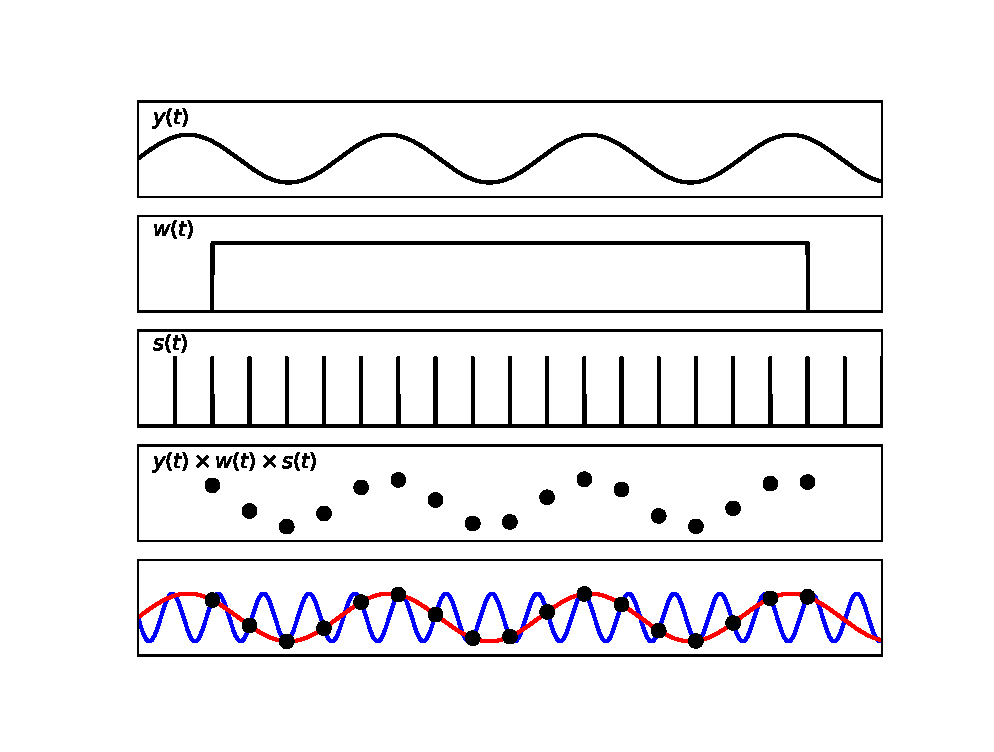
\includegraphics[width=\columnwidth, trim = 0mm 10mm 0mm 10mm]{images/convolve.eps}
    \captionsetup{singlelinecheck=off}
    \caption[A representation of how a continuous variable is convolved with a windowing function and a sampling function to yield physical data.]{A representation of how a continuous variable $y(t)$ is convolved with a windowing function $w(t)$ and a sampling function $s(t)$ to yield physical data.  The bottom panel shows how aliasing arises, showing that sine waves of two different frequencies can be fit to the data: one with a frequency $\nu$ equal to that in the original dataset, and one of frequency $\sigma-\nu$ where $\sigma$ is the sampling frequency.}
   \label{fig:convolve}
\end{figure}

\par The convolution with a sampling function adds so-called `aliased' peaks to the power spectrum of a given dataset.  For each peak in the power spectrum at frequency $\nu$, there will also be a peak present at a frequency of $\sigma-\nu$, where $\sigma$ is the sampling frequency.  This peak can be understood as the beat frequency between the oscillation in the data and the sampling frequency (see also the lower panel of Figure \ref{fig:convolve} for a visual explanation), and contains no additional information on the system.  To avoid these aliased peaks, values of $\hat{f}(\nu)$ outside of the range $0<\nu\leq\sigma/2$ are discarded.  The frequency $\sigma/2$, the maximum frequency at which one can extract useful information on a parameter sampled at constant frequency $\sigma$, is known as the Nyquist frequency.
\par The convolution with the windowing function causes peaks in the power spectrum to be broadened; an effect known as `spectral leakage'.  The form of this broadening depends on the windowing function which is being used.  Generally, physical data has been convolved with a so-called `boxcar' window; i.e., a function which takes a value of 1 during the period of measurement and 0 elsewhere.  A convolution with a boxcar window causes each peak in the power spectrum to be accompanied by a number of lower-amplitude sidelobes either side of it in frequency space; this serves to smear out a power spectrum and causes some information to be lost.  Other windows can be applied to data to attempt to lessen this effect; for example, convolving a dataset with a triangular or Gaussian windowinstead of a boxcar.  Many non-boxcar windows have been formulated to lessen the effect of spectral leakage, but it is impossible to remove the effect completely when working with a finite dataset.

\subsubsection{Fast Fourier Transform}

\par Taking the Fourier transform of a series is a computationally expensive procedure.  As such, it is common practice to instead use Fast Fourier Transform (FFT) algorithms; computationally fast algorithms which specialise in finding the Fourier transform of evenly-spaced series.
\par One such FFT algorithm is the Cooley-Tukey\footnote{Computationaly realised as \texttt{fft} in the \texttt{scipy.fftpack} package for Python \citep{NumPy}.} algorithm \citep{Cooley_FFT}.  The Cooley-Tukey algorithm speeds up the Fourier transform process by recursively dividing a datset in half to make many segments.  It uses the fact that the discrete Fourier transform of a single point is equal to itself, and then reconstructs the complete Fourier spectrum from these results. Unlike the basic Fourier transform, the Cooley-Tukey algorithm is only able to transform series which are evenly spaced in time and consisting of $2^N$ datapoints, for $N\in\mathbb{N}$.
\par The error on a Fast Fourier Transform of an arbitrary dataset is 100\%.  There are two ways to reduce this error to a level at which the data can be meaningfully analysed:
\begin{enumerate}
\item The original time series can be split into a number of equal-length windows.  The Fast Fourier-Transforms of these windows can be calculated independently of each other, and then averaged to create the mean FFT of the dataset.
\item The resultant power spectrum can be rebinned in frequency space.
\end{enumerate}
\par Propagating errors in the usual way, this results in a final error on Fourier power $\delta\hat{f}(\nu)$ of:
\begin{equation}
\delta\hat{f}(\nu)=\frac{\hat{f}(\nu)}{\sqrt{MW}}
\end{equation}
Where $W$ is the number of windows the original dataset was divided into, and $M$ is the number of frequency bins which were averaged to obtain the Fourier power at frequency $\nu$.  Increasing $W$ increases the minimum frequency at which the Fourier power of the dataset can be probed, while increasing $M$ removes information on the fine structure of the power spectrum.

\subsubsection{Normalising the Fourier Transform}

\par To understand the significance of features in a power spectrum, it is important to normalise the results in a standard and well-understood way.  One such method of normalisation is the `Leahy' normalisation \citep{Leahy_Norm}, defined as:
\begin{equation}
L(\nu)=\frac{2\times|\hat{f}(\nu)|^2}{n_{p}}
\end{equation}
Where $n_p$ is the total number of photon counts in the original dataset.  This normalisation has the property that pure Poisson noise has a Leahy-normalised power of 2\footnote{In practise, due to instrumental dead-time effects meaning photon arrivals are not strictly independent, Poisson noise in astrophysical data tends to yield a Leahy-normalised power of slightly less than 2}.
\par I use one additional power spectrum normalisation in the work presented in this thesis: the RMS normalisation.  This is defined as:
\begin{equation}
R(\nu)=\frac{(L(\nu)-2)r_s}{(r_s-r_b)^2}=\frac{2\left(|\hat{f}(\nu)|^2-Tr_s\right)}{T(r_s-r_b)^2}
\end{equation}
\par Where $T$ is the total time duration of all data used to produce the power spectrum, $r_s$ is the mean source count rate and $r_b$ is the mean background rate.  In this normalisation, Poisson noise corresponds to a power of zero.  Additionally, the power spectrum has the property that the integral of $R(\nu)$ between two frequencies is equal to the root-mean squared amplitude of the variability of the original time series in that frequency band.

\subsubsection{Lomb-Scargle Periodograms}

\par Fast Fourier transforms are unable to process unevenly spaced time series.  Additionally, while mathematical Fourier transforms can in general process unevenly spaced datasets, the effects of aliasing become increasingly complex and difficult to disentangle from real signal.  In these cases, a method known as the Lomb-Scargle periodogram, based on proposals by \citet{Lomb_LombScargle} and \citet{Scargle_LombScargle}, can be used.
\par The Lomb-Scargle periodogram can be thought of as the result of fitting sinusoids of frequency $\nu$ to a time series, and constructing a spectrum using the $\chi^2$ value of the fit of the sinusoid at each $\nu$.  Unlike a Fourier spectrum of unevenly spaced data, the Lomb-Scargle periodogram of unevenly spaced data is statistically well-behaved as long as the white-noise component of the dataset is uncorrelated.
\par Unfortunately, due to dead-time effects present in all X-ray telescopes, white noise in real datasets is not uncorrelated and so the statistical properties of the Lomb-Scargle spectrogram are generally not well-defined.  In this case, bootstrapping techniques can be used to estimate the significances of features in the power spectrum.

\subsection{Energy Spectral Analysis}

\par Energy spectral analysis is perhaps the most powerful tool available to understand the physical processes at work in astrophysical systems.  The distribution of arriving photons as a function of energy can be fit to physical models which, assuming a given system geometry, can provide estimates of various system parameters.
\par The disadvantage of spectral fitting is the aforementioned assumptions that one has to make.  A number of well-studied spectral models of LMXBs exist, which are able to return estimates for values such as inner disk radius, black hole mass and spin when fit to data.  However, the values that different models return often contradict each other, and thus the values that a study infers for these parameters depends heavily on the system physics and geometry that the modeller assumes.

\subsubsection{Hardness-Intensity Diagrams}

\label{sec:hids}

\par A model-independent way to study the spectral properties of a source is by using `hardness'.  To obtain the hardness of a source, first define two non-overlapping energy bands $A$ and $B$ with $B>A$.  The hardness is then defined as $H(t)=r_B(t)/r_A(t)$, where $r_x(t)$ is the photon arrival rate in some band $x$.  The hardness gives basic information on the shape of the energy spectrum without assuming a physical model.
\par Hardness is often paired with intensity (i.e. $r_A(t)+r_B(t)$) to create `hardness-intensity diagrams' (HIDs) to explore how the source spectrally varies over time.  To explain what the shape of an HID diagram can tell us about the spectral evolution of a source, consider the following examples of HIDs for a black body spectrum with temperature $T(t)$ and normalisation $n(T)$:
\begin{enumerate}
\item $T(t)=1, n(t)=\sin(t)$: in this example, the brightness of the source changes over time but the shape of its spectrum does not change.  As such the hardness is a constant, and the system traces a vertical line in hardness-intensity space (Figure \ref{fig:HIDexp}, Panel 1).
\begin{figure}
    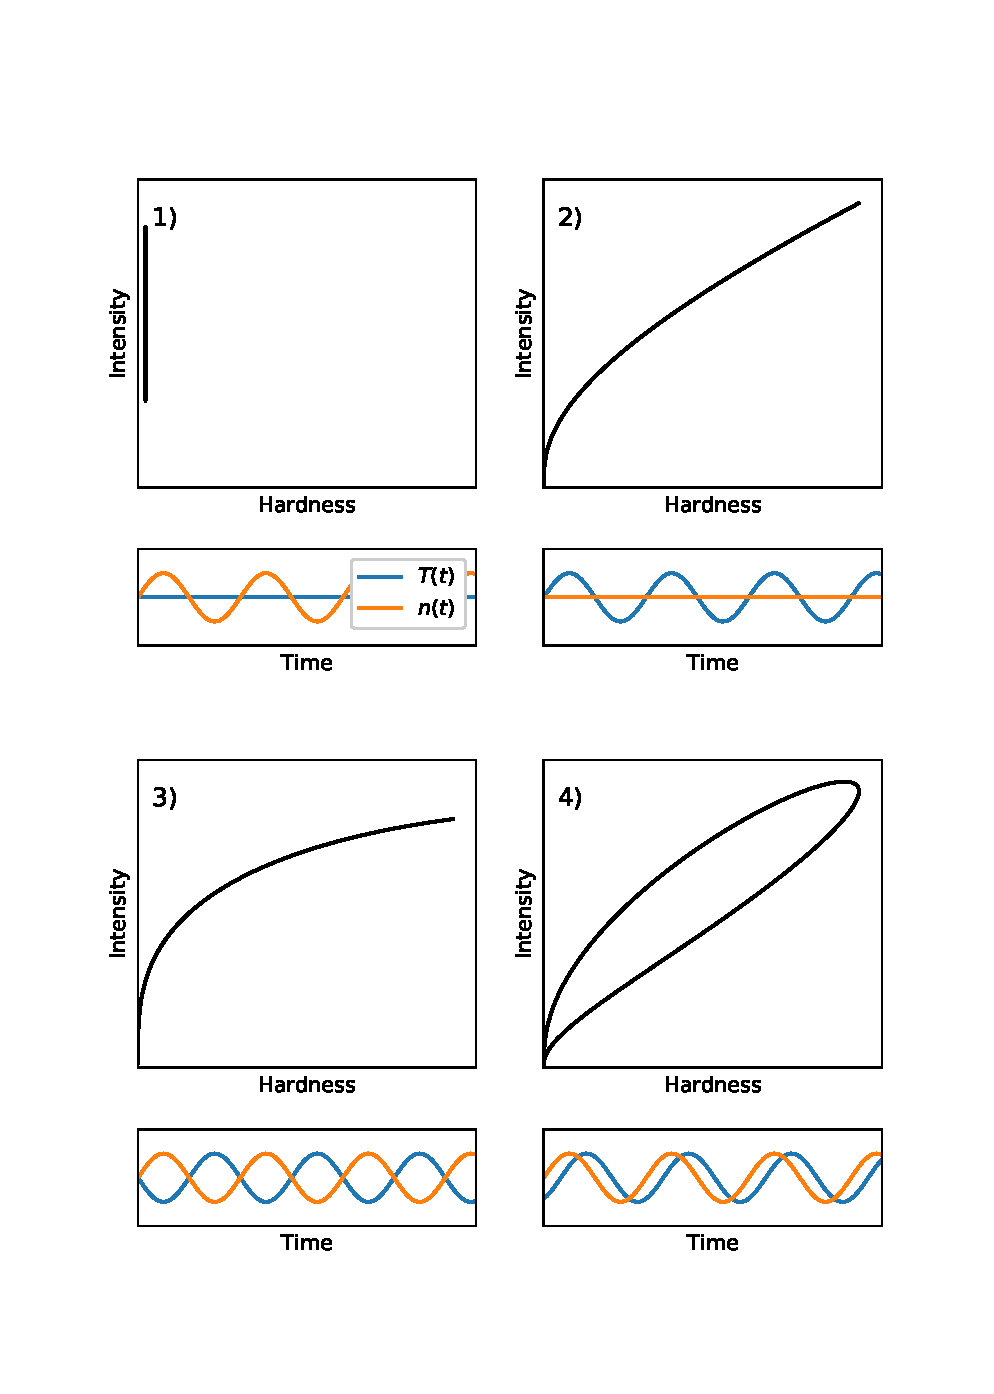
\includegraphics[width=\columnwidth, trim = 0mm 25mm 0mm 25mm]{images/hidexp.eps}
    \captionsetup{singlelinecheck=off}
    \caption[Hardness-Intensity diagrams of black bodies with temperatures and normalisations described by various functional forms.]{Hardness-Intensity diagrams of black bodies with temperatures and normalisations described by various functional forms $T(t)$ and $n(t)$.  The plots show how HIDs differ between sources with \textbf{1)} changing brightness but no spectral change, \textbf{2)} changing temperature, \textbf{3)} changing temperature and normalisation in antiphase, and \textbf{4)} changing temperature and normalisation out of phase.}
   \label{fig:HIDexp}
\end{figure}
\item $T(t)=\sin(t), n(t)=1$: in this example, the spectrum of the source changes over time, resulting in a curved track in hardness-intensity space (Figure \ref{fig:HIDexp}, Panel 2).
\item $T(t)=\sin(t), n(t)=\sin(t-\pi)$: if two or more spectral parameters are varying at once, the track can become move complex.  If these parameters are varying in phase or antiphase, a single track is traced (Figure \ref{fig:HIDexp}, Panel 3).
\item $T(t)=\sin(t), n(t)=\sin\left(t+\frac{\pi}{3}\right)$: when parameters are varying out of phase with each other, the track of the object in a HID can take the form of a closed loop (Figure \ref{fig:HIDexp}, Panel 4).
\end{enumerate}
Case 4 is interesting, as it indicates the presence of a time lag between two or more physical components of the system.  The direction in which the loop is executed over time can be used to infer the sign of this lag.  This in turn can give constraints on the causal links between components of a system, in turn giving constraints on physical models proposed to describe them.

\subsubsection{Phase-Resolved Spectroscopy}

\label{sec:phasresspec}

\par Like lightcurves, HIDs and time-resolved spectra can be difficult to analyse when constructed from data with poor statistics.  If the source is variable in a periodic or quasi-periodic way, a modified version of the folding algorithms detailed in Section \label{sec:LCMorph} can be used to analyse the spectral evolution of an average cycle:
\begin{itemize}
\item Obtain the function $\phi(t)$ to describe how phase varies as a function of time.
\item Split the interval $[0,1)$ into a number of sub-intervals $i$.
\item For each sub-interval $i$, compile a list of good time indices (GTIs) denoting periods of time during which $\phi(t)\in i$.
\item For each list of GTIs, filter the original dataset such that it only contains photons which arrived during one of the intervals.
\item From each new filtered dataset, a spectrum or hardness ratio can be calculated.  This can be compared with the spectra or hardness ratios taken from the other filtered datasets to analyse how the spectrum of the source varies as a function of phase.
\end{itemize}





\cleardoublepage

\chapter{Variability in IGR J17091-3624: Classification}

\label{ch:IGR}

\epigraph{\textit{Song and call are useful aids to identification, and reference is made to vocalisation for each species.}}{Paul Sterry -- \textit{Collins Guide to British Birds}}

\vspace{1cm}

\par\noindent Accounting for the unusual X-ray variability observed in LMXBs is required for a complete understanding of the physics of matter in their accretion disks.  The first step is to describe and categorise the types of variability in these objects, and to look for similarities and differences which may shed light on their physical origins.
\par In 2000, \citeauthor{Belloni_GRS_MI} performed a complete model-independent analysis of variability classes in GRS 1915.  This work highlighted the breadth and diversity of variability in GRS 1915, and allowed these authors to search for features common to all variability classes.  For example, \citet{Belloni_GRS_MI} found that every variability class can be expressed as a pattern of transitions between three quasi-stable phenomenological states.
\par Previous works have noted that some of the variability classes seen in IGR J17091-3624 appear very similar to those seen in GRS 1915 (e.g. \citealp{Altamirano_IGR_FH, Zhang_IGR}).  However, although $\rho$-like classes in the two objects both show lags between hard and soft X-rays photons, these lags appear to possess different signs \citep{Altamirano_IGR_FH}.  Additionally, at least two variability classes have been reported in IGR J17091 which have not yet been reported in GRS 1915 \citep{Pahari_IGRClasses}.  Previous works have described some of the behaviour seen in IGR J17091 in the context of the variability classes described by \citealt{Belloni_GRS_MI} for GRS 1915 (e.g. \citealp{Altamirano_IGR_FH,Pahari_RhoDiff}).  To further explore the comparison between GRS 1915 and IGR J17091, here I perform the first comprehensive model-independent analysis of variability classes in IGR J17091 using the complete set of \rxte\ data taken of the 2011-2013 outburst of the object.  I also use data from all other X-ray missions that observed the source during this time to analyse the long-term evolution of the outburst.

\section{Data and Data Analysis}

\label{sec:dex}

\par In this chapter, I report data from \rxte , \textit{INTEGRAL}, \textit{Swift}, \textit{Chandra}, \textit{XMM-Newton} and \textit{Suzaku} covering the 2011-2013 outburst of IGR J17091.  Unless stated otherwise, all errors are quoted at the 1$\sigma$ level.
\par In Figure \ref{fig:allmissions} I present long-term lightcurves from \rxte ,  \textit{INTEGRAL} and \textit{Swift} to show the behaviour of the source during this outburst.  I indicate when during the outburst \textit{Chandra}, \textit{XMM-Newton} and \textit{Suzaku} observations were made.

\begin{figure}
    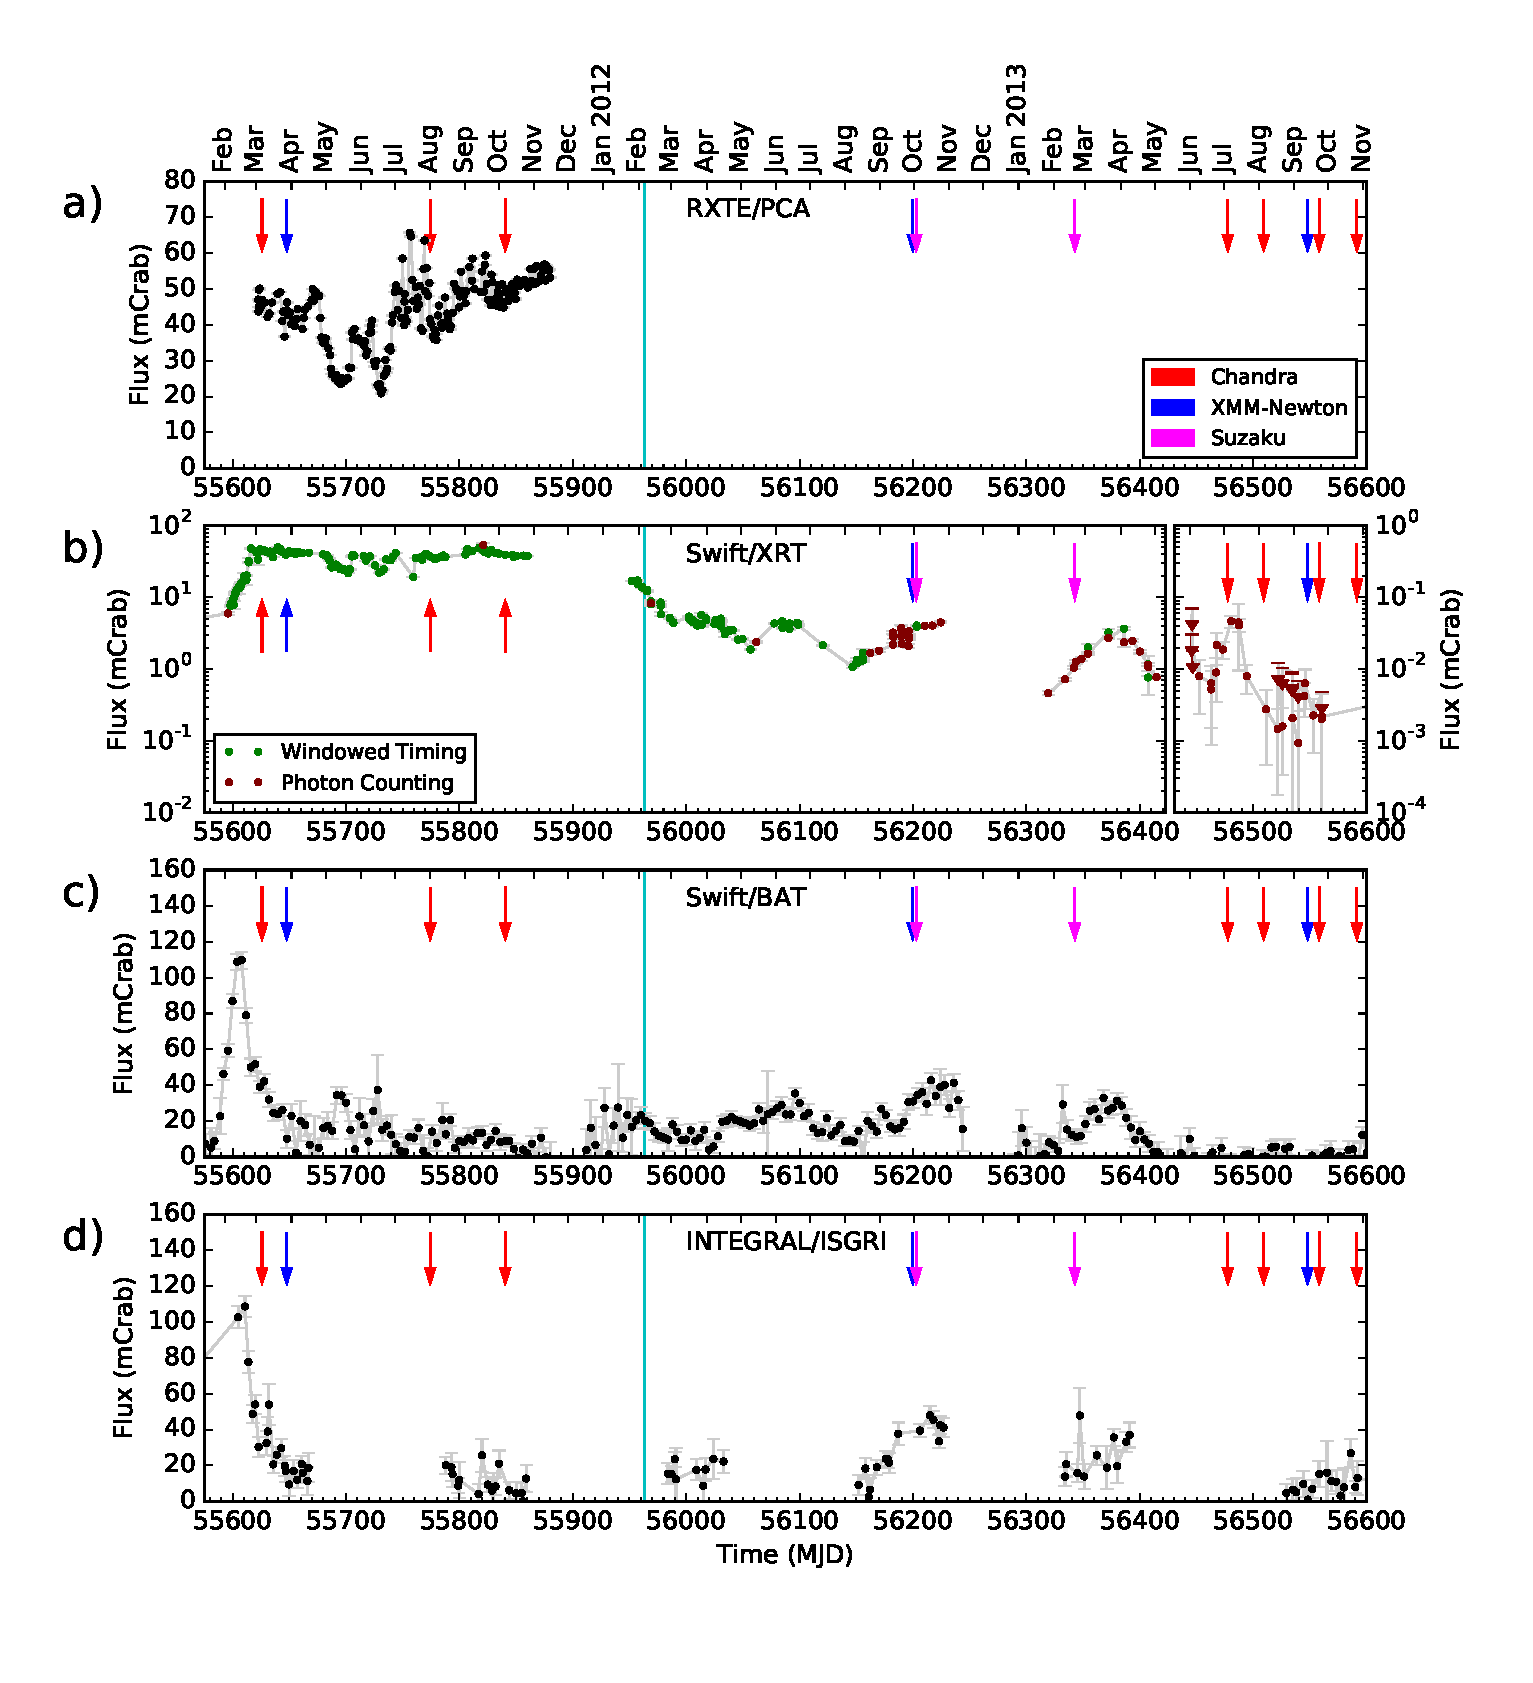
\includegraphics[width=\columnwidth, trim = {0.75cm 1.0cm 1.0cm 0.8cm},clip]{images/allmis.eps}
    \captionsetup{singlelinecheck=off}
    \caption[Lightcurves of IGR J17091-3624, from a number of instruments, during its 2011-2013 outburst.]{\rxte\ (Panel a), \textit{Swift/XRT} (Panel b), \textit{Swift/BAT} (Panel b) and \textit{INTEGRAL}/IBIS (Panel d) lightcurves of IGR J17091-3624 during its 2011-2013 outburst.  Arrows mark times at which \textit{XMM-Newton} (blue), \textit{Chandra} (red) or \textit{Suzaku} (magenta) observed IGR J17091-3624.  The cyan line represents MJD 55963, the approximate time IGR J17091-3624 transitions from the soft to the hard state \citep{Drave_Return}.  \rxte \textit{/PCA} \citep{Jahoda_PCA} data are for the 2--16\,keV energy band and taken from \citep{Altamirano_IGR_FH}, \textit{Swift/BAT} \citep{Barthelmy_BAT} data are for 15--50\,keV, \textit{Swift/XRT} \citep{Burrows_XRT}  data are for 0.3--10\,keV and \textit{INTEGRAL/ISGRI} \citep{Ubertini_IBIS} data are for 20-40\,keV.  Note that the data from \textit{Swift/XRT} (Panel B) are shown with a logarithmic $y$-axis to better show the late time progression of the outburst.  Data points are coloured according to the observing mode used.  The \textit{Swift/XRT} data from times later than MJD 56422 are shown to a different scale to better represent the post-outburst evolution of the source.  All data are presented in 1 day bins, except for data from \textit{Swift/BAT} which is presented in 4 day bins.  See also Figure \ref{fig:WhereCls}, in which data from \rxte \textit{/PCA} is presented on a smaller scale.  The Crab count rates used to normalise these data were 2300 cts s$^{-1}$ PCU$^{-1}$, 747.5 cts s$^{-1}$, 0.214 cts s$^{-1}$ and 183.5 cts s$^{-1}$ for \rxte , \textit{Swift/XRT}, \textit{Swift/BAT} and \textit{INTEGRAL/ISGRI} respectively.  \rxte\ data have not been corrected for the 25' offset to avoid contamination from GX 349+2, and for all instruments \textsf{D.A.} and I implicitly assume that IGR J17091 presents a Crab-like spectrum.}
   \label{fig:allmissions}
\end{figure}

\subsection{\rxte}

\label{sec:XTEDA}

\par For this variability study, I focus on the data from \textit{RXTE}/PCA.  I analysed all PCA observations of IGR J17091 during 2011, corresponding to ObsIDs 96065-03, 96103-01 and 96420-01.  The observations taken for proposals 96065-03 and 96103-01 were contaminated by the nearby X-ray source GX 349+2 \citep{Altamirano_IGR_FH,Rodriguez_Contamination}.  As such I only use observations performed for proposal 96420-01, corresponding to a total of 243 orbits from 215 separate observations.  These were offset by 25' such that GX 349+2 was not in the $1^\circ$ \textit{PCA} field of view.  \rxte\ was decommissioned during a period of Sun constraint centred on MJD 55907,  and hence the last observation of IGR J17091 was taken on MJD 55879.
\par I extracted data from the native \texttt{FITS} format using my own \texttt{PANTHEON} software (presented in Appendix \ref{app:PAN}).  To perform medium- to high-frequency ($\gtrsim1$\,Hz) timing analysis, I merged files formatted in PCA's `Good Xenon' data mode and extracted their data at the maximum time resolution ($\sim9.5\times10^{-7}$ s) without accounting for the background.  I divided these data into 128\,s segments as this allowed us to reach frequencies below $\sim0.015$\,Hz, partly sampling the high amplitude quasi-periodic flaring behaviour seen in many classes.  Using the Fast Fourier Transform (FFT), I produced the power spectrum of each segment separately.  I then averaged these spectra to create a one co-added Power Density Spectrum (PDS) for each observation.
\par For low-frequency ($\leq1$\,Hz) timing and correlated spectral/timing analysis, I rebinned the data to 0.5\,s and normalised count rates by the number of proportional counters (PCUs) active in each observation.  My choice of 1\,Hz allows us to analyse high amplitude `flaring' behaviour (seen at frequencies $\lesssim0.5$\,Hz) separately from the lower-amplitude behaviour seen at $\gtrsim5$\,Hz.
\par I split the data into three energy bands: A (\textit{PCA} channels 0--14, $\sim2$--$6$\,keV), B (\textit{PCA} channels 15--35, $\sim6$--$16$\,keV) and C (\textit{PCA} channels 36--255, $\sim16$--$60$\,keV).  I chose these energy bands to be consistent with the energy bands used by the model-independent classification of variability classes of GRS 1915 in \citet{Belloni_GRS_MI}.  For each of the energy-filtered lightcurves produced I estimated background using \texttt{pcabackest} from the \texttt{FTOOLS} package \citep{Blackburn_FTools} with the \textit{PCA} faint source background model\footnote{\url{http://heasarc.gsfc.nasa.gov/FTP/xte/calib\_data/pca\_bkgd/Faint/pca\_bkgd\_cmfaintl7\_eMv20051128.mdl}}. In all observations, I found that counts in the C band were consistent with background.  I then created Lightcurves $L_A$ and $L_B$ from background-subtracted photons counted in the A and B bands respectively.  I used these lightcurves to define the full-band lightcurve ($L_T=L_A+L_B$) and the soft colour ($C_1=L_B/L_A$) of each observation.  To complement the Fourier spectra, I also constructed Generalised Lomb-Scargle Periodograms of $L_T$ from each dataset, a modified version of the standard Lomb-Scargle periodogram \citep{Lomb_LombScargle, Scargle_LombScargle} that takes into account errors in the dataset \citep{Irwin_LombScargle}.  Using the Lomb-Scargle periodogram instead of the Fourier periodogram here allows us to sample the low-frequency behaviour of lightcurves with data gaps.  This is important, for example, in lightcurves which show two populations of flares, as it allows each population to be studied independently by cropping the other from the lightcurve.
\par I also used data from \citealt{Altamirano_IGR_FH} to sample the long-term colour evolution of IGR J17091.  I use 2 hardness ratios defined by \citeauthor{Altamirano_IGR_FH}: $H_{A1}$ and $H_{A2}$, corresponding to the ratios of the 2--3.5\,keV band against the 3.5--6\,keV band and the 6--9.7\,keV band against the 9.7--16\,keV band respectively.
\par When possible, if low-frequency peaks were present in the Lomb-Scargle spectrum of an observation, I used the position of the highest peak to define a value for a period.  This period was then used to fold the data to search for reccurent hysteretic patterns in the hardness-Intensity diagram (hereafter HID$_1$, a plot of $L_T$ against $C_1$).  I found that quasi-periodic oscillations in the observations I used tended to show significant frequency shifts on timescales shorter than the length of the observations.  As such, I employed the variable-period folding algorithm outlined in Section \ref{sec:Flares} where appropriate.  For cases in which this algorithm was not appropriate, I considered small sections of each lightcurve, with a length equivalent to small number of periods, before performing folding.
\par Additionally, in observations which showed a pattern of high-amplitude X-ray flaring in $L_T$, I used my own algorithm to find individual flares (this algorithm is described in Section \ref{sec:Flares}) and collect statistics on the amplitude, duration and profile of these events.
\par A list of all observations used in this study can be found in Appendix \ref{app:Obsids}.

\subsection{\textit{Swift}}

\par IGR J17091-3624 was observed with \textit{Swift}/XRT for a total of 172 pointed XRT observations between MJDs 55575 and 56600, corresponding to Target IDs 31921, 34543, 30967, 30973, 31920, 35096, 67137, 81917, 522245, 677582 and 677981.  These observations were interrupted during sun constraints centred on MJDs 55907 and 56272.  I created a long-term 0.3--10\,keV \textit{Swift/XRT} light curve, with one bin per pointed observation, using the online light-curve generator provided by the UK Swift Science Data Centre (UKSSDC; \citealp{Evans_Swift1}).  I have also created a long-term 15--50\,keV lightcurve using the publicly available \textit{Swift/BAT} daily-averaged lightcurve\footnote{\url{http://swift.gsfc.nasa.gov/results/transients/weak/IGRJ17091-3624/}}.  These are shown in Figure \ref{fig:allmissions} Panels (b) and (c) respectively.

\subsection{\textit{INTEGRAL}}

\par Dr. Chris Boone (\textsf{C.B.}) and I analyse all available observations of IGR J17091 with \textit{INTEGRAL}/IBIS \citep{Ubertini_IBIS} between MJD 55575--55625 where the source is less than 12 degrees from the centre of the field of view and where there is more than 1\,ks of good ISGRI time per 2\,ks Science Window. This corresponds to the spectrally hardest period of the 2011-2013 outburst. The filtering of observations results in a total of 188 Science Windows which were processed using the Offline Science Analysis (OSA) software version 10.2 following standard data reduction procedures\footnote{http://www.isdc.unige.ch/integral/analysis} in four energy bands (20--40, 40--100, 100--150, 150--300\,keV). These bands were selected as they are standard energy bands used in the surveys of \citet{Bird_Survey} and \citet{Bazzano_Survey} and allow comparison to these previous works. Images were created at the Science Window level, as well as a single mosaic of all Science Windows in each energy band.

\subsection{\textit{XMM-Newton}}
\label{sec:xmmdata}

\par \textit{XMM/Newton} observed IGR J17091 thrice during the period from 2011--2013 (represented by the blue arrows in Figure \ref{fig:allmissions}).  One of these observations (ObsID 0721200101) was made on 12 September 2013; I do not consider this observation further as IGR J17091 had returned to quiescence by this time \citep{Altamirano_Quiescence}.  The remaining two observations, corresponding to ObsIDs 0677980201 and 0700381301 respectively, were taken on March 27 2011 (MJD 55647) and September 29 2012 (MJD 56199).
\par During observation 0677980201, \textit{EPIC-pn} was operating in burst mode and \textit{EPIC-MOS} was operating in timing mode.  Given the low efficiency of burst mode, I only consider data from \textit{EPIC-MOS} for this observation.  During observation 0700381301, \textit{EPIC-pn} was operating in timing mode, and thus I use data from \textit{EPIC-pn} for this observation.
\par I used the \textit{XMM-Newton} Science Analysis Software version 15.0.0 (\texttt{SAS}, see \citealp{Ibarra_sas}) to extract calibrated event lists from \textit{EPIC} in both observations.  I used these to construct lightcurves to study the X-ray variability, following standard analysis threads\footnote{\url{http://www.cosmos.esa.int/web/xmm-newton/sas-threads}}.

\subsection{\textit{Chandra}}

\par \textit{Chandra} made 7 observations of IGR J17091 during the period 2011--2013.  Four of these observations were taken after IGR J17091 returned to quiescence, and I do not consider these further in this chapter.  The Chandra observations log is reported in Table \ref{tab:Chandra}. 

\begin{table}
\centering
\begin{tabular}{lllllll}
\hline
\hline
\scriptsize ObsID &\scriptsize  Instrument &\scriptsize Grating &\scriptsize Exposure (ks) &\scriptsize  Mode &\scriptsize MJD\\
\hline
12505  	& \textit{HRC-I}    &   NONE      &    1.13      & $I$ & 55626\\
12405  	& \textit{ACIS-S} &   HETG     &    31.21     & $C$ & 55774\\
12406  	& \textit{ACIS-S} &   HETG     &    27.29     & $T$ & 55840\\
\hline
\hline
\end{tabular}
\caption[\textit{Chandra} observations log covering the three observations considered in this chapter.]{\textit{Chandra} observations log covering the three observations considered in this chapter.  $I$ refers to Imaging mode, $C$ refers to CC33\_Graded mode and $T$ refers to Timed Exposure Faint mode.  HETG refers to the High Energy Transmission Grating.}
\label{tab:Chandra}
\end{table}

\par Dr. Margarita Pereyra (\textsf{M.P.}) analysed these data using \texttt{CIAO} version 4.8 \citep{Fruscione_Ciao}, following the standard analysis threads. In order to apply the most recent calibration files (CALDB 4.7.0, \citealp{Graessle_ChaCALDB}), \textsf{M.P.} reprocessed the data from the three observations using the \texttt{chandra\_repro} script\footnote{See e.g. \url{http://cxc.harvard.edu/ciao/ahelp/chandra_repro.html}}, and used this to produce data products following standard procedures.
\par The first Chandra observation (ObsID 12505) of this source was made shortly after it went into outburst in February 2011. It was a 1\,ks observation performed to refine the position of the X-Ray source, using the High-Resolution Camera in Imaging mode (HRC-I). \textsf{M.P.} created the 0.06--10\,kev light curve accounting for the Dead Time Factor (DTF), to correct the exposure time and count rate using the \texttt{dmextract} tool in the \texttt{CIAO} software.
\par Two additional observations (ObsIDs 12405 and 12406) were performed within 214 days of this first observation, using the High Energy Transmition Grating Spectrometer (HETGS) on board \textit{Chandra}. The incident X-Ray flux was dispersed onto \textit{ACIS} using a narrow strip array configuration (ACIS-S). Continuous Clocking and Time Exposure modes were use in each observation respectively (see \citealp{King_IGRWinds} for further details). \textsf{M.P.} excluded any events below 0.4\,keV, since the grating efficiency is essentially zero below this energy. In the case of the ObsID 12405 observations MP also excluded the Flight Grade 66 events in the event file, as they were not appropriately graded. \textsf{M.P.} extracted the 0.5-10\,kev HEGTS light curves, excluding the zeroth-order flux, adopting standard procedures.

\subsection{\textit{Suzaku}}

\par \textit{Suzaku} observed IGR J17091 twice during the period 2011--2013; a 42.1\,ks observation on October 2--3, 2012 (MJD 56202--56203, ObsID: 407037010) and an 81.9\,ks observation on February 19--21, 2013 (MJD 56342--56344, ObsID: 407037020). \textit{XIS} consists of four X-ray CCDs (\textit{XIS} 0, 1, 2 and 3), and all them except for XIS 2 were operating in the 1/4 window mode which has a minimum time resolution of 2 seconds.
\par Professor Kazutaka Yamaoka (\textsf{K.Y.}) analysed the \textit{Suzaku} data using {\it HEASOFT} 6.19 in the following standard procedures after reprocessing the data with \texttt{aepipeline} and the latest calibration database (version 20160607).  \textsf{K.Y.} extracted \textit{XIS} light curves in the 0.7--10 keV range, and subtracted background individually for XIS 0, 1 and 3 and then summed these to obtain the total background.  \textsf{K.Y.} created Power density spectra (PDS) using {\tt powspec} in the {\tt XRONOS} package.

\section{Results}
\label{sec:results}

\subsection{Outburst Evolution}

\label{sec:igrobevo}

\par The onset of the 2011-2013 outburst of IGR J17091 can be seen in the \textit{Swift/BAT} lightcurve (Figure \ref{fig:allmissions} Panel c).  In a 22 day period between MJDs 55584 and 55608, the 15--50\,keV intensity from IGR J17091 rose from $\sim9$\,mCrab to a peak of $\sim110$\,mCrab.  This onset rise in intensity can also be seen in 0.3--10\,keV \textit{Swift/XRT} data and 20--40\,keV \textit{INTEGRAL/ISGRI} data.
\par After peak intensity, the 15--50\,keV flux (\textit{Swift/BAT}) began to steadily decrease, until returning to a level of $\sim$20\,mCrab by MJD 55633.  A similar decrease in flux can be seen in the data obtained by \textit{INTEGRAL} at this time (Figure \ref{fig:allmissions} Panel (d).  However, there was no corresponding fall in the flux at lower energies; both the long-term 2--16\,keV \rxte\ data and \textit{Swift/XRT} data (Panels a and b respectively) show relatively constant fluxes of 45\,mCrab between MJDs 55608 and 55633.
\par The significant decrease in high-energy flux during this time corresponds to IGR J17091 transitioning from a hard state to a soft intermediate state \citep{Pahari_RhoDiff}.  This transition coincides with a radio flare reported by \citet{Rodriguez_D} which was observed by the Australian Telescope Compact Array (\textit{ATCA}).
\par \citealp{Altamirano_10Hz} first reported a 10\,mHz QPO in \rxte\ data on MJD 55634 , evolving into `Heartbeat-like' flaring by MJD 55639 \citep{Altamirano_Discovery}.  Between MJDs 55634 and 55879, the global \rxte\ lightcurve shows large fluctuations in intensity on timescales of days to weeks, ranging from a minimum of $\sim1$\,mCrab on MJD 55731 to a maximum of $\sim66$\,mCrab on MJD 55756.  The \textit{Swift/XRT} lightcurve shows fluctuations that mirror those seen by \rxte\ during this period, but the amplitude of the fluctuations is significantly reduced.
\par \textit{Swift/XRT} was unable to observe again until MJD 55952.  Between this date and MJD 55989, \textit{Swift/XRT} observed a gradual decrease in intensity corresponding to a return to the low/hard state \citep{Drave_Return}.
\par Between MJD 55989 and the end of the outburst on MJD 56445, there are secondary peaks in the \textit{Swift/XRT}, \textit{Swift/BAT} and \textit{INTEGRAL/ISGRI} lightcurves that evolve over timescales of $\lesssim100$ days.  Similar humps have been seen before in lightcurves from other objects, for example the black hole candidate XTE J1650-500 \citep{Tomsick_MiniOutbursts} and the neutron stars SAX J1808.4-3658 \citep{Wijnands_1808} and SAX J1750.8-2900 \citep{Allen_1750}.  These humps are referred to as `re-flares' (also as `rebrightenings',  `echo-outbursts', `mini-outbursts' or a `flaring tail', e.g. \citealp{Patruno_Reflares2}).  I identify a total of 3 apparent re-flares in the \textit{Swift/BAT} data, centred approximately at MJDs 56100, 56220 and 56375.
\par The observation with \textit{XMM-Newton/EPIC-pn} on MJD 56547 (12 September 2013) recorded a rate of 0.019 cts s$^{-1}$.  An observation with \textit{EPIC-pn} in 2007, while IGR J17091 was in quiescence \citep{Wijnands_Quiescence}, detected a similar count rate of 0.020 cts s$^{-1}$.  Therefore I define MJD 56547 as the upper limit on the endpoint of the 2011-2013 outburst.  As such the outburst, as defined here, lasted for $\lesssim$952 days.
\par After the end of the 2011-2013 outburst, IGR J17091 remained in quiescence until the start of a new outburst around MJD 57444 (26 February 2016, \citealp{Miller_2016Outburst}).

\subsection{\rxte}

\par Using the data products described in Section \ref{sec:dex}, I assigned a model-independent variability class to each of the 243 \rxte\textit{/PCA} orbits.  To avoid bias, this was done without reference to the classes defined by \citet{Belloni_GRS_MI} to describe the behaviour of GRS 1915.
\par Classes were initially assigned based on analysis of lightcurve profiles, count rate, mean fractional RMS \citep{Vaughan_RMS}, Fourier and Lomb-scargle power spectra and hardness-intensity diagrams.  For observations with significant quasi-periodic variability at a frequency lower than $\sim1$\,Hz, I also attempted to fold lightcurves to analyse count rate and colour as a function of phase.  When flares were present in the lightcurve, I used my algorithm (described in Section \ref{sec:Flares}) to sample the distribution of parameters such as peak flare count rate, flare rise time and flare fall time.  All parameters were normalised per active PCU, and fractional RMS values were taken from 2--60\,keV lightcurves binned to 0.5\,s.  I identify nine distinct classes, labelled I to IX; I describe these in the following sections.
\par Although the criteria for assigning each class to an observation was different, a number of criteria were given the most weight.  In particular, the detection, $q$-value and peak frequency of a QPO in the range 2\,Hz--10\,Hz were used as criteria for all classes, as well as the presence or absence of high-amplitude quasi-periodic flaring with a frequency between 0.01--1\,Hz.  The folded profile of these flares, as well as the presence of associated harmonics, were also used as classification diagnostics in observations.  Additionally, the presence or absence of low count-rate 'dips' in a lightcurve was used as a criterion for Classes VI, VIII and IX.  Detailed criteria for each individual class are given below in Sections \ref{sec:ClassI} to \ref{sec:ClassIX}.
\par For hardness-intensity diagrams, I describe looping behaviour with the terms `clockwise' and `anticlockwise'; in all cases, these terms refer to the direction of a loop plotted in a hardness-intensity diagram with colour on the $x$-axis and intensity on the $y$-axis.
\par In Appendix \ref{app:Obsids}, I present a list of all orbits used in the study along with the variability classes I assigned to them.
\par In Figure \ref{fig:WhereCls}, I show global 2--16\,keV lightcurves of IGR J17091 during the 2011-2013 outburst.  In each panel, all observations of a given class are highlighted in red.  A characteristic lightcurve is also presented for each class.  In Figure \ref{fig:IIIisHarder} panel (a), I show a plot of average hardness $H_{A2}$ against $H_{A1}$ for each observation, showing the long-term hysteresis of the object in colour-colour space.  Again, observations belonging to each variability class are highlighted.  In Figure \ref{fig:IIIisHarder} panels (b) and (c), I show global hardness-intensity diagrams for $H_{A1}$ and $H_{A2}$ respectively.
\par In Figure \ref{fig:IIIisHarder} Panel (a), we see that IGR J17091-3624 traces a two branched pattern in colour-colour space corresponding to a branch which is soft ($\sim0.9$) in $H_{A1}$ and variable in $H_{A2}$ and a branch which is soft ($\sim0.5$) in $H_{A2}$ and variable in $H_{A1}$.  The `soft' HID shown in Figure \ref{fig:IIIisHarder} Panel (b) is dominated by a branch with a wide spread in $H_{A1}$ and intensities between $\sim40\mbox{--}60$\,mCrab.  A second branch exists at lower intensities, and shows an anticorrelation between intensity and $H_{A1}$.  Finally, the `hard' HID shown in Figure \ref{fig:IIIisHarder} Panel (c) shows an obvious anticorrelation between $H_{A2}$ and intensity, but there is also a secondary branch between $H_{A2}\approx 0.7\mbox{--}0.9$ at a constant intensity of $\sim40$\,mCrab.

\begin{figure}
    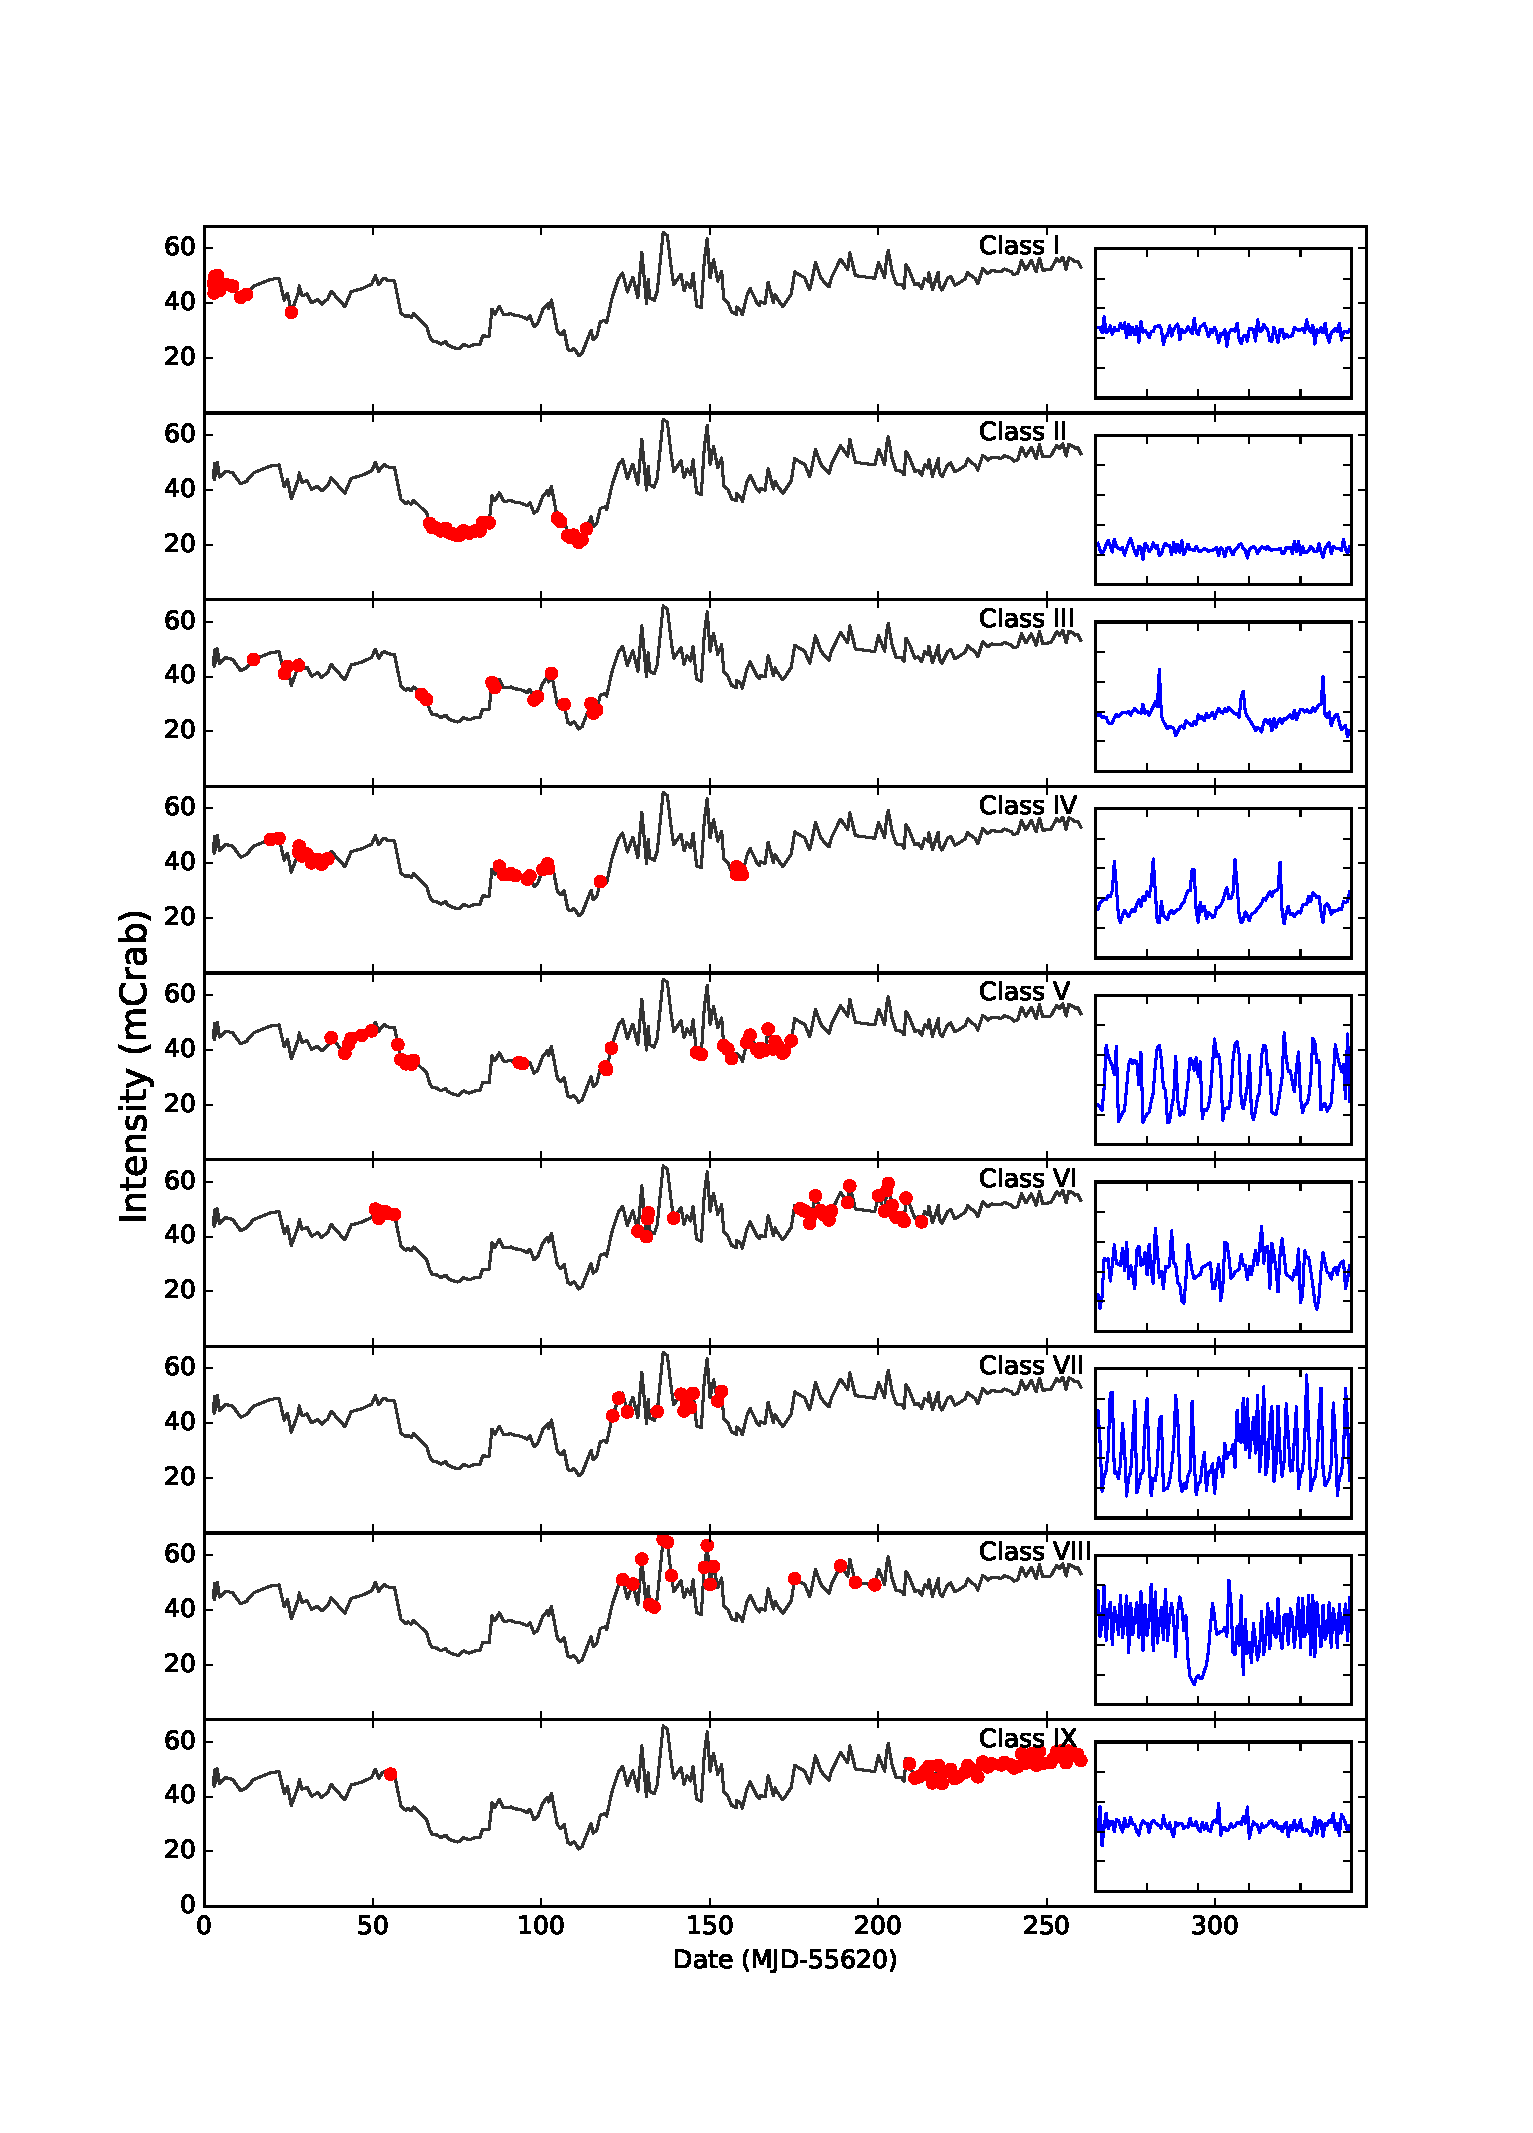
\includegraphics[width=\columnwidth, trim = {1.3cm 2.0cm 1.8cm 1.8cm},clip]{images/all_lc.eps}
    \captionsetup{singlelinecheck=off}
    \caption[Lightcurves of IGR J17091-3524 during the 2011-2013 outburst, showing when each of variability classes I-IX were observed.]{Global 2--3.5\,keV Lightcurves of IGR J17091-3524 during the 2011-2013 outburst, with each point corresponding to the mean Crab-normalised count rate of a single \rxte\ observation of the object (in turn corresponding to between 0.4 and 3.6 ks of data).  In each lightcurve, every observation identified as belonging to a particular class (indicated on the plot) is highlighted.  These are presented along with a characteristic lightcurve (inset) from an observation belonging to the relevant class.  Each lightcurve is 250\,s in length, and has a $y$-scale from 0 to 250\spcu .  Data taken from \citealt{Altamirano_IGR_FH}.}
   \label{fig:WhereCls}
\end{figure}

\begin{figure}
\centering
\subfloat[\textit{Colour-Colour Diagram}]{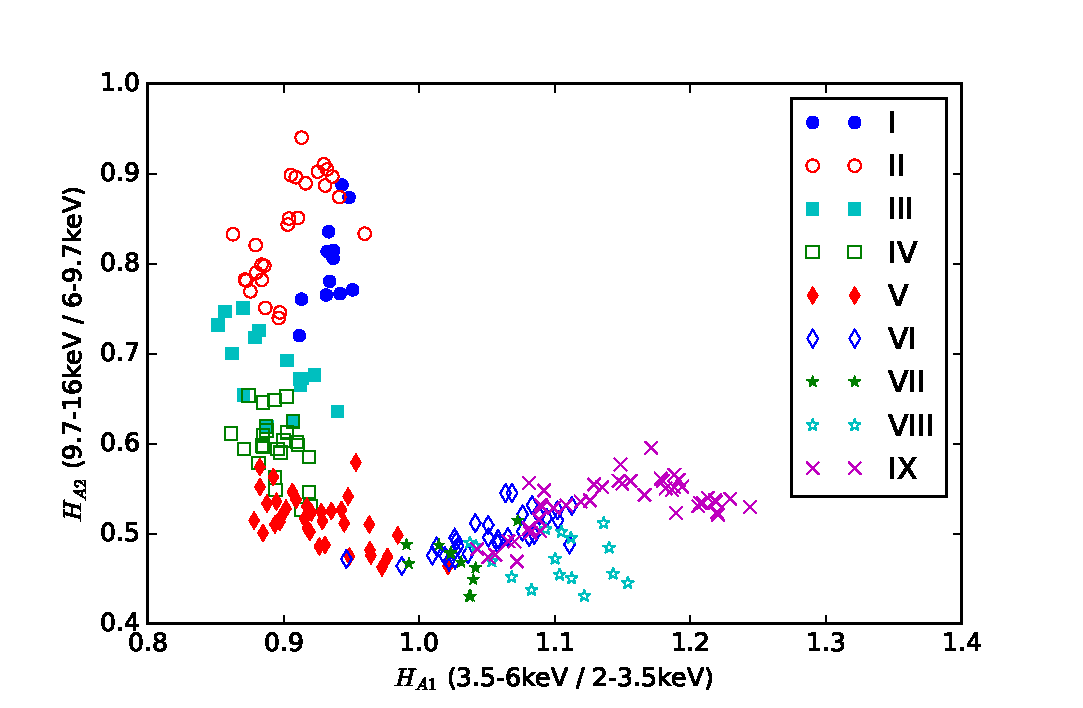
\includegraphics[width=0.8\columnwidth, trim = 0mm 0mm 0mm 8mm,clip]{images/all_ccd.eps}}\\
\subfloat[\textit{"Soft" ($H_{A1}$) Hardness-Intensity Diagram}]{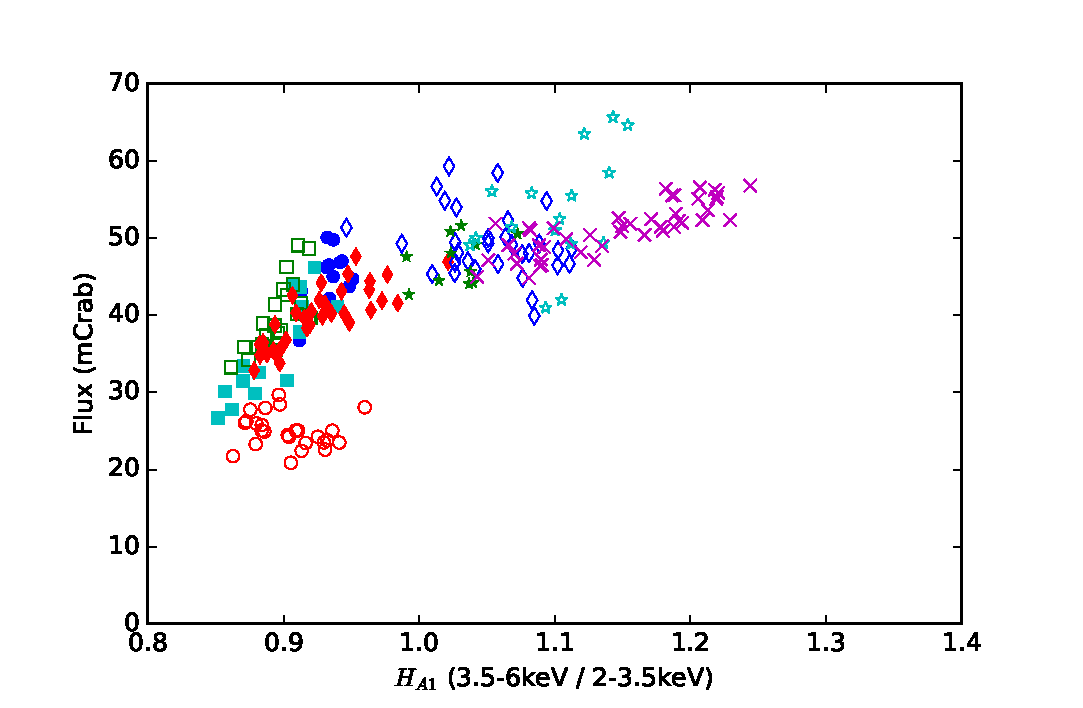
\includegraphics[width=0.8\columnwidth, trim = 0mm 0mm 0mm 8mm,clip]{images/all_shid_colorful.eps}}\\
\subfloat[\textit{"Hard" ($H_{A2}$) Hardness-Intensity Diagram}]{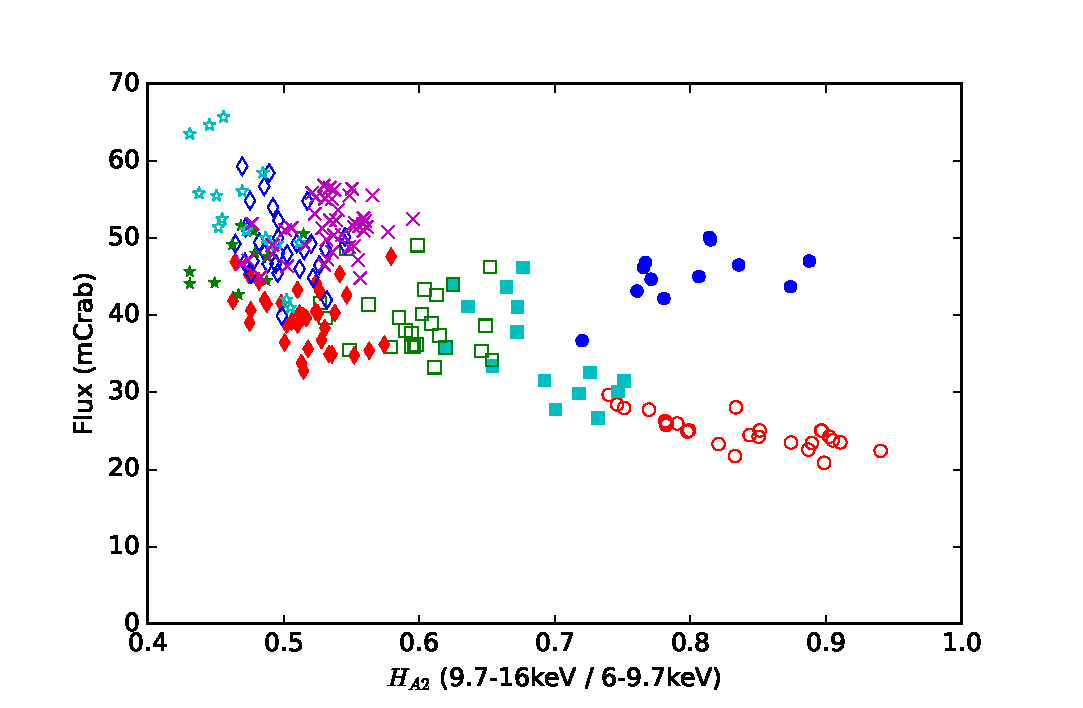
\includegraphics[width=0.8\columnwidth, trim = 0mm 0mm 0mm 8mm,clip]{images/all_hhid_colorful.eps}}\\
\captionsetup{singlelinecheck=off}
\caption[Hardness-Intensity diagrams of IGR J17091-3524 during the 2011-2013 outburst, showing when each of variability classes I-IX were observed.]{A global colour-colour diagram (a), "soft" hardness-intensity diagram (b) and "hard" hardness-intensity diagram (c) of the 2011-2013 outburst of IGR J17091, using the colours $H_{A1}$ and $H_{A2}$ defined previously.  Observations belonging to different classes have been highlighted in different colours.  Data taken from \citealt{Altamirano_IGR_FH}.}
\label{fig:IIIisHarder}
\end{figure}

\par For characteristic count rates and colours in each class, I quote the upper and lower quartile values \citep{Kenney_Quartile} instead of the mean.  This is due to the presence of high-amplitude but short-lived flares in many of the classes I describe.  Using the upper and lower quartiles as my measure of average and distribution means that my values will be less susceptible to outlier values of count rate and colour present in these flares.  All count rates have been background corrected (see Section \ref{sec:XTEDA}).
\par I have obtained mean values for these count rate quartiles, as well as values for colour $C_1$ and fractional RMS, by calculating these values individually for each orbit.  Histograms were then constructed from these datasets for each class, such that the mean and standard deviation of these values could be measured for each class.  These values are presented in Table \ref{tab:basicparams}.
\par I describe QPOs in terms of their $q$-value; a measure of coherence defined by the ratio of peak frequency and full-width half-maximum of each QPO.  I collected these values by fitting my power spectra with Lorentzians.

\begin{table}
\centering
\begin{tabular}{rllll} % four columns, alignment for each
\hline
\hline
\scriptsize Class &\scriptsize LQ Rate &\scriptsize  UQ Rate &\scriptsize Frac. RMS &\scriptsize Median C$_1$\\
\scriptsize &\scriptsize (cts s$^{-1}$) &\scriptsize (cts s$^{-1}$) & & \\
\hline
I&84--108&106--132&0.13--0.19&0.4--0.68\\
II&43--57&59--71&0.15--0.23&0.4--0.68\\
III&64--84&80--110&0.17-0.23&0.35--0.45\\
IV&63--81&92--122&0.27--0.37&0.32--0.4\\
V&49--67&88--134&0.44--0.54&0.28--0.46\\
VI&64--98&111--155&0.29--0.47&0.33--0.61\\
VII&65--79&128--140&0.45--0.57&0.32--0.42\\
VIII&62--88&142--178&0.42--0.52&0.36--0.49\\
IX&87--111&114--144&0.16--0.24&0.42-0.6\\
\hline
\hline
\end{tabular}
\caption[A number of statistics averaged across all observations belonging to each IGR J17091 variability class.]{Lower and upper quartile count rates, fractional RMS and median colour averaged across all observations belonging to each class.  Count rates and fractional RMS are taken from the full energy range of \rxte\textit{/PCA}, and fractional RMS values are 2--60\,keV taken from lightcurves binned to 0.5\,s.  Count rates are normalised for the number of PCUs active during each observation.  All values are quoted as $1\sigma$ ranges.}
\label{tab:basicparams}
\end{table}

\par For each class, I present three standard data products; a 500\,s lightcurve, a variable-length lightcurve where the length has been selected to best display the variability associated with the class and a Fourier PDS.  Unless otherwise stated in the figure caption, the 500\,s lightcurve and the Fourier PDS are presented at the same scale for all classes.  In Table \ref{tab:CPopD} I present a tally of the number of times I assigned each Variability Class to an \rxte\ orbit.

\begin{table}
\centering
\begin{tabular}{llll}
\hline
\hline
\scriptsize Class &\scriptsize  Orbits &\scriptsize Total Time (s) &\scriptsize Fraction \\
\hline
I & 31 &  69569 & 14.8\%\\
II & 26 &  50875 & 10.8\%\\
III & 14 &  26228 & 5.6\%\\
IV & 31 &  69926 & 14.9\%\\
V & 35 &  72044 & 15.3\%\\
VI & 29 &  54171 & 11.5\%\\
VII & 11 &  19241 & 4.1\%\\
VIII & 16 &  26553 & 5.7\%\\
IX & 50 &  81037 & 17.3\%\\
\hline
\hline
\end{tabular}
\caption[A tally of the number of times I assigned each of my nine Variability Classes to an \rxte\ orbit observing IGR J17091.]{A tally of the number of times I assigned each of my nine Variability Classes to an \rxte\ orbit.  I have also calculated the amount of observation time corresponding to each class, and thus inferred the fraction of the time that IGR J17091 spent in each class.  Note: the values in the Total Time column assume that each orbit only corresponds to a single variability Class.}
\label{tab:CPopD}
\end{table}



\subsubsection{Class I --  Figure \ref{fig:Bmulti}}
\label{sec:ClassI}

\begin{figure}
    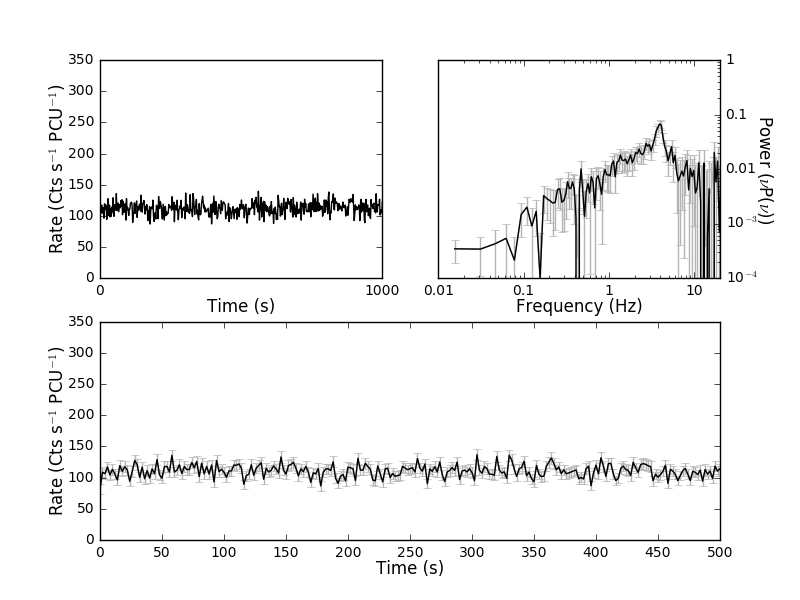
\includegraphics[width=0.8\columnwidth, trim = 0.6cm 0 3.9cm 0]{images/Bmulti.png}
    \captionsetup{singlelinecheck=off}
    \caption[Characteristic lightcurves and a power spectrum of Type I variability.]{Plots of the Class I observation 96420-01-01-00, orbit 0.  \textit{Top-left}: 1000\,s lightcurve binned on 2 seconds to show lightcurve evolution.  \textit{Top-right}: Fourier Power Density Spectrum.  \textit{Bottom}: 500\,s lightcurve binned on 2 seconds.}
   \label{fig:Bmulti}
\end{figure}

In the 2\,s binned lightcurve of a Class I observation, there is no structured second-to-minute scale variability.  The Fourier PDS of all observations in this class shows broad band noise between $\sim1$--$10$\,Hz, as well as a weak QPO (with a $q$-value of $\sim5$) which peaks at around 5\,Hz.

\subsubsection{Class II -- Figure \ref{fig:Emulti}}

\begin{figure}
    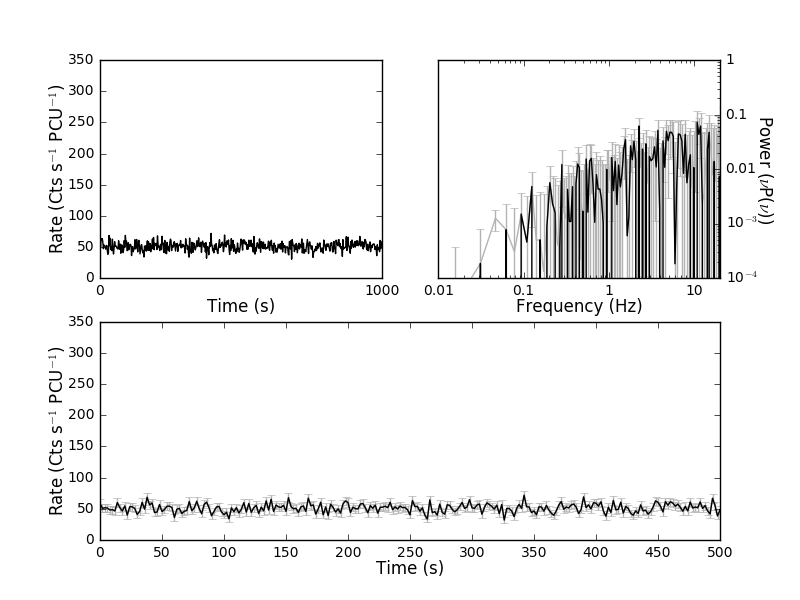
\includegraphics[width=0.8\columnwidth, trim = 0.6cm 0 3.9cm 0]{images/Emulti.png}
    \captionsetup{singlelinecheck=off}
    \caption[Characteristic lightcurves and a power spectrum of Type II variability.]{Plots of the Class II observation 96420-01-11-00, orbit 0.  \textit{Top-left}:  1000\,s lightcurve binned on 2 seconds to show lightcurve evolution.  \textit{Top-right}: Fourier Power Density Spectrum.  \textit{Bottom}: Lightcurve binned on 2 seconds.}
   \label{fig:Emulti}
\end{figure}

\par Class II observations are a factor of $\sim2$ fainter in the $L_T$ band than Class I observations.  They also occupy a different branch in a plot of hardness $H_{A2}$ against flux (see Figure \ref{fig:IIIisHarder}, panel c).  The PDS shows no significant broad band noise above $\sim1$\,Hz unlike that which is seen in Class I.  The $\sim$5\,Hz QPO seen in Class I is absent in Class II.

\subsubsection{Class III -- Figure \ref{fig:Gmulti}}
\label{sec:classIII}

\begin{figure}
    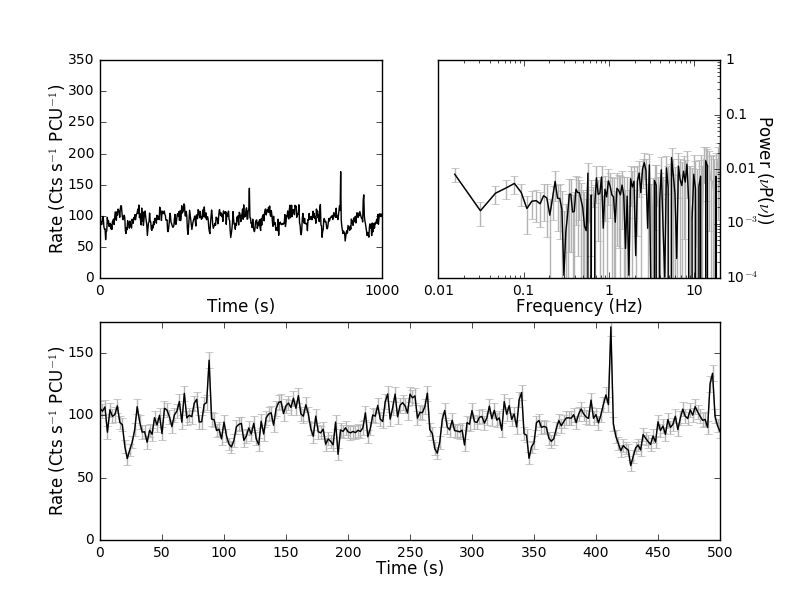
\includegraphics[width=0.8\columnwidth, trim = 0.6cm 0 3.9cm 0]{images/Gmulti.png}
    \captionsetup{singlelinecheck=off}
    \caption[Characteristic lightcurves and a power spectrum of Type III variability.]{Plots of the Class III observation 96420-01-04-01, orbit 0.  \textit{Top-left}: 1000\,s lightcurve binned on 2 seconds to show lightcurve evolution.  \textit{Top-right}: Fourier Power Density Spectrum.  \textit{Bottom}: Lightcurve binned on 2 seconds.  Note that, to emphasise the behaviour of the lightcurve in this class, I have magnified the 500\,s lightcurve y-scale by a factor of 2 compared with the lightcurves presented for other classes.}
   \label{fig:Gmulti}
\end{figure}

\par Unlike Classes I \& II, Class III lightcurves show structured flaring, with a peak-to-peak recurrence time of $42$--$80$\,s.  Most flares consist of a steady $\sim60$\,s rise in count rate and then an additional and sudden rise to a peak count rate at $\gtrsim200$\spcu which lasts for $\lesssim$0.5\,s before returning to continuum level (we have magnified the y-scaling in the lightcurve of Figure \ref{fig:Gmulti} to emphasise this behaviour). This sudden rise is not present in every flare; in some observations it is absent from every flare feature.  No 5\,Hz QPO is present in the PDS and there is no significant variability in the range between $\sim1\mbox{--}10$\,Hz.

\par As this class has a well-defined periodicity, I folded data in each observation to improve statistics using the best-fit period obtained from generalised Lomb-Scargle Periodogram Analysis; I show a representative Lomb-Scargle periodogram in Figure \ref{fig:IIILS}.  I find an anticlockwise hysteretic loop in the folded HID$_1$ of all 15 Class III orbits.  In Figure \ref{fig:LoopIII} I show an example of one of these loops.

\begin{figure}
    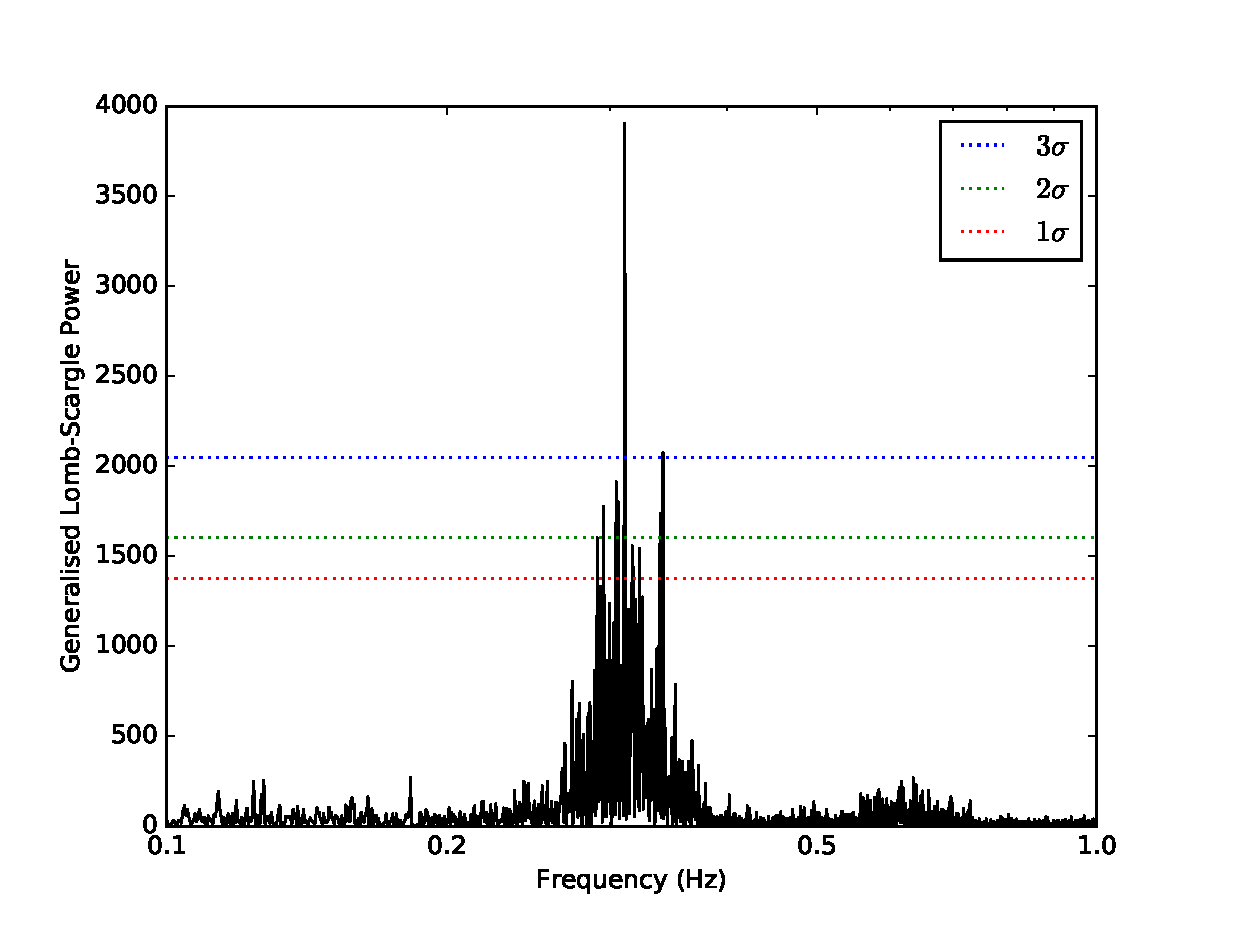
\includegraphics[width=\columnwidth, trim = 0mm 0mm 0mm 0mm]{images/LSVIII.eps}
    \captionsetup{singlelinecheck=off}
    \caption[The Lomb-Scargle periodogram of Class III observation 96420-01-19-01]{The Lomb-Scargle periodogram of observation 96420-01-19-01, orbit 0, with significance levels of 1, 2 and 3$\sigma$ plotted.  The peak at 0.31\,Hz was used to define a QPO frequency when folding the data from this observation.}
   \label{fig:IIILS}
\end{figure}

\begin{figure}
    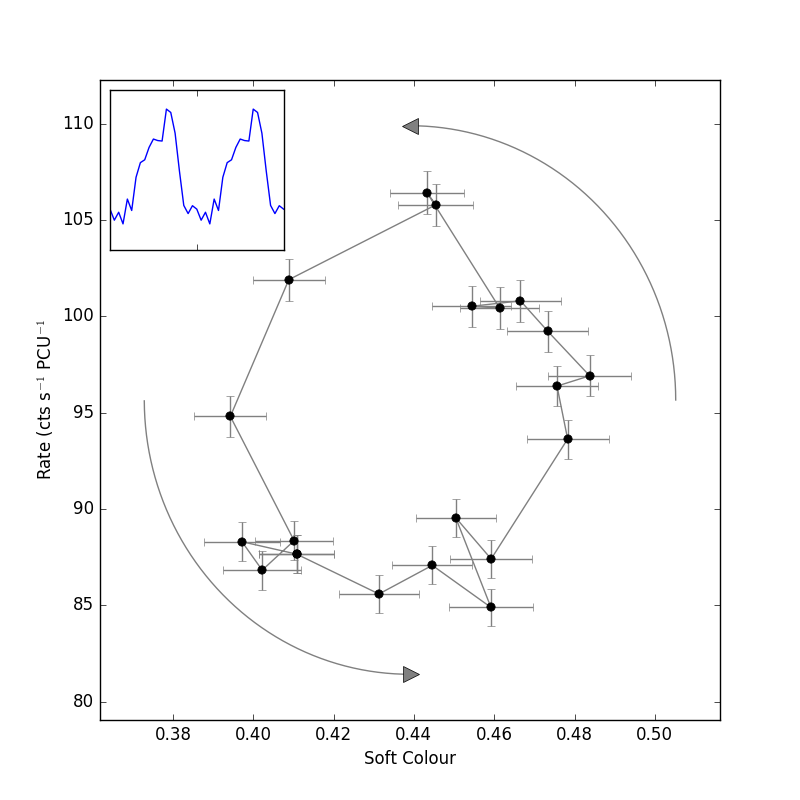
\includegraphics[width=\columnwidth, trim = 0mm 0mm 0mm 0mm]{images/Gloop.png}
    \captionsetup{singlelinecheck=off}
    \caption[A hardness-intensity diagram of the Class III observation 96420-01-04-01.]{The hardness-intensity diagram (HID$_1$) of the Class III observation 96420-01-04-01, orbit 0.  The data have been folded over a period of 79.61 s, corresponding to the peak frequency in the Lomb-Scargle spectrum of this observation.  Inset is the folded lightcurve of the same data.}
   \label{fig:LoopIII}
\end{figure}

\subsubsection{Class IV -- Figure \ref{fig:Jmulti}}
\label{sec:classIV}

\begin{figure}
    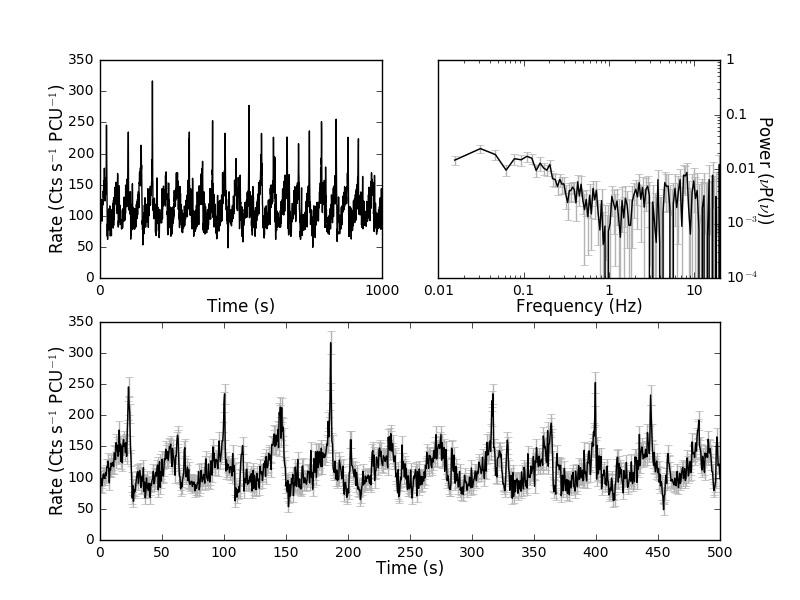
\includegraphics[width=0.8\columnwidth, trim = 0.6cm 0 3.9cm 0]{images/Jmulti.png}\\
    \captionsetup{singlelinecheck=off}
    \caption[Characteristic lightcurves and a power spectrum of Type IV variability.]{Plots of the Class IV observation 96420-01-05-00, orbit 0.  \textit{Top-left}: 1000\,s lightcurve binned on 2 seconds to show lightcurve evolution.  \textit{Top-right}: Fourier Power Density Spectrum.  \textit{Bottom}: Lightcurve binned on 0.5 seconds.}
   \label{fig:Jmulti}
\end{figure}

\par The lightcurves in this class show regular variability with a peak-to-peak recurrence time of $25$--$39$\,s.  I performed peak analysis (see Section \ref{sec:Flares}) on observations belonging to this class, finding that each peak has a rise time with lower and upper quartile values of $19.5$ and $33.5$ s, a fall time with lower and upper quartile values of $4.6$ and $13.5$\,s and a peak count rate of $159$--$241$\spcu\ .  There are no prominent significant QPOs in the Fourier PDS above $\sim1$\,Hz.
\par I folded individual Class IV lightcurves and found anticlockwise hysteretic loops in the HID$_1$ of 14 out of 30 Class IV observations.  In the top panel of Figure \ref{fig:LoopIV} I show an example of one of these loops.  However, I also find clockwise hysteretic loops in 6 Class IV observations, and in 10 orbits the data did not allow us to ascertain the presence of a loop.  I provide an example of both of these in the lower panels of Figure \ref{fig:LoopIV}.  I note that the structure of clockwise loops are more complex than anticlockwise loops in Class IV, consisting of several lobes\footnote{In HIDs with multiple lobes, the loop direction I assign to the observation corresponds to the direction of the largest lobe.} rather than a single loop (Figure \ref{fig:LoopIV}, bottom-left).

\begin{figure}
    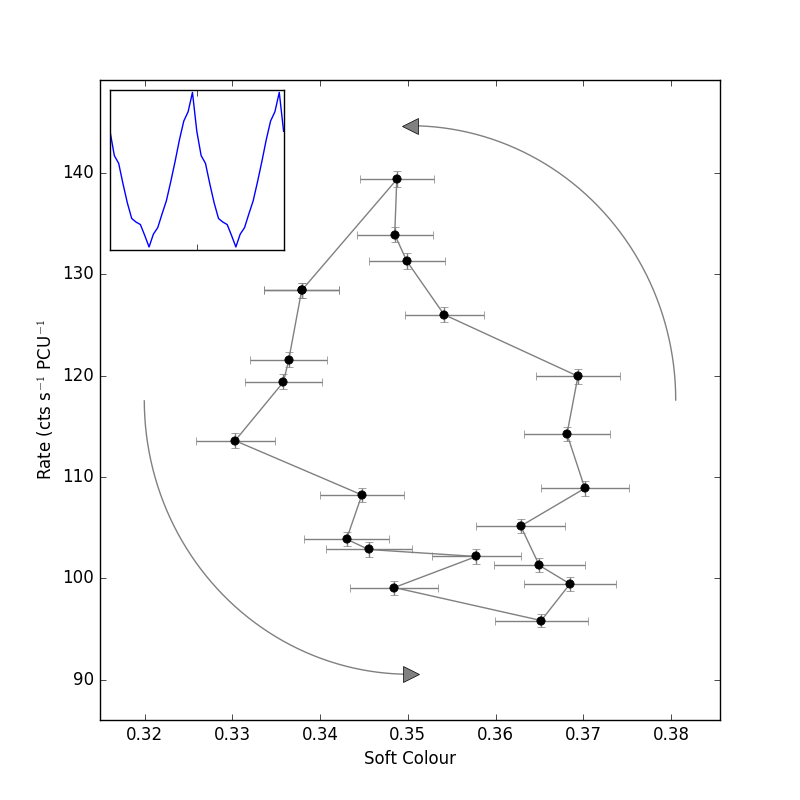
\includegraphics[width=\columnwidth, trim = 0mm 0mm 0mm 0mm]{images/Jloop.png}\\
    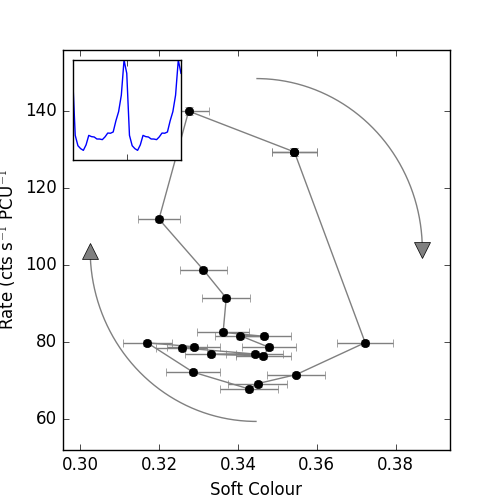
\includegraphics[width=0.5\columnwidth, trim = 0mm 0mm 0mm 0mm]{images/Jloop4.png}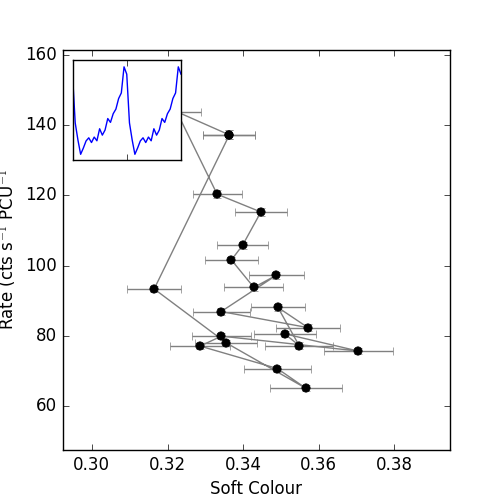
\includegraphics[width=0.5\columnwidth, trim = 0mm 0mm 0mm 0mm]{images/Jloop3.png}
    \captionsetup{singlelinecheck=off}
    \caption[The hardness-intensity diagram of the Class IV observation 96420-01-05-00, showing an anticlockwise loop.]{\textit{Top}: The hardness-intensity diagram (HID$_1$) of the Class IV observation 96420-01-05-00, orbit 0 showing an anticlockwise loop.  The data have been folded over a variable period found with the algorithm described in Section \ref{sec:Flares}.  Inset is the folded lightcurve of the same data.  \textit{Bottom Left}: The hardness-intensity diagram of Class IV observations 96420-01-24-02 orbit 0, an example of a clockwise loop.  \textit{Bottom Right}: The hardness-intensity diagram of Class IV observation 96420-01-06-00 orbit 0, in which I was unable to ascertain the presence of a loop.}
   \label{fig:LoopIV}
\end{figure}

\par Compared with Class III, the oscillations in Class IV occur with a significantly lower period, with a mean peak-to-peak recurrence time of $\sim30$\,s compared to $\sim60$\,s in Class III.
\par In Figure \ref{fig:IIIisHarder} I show that Classes III and IV can also be distinguished by average hardness, as Class III tends to have a greater value of $H_{A2}$ than Class IV.

\subsubsection{Class V -- Figure \ref{fig:Kmulti}}
\label{sec:classV}

\begin{figure}
    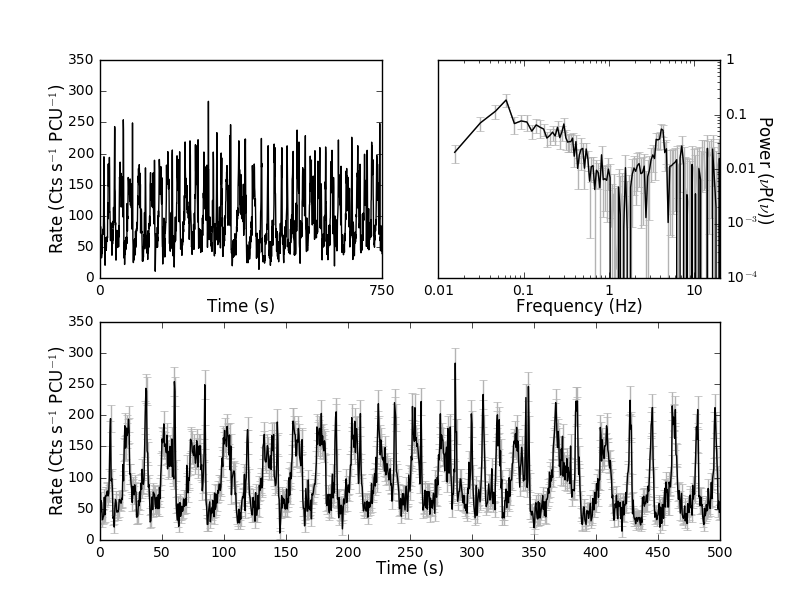
\includegraphics[width=0.8\columnwidth, trim = 0.6cm 0 3.9cm 0]{images/Kmulti.png}
    \captionsetup{singlelinecheck=off}
    \caption[Characteristic lightcurves and a power spectrum of Type V variability.]{Plots of the Class V observation 96420-01-06-03, orbit 0.  \textit{Top-left}: 750\,s lightcurve binned on 2 seconds to show lightcurve evolution.  \textit{Top-right}: Fourier Power Density Spectrum. \textit{Bottom}: Lightcurve binned on 0.5 seconds.}
   \label{fig:Kmulti}
\end{figure}

\par The lightcurves in this class, like in Classes III and IV, show flaring behaviour, with flares separated by a few tens of seconds.  At higher frequencies, the PDS shows a prominent QPO centred at $\sim4$\,Hz with as $q$-value of $\sim3$.  There is also significant broad band noise between $\sim0.1$--$1$\,Hz
\par In Figure \ref{fig:id_flares_V} I show that the flaring in this class is more complex than that seen in Classes III and IV.  Class V lightcurves consist of short strongly peaked symmetrical flares (hereafter Type $V_1$) and a longer more complex type of flare (hereafter Type $V_2$).  The Type $V_2$ flare consists of a fast rise to a local maximum in count rate, followed by a $\sim10$\,s period in which this count rate gradually reduces by $\sim50\%$ and then a much faster peak with a maximum count rate between 1 and 2 times that of the initial peak.  In both types of flare, I find that the increase in count rate corresponds with an increase in soft colour.  The two-population nature of flares in Class V can also clearly be seen in Figure \ref{fig:two_popV}, where I show a two-dimensional histogram of flare peak count rate against flare duration.
\par I folded all individual Class V lightcurves, in each case cropping out periods of $V_2$ flaring.  I find clockwise hysteretic loops in the HID$_1$ of 30 out of 33 Class V observations, suggesting a lag in the aforementioned relation between count rate and soft colour.  In the upper panel Figure \ref{fig:LoopV} I present an example of one of these loops.  In one observation however, I found an anticlockwise loop in the HID$_1$ (shown in Figure \ref{fig:LoopV} lower-left panel).  I was unable to ascertain the presence of loops in the remaining 2 orbits; for the sake of completeness, I show one of these in the lower-right panel of Figure \ref{fig:LoopV}.

\begin{figure}
    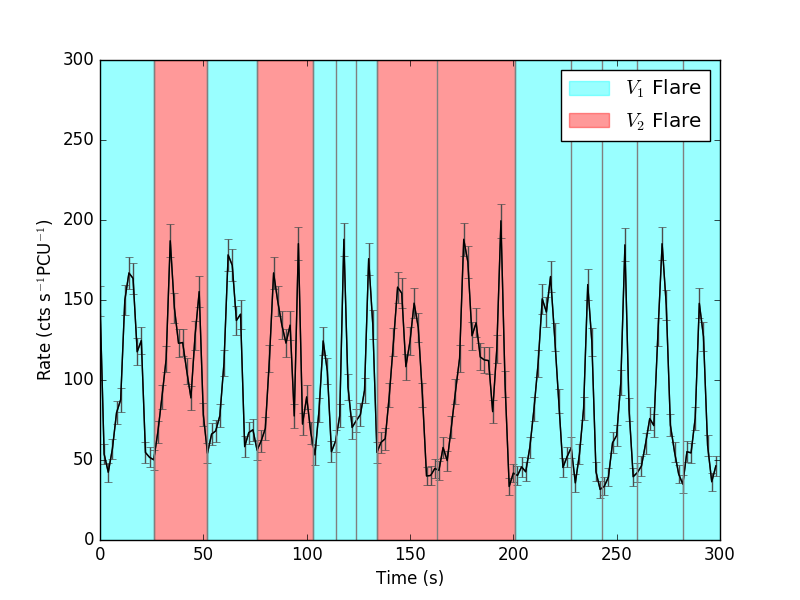
\includegraphics[width=\columnwidth, trim = 0mm 0mm 0mm 0mm]{images/KBurstTypes.png}
    \captionsetup{singlelinecheck=off}
    \caption[A portion of the lightcurve of observation 96420-01-06-03 showing Type $V_1$ flares and Type $V_2$ flares.]{A portion of the lightcurve of observation 96420-01-06-03, orbit 0, showing Type $V_1$ flares (highlighted in cyan) and Type $V_2$ flares (highlighted in red).}
   \label{fig:id_flares_V}
\end{figure}

\begin{figure}
    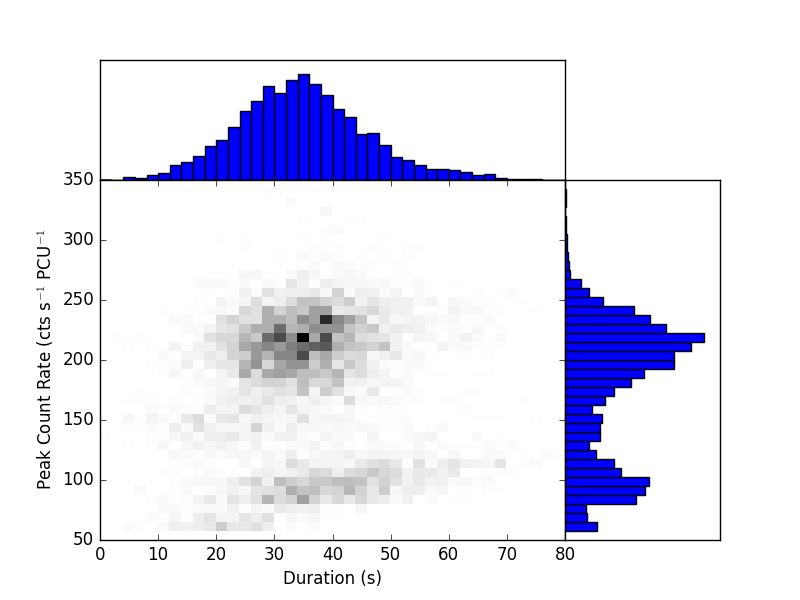
\includegraphics[width=\columnwidth, trim = 0mm 0mm 0mm 0mm]{images/KBurst.png}
    \captionsetup{singlelinecheck=off}
    \caption[Every flare in all observations identified as Class V, plotted in a two-dimensional histogram of flare peak count rate against flare duration to show the two-population nature of these events.]{Every flare in all observations identified as Class V, plotted in a two-dimensional histogram of flare peak count rate against flare duration to show the two-population nature of these events.}
   \label{fig:two_popV}
\end{figure}

\begin{figure}
    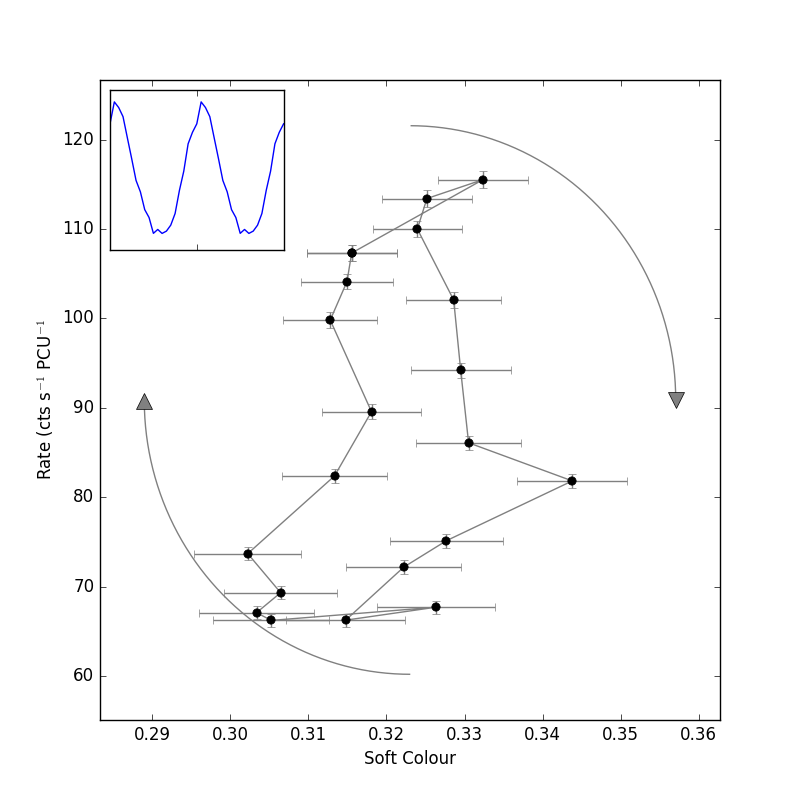
\includegraphics[width=\columnwidth, trim = 0mm 0mm 0mm 0mm]{images/Kloop.png}\\
    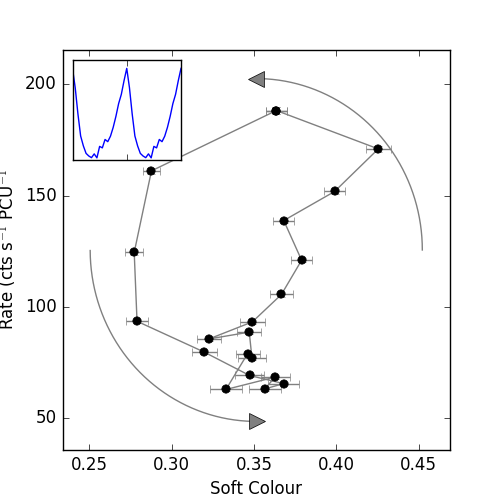
\includegraphics[width=0.5\columnwidth, trim = 0mm 0mm 0mm 0mm]{images/Kloop2.png}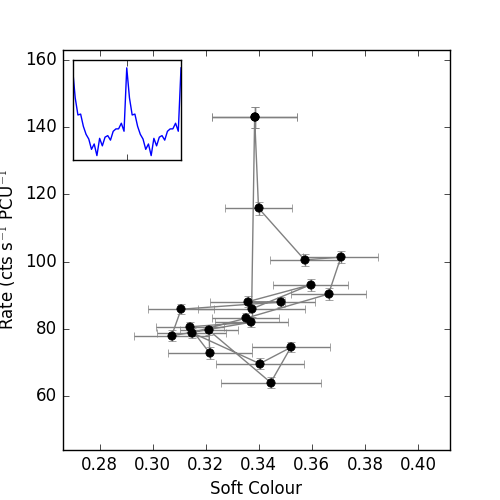
\includegraphics[width=0.5\columnwidth, trim = 0mm 0mm 0mm 0mm]{images/Kloop3.png}
    \captionsetup{singlelinecheck=off}
    \caption[The hardness-intensity diagram of a type $V_1$ flaring period in Class V observation 96420-01-07-00 showing a clockwise loop.]{\textit{Top}: The hardness-intensity diagram (HID$_1$) of a type $V_1$ flaring period in Class V observation 96420-01-07-00, orbit 0 showing a clockwise loop.  The data have been folded over a variable period found with the algorithm described in Section \ref{sec:Flares}.  Inset is the folded lightcurve of the same data. \textit{Bottom Left}: The hardness-intensity diagram of Class V observation 96420-01-25-05 orbit 0, an example of an anticlockwise loop.  \textit{Bottom Right}: The hardness-intensity diagram of Class V observation 96420-01-25-06 orbit 0, in which I was unable to ascertain the presence of a loop.}
   \label{fig:LoopV}
\end{figure}

\subsubsection{Class VI -- Figure \ref{fig:Lmulti}}

\begin{figure}
    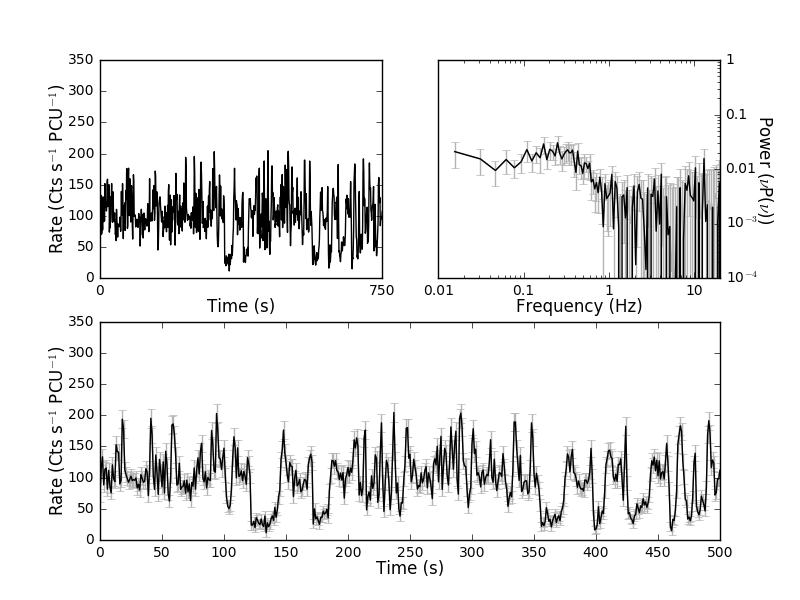
\includegraphics[width=0.8\columnwidth, trim = 0.6cm 0 3.9cm 0]{images/Lmulti.png}
    \captionsetup{singlelinecheck=off}
    \caption[Characteristic lightcurves and a power spectrum of Type VI variability.]{Plots of the Class VI observation 96420-01-09-00, orbit 0.  \textit{Top-left}: 750\,s lightcurve binned on 2 seconds to show lightcurve evolution.  \textit{Top-right}: Fourier Power Density Spectrum.  \textit{Bottom}: Lightcurve binned on 1 second.}
   \label{fig:Lmulti}
\end{figure}

\par The lightcurves of observations of this class show large dips in count rate; this can be seen in Figure \ref{fig:Lmulti} at, for example, $t\approx125$--$150$\,s .  These dips vary widely in duration, from $\sim5$ to $\sim50$ seconds, and the count rate in both $L_A$ and $L_B$ fall to a level consistent with background.  The dips' rise and fall times are fast, both lasting no longer than a second.  They do not appear to occur with any regular periodicity.
\par Aside from the dips, Class VI observations show other structures in their lightcurves.  Large fluctuations in count rate, by factors of $\lesssim3$, occur on timescales of $\sim1\mbox{--}5$ s; no periodicity in these oscillations could be found.  This behaviour is reflected in the PDS, which shows high-amplitude broad band noise below $\sim0.5$\,Hz with RMS-normalized power \citep{Belloni_RMSNorm} of up to $\sim1.1 $\,Hz$^{-1}$.  As can be seen in Figure \ref{fig:Lmulti}, this feature takes the form of a broad shoulder of noise which shows a either weak peak or no clear peak at all.  The $\sim5$\,Hz QPO seen in the PDS of other classes is not present in Class VI observations.
\par I attempted to fold all individual Class VI lightcurves, ignoring the sections of data corresponding to the large count rate dips described above.  In general, folding lightcurves belonging to this class is difficult; many orbits showed low-amplitude oscillations which were difficult to fold using my flare-finding algorithm (see Section \ref{sec:Flares}), while many others only showed oscillatory behaviour for a small number of periods between each pair of dips.  As such, I only succesfully folded 23 of the 40 Class VI orbits.  Of these, 19 showed clockwise loops in the HID$_1$ (top panel, Figure \ref{fig:LoopVI}), 3 showed anticlockwise loops (bottom-left panel, Figure \ref{fig:LoopVI}).  In the remaining 1 observation, the data did not allow us to ascertain the presence of loops (bottom-right panel, Figure \ref{fig:LoopVI}).
\par Like in Class VI, I note that the clockwise loops in Class VI appear more complex than clockwise loops.  Again, the clockwise loop shown in Figure \ref{fig:LoopVI} appears to have a 2-lobe structure; this is repeated in all clockwise loops found in this class.

\begin{figure}
    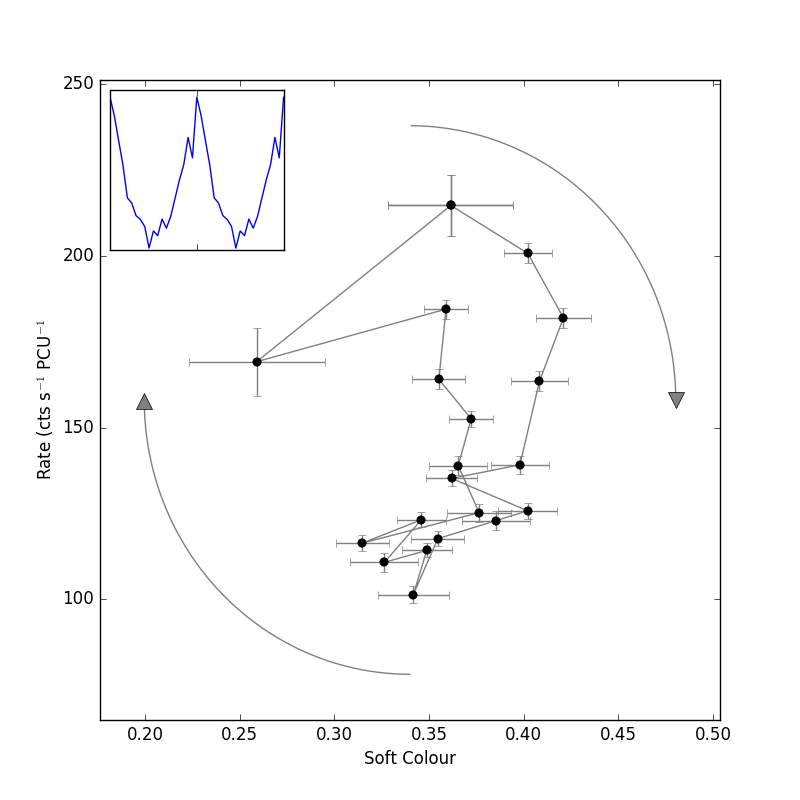
\includegraphics[width=\columnwidth, trim = 0mm 0mm 0mm 0mm]{images/Lloop2.png}\\
    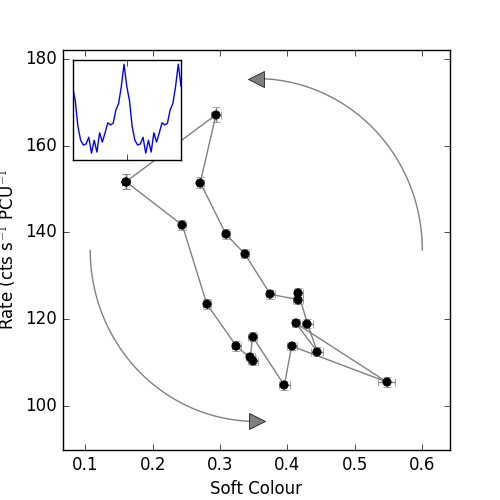
\includegraphics[width=0.5\columnwidth, trim = 0mm 0mm 0mm 0mm]{images/Lloop.png}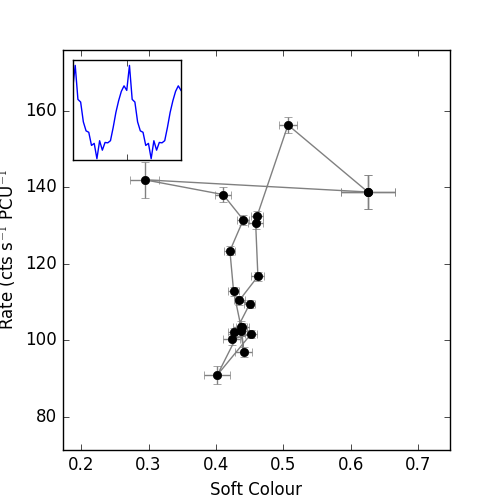
\includegraphics[width=0.5\columnwidth, trim = 0mm 0mm 0mm 0mm]{images/Lloop4.png}
    \captionsetup{singlelinecheck=off}
    \caption[The hardness-intensity diagram of the Class VI observation 96420-01-30-03, showing a clockwise loop.]{\textit{Top}: The hardness-intensity diagram (HID$_1$) of the Class VI observation 96420-01-30-03, orbit 0 showing a clockwise loop.  The data have been folded over a variable period found with the algorithm described in Section \ref{sec:Flares}.  Inset is the folded lightcurve of the same data. \textit{Bottom Left}: The hardness-intensity diagram of Class VI observation 96420-01-30-04 orbit 0, an example of an anticlockwise loop.  \textit{Bottom Right}: The hardness-intensity diagram of Class VI observation 96420-01-09-03 orbit 0, in which I was unable to ascertain the presence of a loop.}
   \label{fig:LoopVI}
\end{figure}

\subsubsection{Class VII -- Figure \ref{fig:Nmulti}}

\begin{figure}
    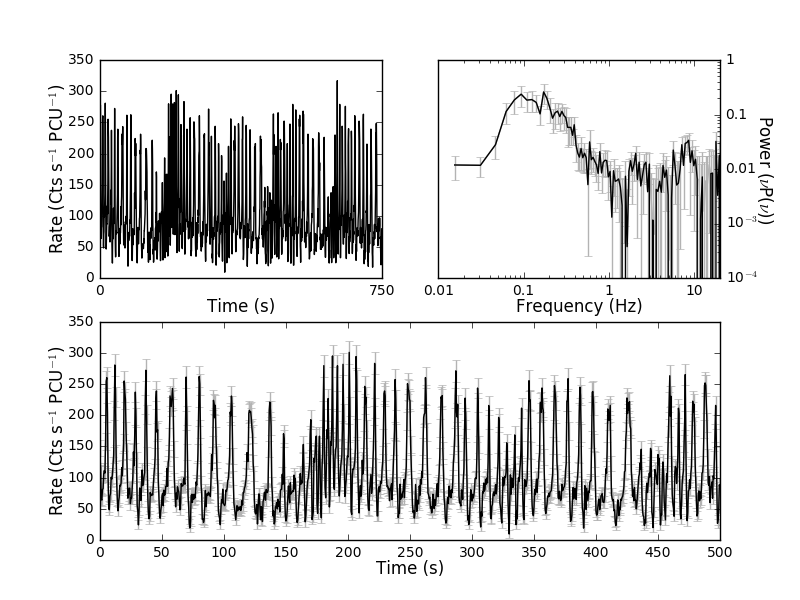
\includegraphics[width=0.8\columnwidth, trim = 0.6cm 0 3.9cm 0]{images/Nmulti.png}
    \captionsetup{singlelinecheck=off}
    \caption[Characteristic lightcurves and a power spectrum of Type VII variability.]{Plots of the Class VII observation 96420-01-18-05, orbit 0.  \textit{Top-left}: 750\,s lightcurve binned on 2 seconds to show lightcurve evolution.  \textit{Top-right}: Fourier Power Density Spectrum.  \textit{Bottom}: Lightcurve binned on 0.5 seconds.}
   \label{fig:Nmulti}
\end{figure}

\par Class VII shows high-amplitude flaring behaviour with a peak-to-peak recurrence time of $6$--$12$\,s.  In Figure \ref{fig:spect} I show a dynamical Lomb-Scargle spectrogram of a Class VII observation, showing that the fast flaring behaviour has a frequency which moves substantially over time.  This in turn accounts for the large spread in the value of the flare peak-to-peak recurrence time.
\par In Figure \ref{fig:spect} I show that the peak frequency of the QPO also varies in a structured way.  I also suggest that the variabilitity of the frequency is itself a QPO with a period of $\sim150$\,s.
\par At higher frequencies, the PDS shows a weak QPOs centred at $\sim8$\,Hz, with a $q$-values of $\sim2$.
\par I used my flare-finding algorithm (see Section \ref{sec:Flares}) to perform variable-frequency folding of Class VII orbits.  I find clockwise loops in 9 out of 11 Class VII orbits.  In the remaining two observations, the oscillations were extremely fast.  As a result, the errors in the HID$_1$ of these too observations were too large to succesfully select peaks, and I am unable to confirm or reject the presence of loops.

\begin{figure}
    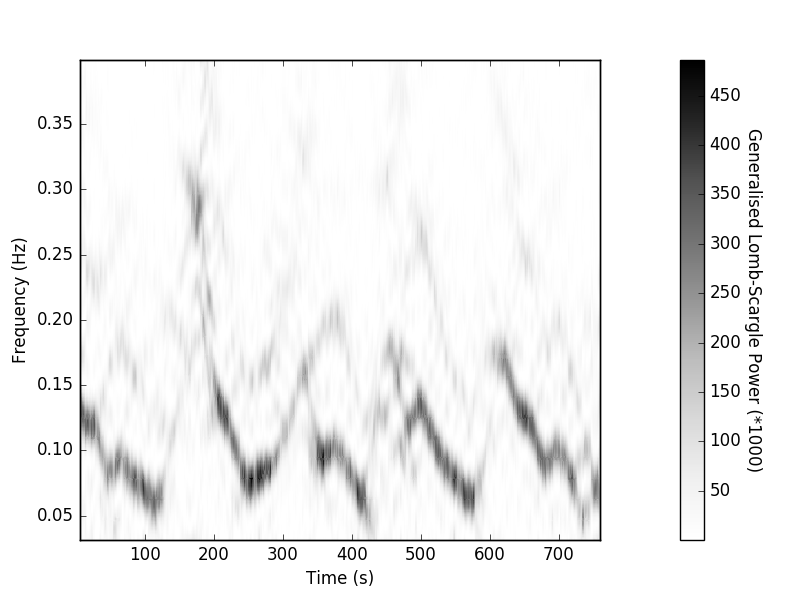
\includegraphics[width=0.8\columnwidth, trim = 0.6cm 0 3.9cm 0]{images/N_sgram.png}
    \captionsetup{singlelinecheck=off}
    \caption[A sliding window Lomb-Scargle spectrogram of Class VII observation 96420-01-18-05.]{A sliding window Lomb-Scargle spectrogram of Class VII observation 96420-01-18-05, showing power density spectra from an overlapping 32\,s window moved 1\,s at a time.  The peak frequency of this low frequency QPO itself appears to oscillate with a frequency of $\sim5$mHz.}
   \label{fig:spect}
\end{figure}

\subsubsection{Class VIII -- Figure \ref{fig:Omulti}}

\begin{figure}
    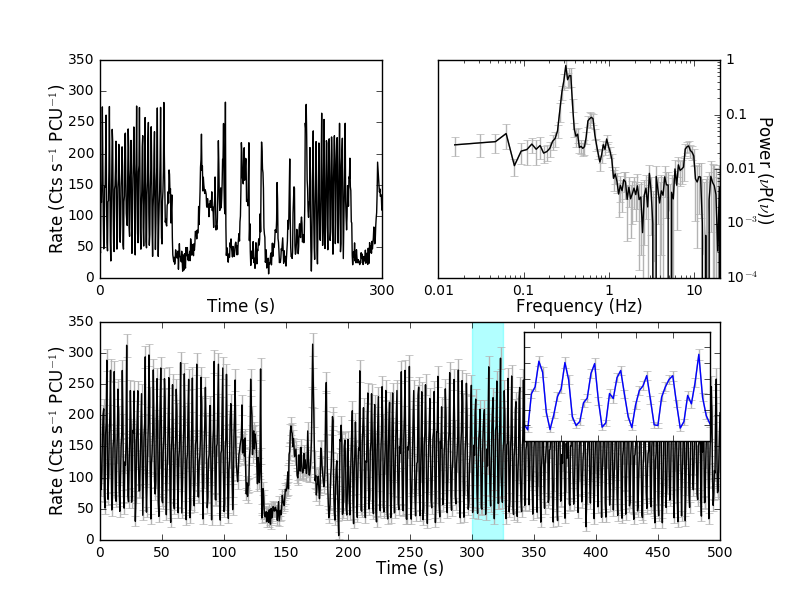
\includegraphics[width=0.8\columnwidth, trim = 0.6cm 0 3.9cm 0]{images/Omulti.png}
    \captionsetup{singlelinecheck=off}
    \caption[Characteristic lightcurves and a power spectrum of Type VIII variability.]{Plots of the Class VIII observation 96420-01-19-03, orbit 0.  \textit{Top-left}: 300\,s lightcurve binned on 2 seconds to show lightcurve evolution.  \textit{Top-right}: Fourier Power Density Spectrum.  \textit{Bottom}: Lightcurve binned on 0.5 seconds.  Inset is a zoom of the 25\,s portion of the lightcurve highlighted in cyan, to show the second-scale structure in the lightcurve.}
   \label{fig:Omulti}
\end{figure}

\par The lightcurve of this variability class shows the dipping behaviour seen in Class VI, as can be seen in Figure \ref{fig:Omulti} at $t\approx125$--$150$\,s.  The dips are less frequent than in Class VI.  The behaviour outside of the dips is dominated by highly structured high-amplitude oscillations consisting of flares with a peak to peak separation of $3.4\pm1.0$\,s.  The PDS shows this behaviour as a very significant ($q$-value > 20) QPO; two harmonics of this QPO are also visible.  The PDS also shows a strong ($q$-value = 4.7) QPO at $\sim9$\,Hz.
\par I attempted to fold Class VIII lightcurves, ignoring the portions of data corresponding to dips, using my flare-finding algorithm.  The high frequency of the dominant oscillation in Class VIII resulted in large errors in the peak times of individual flares, which translated to large errors in all HID$_1$s; however, I was able to ascertain the presence in loops in 8 out of 16 orbits.  All 8 of these loops are clockwise.

\subsubsection{Class IX -- Figure \ref{fig:Qmulti}}
\label{sec:ClassIX}
\begin{figure}
    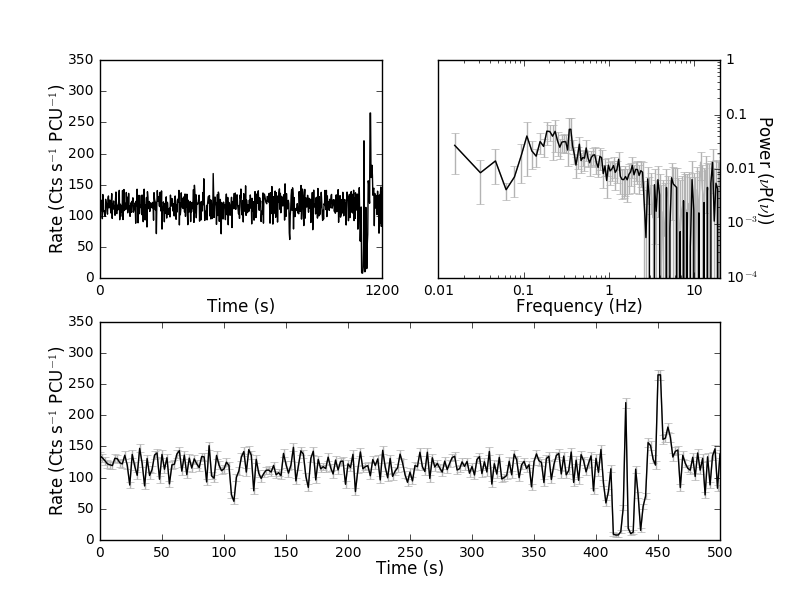
\includegraphics[width=0.8\columnwidth, trim = 0.6cm 0 3.9cm 0]{images/Qmulti.png}
    \captionsetup{singlelinecheck=off}
    \caption[Characteristic lightcurves and a power spectrum of Type IX variability.]{Plots of the Class IX observation 96420-01-35-02, orbit 1.  \textit{Top-left}: 1200\,s lightcurve binned on 2 seconds to show lightcurve evolution.  \textit{Top-right}: Fourier Power Density Spectrum.  \textit{Bottom}: Lightcurve binned on 2 seconds.}
   \label{fig:Qmulti}
\end{figure}

\par The 1\,s lightcurve of a Class IX observation is superficially similar to the lightcurve of a Class I observation, with little obvious structured variability at timescales larger than 2 s; however, large count rate dips like those seen in Classes VI and VIII (e.g. the feature at $t\approx410$\,s in the lightcurve of Figure \ref{fig:Qmulti}) are very occasionally observed.  These dips may in turn be coupled to short second-scale flares in which count rate briefly increases by a factor of 2--3.
\par Outside of these dips and flares, the lightcurve of a Class IX observation is indistinguishable from the lightcurve of a Class I or Class II observation.  However, in Figure \ref{fig:IIIisHarder}, I show that Class IX occupies a very different part of the global $H_{A2}$/$H_{A1}$ colour-colour diagram.  Class IX observations show a significantly larger $H_{A2}$ than Class I and II observations, but a significantly lower $H_{A1}$.
\par The PDS reveals significant broad band noise peaked at $\sim$0.3 Hz, and the $\sim5$\,Hz QPO seen in other classes is absent.  \citet{Altamirano_HFQPO} discovered high frequency ($\sim66$\,Hz) QPOs in observations corresponding to this variability class.

\subsection{Swift}

\par Observations with \textit{Swift} took place throughout the 2011-2013 outburst of IGR J17091-3624.  Between MJDs 55622 and 55880, 17 \textit{Swift/XRT} were at least partly simultaneous with an \rxte\ observation, corresponding to at least one observation of all 9 classes.  In each case, the \textit{Swift} and \rxte\ lightcurves were similar.  The remainder of the \textit{Swift/XRT} observations during this time were also consistent with belonging to one of my nine classes.  Given that the \rxte\ data have higher count rate and time resolution, I do not further discuss the \textit{Swift} observations taken before MJD 55880.  A more detailed comparison of \rxte\ and \textit{Swift} data is beyond the scope of this thesis.
\par Between MJD 55952 and 56445, \textit{Swift} observations showed IGR J17091-3624 decreasing in flux.  For all observations longer than 500 s, I rebinned the lightcurves to 10\,s and calculated the RMS.  I find the lower and upper quartiles of the fractional RMS in these measurements to be 18.3\% and 21.7\% respectively.  \textit{INTEGRAL} observations taken as part of a scan programme of the Galactic Plane \citep{Fiocchi_PlaneScan} and reported by \citet{Drave_Return} suggest that IGR J17091-3624 returned to the hard state between MJDs 55952 and 55989.  Therefore these observations sample IGR J17091-3624 the hard state.

\subsection{INTEGRAL}

\par The results of the \textit{INTEGRAL}/IBIS analysis are presented in Table \ref{tab:IBIS_results}. \textsf{C.B.} finds clear detections of IGR J17091-3624 in all energy bands during the hardest period (MJD 55575--55625) of the 2011--2013 outburst. Conversion from detected counts to flux was achieved using an \textit{INTEGRAL}/IBIS observation of the Crab taken between MJD 57305.334 and 57305.894. Conversion from Crab units to standard flux units was obtained by conversion factors listed in \citet{Bird_Survey} and \citet{Bazzano_Survey}.

\begin{table*}
\begin{tabular}{cccccc}
\hline
\hline
Energy 		& Intensity 		& Significance 	& Exposure 	& Flux 				& Flux					\\
(keV)		& (cts/s)			& $\sigma$		& (ks)		& (mCrab) 			& (10$^{-10}$ergs~s$^{-1}$~cm$^{-2}$) 	\\
\hline
20--40		& 12.39$\pm$0.05	& 247			& 115		& 93.5$\pm$0.38		& 7.08$\pm$0.03			\\
40--100		& 7.06$\pm$0.05		& 157			& 163		& 83.5$\pm$0.60		& 7.87$\pm$0.06			\\
100--150	& 1.05$\pm$0.03		& 40			& 173		& 66.9$\pm$1.91		& 2.14$\pm$0.06			\\
150--300	& 0.23$\pm$0.03		& 7.6			& 179		& 46.6$\pm$5.96		& 2.24$\pm$0.29			\\	
\hline
\hline
\end{tabular}
\caption[Results from the IBIS/ISGRI analysis of the 2011--2013 Outburst of IGR J17091.]{Results from the IBIS/ISGRI analysis of the 2011--2013 Outburst of IGR J17091. The 20--40\,keV flux is given in units of mCrab and (10$^{-11}$\ergf ). Conversion between counts and mCrab was obtained using an observation of the Crab taken during Revolution 1597 between MJD 57305.334 and 57305.894 and the conversion factors of \citet{Bird_Survey} and \citet{Bazzano_Survey}.}
\label{tab:IBIS_results}
\end{table*}

\par Comparing these results with those of \citet{Bazzano_Survey}, we see that IGR J17091 is detected for the first time above 150\,keV with a detection significance of 7.6\,$\sigma$, corresponding to a flux of $2.24\pm0.29\times10^{-10}$\ergf\ (Figure \ref{fig:sigmap}).

\begin{figure}
    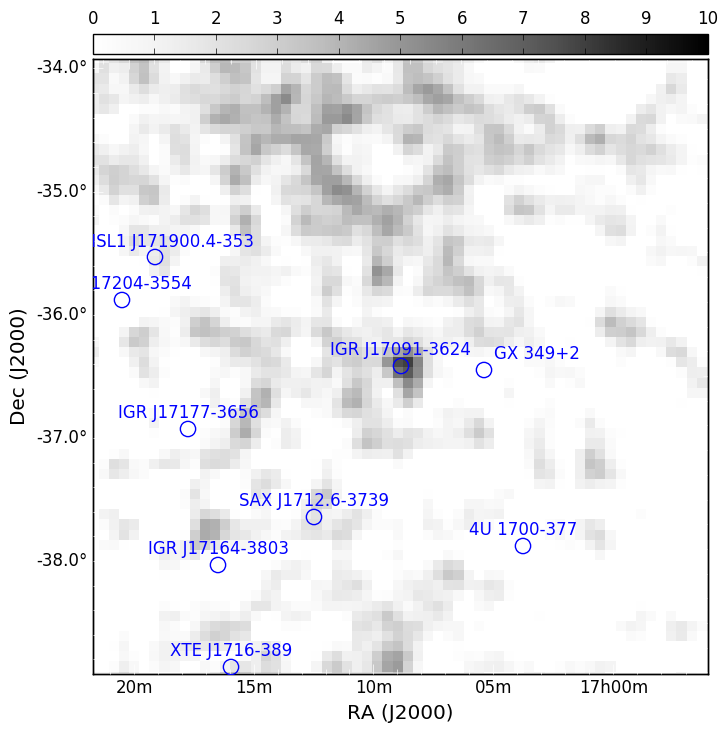
\includegraphics[width=0.7\columnwidth, trim = 0.6cm 0 3.9cm 0]{images/sigmap.png}
    \captionsetup{singlelinecheck=off}
    \caption[\textit{INTEGRAL}/ISGRI 150--300\,keV significance map of a $2^\circ$ region centred on the position of IGR J17091-3624.]{\textit{INTEGRAL}/ISGRI 150--300\,keV significance map of a $2^\circ$ region centred on the position of IGR J17091-3624, showing the first significant detection of this source above 150\,keV.  The detection significance is 7.6 $\sigma$.}
   \label{fig:sigmap}
\end{figure}

\subsection{Chandra}

\par In Figure \ref{fig:Cha_lc}, I present lightcurves from the three \textit{Chandra} observations considered in this chapter (see also Table \ref{tab:Chandra} for details of these observations).

\begin{figure}
    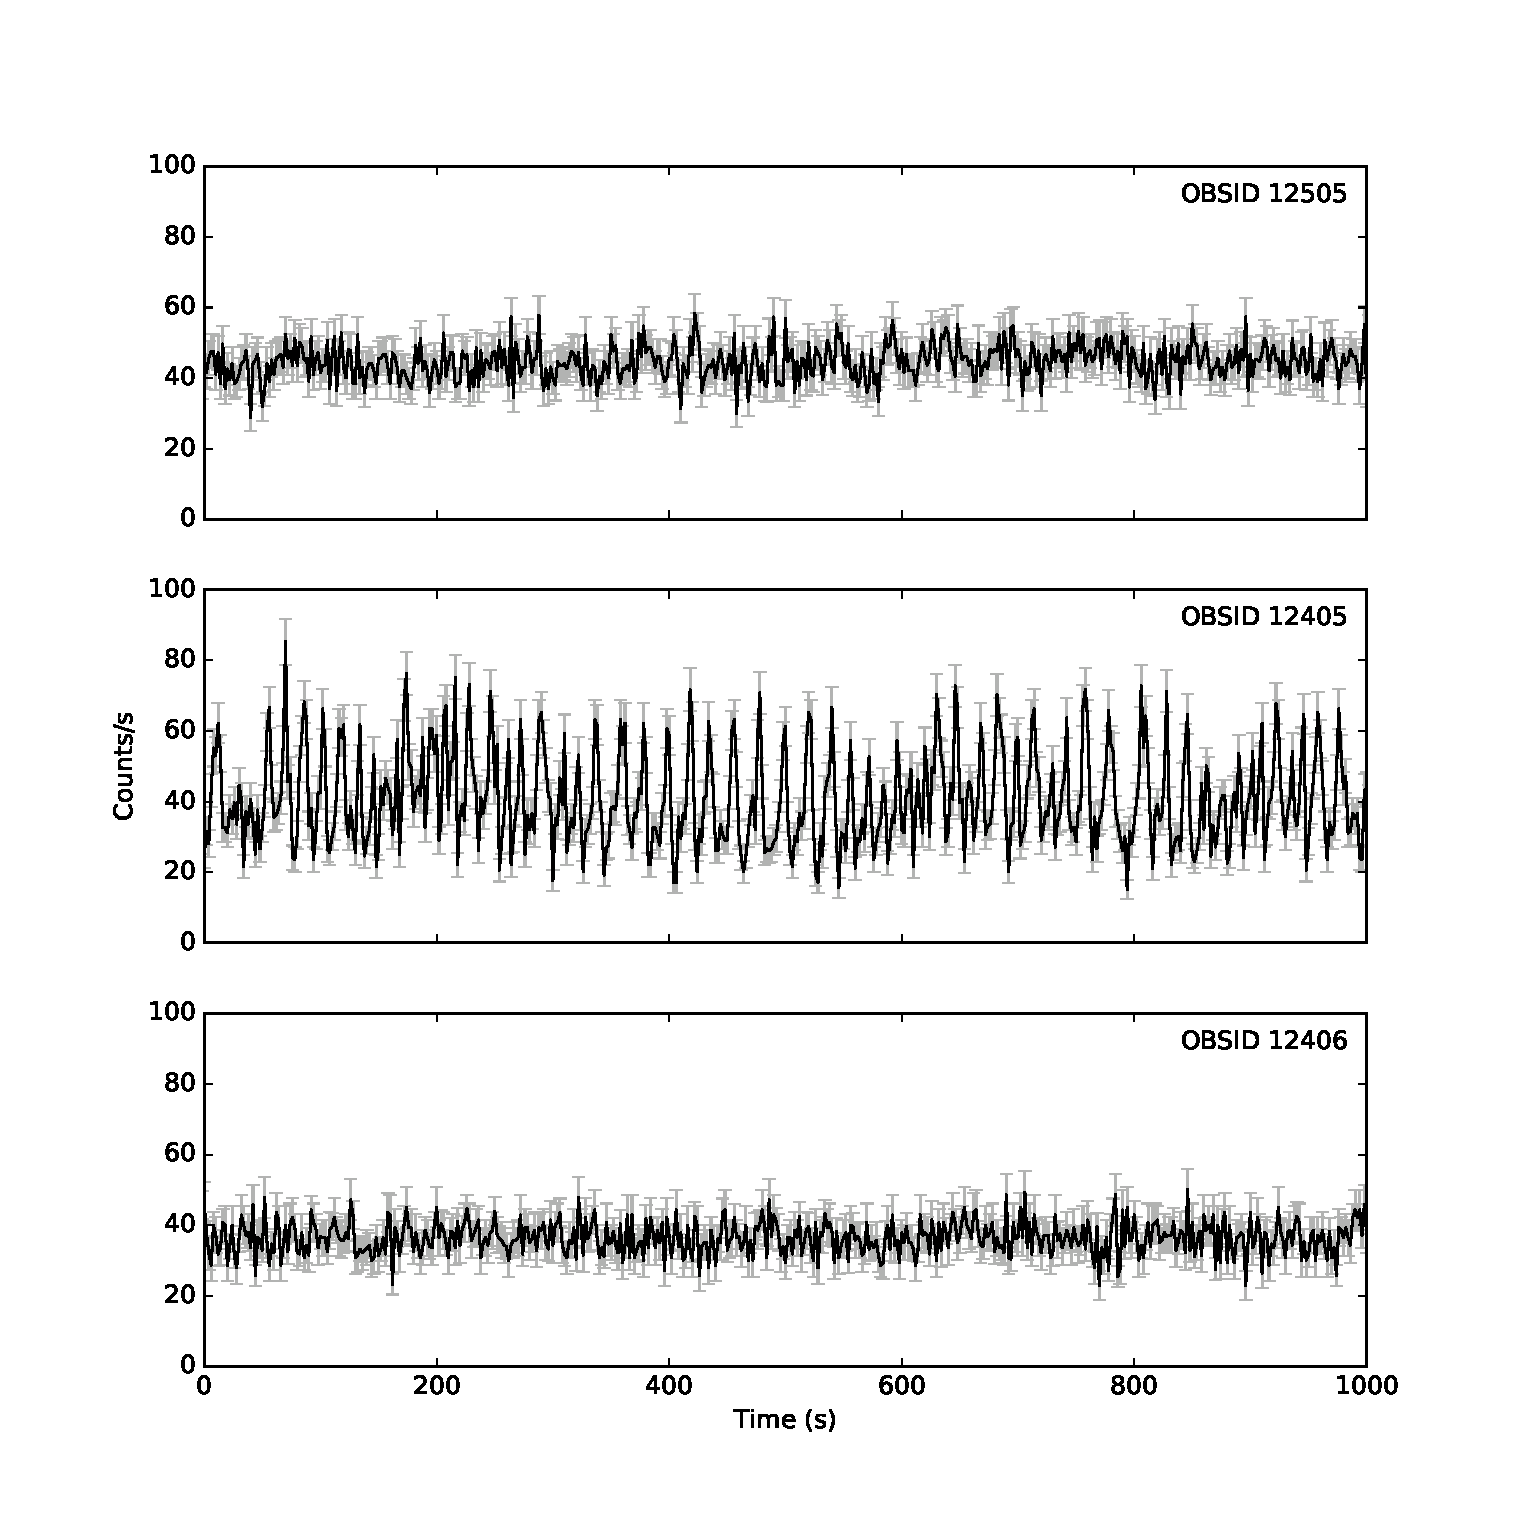
\includegraphics[width=0.8\columnwidth, trim = 0.6cm 0 3.9cm 0]{images/Chandra.eps}
    \captionsetup{singlelinecheck=off}
    \caption[\textit{Chandra} lightcurves showing examples of Class I, VII and IX variability.]{1 ks segments of lightcurves taken from \textit{Chandra} observations 12505, 12405 and 12406, showing Class I, Class VII and Class IX variability respectively.  The lightcurve presented for observation 12505 is for the energy range 0.06-10\,keV, while the other two lightcurves are for the energy range 0.5-10\,keV.  All three lightcurves are binned to 0.5\,s.}
   \label{fig:Cha_lc}
\end{figure}

\par Observation 12505 was performed within 24 hours of \rxte\ observation 96420-01-02-01, which showed Class I variability.  No structured variability is seen in the lightcurve of ObsID 12505 (Figure \ref{fig:Cha_lc}, upper panel), which is consistent with Class I.  Note that I consider the energy range 0.06-10\,keV for this observation but 0.5-10\,keV for observations 12405 and 12406.
\par Observation 12405 was performed within 24 hours of \rxte\ observation 96420-01-23-03, which showed Class V variability.  The two observations were not simultaneous; ObsID 12405 began $\sim8.4$ ks after ObsID 96420-01-2303 finished.  The lightcurve of \textit{Chandra} ObsID 12405 (shown in Figure \ref{fig:Cha_lc}, middle panel) shows a mean count rate of 41\,cts\,s$^{-1}$.  The lightcurve shows fast flaring behaviour (with a recurrence time on the order of 10s of seconds) in which the frequency changes widely on timescales of $\sim1000$\,s.  This observation strongly resembles a Class VII lightcurve, but with its characteristic timescales increased by a factor of $\sim4$.  This leads to the possibility that the low number of Class VII \rxte\ observations I identify is due to a selection effect; we would not have been able to see this observation's long-term Class VII-like behaviour if the observation had been shorter than $\sim2$ ks.
\par Observation 12406 was performed within 24 hours of \rxte\ observation 96420-01-32-06, which showed Class IX variability.  The lightcurve presented for \textit{Chandra} ObsID 12406 shows a mean count rate (36 cts s$^{-1}$), which is consistent with IGR J17091 being harder in this observation than in Observation 12505.  This, combined with the lack of variability seen in its lightcurve, suggests that Observation 12505 is consistent with Class IX.

\subsection{XMM-Newton}

\par In Figure \ref{fig:XMM} I show lightcurves from two \textit{XMM-Newton} observations.  The lightcurve of \textit{XMM-Newton} observation 0677980201, shown in the upper panel of Figure \ref{fig:XMM}, shows the regular flares characteristic of Class IV variability.  A simultaneous \rxte\ observation (ObsID 96420-01-05-000) also showed Class IV variability.

\begin{figure}
    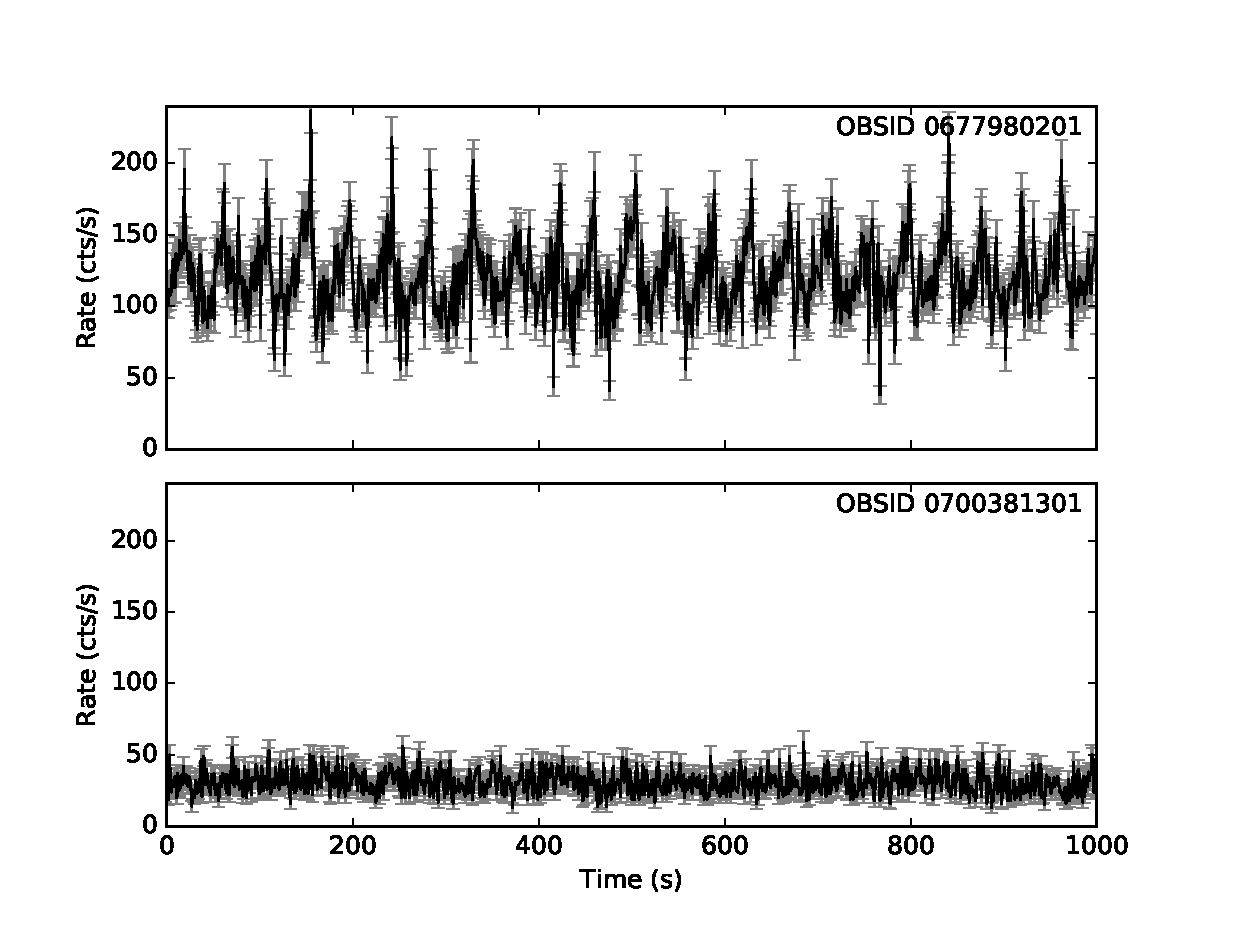
\includegraphics[width=0.8\columnwidth, trim = 0.6cm 0 3.9cm 0]{images/xmmlc.eps}
    \captionsetup{singlelinecheck=off}
    \caption[\textit{XMM-Newton} lightcurves showing an example of Class IV variability and the hard state.]{Lightcurves of \textit{XMM-Newton} observations 0677980201 and 0700381301, showing Class IV variability and the hard state respectively.  Both lightcurves binned to 2\,s.  Data for observation 0677980201 is taken from \textit{EPIC-MOS2} and data for observation 0700381301 is taken from \textit{EPIC-pn}.}
   \label{fig:XMM}
\end{figure}

\par \textit{XMM-Newton} observation 070038130, shown in the lower panel of Figure \ref{fig:XMM}, was made after the end of \rxte\ observations IGR J17091-3624.  As such it cannot be compared with contemporaneous \rxte\ data.  The 5\,s binned lightcurve shows no apparent variability, but a Fourier PDS of the observation (shown in Figure \ref{fig:xmmqpo}) reveals a QPO centred at around $\sim0.15$\,Hz and a broad band noise component at lower frequencies.  \citet{Drave_Return} reported that IGR J17091 transited to the hard state in February 2012, seven months before this observation was taken.  As such, I find that observation 0677980201 samples the hard state in IGR J17091 and is thus beyond the scope of my set of variability classes.

\begin{figure}
    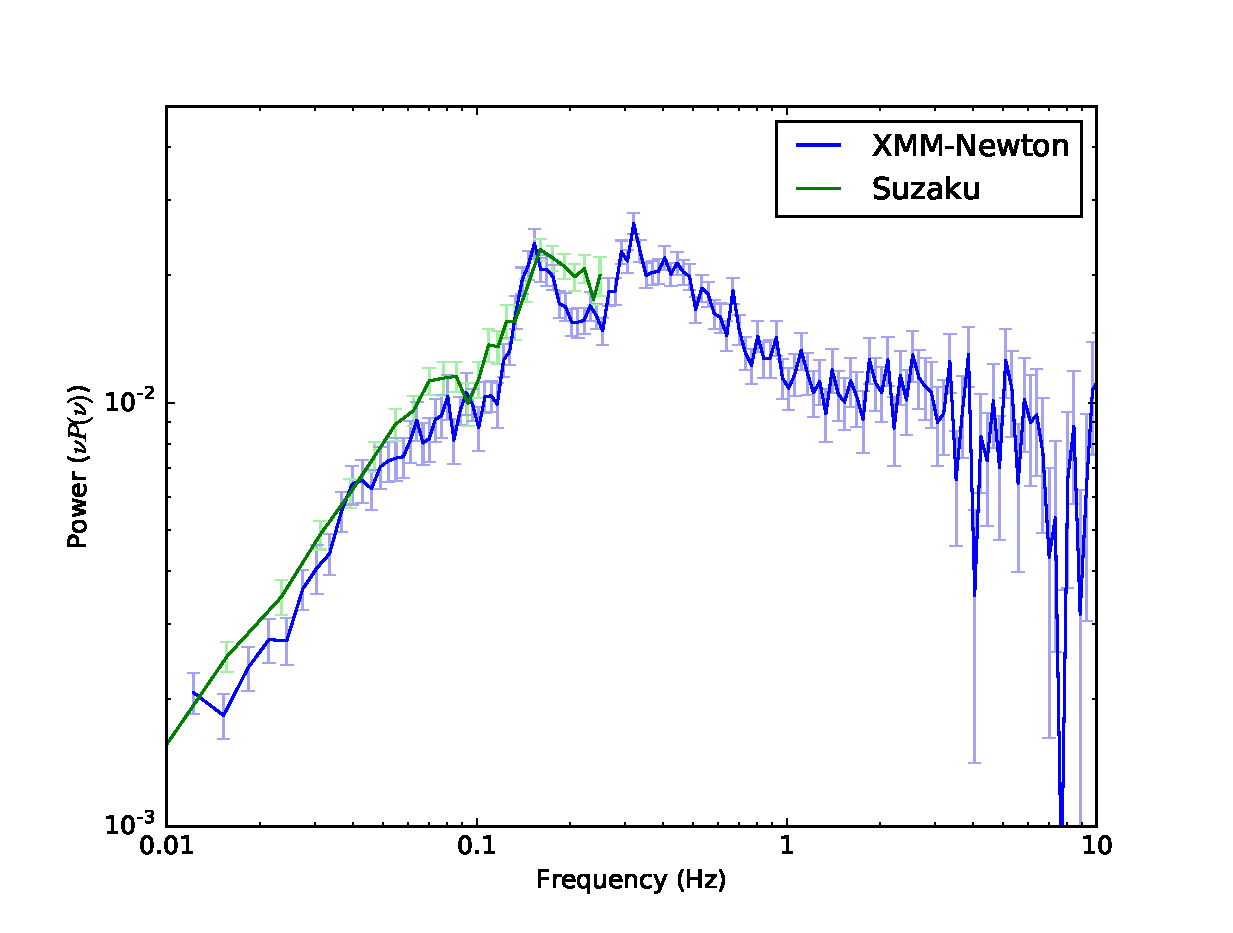
\includegraphics[width=0.9\columnwidth, trim = 0cm 0cm 0.5cm 1.0cm, clip]{images/multipower.eps}
    \captionsetup{singlelinecheck=off}
    \caption[$\nu P(\nu)$-normalised co-added power density spectra of \textit{XMM-Newton} observation 0700381301 and \textit{Suzaku} observation 407037010.]{$\nu P(\nu)$-normalised co-added power density spectra of \textit{XMM-Newton} observation 0700381301 and \textit{Suzaku} observation 407037010.  Both observations were taken simultaneously on September 29 2012 (MJD 56199).  I sample observation 0700381301 up to a frequency of 10\,Hz, while the 2\,s time resolution of observation 407037010 results in a Nyquist frequency of 0.25\,Hz.}
   \label{fig:xmmqpo}
\end{figure}

\subsection{\textit{Suzaku}}

\par The two {\it Suzaku} observations of IGR J17091-3624 considered, ObsIDs 407037010 and 407037020, were performed during the 2nd and 3rd re-flares of the hard state phase of the 2011--2013 outburst.  ObsID 407037010 was taken simultaneously with \textit{XMM-Newton} observation 0700381301.  The XIS 0 count rates are 7.8 cts\,s$^{-1}$ and 2.5\,cts\,s$^{-1}$ respectively.
\par Neither lightcurve shows `heartbeats' or any other type of GRS 1915-like variability.  However, \textsf{K.Y.} and I find evidence of a low frequency QPO feature at $\sim$0.15 Hz in the ObsID 407037010; this QPO is also seen in \textit{XMM-Newton} observation 0700381301 (Figure \ref{fig:xmmqpo}).  The presence of a QPO below 1\,Hz and flat-topped power density spectrum confirm that IGR J17091 was in the hard state at this time.

\section{Discussion}

\par Using observations from \textit{XMM-Newton}, \rxte\ and \textit{Chandra}, I describe the complex variability seen in IGR J17091 as a set of nine variability `classes', labelled I to IX.  These classes are distinguished from each other by values of upper and lower quartile (i.e. 25\textsuperscript{th} and 75\textsuperscript{th} percentile) count rates, mean RMS, the presence of QPOs in Fourier PDS, the shape of flare and dip features in the lightcurve and the presence of loops in the 6--16/2--6 keV hardness-intensity diagram HID$_1$.  See Section \ref{sec:results} for a full description of these classes.
\par The classification of some observations is clearer than others.  Some orbits were too short to definitively quantify the behaviour of the source, whereas some other orbits contain a transition between two classes.  An example lightcurve showing a transition from Class III to Class IV is presented in Figure \ref{fig:HybridClasses}.

\begin{figure}
    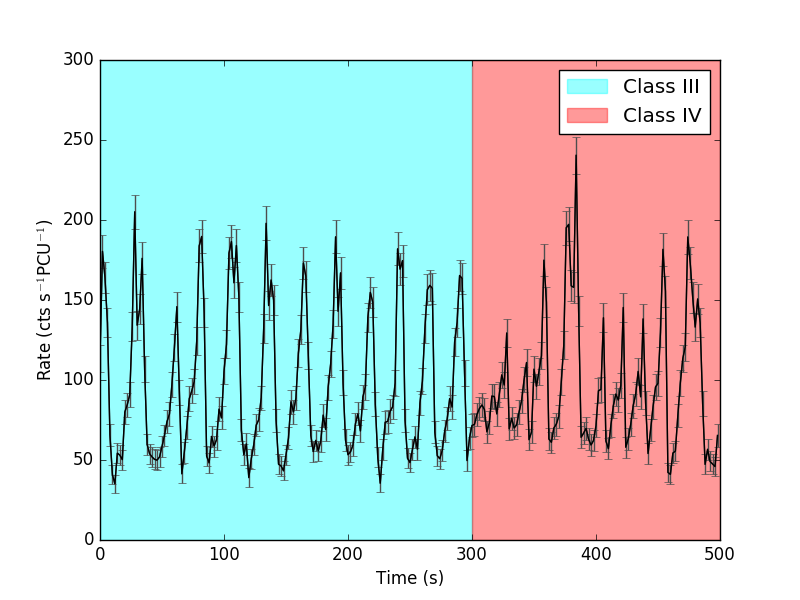
\includegraphics[width=\columnwidth, trim =0cm 0 0cm 0]{images/mixJandK.png}
    \captionsetup{singlelinecheck=off}
    \caption[A lightcurve of observation 96420-01-06-02, showing a transition in behaviour between Classes IV and V.]{A lightcurve of observation 96420-01-06-02, orbit 0, showing a transition in behaviour between Class III (in cyan, see Section \ref{sec:classIII}) and Class IV (in red, see Section \ref{sec:classIV}).}
   \label{fig:HybridClasses}
\end{figure}

\par My set of classes is analogous to, but not based upon, the set of variability classes defined by \citealt{Belloni_GRS_MI} to describe the behaviour of the similarly complex LMXB GRS 1915.  This ensures that my set of classes is not biased by an \textit{a priori} assumption that the two objects are similar.  However if we do assume that wide range of variability seen in these two objects are driven by the same physical processes, a direct comparison between the variability classes in the two systems can further our understanding of the physics that drive these exotic objects.
\par I also use all 2011-2013 IGR J17091-3624 data from \rxte , \textit{XMM-Newton}, \textit{Chandra}, \textit{Swift}, \textit{INTEGRAL} and \textit{Suzaku} to analyse the long-term evolution of the 2011--2013 outburst.  This in turn corresponds to all available X-ray data taken during this outburst.

\subsection{Variability Classes: IGR J17091 vs. GRS 1915}

\par As observations of IGR J17091 and GRS 1915 suffer from different values of interstellar absorption $N_H$\footnote{$N_H$, or the interstellar absorption, is a measure of the surface density of hydrogen atoms along a column between the object in question and the Earth.}, I cannot directly compare the absolute colours of these two objects.  However, I can compare the evolution of colour both over time and as a function of count rate.  I therefore use these parameters, along with power spectra and lightcurve morphology, when comparing GRS 1915 with IGR J17091.
\par For seven of my classes, I was able to assign the closest matching class described by \citealt{Belloni_GRS_MI} for GRS 1915 (see Table \ref{tab:class_assign}).  I am unable to find analogues to my classes VII and VIII in observations of GRS 1915, and I suggest that these classes are unique to IGR J17091.

\begin{table}
\centering
\caption[The nine variability classes of IGR J17091-3624, showing the name of the closest corresponding variability class in GRS 1915+105.]{The nine variability classes of IGR J17091-3624, showing the name of the closest corresponding variability class in GRS 1915+105.  The names of GRS 1915+105 classes are taken from \citet{Belloni_GRS_MI}, where more detailed descriptions can be found.  Eight additional classes of GRS 1915+105 have been described; I do not find analogies to these classes in IGR J17091-3624.}
\label{tab:class_assign}
\begin{tabular}{cc} % four columns, alignment for each
\hline
\hline
IGR J17091-3624 Class & GRS 1915+105 Class\\
\hline
I&$\chi$\\
II&$\phi$\\
III&$\nu$\\
IV&$\rho$\\
V&$\mu$\\
VI&$\lambda$\\
VII&\textit{None}\\
VIII&\textit{None}\\
IX&$\gamma$\\
\hline
\hline
\end{tabular}
\end{table}

\par Below, I evaluate my mapping between GRS 1915 and IGR J17091 classes, and interpret the differences between each matched pair.

\subsubsection{Classes I and II -- Figures \ref{fig:Bmulti}, \ref{fig:Emulti}}

\label{sec:DisI}

\par Classes I and II both show low count rates and little structure in their lightcurves.  The two classes in GRS 1915 that also show this lightcurve behaviour are Class $\chi$\footnote{Note that, in GRS 1915+105, Class $\chi$ is further subdivided into four classes based on hard colour \citep{Belloni_GRS_MI,Pahari_Chi}.  As I cannot obtain hard colour for IGR J17091, I treat $\chi$ as a single variability class here.} and Class $\phi$.  \citealt{Belloni_GRS_MI} differentiate between Classes $\phi$ and $\chi$ based on the hard colour (corresponding to $C_2$), as Class $\chi$ has a significantly higher value for this colour than Class $\phi$.

\par Data from \rxte\  indicates that the transition from the hard state to the soft intermediate state between MJDs 55612 and 55615 \citep{Drave_Return}.  This was confirmed by a radio spectrum taken on MJD 55623 which was consistent with an observation of discrete ejecta \citep{Rodriguez_D}.  This observation of discrete ejecta at the transition between the hard state and the intermediate state has been reported in other LMXBS (e.g. XTE J1550-564, \citealp{Rodriguez_XTE}), and has also been associated with transitions to the $\chi$ Class in GRS 1915 (\citealp{Rodriguez_Ejection}, see also review by \citealp{Fender_Jets}).

\par Using Fourier PDS, I conclude that Class I is analogous to Class $\chi$ in GRS 1915, while Class II is analogous to Class $\phi$.  In Class $\chi$ observations of GRS 1915, broad band noise between $\sim1-10$\,Hz and a QPO at around 5\,Hz are seen in the PDS.  I find that both of these are present in Class I observations of IGR J17091.  On the other hand, I find that Class $\phi$ observations of GRS 1915 do not show this broad band noise, and show either a weak ($q$-value $\lesssim 3$) QPO at $\sim5$\,Hz or no QPO at all.  I find that the weak QPO and lack of broad band noise are also seen in the PDS of Class II observations.

\subsubsection{Classes III and IV -- Figures \ref{fig:Gmulti}, \ref{fig:Jmulti}}

\par Classes III and IV both show highly regular flaring activity in their lightcurves, but they differ in terms of timescale and pulse profile.  As can be seen in lightcurves in Figure \ref{fig:Jmulti}, flares in Class IV occur every $\sim32$\,s and are nearly identical to each other in shape.  On the other hand, as can be seen in Figure \ref{fig:Gmulti}, flares in Class III occur every $\sim61$\,s and may or may not end in a much faster sharp peak which is never seen in Class IV.  In Figure \ref{fig:III_IV_burst} I show a two-dimensional histogram of flare peak count rate against flare duration, showing all flares in all observations classified as Class III or Class IV.  In this figure, I can see that flares tend to group in one of two regions in count rate-duration space; a region between $\sim90\mbox{--}110$ \spcu and $\sim35\mbox{--}55$\,s, corresponding to flares seen in Class III, and a region between $\sim150\mbox{--}250$ \spcu and $\sim20\mbox{--}55$\,s, corresponding to flares seen in Class IV.  From this plot, I conclude that the flares seen in Class III exist in a different population to the flares seen in Class IV.
\par The GRS 1915 classes that show behaviour most similar to these are $\rho$ and $\nu$; both produce similar structures in their lightcurve, but Class $\nu$ is differentiated from Class $\rho$ by the presence of a secondary count rate peak which occurs $\sim5$\,s after the primary \citep{Belloni_GRS_MI}.

\begin{figure}
    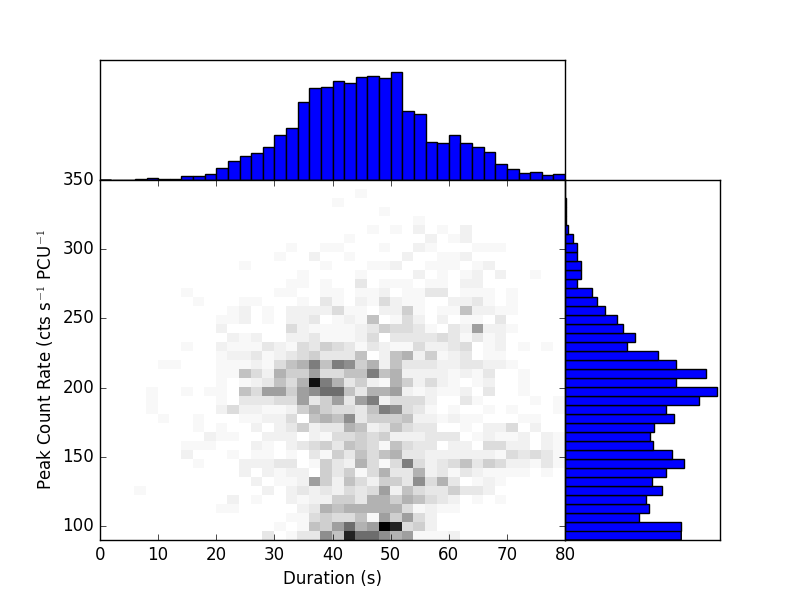
\includegraphics[width=\columnwidth, trim = 0mm 0mm 0mm 0mm]{images/GJBurst.png}
    \captionsetup{singlelinecheck=off}
    \caption[Every flare in all observations identified as Class III or Class IV, plotted in a two-dimensional histogram of flare peak count rate against flare duration to show the two-population nature of these events.]{Every flare in all observations identified as Class III or Class IV, plotted in a two-dimensional histogram of flare peak count rate against flare duration to show the two-population nature of these events.  Flares belonging to Class IV occupy the distribution at higher peak rate and lower duration, whereas flares belonging to Class III occupy the distribution at lower peak rate and higher duration.}
   \label{fig:III_IV_burst}
\end{figure}

\par The secondary peak is present in most Class III observations and some Class IV observations (Figure \ref{fig:III_IV_spike}), suggesting that both classes consist of a mix of $\rho$-like and $\nu$-like observations.  However, the poor statistics sometimes make the presence of this secondary peak difficult to detect.  As such, I do not use the presence or absence of this peak as a criterion when assigning classes.  Instead I choose to separate Classes III and IV based on the larger-scale structure in their lightcurves (see Section \ref{sec:classIV}).  Due to the aforementioned difference in burst populations between the two classes, I suggest that classes III and IV do represent two distinct classes rather than a single class with a period that drifts over time.  I suggest that Classes $\rho$ and $\nu$ in GRS 1915 could also be re-partitioned in this way.

\begin{figure}
    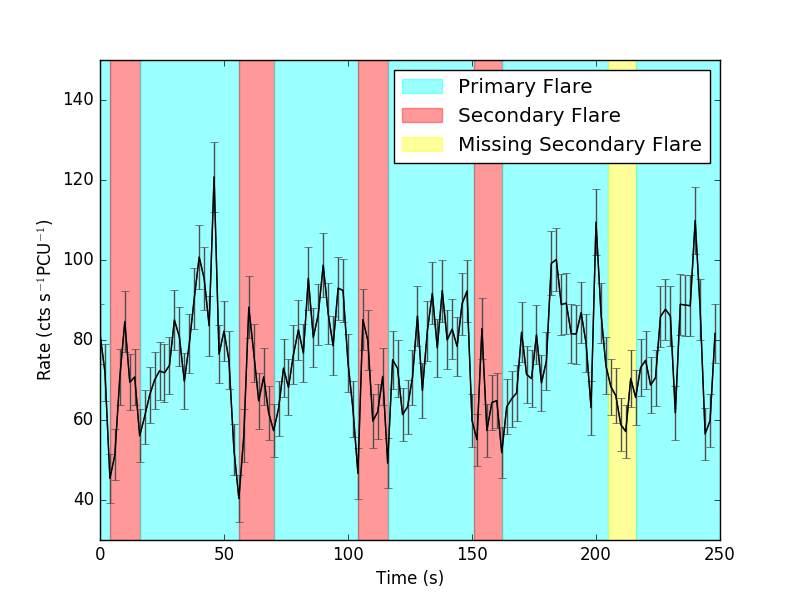
\includegraphics[width=\columnwidth, trim = 0mm 0mm 0mm 0mm]{images/classIIIsecpeak.png}
    \captionsetup{singlelinecheck=off}
    \caption[Lightcurve from Class III observation 96420-01-10-01 of IGR J17091-3624, with pairs of primary and secondary count rate spikes highlighted.]{Lightcurve from Class III observation 96420-01-10-01 of IGR J17091-3624, with pairs of primary and secondary count rate spikes highlighted in cyan and red respectively.  The yellow region highlights a primary count rate spike that did not produce a secondary.}
   \label{fig:III_IV_spike}
\end{figure}

\par However, HID$_1$ loops are found to generally execute in an anticlockwise direction in Classes III and IV (previously noted by e.g. \citealp{Altamirano_IGR_FH}); the opposite direction to the clockwise loops in Classes $\rho$ and $\nu$ reported by e.g. \citealp{Belloni_GRS_MI} and repeated by us using the same method I apply to data from IGR J17091-3624 (see Section \ref{sec:dex}).  This suggests that Classes III and IV could be generated by a different physical mechanism to Classes $\rho$ and $\nu$.  Alternatively, Classes III and IV could be generated by the same mechanism as $\rho$ and $\nu$ if some other unknown process was able to alter the spectral evolution of flares in these classes.

\subsubsection{Class V -- Figure \ref{fig:Kmulti}}

\par The lightcurve of a Class V observation appears similar to that of a Class $\mu$ observation of GRS 1915, as both are characterised by rapid $\rho$-like flares which occur less regularly than in Class $\rho$.  In addition to this, flares in Class $\mu$ fall into two clear populations, as do the flares in Class V.  However, significant differences exist between Class V and Class $\mu$.  Class $\mu$ observations are characterised by long ($\sim100$ s) excursions to plateaus of high count rate, a behaviour which is not seen in any Class V observation thus far.
\par I note that the HID$_1$ in Class V observations displays a loop in the clockwise direction; the opposite direction to the looping seen in Classes III and IV but the same direction seen in Class $\mu$.
\par Regarding the two-population nature of flares seen in this class (see Section \ref{sec:classV}), I suggest that V$_2$ flares may simply be two V$_1$ flares that occur close together in time, such that the second flare starts during the decay of the first flare.  This would result in an apparent two-peaked flare structure, as we see in type V$_2$ flares.  This interpretation also accounts for the bimodal distribution of flare duarations shown in the 2D histogram of Figure \ref{fig:two_popV}, as this could be caused by the misinterpretation of two-flare V$_2$ events as a single event.  This also accounts for the Gaussian distribution of peak flare intensities seen in Figure \ref{fig:two_popV}), as the constituents of each V$_2$ event would be from the same population as V$_1$ flares.

\subsubsection{Class VI -- Figure \ref{fig:Lmulti}}

\par Class VI is dominated by long flaring periods which separate periods of low count rate, as can be seen in the lightcurve presented in Figure \ref{fig:Lmulti}.  Similar behaviour is seen in the lightcurves of observations of GRS 1915 belonging to Classes $\lambda$ and $\omega$ \citep{KleinWolt_OmegaClass}.  However, the long count rate `dips' are far less regular in Class VI than in Classes $\lambda$ and $\omega$, and I also note long periods of medium count rate during which neither flares nor dips occur.  This variability class is noted by \citet{Pahari_IGRClasses} who suggest that this class is unique to IGR J17091\footnote{\citet{Pahari_IGRClasses} refers to Class VI as Class C2.}.  However, \citet{Pahari_ClassVI} show that, in a plot of burst decay time against burst rise time, Classes VI and $\lambda$ fall in a straight line, suggesting a similar physical origin for both.
\par While it is cetainly true that Class VI is not a perfect analogue of either Class $\lambda$ or Class $\omega$, Class VI only differs noticeably from Class $\lambda$ during the extended low-variability portions of its lightcurves.  As such, I associate Class VI with Class $\lambda$.

\subsubsection{Class VII -- Figure \ref{fig:Nmulti}}

\par I am unable to find an analogue of Class VII in observations of GRS 1915.  This class, and its apparent uniqueness, have previously been noted by \citealp{Pahari_IGRClasses}\footnote{\citet{Pahari_IGRClasses} refers to Class VII as Class C1.}.  \citeauthor{Pahari_IGRClasses} found  that the $C_2$ hard colour in this class increases during count rate dips and decreases during count rate peaks.  Here I reproduced the results of \citeauthor{Pahari_IGRClasses} and found that the anti-correlation between hard-colour and intensity is not physical, but due to the definition of $C_2$: the count rate in band $L_C$ is approximately constant and consistent with background, and therefore $C_2=L_C/L_A \propto L_A^{-1}$, which will naturally anticorrelate with intensity.
\par Although a correlation between QPO frequency and count rate has been noted in the $\sim5$\,Hz QPO seen in GRS 1915 (e.g. \citealp{Markwardt_FluxFreqGRS,Vignarca_FluxFreqGRS}), this QPO is also seen in Class VII observations at the same time as the $\sim0.1$\,Hz QPO.  As such, the flux-frequency relationship in the very low frequency ($\sim0.1$\,Hz) QPO in Class VII is apparently unique amongst the classes of both IGR J17091 and GRS 1915.

\subsubsection{Class VIII -- Figure \ref{fig:Omulti}}

\par I am unable to find an analogue of Class VIII in observations of GRS 1915.  When it is flaring, the lightcurve waveform is similar to that seen in Class $\rho$, with rapid regular spikes in count rate.  The lightcurve also shows irregular dips in count rate similar to those seen in Class VI and in Class $\lambda$ in GRS 1915.
\par However, the amplitude of the flares in Class VIII is much larger, and the frequency much higher, than in Classes VI or $\lambda$.  The amplitude of the flares in Class VIII can approach $\sim350$\,cts s$^{-1}$\,PCU$^{-1}$, while the flare separation time of 4--5\,s makes Class VIII the fastest flaring activity seen in any class of IGR J17091 or GRS 1915.  As such, I consider this variability class distinct from both Class VI and Class $\lambda$. 

\subsubsection{Class IX - Figure \ref{fig:Qmulti}}

\label{sec:DisIX}

\par Class IX is defined by long periods of high amplitude but unstructured variability (with a broad peaked noise component in the Fourier spectrum peaked at $\sim$0.3 Hz) punctuated with infrequent irregular short-duration `spikes' in which the count rate increases by a factor of $\sim2$--$3$.  A similarity between this Class and Class $\gamma$ in GRS 1915 has been previously noted by \citet{Altamirano_HFQPO}.  However, the irregular spikes seen in some Class IX lightcurves are not reproduced in Class $\gamma$ lightcurves of GRS 1915.

\subsection{General Comparison with GRS 1915+105}

\par Overall, variability in IGR J17091 tends to be faster than structurally similar variability in GRS 1915, as can be noted in Classes III and IV compared to Classes $\rho$ and $\nu$ (see also \citealp{Altamirano_IGR_FH}).  Additionally, IGR J17091 also displays highly structured variability unlike anything yet seen in GRS 1915, with classes VII and VIII in particular showing very fine detail in their lightcurves.
\par In total I find 2 variability classes which are seen in IGR J17091 but not in GRS 1915, compared with 8 that are seen in GRS 1915 but not in IGR J17091.  As relatively little data exists on GRS 1915-like variability in IGR J17091, the presence of classes in GRS 1915 that are not seen in IGR J17091 could simply be an observational effect.  It is unknown how long each variability class lasts for and, as such, additional variability classes could have occurred entirely while IGR J17091 was not being observed.  However, GRS 1915 has displayed variability classes consistently since its discovery in 1992 (see e.g. see \citealp{Huppenkothen_ML}), implying that the two classes seen only in IGR J17091 are either completely absent in GRS 1915 or that they occur with a much lower probability.  In either case, this implies physical differences between methods of generating GRS 1915-like variability in the two objects.  
\par As noted in section \ref{sec:DisI}, variability classes seen in both IGR J17091 and GRS 1915 show differences between the different objects.  In particular, I note the presence of irregular flares in Class IX which are not seen in the analogous Class $\gamma$.  If these classes are indeed generated by the same processes in both objects, the differences between them must represent physical differences between the objects themselves.
\par It has previously been noted that, while the hardness ratios in IGR J17091 and GRS 1915 during $\rho$-like classes are different, the fractional hardening between the dip and peak of each flare is consistent with being the same in both objects \citep{Capitanio_peculiar}.  This suggests that the same physical process is behind the `heartbeats' seen in both objects.
\par I note the presence of hysteretic HID$_1$ loops in some classes of both objects.  Although these loops are always clockwise in GRS 1915, they can be executed in either direction in IGR J17091.  Classes in IGR J17091 that show loops all have a preferred loop direction: anticlockwise in Classes III and IV and clockwise in classes V, VI, VII and VIII.  In cases where the loop direction was opposite to that expected for a given class, loop detections were generally only marginally significant.  In particular, I note that Classes IV and V tend to show loops in opposite directions, despite the similarities between their lightcurves and the $\rho$, $\nu$ and $\mu$ classes in GRS 1915.   The fact that IGR J17091 can show HID$_1$ loops in both directions suggests that an increase in soft emission can either precede or lag a correlated increase in hard emission from IGR J17091.  Whether soft emission precedes or lags hard emission is in turn is dependent on the variability class.
\par There are also non-trivial similarities between variability in the two objects.  I note the presence of a $\sim5$\,Hz QPO in many of the classes seen in IGR J17091, and this same 5\,Hz QPO is seen in lightcurves of GRS 1915.  Similarly \citet{Altamirano_HFQPO} reported the discovery of a 66\,Hz QPO in IGR J17091; a very similar frequency to the 67\,Hz QPO observed in GRS 1915 \citep{Morgan_QPO}.  It is not clear why these QPOs would exist at roughly the same frequencies in both objects when other variability in IGR J17091 tends to be faster.

\subsection{Comparison with the Rapid Burster}

\par In 2015, \citet{Bagnoli_RB} reported the discovery of two GRS 1915-like variability classes in the neutron star binary MXB 1730-335, also known as the `Rapid Burster'.  Specifically, \citet{Bagnoli_RB} note the presence of variability similar to Classes $\rho$ and $\theta$ in GRS 1915.
\par Class $\theta$-like variability, seen in \rxte\ observation 92026-01-20-02 of the Rapid Burster, is not closely matched by any of the classes I identify for IGR J17091.  However, the lightcurves of a Class $\theta$ observation feature large dips in count rate similar to those seen in Classes VI and VIII in IGR J17091.
\par Conversely, Class $\rho$-like variability is seen in all three objects.  \citet{Bagnoli_RB} note that the variability of the $\rho$-like flaring is slower in the Rapid Burster than in either GRS 1915 or IGR J17091. It has previously been suggested that the maximum rate of flaring in LMXBs should be inversely proportional to the mass of the central object (e.g. \citealp{Belloni_Timescales,Frank_Timescales}).  In this case, the fact that variability is faster in IGR J17091 than in GRS 1915 could simply be due to a lower black hole mass in the former object \citep{Altamirano_IGR_FH}.  However if variability in the Rapid Burster is assumed to be physically analogous to variability in these two black hole objects, then a correlation between central object mass and variability timescale no longer holds.

\subsection{Comparison with \citealp{Altamirano_IGR_FH}}

\label{sec:Alta}
\par \citet{Altamirano_IGR_FH} identify 5 GRS 1915 variability classes in a subset of observations from the 2011-2013 outburst of IGR J17091: six of these observations are presented in Table \ref{tab:me_Diego} along with the best-fit GRS 1915 class that I assign it in this chapter (see also Table \ref{tab:class_assign}).

\begin{table}
\centering
\caption[The six ObsIDs explicitly classified in \citet{Altamirano_IGR_FH}.]{The six ObsIDs explicitly classified in \citet{Altamirano_IGR_FH}.  I also present the GRS 1915 class with which I implicitly label each ObsID in this chapter.}
\label{tab:me_Diego}
\begin{tabular}{ccc} % four columns, alignment for each
\hline
\hline
ObsID & Altamirano \textit{et al.}& My Class\\
&Class&(implied)\\
\hline
96420-01-04-03&$\alpha$&$\rho/\nu$\\
96420-01-05-00&$\nu$&$\rho/\nu$\\
96420-01-06-00&$\rho$&$\rho/\nu$\\
96420-01-07-01&$\rho$&$\mu$\\
96420-01-08-03&$\beta/\lambda$&$\lambda$\\
96420-01-09-06&$\mu$&$\lambda$\\
\hline
\hline

\end{tabular}
\end{table}

\par I acknowledge differences between the classifications assigned by me and by \citet{Altamirano_IGR_FH}.  I ascribe these differences to the different approaches we have used to construct our classes.  In particular while I have constructed an independent set of variability classes for IGR J17091 which I have then compared to the \citeauthor{Belloni_GRS_MI} classes for GRS 1915, \citeauthor{Altamirano_IGR_FH} applied the \citeauthor{Belloni_GRS_MI} classes for GRS 1915 directly to IGR J17091.
\par In general, the variability classes I find to be present in IGR J17091 are broadly the same as those noted by \citet{Altamirano_IGR_FH}.  I do not associate any class with Class $\alpha$ in GRS 1915, but I find examples of all of the other variability classes posited by \citeauthor{Altamirano_IGR_FH} to exist in IGR J17091.
\par \citealp{Altamirano_IGR_FH} noted the presence of an anticlockwise loop in the HID of `heartbeat'-like observations of IGR J17091, opposed to the clockwise loop seen in HID of $\rho$-class observations of GRS 1915.  This is consistent with my finding that hysteretic loops in classes III and IV also tend to execute in an anticlockwise direction.  However, I additionally find that hysteretic loops in classes V, VI, VII and VIII tend to execute in a clockwise direction.  This is also different from GRS 1915, in which the loop is executed in the same direction in all classes.  I also additionally report that clockwise loops tend to be more complex than anticlockwise loops in IGR J17091, with many showing a multi-lobed structure not seen in GRS 1915.  This apparent inconsistency between the objects strengthens the suggestion in \citealp{Altamirano_IGR_FH} that the heartbeat-like classes in GRS 1915 and IGR J17091 may be generated by physically different mechanisms.

\subsection{New Constraints on Accretion Rate, Mass \& Distance}
\label{sec:newmass}

\par The constraints that \citealp{Altamirano_IGR_FH} placed on the mass and distance of IGR J17091 assumed that the object emitted at its Eddington luminosity at the peak of the 2011--2013 outburst.  They report a peak 2--50\,keV flux of $4\times10^{-9}$\ergf\ during flares in `heartbeat'-like lightcurves during this time.  The correction factor $C_{Bol,Peak}$ to convert 2--50\,keV flux to bolometric flux is not well constrained, but \citealp{Altamirano_IGR_FH} suggest an order-of-magnitude estimate of $\lesssim3$, corresponding to a peak bolometric flux of $\lesssim1.2\times10^{-8}$\ergf .
\par \citealp{Maccarone_2pct} performed a study of the soft to hard transitions in 10 LMXBs.  They found that all but one perform this transition at a luminosity consistent with between 1\% and 4\% of the Eddington limit.  I use \textit{Swift} observation 00031921058 taken on MJD 55965 to create a spectrum of IGR J17091 during the approximate time of its transition from a soft to a hard state \citep{Drave_Return}.  I fit this spectrum above 2\,keV with a power-law, and extrapolate to find a 2--50\,keV flux of $8.56\times10^{-10}$\ergf .  Assuming that the transition bolometric correction factor $C_{Bol,Tran}$ is also $\lesssim3$, this corresponds to a bolometric flux of $\lesssim2.5\times10^{-9}$\ergf .
\par By comparing this with the results of \citealp{Maccarone_2pct} and \citealp{Altamirano_IGR_FH}, I find that IGR J17091-3624 was likely emitting at no more than $\sim5$--20\% of its Eddington Limit at its peak.  This number becomes $\sim6\mbox{--}25$\% if I instead use $C_{Bol,Tran}=2.4$, or $\sim8\mbox{--}33$\% if $C_{Bol,Tran}=1.8$.  With this new range of values, I am able to re-derive the compact object mass as the function of the distance (Figure \ref{fig:IGRMass}).  I find that for a black hole mass of $\sim10$\ms , as suggested by \citealp{Iyer_Bayes}, IGR J17091 is within the galaxy at a distance of 6--17\,kpc.  This is consistent with the estimated distance of $\sim11\mbox{--}17$\,kpc estimated by \citealp{Rodriguez_D} for a compact object mass of 10\ms .

\begin{figure}
    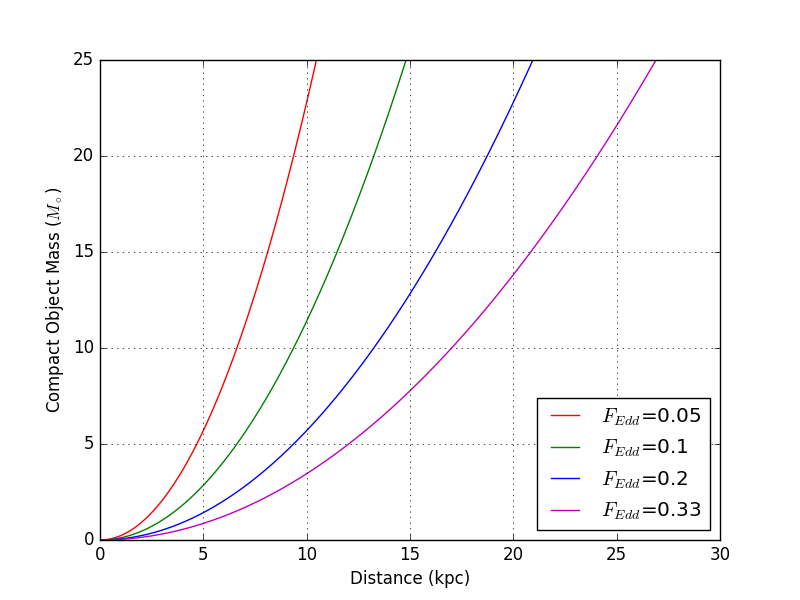
\includegraphics[width=\columnwidth, trim = 0mm 0mm 0mm 0mm]{images/MassDist.png}
    \captionsetup{singlelinecheck=off}
    \caption[Mass of the compact object in IGR J17091-3624 plotted against its distance, for values of peak Eddington fractions of $F_{Edd}=$0.05, 0.1, 0.2 and 0.33.]{Mass of the compact object in IGR J17091-3624 plotted against its distance, for values of peak Eddington fractions of $F_{Edd}=$0.05, 0.1, 0.2 and 0.33.}
   \label{fig:IGRMass}
\end{figure}

\subsection{Implications for Models of `Heartbeat' Variability}

\par I have found that hysteretic HID loops can execute in both directions in IGR J17091 (e.g. Section \ref{sec:Alta}), as well as found a revised estimate that IGR J17091 accretes at $\lesssim20$\% Eddington (Section \ref{sec:newmass}).  Both of these findings have implications for physical models of GRS 1915-like variability in this source.
\par Firstly, I find that Eddington-limited accretion is neither necessary nor sufficient for GRS 1915-like variability.  The discovery of GRS 1915-like variability in the sub-Eddington Rapid Burster \citep{Bagnoli_RB,Bagnoli_PopStudy} provided the first evidence that Eddington-limited accretion may not be a driving factor in this type of variability.  I strengthen this case by finding that IGR J17091-3624 is also likely sub-Eddington.  As such, I further rule out any scenario in which Eddington-limited accretion is required for GRS 1915-like variability in black hole LMXBs specifically.
\par Secondly, by using the direction of hysteretic HID loops, I find that hard photon lag in `heartbeat'-like classes of IGR J17091 can be either positive or negative.  This could mean that we must rule out the causal connection between soft and hard emission being common to all classes.
\par In either case, I find that scenarios that require high global accretion rates or predict a consistent hard photon lag (e.g. \citealp{Neilsen_GRSModel,Janiuk_Lag}), are not able to explain GRS 1915-like variability in IGR J17091 unless they also feature geometric obscuration in a subset of variability classes.  I note that simulations by \citealp{Nayakshin_GRSModel} require an Eddington fraction of $\gtrsim0.26$ before GRS 1915-like variability, a value which falls in the range $\sim0.05\mbox{--}0.33$ that I find for the peak Eddington fraction of IGR J17091.
\par In addition to being near its Eddington limit GRS 1915 also has the largest orbit of any known LMXB (e.g. \citealp{McClintock_BHBs}).  \citealp{Sadowski_MagField} have also shown that thin, radiation dominated regions of disks in LMXBs require a large-scale threaded magnetic field to be stable, and the field strength required to stabilise such a disk in GRS 1915 is higher than for any other LMXB they studied.  I suggest that one of these parameters is more likely to be the criterion for GRS 1915-like variability.  If better constraints can be placed on the disk size and minimum stabilising field strength in IGR J17091, it will become clear whether either of these parameters can be the unifying factor behind LMXBs that display GRS 1915-like variability.

\section{Conclusions}

\par I have constructed the first model-independent set of variability classes for the entire portion of the 2011--2013 outburst of IGR J17091 that was observed with \rxte .  I find that the data are well-described by a set of 9 classes;  7 of these appear to have direct counterparts in GRS 1915, while two are, so far, unique to IGR J17091.  \textsf{D.A.} and I find that variability in IGR J17091 is generally faster than in the corresponding classes of GRS 1915, and that patterns of quasi-periodic flares and dips form the basis of most variability in both objects.  Despite this, I find evidence that `heartbeat'-like variability in both objects may be generated by different physical processes.  In particular, while hard photons always lag soft in GRS 1915, I find evidence that hard photons can lag or precede soft photons in IGR J17091 depending on the variability class.
\par I also report on the long-term evolution of the 2011--2013 outburst of IGR J17091, in particular noting the presence of 3 re-flares during the later part of the outburst.  Using an empirical relation between hard-soft transition luminosity and Eddington luminosity \citep{Maccarone_2pct}, I estimate that IGR J17091 was likely accreting at no greater than $\sim33$\% of its Eddington limit at peak luminosity.
\par I use these results to conclude that any model of GRS 1915-like variability which requires a near-Eddington global accretion rate is insufficient to explain the variability we see in IGR J17091.  As such I suggest that an extreme value of some different parameter, such as disk size or minimum stabilising large-scale magnetic field, may be the unifying factor behind all objects which display GRS 1915-like variability.  This would explain why sub-Eddington sources such as IGR J17091 and the Rapid Burster do display GRS 1915-like variability, while other Eddington-limited sources such as GX 17+2 and V404 Cyg do not.

\cleardoublepage


\chapter{The Evolution of X-ray Bursts in the ``Bursting Pulsar'' GRO J1744--28}

\label{ch:BPbig}

\epigraph{\textit{The fountains of the great deep came bursting through, and the windows of heaven were open.}}{Genesis 7:11}
\vspace{1cm}

\par\noindent In Chapter \ref{ch:IGR}, I present a new way to classify variability in the LMXB IGR J17091-3624.  I compare this object with GRS 1915; although I find a number of differences between variability in the two systems, I conclude that the same broad phenomenon is likely behind variability in both.  I also find that IGR J17091 is likely significantly sub-Eddington during periods in which it displays GRS 1915-like variability.  This result can be seen as yet another piece of evidence that near-Eddington accretion is neither sufficient or necessary for GRS 1915-like behaviour.
\par To try and better constrain what does unite GRS 1915-like objects, the next step is to look for analogous behaviour in other systems.  As previously mentioned, \citet{Bagnoli_RB} reported variability similar to GRS 1915 in \textit{RXTE} lightcurves from the Rapid Burster.  As such the Rapid Burster, and its sister system the Bursting Pulsar, are natural places to look for evidence of GRS 1915-like variability.  Type II bursts seen in the Rapid Burster and the Bursting Pulsar are believed to be caused by viscous instabilities in the accretion disk \citep{Lewin_TypeII}, as is the X-ray variability seen GRS 1915 and IGR J17091.  However, as I discuss in Section \ref{sec:TIImod} the exact details of the mechanism responsible for Type II bursts remain unclear.
\par The Type II bursting behaviour in the Rapid Burster has been extensively studied (see e.g. \citealp{Lewin_TypeII,Hoffman_RB}).  \citet{Bagnoli_PopStudy} performed a full population study of all Type II bursts observed in this object by \textit{RXTE}.  Their results suggest that gating of the accretion by a strong magnetic field plays some role in the creation of Type II bursts: as this scenario requires a highly magnetised compact object, it cannot be employed to explain the variability seen in the black hole-primary GRS 1915 or IGR J17091.  To further probe the physics behind Type II X-ray bursts, in this chapter I perform a similar population study on bursts from the Bursting Pulsar.
\par Previous work by \citet{Giles_BP} indicated that Type II bursts in the 1995--1996 outburst of the Bursting Pulsar could be separated into a number of distinct populations based on peak flux.  This is a notable difference from the Rapid Burster, in which all Type II bursts have peak fluxes approximately equal to or less than object's Eddington Luminosity \citep{Tan_RBBursts}.  In this chapter I expand on the work of \citet{Giles_BP} and analyze \textit{RXTE}, \textit{NuSTAR}, \textit{Chandra}, \textit{XMM-Newton}, \textit{Swift} and \textit{INTEGRAL} data to fully quantify the population of Type II bursts in the Bursting Pulsar during all 3 outbursts in which they have been observed.  I study how the bursting in this object evolves over time throughout each outburst, and I link this behaviour to the long-term evolution of the source.  I also perform basic timing, morphology and spectral analysis on bursts, to try and understand the physical processes behind these phenomena.

\section{Data and Data Analysis}

\par Since discovery, the Bursting Pulsar has undergone three bright outbursts, which began in 1995, 1997 and 2014.  I refer to these outbursts as Outbursts 1, 2 and 3.  I do not consider the faint outburst in 2017 in this chapter \citep{Sanna_BPOutburst}, as no Type II bursts were observed during this time, nor do I analyse data taken while the source was in quiescence.  See \citet{Daigne_BPQ}, \citet{Wijnands_BPQ} and \citet{Degenaar_BPQuiescence} for studies of the Bursting Pulsar during quiescence.
\par I analysed data from all X-ray instruments which observed the Bursting Pulsar during these outbursts.  Specifically, I analysed lightcurves, the evolution of hardness ratios as a function of time and of count rate, and performed statistical analysis of properties associated with each individual burst.

\subsection{\textit{RXTE}}

\par I analysed data from \textit{RXTE}/PCA corresponding to the Outbursts 1 \& 2 of the Bursting Pulsar.  This in turn corresponded to observation IDs starting with 10401-01, 20077-01, 20078-01, 20401-01 and 30075-01, between MJDs 50117 and 51225.  This resulted in a total of 743\,ks of data over 300 observations, which I have listed in Appendix \ref{app:obs}. Lightcurve data were extracted from \texttt{fits} files using \texttt{FTOOLS}\footnote{\url{https://heasarc.gsfc.nasa.gov/ftools/ftools_menu.html}}.  Errors were calculated and quoted at the 1$\,\sigma$ level.
\par I also use data from the \textit{RXTE}/ASM to monitor the long-term evolution of the source.  ASM data were taken from MIT's ASM Light Curves Overview website\footnote{\url{http://xte.mit.edu/ASM_lc.html}}.

\subsubsection{Long-Term Evolution}

\par To analyse the long-term evolution of the source during its outbursts, I extracted 2--16\,keV count rates from the \textit{Standard2} data in each observation.  Following \citet{Altamirano_CrabNorm}, I normalised the intensity estimated in each observation by the intensity of the Crab nebula, using the Crab observation that is the closest in time but within the same PCA gain epoch as the observation in question (see \citealp{Jahoda_Calibrate}).

\subsubsection{Burst Identification and Analysis}

\label{sec:burst_diff}

\par To perform population studies on the Type II bursts in the Bursting Pulsar, I first extracted lightcurves from the \texttt{Standard1} data in each observation, as this data is available for all \textit{RXTE} observations.  I used my own \texttt{PANTHEON} software to search these lightcurves and return a list of individual bursts, using the algorithm described in Section \ref{sec:Flares}.  I manually cleaned spurious detections from my sample.  I defined a `burst' as an event that lasted at least 3 seconds during which the 1\,s binned count rate exceeded 3 standard deviations above the persistent emission level and reached a maximum of at least five standard devations above the persistent emission level.  I did not subtract background, as all count rate-related parameters I analyse are persistent emission subtracted, automatically removing background contribution.
\par During the analysis, Arianna Albayati (\textsf{A.A.}) and I discovered a number of different ``classes'', similar to the multiple classes of burst described by \citet{Giles_BP}.  Our classes varied significantly in terms of overall structure, and as such needed to be treated separately; I show representative lightcurves from each of our classes in Figure \ref{fig:classes}.  These classes were separated from one another by a number of criteria including peak count rate and recurrence time (the time between peaks of consecutive bursts).
\par The vast majority of detected bursts resembled the Type II seen in the Rapid Burster (referred to as `Normal Bursts' in Section \ref{sec:Results}) in terms of shape, duration and amplitude.  I rebinned the data corresponding to these Normal Bursts to 0.5\,s.  I sampled the persistent emission before the burst, and defined the start of the burst as the first point at which count rate exceeded 5 standard deviations above the persistent emission before the burst.  The end of the burst was defined similarly, but instead sampling the persistent emission after the burst; by doing this, I avoid making the implicit assumption that the persistent emission is equal before and after the burst.  I fitted phenomenologically-motivated lightcurve models to each of these bursts (described in detail in Section \ref{sec:struc}), and used these fits to extract a number of parameters which characterise the shape and energetics of a burst (such as burst duration, total photon counts associated with a burst and persistent emission count rate).
\par Due to the high peak count rates of Normal Bursts, data were affected by dead-time (compare e.g. \textit{GRANAT} data presented in \citealp{Sazonov_BPGranat}).  I calculate the approximate Dead-Time Factors (DTFs) for a number of the brightest Normal Bursts in my sample, using 1\,s binned data, using the following formula in the \textit{RXTE} Cookbook\footnote{\url{https://heasarc.gsfc.nasa.gov/docs/xte/recipes/pca_deadtime.html}}:
\begin{equation}
\Delta=\frac{C_{Xe}+C_{Vp}+C_{Rc}+15C_{VL}}{N_{PCU}}\times10^{-5}
\end{equation}
Where $\Delta$ is the fractional detector deadtime, $C_{Xe}$ is the Good Xenon count rate, $C_{Vp}$ is the coincident event count rate, $C_{Rc}$ is the propane layer count rate, $C_{VL}$ is the very large event count rate and $N_{PCU}$ is the number of PCUs active at the time.
\par I estimate that dead-time effects reduce the peak count rates by no more than $\sim12$\%; however, due to the sharply-peaked nature of bursts from the Bursting Pulsar, the deadtime effect depends on the binning used.  Due to this ambiguity I do not correct for dead-time in Normal Bursts.  The dead-time corrections required for the count rates seen in other classes of burst are minimal, as they are orders of magnitude fainter \citep{Giles_BP}.
\par To test for correlations between parameters in a model-independent way, I used the Spearman's Rank correlation coefficient (as available in \texttt{Scipy}, \citealp{NumPy}).  This metric only tests the hypothesis that an increase in the value of one parameter is likely to correspond to an increase in the value of another parameter, and it is not affected by the shape of the monotonic correlation to be measured.  Although dead-time effects lead to artificially low count rates being reported, a higher intensity still corresponds to a higher reported count rate.   As such, using this correlation coefficient removed the effects of dead-time on my detection of any correlations.
\par To calculate the distribution of recurrence times between consecutive bursts, I considered observations containing multiple bursts.  If fewer than 25\,s of data gap exists between a pair of bursts, I considered them to be consecutive and added their recurrence time to the distribution.  I choose this maximum gap size as this is approximately the timescale over which a Normal Burst occurs.
\par When \texttt{SB\_62us\_0\_23\_500ms} and \texttt{SB\_62us\_24\_249\_500ms} mode data were available, I divided my data into two energy bands: A (PCA channels 0--23, corresponding to $\sim2$--$7$\,keV\footnote{In \textit{RXTE} gain epoch 1, corresponding to dates before MJD 50163.  This corresponds to $\sim2$--$9$\,keV in epoch 2 (MJDs 50163--50188) and $\sim2$--$10$\,keV in epoch 3 (MJDs 50188--51259).}) and B (channels 24--249, corresponding to $\sim8$--$60$\,keV\footnote{In \textit{RXTE} gain epoch 1.  This corresponds to $\sim9$--$60$\,keV in epoch 2 and $\sim10$--$60$\,keV in epoch 3.}).  The evolution of colour (defined as the ratio of the count rates in B and A) throughout a burst could then be studied.  Due to the very high count rates during Normal Bursts, I did not correct for background.  During fainter types of burst I estimate the background in different energy bands by subtracting count rates from \textit{RXTE} observation 30075-01-26-00 of this region, when the source was inactive.  Unlike using the \textit{RXTE} background model, this method subtracts the contributions from other sources in the field.  However, as it is unclear whether any of the rest of these sources are variable, the absolute values of colours I quote should be treated with caution.  I created hardness-intensity diagrams to search for evidence of hysteretic loops in hardness-intensity space.
\par Following \citet{Bagnoli_PopStudy}, I used the total number of persistent emission-subtracted counts as a proxy for fluence for all bursts other than Normal Bursts.  As the contribution of the background does not change much during a single observation, this method also automatically subtracts background counts from my results.

\subsubsection{Detecting Pulsations}

\par The Bursting Pulsar is situated in a very dense region of the sky close to the Galactic centre, and so several additional objects also fall within the 1$^\circ$ \textit{RXTE}/PCA field of view.  Therefore it is important to confirm that the variability I observe in my data does in fact originate from the Bursting Pulsar.
\par To ascertain that all bursts considered in this study are from the Bursting Pulsar, Dr. Andrea Sanna (\textsf{A.S.}) analysed the coherent X-ray pulse at the pulsar spin frequency to confirm that the source was active.  \textsf{A.S.} first corrected the photon time of arrivals (ToA) of the \textit{RXTE} PCA dataset, and barycentred this data using the \texttt{faxbary} tool (DE-405 Solar System ephemeris).  \textsf{A.S.} corrected for the binary motion by using the orbital parameters reported by \citet{Finger_Pulse}.
\par For each PCA observation \textsf{A.S.} investigated the presence of the $\sim 2.14$\,Hz coherent pulsation by performing an epoch-folding search of the data using 16 phase bins and starting with the spin frequency value $\nu=2.141004$ Hz, corresponding to the spin frequency measured from the 1996 outburst of the source \citep{Finger_Pulse}, with a frequency step of $10^{-5}$\,Hz for 10001 total steps. \textsf{A.S.} detected X-ray coherent pulsations in all PCA observations performed during Outbursts 1 \& 2.

\subsection{\textit{Swift}}
\par In this study, I made use of data from XRT and BAT \textit{Swift}.  I extracted a long-term 0.3--10\,keV \textit{Swift}/XRT lightcurve of Outburst 3 using the lightcurve generator provided by the UK Swift Science Data Centre (UKSSDC, \citealp{Evans_Swift1}).  I also make use of \textit{Swift}/BAT lightcurves from the Swift/BAT Hard X-ray Transient website\footnote{\url{https://swift.gsfc.nasa.gov/results/transients/}} (see \citealp{Krimm_BAT}).

\subsection{\textit{INTEGRAL}}

\par I also made use of data from IBIS aboard \textit{INTEGRAL}.  I extracted 17.3--80\,keV IBIS/ISGRI lightcurves of the Bursting Pulsar during Outburst 3 using the \textit{INTEGRAL} Heavens portal.  This is provided by the \textit{INTEGRAL} Science Data Centre \citep{Lubinski_Heavens}.

\subsection{\textit{Chandra}}

\par The Bursting Pulsar was targeted with \textit{Chandra} three times during Outburst 3 (Table \ref{tab:Chandra}).  One of these observations (OBSID 16596) was taken simultaneously with a \textit{NuSTAR} observation (80002017004).  In all three observations data were obtained with the HETG, where the incoming light was dispersed onto the ACIS-S array. The ACIS-S was operated in continued clocking (CC) mode to minimize the effects of pile-up. The  Chandra/HETG observations were analysed using standard tools available within \texttt{ciao} v. 4.5 \citep{Fruscione_Ciao}. Dr. Nathalie Degenaar (\textsf{N.D.}) extracted 1\,s binned light curves from the \texttt{evt2} data using \texttt{dmextract}, where the first order positive and negative grating data from both the Medium Energy Grating (MEG; 0.4-5 keV) and the High Energy Grating (HEG; 0.8--8\,keV) were combined.

\begin{table}
\centering
\begin{tabular}{lllllll}
\hline
\hline
\scriptsize  OBSID &\scriptsize Exposure (ks) &\scriptsize MJD &\scriptsize Reference \\
\hline
16596  	& 10 &  56719      &   \citet{Younes_Expo} \\
16605  	& 35 &   56745    &    \citet{Degenaar_BPSpec}\\
16606  	& 35 &   56747    &    \citet{Degenaar_BPSpec}\\
\hline
\hline
\end{tabular}
\caption[Information on the three \textit{Chandra} observations of the Bursting Pulsar during Outburst 3.]{Information on the three \textit{Chandra} observations of the Bursting Pulsar during Outburst 3.  All other observations of the Bursting Pulsar in the Chandra archive were obtained at times that the source was in quiescence.}
\label{tab:Chandra}
\end{table}

\subsection{\textit{XMM-Newton}}

\par A single pointed \textit{XMM-Newton} observation of the Bursting Pulsar was taken during Outburst 3 on MJD 56722 (OBSID 0729560401) for 85\,ks.  I extracted a 0.5--10\,keV lightcurve from EPIC-PN at 1\,s resolution using \texttt{xmmsas} version 15.0.0.  During this observation, EPIC-PN was operating in Fast Timing mode.  I use EPIC-PN as the statistics are better than in MOS1 or MOS2.

\subsection{\textit{Suzaku}}
\par \textit{Suzaku} observed the Bursting Pulsar once during Outburst 3 on MJD 56740 (OBSID 908004010).  To create a lightcurve, \textsf{K.Y.} reprocessed and screened data from the X-ray Imaging Spectrometer (XIS, \citealp{Koyama_XIS})using the \texttt{aepipeline} script and the latest calibration database released on June 7, 2016.  The attitude correction for the thermal wobbling was made by \texttt{aeattcor2} and \texttt{xiscoord} \citep{Uchiyama_SuzPSF}. The source was extracted within a radius of 250 pixels corresponding to 260'' from the image center.  The background was extracted from two regions near either end of the XIS chip, and subtracted from the source.

\subsection{\textit{NuSTAR}}

\par \textit{NuSTAR} observed the Bursting Pulsar three times during its outbursts, all times in Outburst 3.  One of these observations was taken while the Bursting Pulsar was not showing X-ray bursts, and the other two are shown in Table \ref{tab:NuS}.  I extracted lightcurves from both of these observations using \texttt{nupipeline} and \texttt{nuproducts}, following standard procedures\footnote{See \url{https://www.cosmos.esa.int/web/xmm-newton/sas-threads}.}.

\begin{table}
\centering
\begin{tabular}{lllllll}
\hline
\hline
\scriptsize  OBSID &\scriptsize Exposure (ks) &\scriptsize MJD &\scriptsize Reference \\
\hline
80002017002 	& 29 & 56703 &  \citet{Dai_Hlags}  \\
80002017004 	& 9 & 56719 & \citet{Younes_Expo}\\
\hline
\hline
\end{tabular}
\caption[Information on two \textit{NuSTAR} observations of the Bursting Pulsar.]{Information on the two \textit{NuSTAR} observations of the Bursting Pulsar during the main part of Outburst 3.}
\label{tab:NuS}
\end{table}

\section{Results}
\label{sec:Results}

\subsection{Outburst Evolution}

\par I show the long-term monitoring lightcurves of Outbursts 1, 2 and 3 in Figure \ref{fig:global_ob}, as well as mark the dates of pointed observations with various instruments.

\begin{figure}
  \centering
  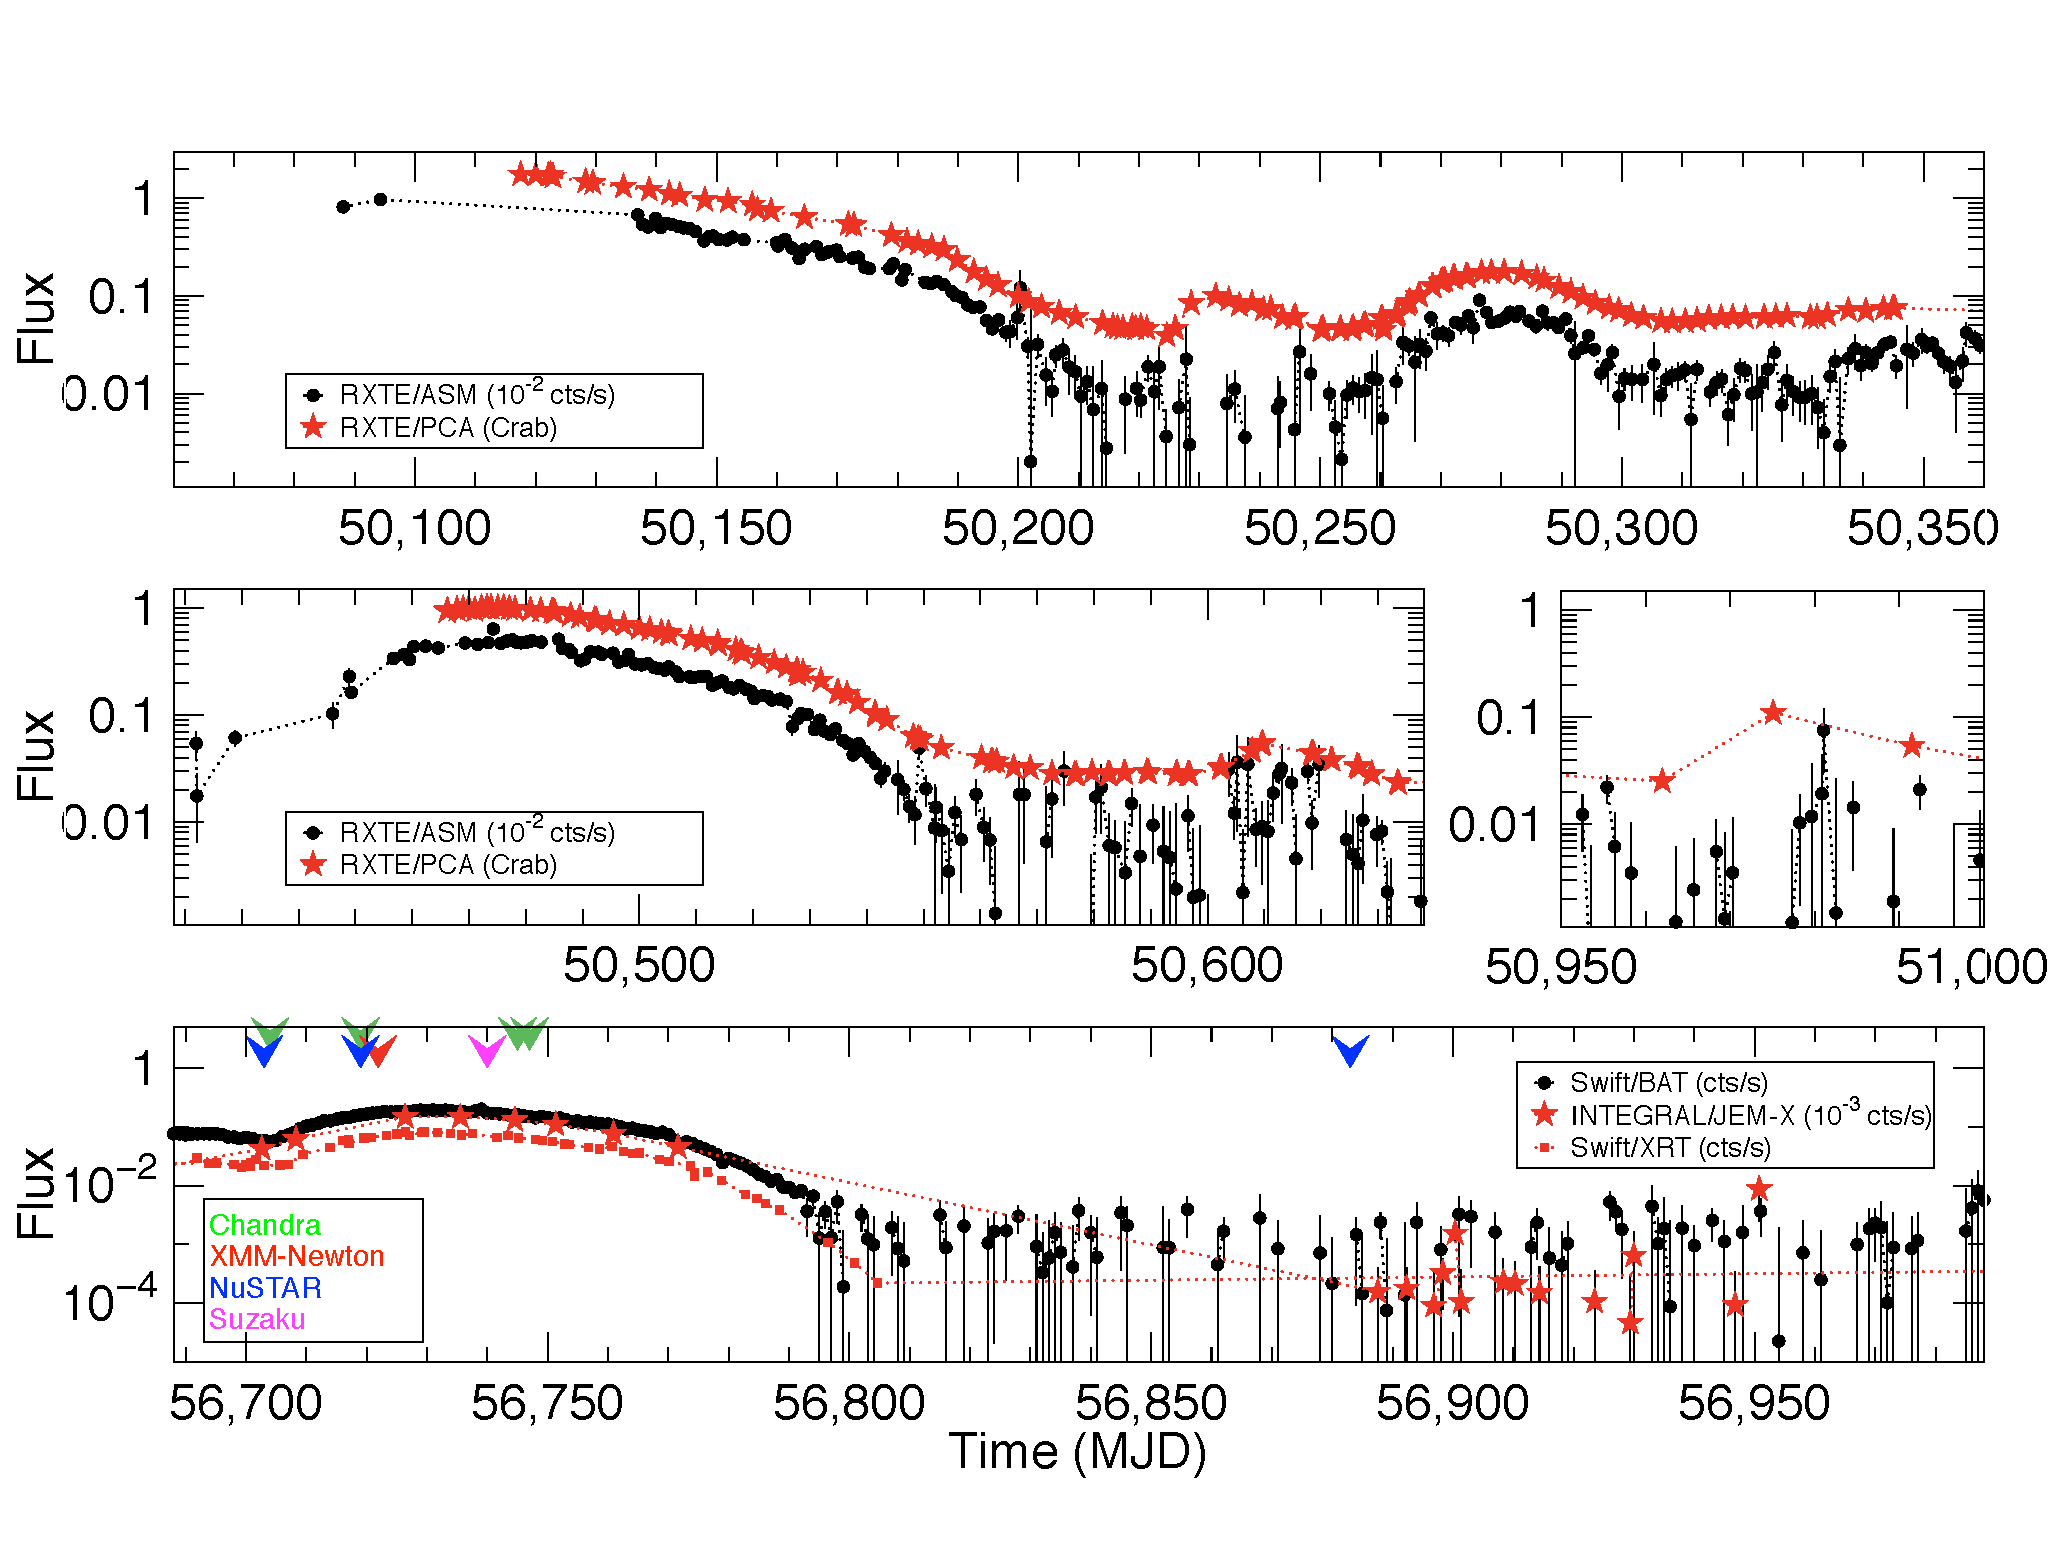
\includegraphics[width=.9\linewidth, trim={0cm 0 0cm 0},clip]{images/lc_comp.pdf}
  \caption[Comparisons of three outbursts of the Bursting Pulsar.]{\small Comparisons of the three outbursts of the Bursting Pulsar reported on in this chapter.  Times corresponding to pointed observations with \textit{Chandra}, \textit{NuSTAR}, \textit{Suzaku}, \textit{Swift} and \textit{XMM-Newton} are marked.}
  \label{fig:global_ob}
\end{figure}

\par The Bursting Pulsar was discovered already in outburst on December 12 1995 \citep{Fishman_Discovery}; BATSE data suggest that this outburst began several days earlier on December 3 \citep{Paciesas_BPDiscovery,Bildsten_Rev}.  The main outburst ended around May 10 1996 \citep{Woods_PulseBursts}.  I show the global lightcurve of this outburst in Figure \ref{fig:global_ob}, Panel 1.  As \textit{RXTE} did not observe the object before or during the peak of Outburst, I can only obtain a lower limit of $\sim1.75$\,Crab for the peak 2--16\,keV flux.
\par There are at least two major rebrightening events in the tail of Outburst 1, which can be seen clearly  in Figure \ref{fig:global_ob} centred at MJDs of $\sim50235$ and $\sim50280$.  During these rebrightening events, the 2--16\,keV flux peaked at $\sim0.10$ and $\sim0.18$\,Crab respectively.

\par Outburst 2 began on December 1 1996 and ended around April 7 1997 \citep{Woods_OB2}.  The 2--16\,keV flux peaked at 1.02\,Crab on MJD 50473; I show the global lightcurve of this outburst in Figure \ref{fig:global_ob}, Panel 2.  Type II bursts are seen in \textit{RXTE}/PCA lightcurves from Outburst 2 between MJDs 50466 and 50544.  One rebrightening event occurred during the tail of Outburst 2, centred at an MJD of $\sim50615$ with a peak 2--16\,keV flux of $\sim54$\,mCrab.  A second possible rebrightening event occurs at MJD 50975, with a peak 2--16\,keV flux of 11\,mCrab, but the cadence of \textit{RXTE}/PCA observations was too low to unambiguously confirm the existence of a reflare at this time.

\par Outburst 3 began on January 31, 2014 \citep{Negoro_OB3,Kennea_BPOutburst} and ended around April 23 (e.g. \citealp{Dai_OB3}).  The daily 0.3--10\,keV Swift/XRT rate peaked at 81\,cts\,s$^{-1}$ on MJD 56729, corresponding to 0.4\,Crab.  I show the global lightcurve of this outburst in Figure \ref{fig:global_ob}, Panel 3.
\par During the main part of Outburst 3, \textit{Swift}, \textit{XMM-Newton} and \textit{Suzaku} made one pointed observation each, \textit{Chandra} made four observations, and \textit{NuSTAR} made three observations.  The \textit{Chandra} observation on March 3 2014 was made simultaneously with one of the \textit{NuSTAR} observations (see \citealp{Younes_Expo}).  After the main part of the outburst, the source was not well-monitored, although it remained detectable by \textit{Swift}/BAT, and it is unclear whether any rebrightening events occured.  A single \textit{NuSTAR} observation was made during the outburst tail on August 14 2014.

\par As can be seen in Figure \ref{fig:global_ob}, the main section of all three outburst follow a common profile, over a timescale of $\sim150$ days.  A notable difference between outbursts 1 \& 2 is the number of rebrightening events; while I find two rebrightening events associated with Outburst 1, I only find one associated with Outburst 2 unless I assume the event at MJD 50975 is associated with the outburst.  Additionally, Outburst 2 was at least a factor $\sim1.7$ fainter at its peak than Outburst 1 (see also \citealp{Woods_OB2}), while Outburst 3 was a factor of $\gtrsim4$ fainter at peak than Outburst 1.

\subsubsection{Pulsations}

\par \textsf{A.S.} found pulsations in PCA data throughout the entirety of Outbursts 1 \& 2.  This confirms that the Bursting Pulsar was active as an X-ray pulsar in all of my observations, leading us to conclude that all the types of Type II bursts we see are from the Bursting Pulsar.  In Figure \ref{fig:pulsovertime}, I show that the amplitude of these pulsations approximately followed the intensity of the source in both outbursts, but there were significant deviations from this trend.  These deviations will require further investigation, and a comparison with other accreting pulsar systems.  Previous studies have shown that pulsations were also present during Outburst 3 (e.g. \citealp{Sanna_BP}).

\begin{figure}
  \centering
  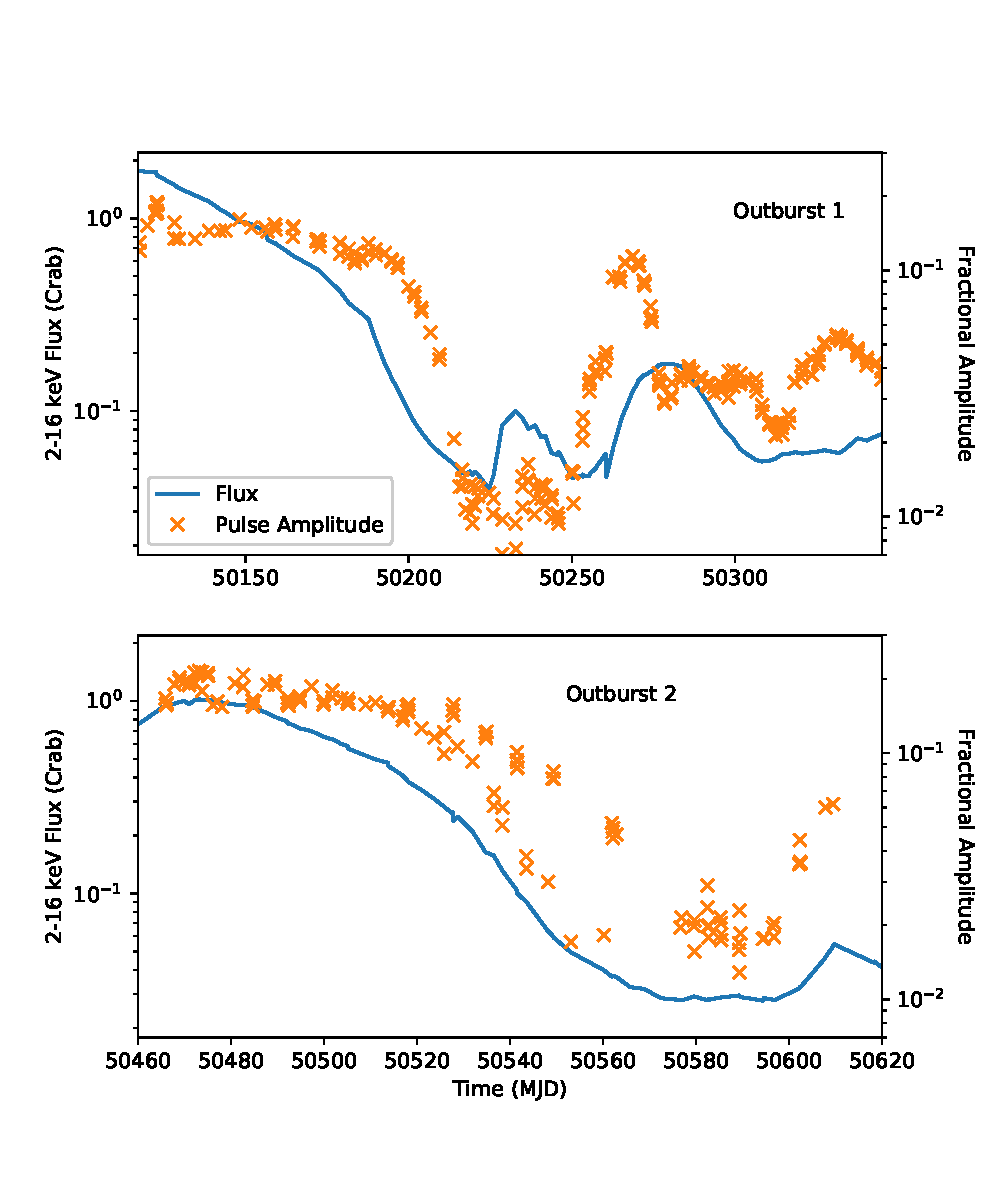
\includegraphics[width=.9\linewidth, trim={0.4cm 1cm 0cm 1cm},clip]{images/PulseAmp.eps}
  \caption[\textit{RXTE}/PCA lightcurves of Outbursts 1 \& 2 of the Bursting Pulsar, overlaid with plots showing how the fractional RMS of the 2.4\,Hz pulsation changes as a function of time.]{\small 2--16\,keV \textit{RXTE}/PCA lightcurves of Outbursts 1 \& 2 of the Bursting Pulsar (solid blue), overlaid with plots showing how the fractional RMS of the 2.4\,Hz pulsation associated with the pulsar changes as a function of time during these outbursts (orange crosses).}
  \label{fig:pulsovertime}
\end{figure}

\subsubsection{Bursting Behaviour}

\label{sec:bburstevo}

\par Bursts are seen in \textit{RXTE}/PCA lightcurves from the start of the Outburst 1 (e.g. \citealp{Kouveliotou_BP}).  These Type II bursts occur until around MJD 50200, as the source flux falls below $\sim0.1$\,Crab in the 2--16\,keV band.  
\par During the latter part of the first rebrightening after Outburst 1, between MJDs 50238 and 50246, \textsf{A.A.} found Type II-like bursts with amplitudes $\sim2$ orders of magnitude smaller than those found during the main outburst event.  These gradually increased in frequency throughout this period of time until evolving into a period of highly structured variability which persisted until MJD 50261.
\par In Outburst 2, Type II bursts occured between MJDs $\sim50466$ and $50542$.  Low-amplitude Type II-like bursts were seen during the latter stages of the main outburst, between MJDs 50562 and 50577.  These again evolved into a period of highly structured variability; this persists until MJD 50618, just after the peak of the rebrightening event.
\par High-amplitude Type II bursts were also seen in Outburst 3 (e.g. \citealp{Linares_NewBurst}).  As no soft ($\lesssim10\,$keV) X-ray instrument was monitoring the Bursting Pulsar during the latter part of Outburst 3, it is unknown whether this Outburst showed the lower-amplitude bursting behaviour seen at the end of Outbursts 1 \& 2.  Low amplitude bursting behaviour is not seen in the pointed \textit{NuSTAR} observation which was made during this time.

\subsection{Categorizing Bursts}

\label{sec:classes}

\par \textsf{A.A.} and I found that bursts in the Bursting Pulsar fall into a number of discrete classes, lightcurves from which I show in Figure \ref{fig:classes}.  These classes are as follows:

\begin{figure}
  \centering
  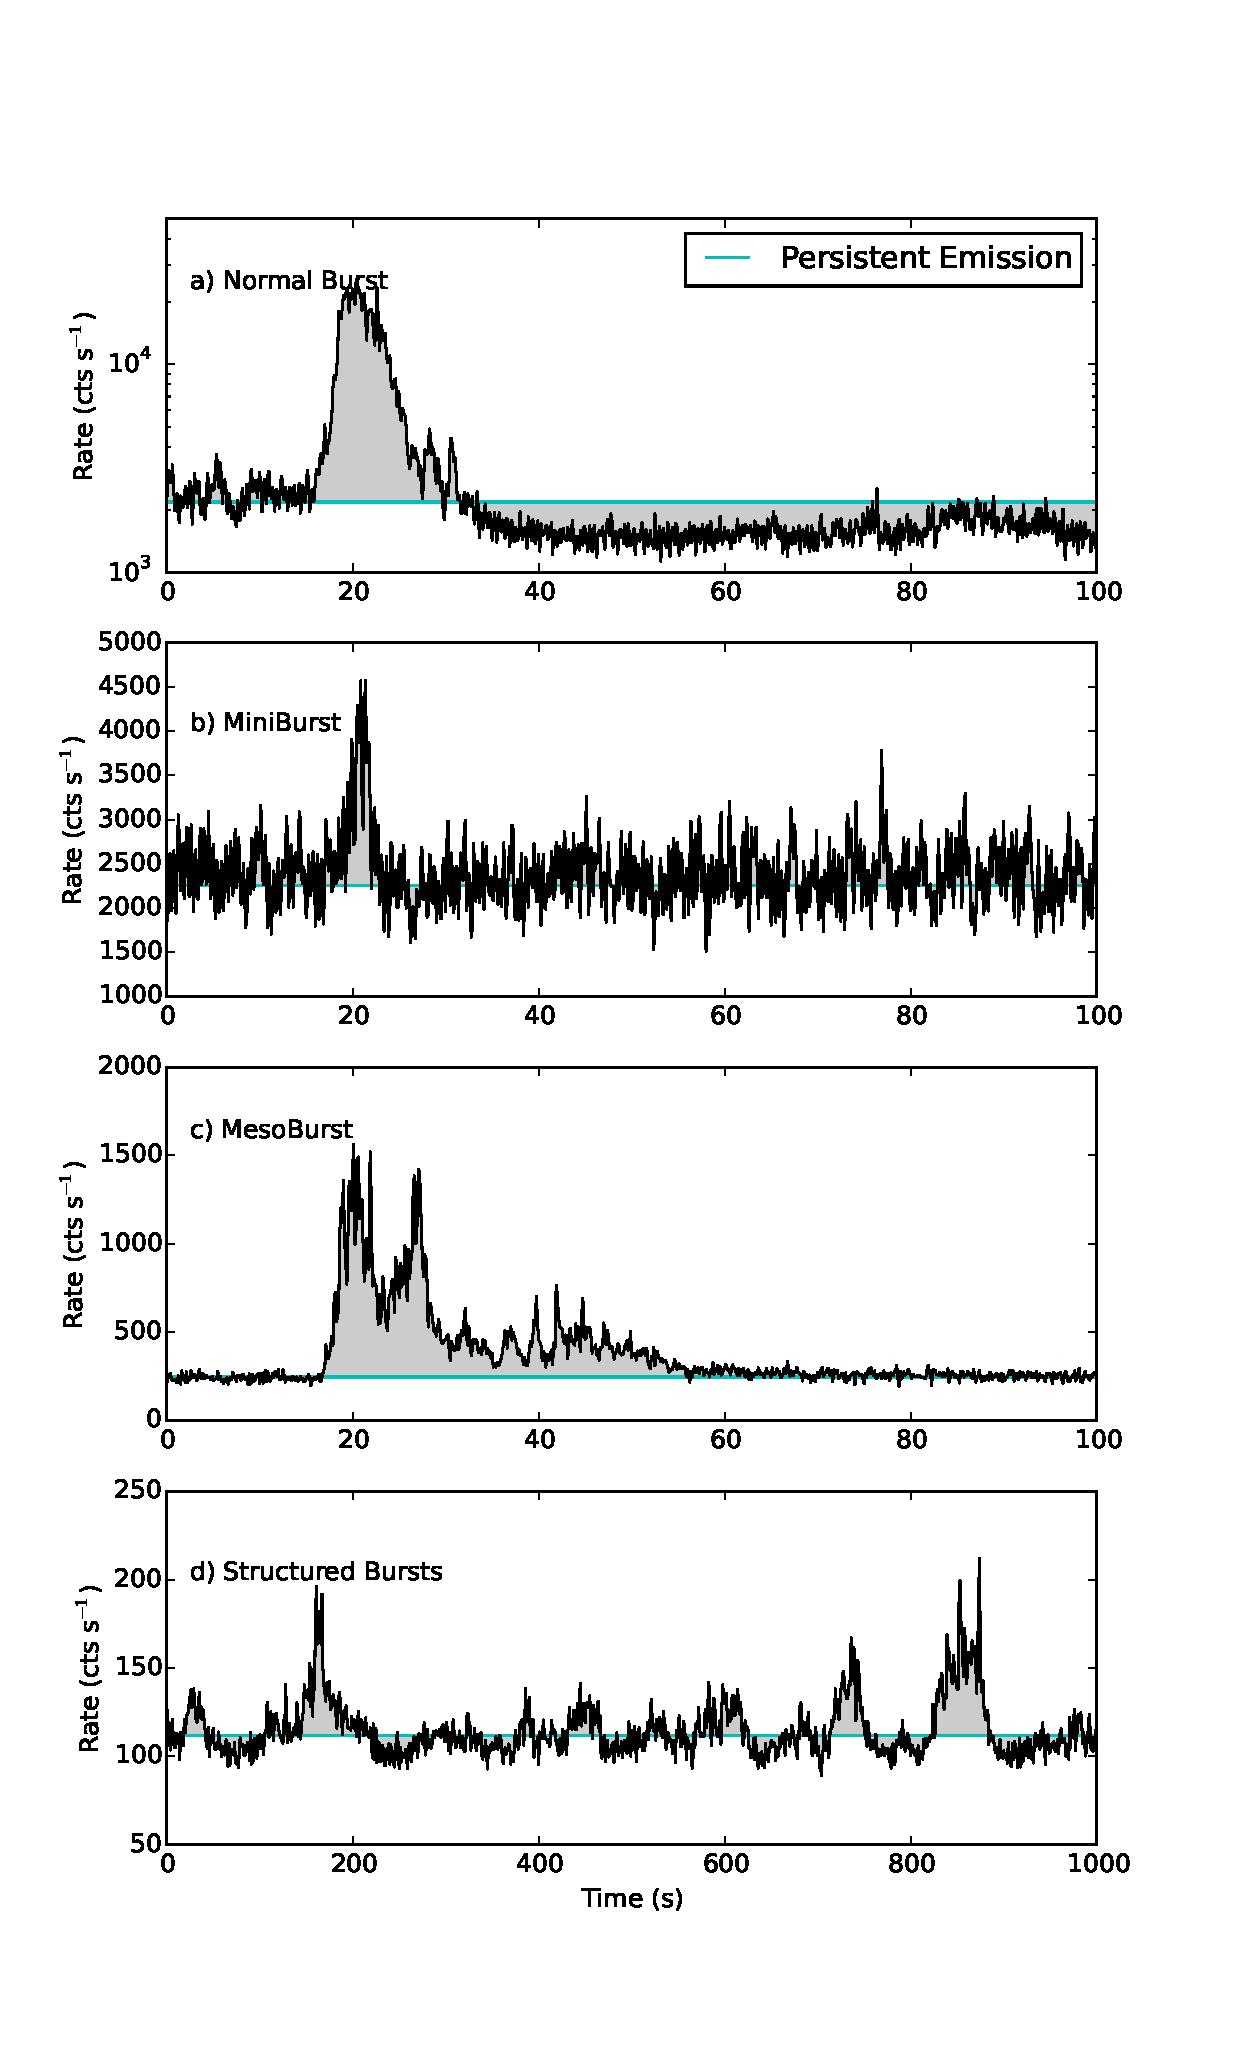
\includegraphics[width=.9\linewidth, trim={0.7cm 2.1cm 1.5cm 3.4cm},clip]{images/comp_bursts.eps}
  \caption[Lightcurves for the four classes of bursting behaviour identified in the Bursting Pulsar.]{\small 2--49\,keV lightcurves for the four classes of bursting behaviour identified in this chapter: \textbf{a)} Normal Burst, \textbf{b)} Miniburst, \textbf{c)} Mesoburst, \textbf{d)} Structured Bursts.  Note that Panel \textbf{d} is plotted with a different time scaling to the other panels so as to better show the behaviour of Structured Bursting.  On all figures the median count rate, which I use as a proxy for the persistent emission, is plotted in cyan.  Lightcurves \textbf{a}-\textbf{c} are binned to 0.125\,s, while lightcurve \textbf{d} is binned to 1\,s.}
  \label{fig:classes}
\end{figure}

\begin{itemize}
\item Normal Bursts (Figure \ref{fig:classes}, Panel a): the brightest bursts seen from this source, with peak count 1\,s binned rates of $\sim10000$\,cts\,s$^{-1}$\,PCU$^{-1}$, and recurrence timescales of order $\sim1000$\,s.  These bursts are roughly Gaussian in shape with durations of $\sim10$\,s, and are followed by a `dip' in the persistent emission count rate with a duration of order 100\,s (see also e.g. \citealp{Giles_BP}).
\item Minibursts (Figure \ref{fig:classes}, Panel b): faint bursts with 1\,s-binned peak count rates of $\sim2$ times the persistent emission count rate.  Minibursts are variable, with duration timescales between $\sim5$--50\,s.  These bursts are also sometimes followed by dips similar to those seen after Normal Bursts.
\item Mesobursts (Figure \ref{fig:classes}, Panel c): Type II-like bursts.  These bursts differ from Normal Bursts in that they do not show well-defined subsequent `dips'.  They are also fainter than Normal Bursts, with peak count 1\,s binned count rates of $\sim1000$\,cts\,s$^{-1}$\,PCU$^{-1}$.  Their burst profiles show fast rises on timescales of seconds, with slower decays and overall durations of $\sim50$\,s.  The structure of the bursts is very non-Gaussian, appearing as a small forest of peaks in lightcurves.
\item Structured Bursts (Figure \ref{fig:classes}, Panel d): the most complex class of bursting behaviour we observe from the Bursting Pulsar, consisting of patterns of flares and dips in the X-ray lightcurve.  The amplitudes of individual flares are similar to those of the faintest Mesobursts.  The recurrence timescale is of the order of the timescale of an individual flare, meaning that is it difficult to fully separate individual flares of this class.
\end{itemize}

\par In the upper panel of Figure \ref{fig:jointhist} I show a histogram of persistent-emission-subtracted peak count rates for all Normal and Mesobursts observed by \textit{RXTE}.  I split these two classes based on the bimodal distribution in peak count rate as well as the lack of dips in Mesobursts.
\par In the lower panel of Figure \ref{fig:jointhist}, I show the histogram of peak count rates for all Normal and Minibursts observed by \textit{RXTE} as a fraction of the persistent emission at that time.  I split these two classes based on the strongly bimodal distribution in fractional amplitude.

\begin{figure}
  \centering
  \includegraphics[width=.8\linewidth, trim={1.3cm 0.4cm 2.0cm 0.8cm},clip]{images/norm_meso_sep.eps}
  \includegraphics[width=.8\linewidth, trim={1.3cm 0.4cm 2.0cm 0.8cm},clip]{images/norm_mini_sep.eps}
  \caption[Histogram of the peak 1\,s binned peak count rates during Normal Bursts, Mesobursts and Minibursts as seen by \textit{RXTE}]{\small \textbf{Upper Panel:} A histogram of the peak 1\,s binned peak count rates of the joint population of all Normal and Mesobursts seen by \textit{RXTE}.  The dashed line indicates the position of the threshold above which I consider a Type II-like burst to be a Normal Burst.  The resultant split of the population into Normal and Mesobursts is indicated by blue and red shading respectively.  The skewed shape of the distribution of Normal Bursts is due to the effects of dead-time putting an effective cap on their maximum observed intensity.
 \textbf{Lower Panel:} A histogram of the peak 1\,s binned peak count rates of the joint population of all Normal and Minibursts seen by \textit{RXTE}, divided by the persistent emission count rate at that time.  The dashed line indicates the position of the threshold below which I consider a burst to be a Miniburst.  The resultant split of the population into Normal and Minibursts is indicated by blue and green shading respectively.
  Note that the $x$-axis of both plots is logarithmic, and so number density is not preserved.}
  \label{fig:jointhist}
\end{figure}

\par I also find 6 bursts with fast ($\sim1$\,s) rises and exponential decays that occur during the lowest flux regions of the outburst ($\lesssim50$\,mCrab).  \citet{Strohmayer_BPFieldTypeI} and \citet{Galloway_TypeI} have previously identified these bursts as being Type I X-ray bursts from another source in the \textit{RXTE} field of view.  To show that these unrelated Type I bursts would not be confused with Minibursts, I add examples of the Type I bursts to lightcurves from observations containing Minibursts.  I find that the peak count rates in Type I bursts are roughly equal to the amplitude of the noise in the persistent flux in these observations, hence they would not be detected by my algorithms.
\par I show when in Outbursts 1 \& 2 each type of burst was observed in Figures \ref{fig:ob_evo1} and \ref{fig:ob_evo2} respectively.  Normal Bursts and Minibursts (red) occur during the same periods of time from around the peak of an outburst until the persistent emission falls beneath $\sim0.1$\,Crab; assuming an Eddington Limit of $\sim1$\,Crab (e.g \citealp{Sazonov_BPGranat}), this corresponds to an Eddington ratio of $\sim0.1$.  After this point, bursting is not observed for a few tens of days.  Mesobursts (blue) begin at the end of a rebrightening event in Outburst 1 and during the final days of the main part of the outburst in Outburst 2.  Structured Bursts (yellow) occur during the first part of a rebrightening event in both outbursts.  Although there was a second rebrightening event after Outburst 1, neither Mesobursts nor Structured Bursts were observed at this time.  Based on this separation, as well as differences in structure, I treat each class of burst separately below.

\begin{figure}
  \centering
  \includegraphics[width=.9\linewidth, trim={9.5cm 0cm 10cm 0cm},clip]{images/obevo1.pdf}
  \caption[Lightcurve of the 1995--1996 outburst of the Bursting Pulsar, highlighting periods of time during which Mesobursts, Structured Bursts or Normal and Mini bursts are observed.]{\small Central panel shows the global 2--16\,keV \textit{RXTE}/PCA lightcurve of the 1995--1996 outburst of the Bursting Pulsar, highlighting periods of time during which Mesobursts (blue) Structured Bursts (yellow) or Normal and Mini bursts (red) are observed.  A single Mesoburst was also observed on MJD 50253, during the period of the outburst highlighted in yellow (see Figure \ref{fig:meso_in_struc}).  Other panels show example lightcurves which contain the aforementioned types of bursting behaviour.  See section \ref{sec:classes} for a detailed treatment of burst classification.  Fluxes reported in units of Crab.}
  \label{fig:ob_evo1}
\end{figure}

\begin{figure}
  \centering
  \includegraphics[width=.9\linewidth, trim={9.5cm 0cm 10cm 0cm},clip]{images/obevo2.pdf}
  \caption[Lightcurve of the 1997--1999 outburst of the Bursting Pulsar, highlighting periods of time during which Mesobursts, Structured Bursts or Normal and Mini bursts are observed.]{\small Central panel shows the global 2--16\,keV \textit{RXTE}/PCA lightcurve of the 1997--1999 outburst of the Bursting Pulsar, highlighting periods of time during which Mesobursts (blue) Structured Bursts (yellow) or Normal and Mini bursts (red) are observed.  Other panels show example lightcurves which contain the aforementioned types of bursting behaviour.}
  \label{fig:ob_evo2}
\end{figure}

\subsection{Normal Bursts}

\par I define Normal Bursts as the set of all bursts with a persistent-emission-subtracted peak 1\,s binned \textit{RXTE}/PCA-equivalent count rate above 3000\,cts\,s$^{-1}$\,PCU$^{-1}$.  Normal Bursts account for 99 out of the 190\footnote{This number does not include Structured Bursts as their complex structure makes them difficult to separate.} bursts identified for this study.  They are observed during all three outbursts covered in this study.  They occurred between MJDs 50117 and 50200 in Outburst 1, and between 50466 and 50542 in Outburst 2; during these intervals, \textit{RXTE} observed the source for a total of 192\,ks.  See Table \ref{tab:staretimes} to compare these with numbers for the other classes of burst identified in this study.  Normal Bursts occur during the same time intervals in which Minibursts are present.  In both of these outbursts, the region of Normal and Minibursts correspond to the time between the peak of the outburst and and the time that the persistent intensity falls below $\sim0.1$\,Crab.

\begin{table}
\centering
\begin{tabular}{llll}
\hline
\hline
\scriptsize  Bursting Mode &\scriptsize Bursts &\scriptsize Total Exposure (ks) &\scriptsize Duration (d) \\
\hline
Normal Bursts & 99  & 192 & 76\\
Minibursts & 48 & 192  & 76\\
Mesobursts & 43 &44 &25\\
Structured Bursts & - &80 &54 \\
\hline
\hline
\end{tabular}
\caption[Statistics on the population of Normal Bursts in Outbursts 1 and 2 of the Bursting Pulsar.]{Statistics on the population of bursts I use for this study, as well as the duration and integrated \textit{RXTE}/PCA exposure time of each mode of bursting.  All numbers are the sum of values for Outbursts 1 and 2.  As Normal and Minibursts happen during the same period of time in each outburst, the exposure time and mode duration for these classes of bursting are equal.}
\label{tab:staretimes}
\end{table}

\subsubsection{Recurrence Time}

\par Using Outburst 3 data from \textit{Chandra}, \textit{XMM-Newton}, \textit{NuSTAR} and \textit{Suzaku}, I find minimum and maximum Normal Burst recurrence times of $\sim345$ and $\sim5660$\,s respectively\footnote{To avoid double-counting peak pairs, I do not use \textit{NuSTAR} observation 80002017004, which was taken simultaneously with \textit{Chandra} observation 16596.}.  I show the histogram of recurrence times from Outburst 3 in Figure \ref{fig:sep}, showing which parts of the distribution were observed with which observatory.  Compared to data from \textit{Chandra} and \textit{XMM-Newton}, data from \textit{Suzaku} generally suggests shorter recurrence times.  This is likely due to \textit{Suzaku} observations consisting of a number of $\sim2$\,ks windows; as this number is of the same order of magnitude as the recurrence time between bursts, there is a strong selection effect against high recurrence times in the \textit{Suzaku} dataset.
\par From the \textit{RXTE} data I find minimum and maximum burst recurrence times of $\sim250$ and $\sim2510$\,s during Outburst 1, and minimum and maximum recurrence times of $\sim250$ and $\sim2340$\,s during Outburst 2.  As the length of an \textit{RXTE} pointing ($\lesssim3$\,ks) is also of the same order of magnitude as the recurrence time between bursts, selection effects bias us against sampling pairs of bursts with longer recurrence times, and hence this upper value is likely an underestimate.

\begin{figure}
  \centering
  \includegraphics[width=.9\linewidth, trim={0.4cm 0 1.1cm 0},clip]{images/manyinst_stdist.eps}
  \caption[The distribution of recurrence times between consecutive Normal Bursts in Outburst 3.]{\small The distribution of recurrence times between consecutive Normal Bursts seen in pointed \textit{Chandra}, \textit{XMM-Newton}, \textit{NuSTAR} and \textit{Suzaku} observations of Outburst 3 of the Bursting Pulsar.  Distributions of bursts observed by different instruments are stacked on top of each other and colour coded.}
  \label{fig:sep}
\end{figure}

\par To test whether consecutive bursts are independent events, I tested the hypothesis that bursts are randomly distributed in time in a Poisson distribution \citep{Poisson_Distribution}.  Assuming my hypothesis, as well as assuming that the frequency of Normal Bursts does not change during an outburst (e.g. \citealp{Aptekar_Recur}), I could concatenate different observations and the resultant distribution of burst times should still be Poissonian.  For each of Outbursts 1 \& 2, I concatenated all \textit{RXTE} data during the Normal Bursting part of the outburst into a single lightcurve.  I split my lightcurves into windows of length $w$ and counted how many bursts were in each, forming a histogram of number of bursts per window.  I fit this histogram with a Poisson probability density function, obtaining the value $\lambda$ which is the mean number of bursts in a time $w$.  $\lambda/w$ is therefore an expression of the true burst frequency per unit time, and should be independent of my choice of $w$.  I tried values of $w$ between 100 and 10000\,s for both outbursts, and found that in all cases $\lambda/w$ depends strongly on $w$.  Therefore my assumptions cannot both be valid, and I rejected the hypothesis that these bursts are from a Poisson distribution with constant $\lambda$.  This in turn suggests at least one of the following must be correct:
\begin{enumerate}
\item The average recurrence time of bursts was not constant throughout the outburst.  Or:
\item The arrival time of a given burst depends on the arrival time of the preceding burst, and therefore bursts are not independent events.
\end{enumerate}

\subsubsection{Burst Structure}

\label{sec:struc}

\par In the top panel of Figure \ref{fig:norm_overlay} I show a plot of all Normal Bursts observed with \textit{RXTE} overlayed on top of one another.  I find that all Normal Bursts follow a similar burst profile with similar rise and decay timescales but varying peak intensities.  In the lower panel of Figure \ref{fig:norm_overlay} I show a plot of Normal Bursts overlaid on top of each other after being normalised by the persistent emission count rate in their respective observation.  The bursts are even closer to following a single profile in this figure, suggesting a correlation between persistent emission level in an outburst and the individual fluence of its bursts.

\begin{figure}
  \centering
  \includegraphics[width=.9\linewidth, trim={0.4cm 0 1.1cm 0},clip]{images/1000norm.pdf}
  \includegraphics[width=.9\linewidth, trim={0.4cm 0 1.1cm 0},clip]{images/1000norm_renormed.pdf}
  \caption[A plot of every Normal Burst, centred by the time of its peak, overlaid on top of each other to show the existence of a common pulse profile.]{\small \textbf{Top:} a plot of every Normal Burst, centred by the time of its peak, overlaid on top of each other to show the existence of a common pulse profile.  \textbf{Bottom:} a plot of every Normal Burst in which count rates have been normalised by the persistent emission count rate during the observation from which each burst was observed.  As the bursts are on average closer to the average pulse profile in this metric, this suggests that the intensity of a burst is roughly dependent on the persistent emission rate.  Some persistent emission-normalised count rates may be artificially low due to dead-time effects.}
  \label{fig:norm_overlay}
\end{figure}

\par The structure of the lightcurve of a Normal Burst can be described in three well-defined parts:

\begin{enumerate}
\item The main burst: roughly approximated by a skewed Gaussian (see e.g. \citealp{Azzalini_Dist}).
\item A `plateau': a period of time after the main burst during which count rate remains relatively stable at a level above the pre-burst rate.
\item A `dip': a period during which the count rate falls below the persistent level, before exponentially decaying back up towards the pre-burst level (e.g. \citealp{Younes_Expo}).
\end{enumerate}

\par The dip is present after every burst in my \textit{RXTE} sample from Outbursts 1 \& 2, whereas the plateau is only seen in 39 out of 99.  I show example lightcurves of bursts with and without plateaus in Figure \ref{fig:w_wo}, which also show that the dip is present in both cases.

\begin{figure}
  \centering
  \includegraphics[width=.9\linewidth, trim={0.8cm 0 1.6cm 0},clip]{images/w_woburst.eps}
  \caption[\textit{RXTE} lightcurves of Normal Bursts with (top) and without (bottom) `plateau' features, showing the burst structure in each case.]{\small \textit{RXTE} lightcurves of Normal Bursts with (top) and without (bottom) `plateau' features, showing the burst structure in each case.  The median count rate, which I use as a proxy for the persistent emission, is plotted in cyan to highlight the presence of the count rate `dip' after each burst.}
  \label{fig:w_wo}
\end{figure}

\par In order to study Normal Bursts, I fit the burst profiles with phenomenologically-motivated mathematical functions.  In Figure \ref{fig:explain} I show a schematic plot of my model, as well as annotations explaining the identities of the various parameters I use.  I fit the main burst with a skewed Gaussian, centred at $t=x_0$ with amplitude $a_b$, standard deviation $\sigma_B$ and skewness\footnote{A measure of how far the peak of the Gaussian is displaced from its centre.} $c$, added to the persistent emission rate $k$.  I fit the `dip' with the continuous piecewise function $f(t)$:

\begin{equation}
f(t)=
\begin{dcases}
k-\frac{a_d(t-t_0)}{d-t_0}, & \text{if } t\leq d\\
k-a_d\exp\left(\frac{d-t}{\lambda}\right), & \text{otherwise}
\end{dcases}
\label{eq:dipper}
\end{equation}

Where $t$ is time, $t_0$ is the start time of the dip, $a_d$ is the amplitude of the dip, $d$ is the time at the local dip minimum and $\lambda$ is the dip recovery timescale.  This function is based on the finding by \citet{Younes_Expo} that dip count rates recover exponentially, but has the added advantage that the start of the recovery phase can also be fit as an independent parameter.  Using this fit, I can estimate values for burst fluence $\phi_B$, burst scale-length $\sigma_B$, `missing' dip fluence $\phi_D$ and dip scale-length $\lambda$ and compare these with other burst parameters.  When present, I also calculate the fluence of the plateau $\phi_p$ by summing the persistent emission-subtracted counts during the region between the end of the burst (as defined in Section \ref{sec:burst_diff}) and the start of the dip.  For each pair of parameters, I do not consider datapoints when the magnitude of the error on a parameter is greater than the value of the parameter.

\begin{figure}
  \centering
  \includegraphics[width=.9\linewidth, trim={1.9cm 0 2.0cm 0},clip]{images/explainer.eps}
  \caption[A schematic explaining the origin of the 12 Normal Burst parameters used in this study.]{\small A schematic explaining the origin of the 12 Normal Burst parameters used in this study, as well as showing the functional forms of both the skewed Gaussian fit to a burst and the `dipper function' (Equation \ref{eq:dipper}) fit to a dip.  Note that I do not fit a function to the plateau, and I calculate its fluence by summing the persistent rate-subtracted counts.  Diagram is for explanation only and the burst pictured is neither based on real data nor to scale.}
  \label{fig:explain}
\end{figure}

\par I only extract these parameters from Normal Bursts observed by \textit{RXTE} during Outbursts 1 \& 2.  This ensures that the resultant parameter distributions I extracted are not affected by differences between instruments.

\subsubsection{Parameter Distributions}

\label{sec:hists}

\par I extracted a total of ten parameters from my fit to each burst: the parameters $a_d$, $d$ and $\lambda$ of the fit to the dip, the missing fluence $\phi_D$ of the dip, the parameters $a_b$, $\sigma_B$ and $c$ of the skewed Gaussian fit to the main burst, the main burst fluence $\phi_B$, the maximum persistent emission-subtracted rate in the plateau $a_p$ and the plateau fluence $\phi_P$.
\par Using my \textit{RXTE} sample of Normal Bursts, I can construct distributions for all of the burst parameters described in Section \ref{sec:struc} for bursts in Outbursts 1 \& 2.  I give the mean and standard deviation for each parameter in each outburst in Table \ref{tab:params_perob}, and histograms for each can be found in Appendix \ref{app:hists}.

\begin{table}
\centering
\begin{tabular}{r c c c c c c}
\hline
\hline
 & \multicolumn{2}{c}{\scriptsize Outburst 1} & \multicolumn{2}{c}{\scriptsize Outburst 2} & \multicolumn{2}{c}{\scriptsize Outbursts 1\&2}  \\
 &Mean&S.D.&Mean&S.D.&Mean&S.D.\\
\hline
$\phi_B$&2.74e6&7.8e5&2.25e6&7.6e5&$2.43\mathrm{e}6$&$8.0\mathrm{e}5$\\
$a_B$&3.18e5&8.4e4&2.72e5&9.9e4&$2.90\mathrm{e}5$&$9.6\mathrm{e}4$\\
$\sigma_B$&3.39&0.35&3.42&0.59&3.41&0.52\\
$c$&2.68&1.9&2.79&2.0&2.75&2.0\\
$\phi_d$&1.74e6&1.3e6&1.17e6&3.6e5&$1.38\mathrm{e}6$&$8.7\mathrm{e}5$\\
$a_d$&550&335&536&307&541&318\\
$d$&49&46&20&22&31&36\\
$\lambda$&294&176&229&124&254&150\\
$\phi_p$&1.89e5&2.3e5&7577&5707&1.4e5&1.8e5\\
$a_p$&1289&1113&767&463&1063&928\\
\hline
\hline
\end{tabular}
\caption[A table showing the mean and standard deviation of 10 Normal Burst parameters of \textit{RXTE}-sampled bursts.]{A table showing the mean and standard deviation of 10 Normal Burst parameters of \textit{RXTE}-sampled bursts.  In each case, I give the values for populations from only Outburst 1, from only Outburst 2 and from the combined population from both outbursts.  Histograms for each parameter can be found in Appendix \ref{app:hists}.}
\label{tab:params_perob}
\end{table}

\par The mean value of most parameters differs by no more than $\sim50$\% between outbursts.  Notable exceptions are $d$, $\phi_p$, $\phi_d$ and $a_p$, which are $\sim2.5$, $\sim2.5$ $\sim1.5$ and $\sim1.7$ times greater in Outburst 1 than in Outburst 2 respectively.  The less significant differences between values of $\phi_B$ and $a_B$ in Outbursts 1 \& 2 are expected, as the amplitude of a burst correlates with $k$ which was generally higher in Outburst 1 than in Outburst 2.

\subsubsection{Correlations}

\label{sec:NormCorr}

\par In total, I extracted 12 parameters for each Normal Burst in my \textit{RXTE} sample: the 10 burst parameters listed in Section \ref{sec:hists}, the recurrence time $s_t$ until the next burst and the persistent emission rate $k$ at the time of the burst.
\par As the amplitude of all 3 components in a burst scale with the persistent level, I rescaled my values of $a_b$, $a_d$, $\phi_B$, $\phi_D$ and $\phi_P$ by a factor $\frac{1}{k}$.  I show the covariance matrix with all 66 possible pairings of these normalised parameters in Figure \ref{fig:corr_n} (we present the covariance matrix of these parameters before being rescaled in Appendix \ref{app:corr}).  Using the Spearman's Rank Correlation Coefficient, I find the following $\geq5\,\sigma$ correlations which are highlighted in Figure \ref{fig:corr_n}:

\begin{itemize}
\item Persistent emission $k$ anticorrelates with normalised burst fluence $\phi_B/k$ ($>10\,\sigma$) and normalised burst amplitude $a_b/k$ ($>10\,\sigma$).
\item Normalised burst fluence $\phi_B/k$ correlates with normalised burst amplitude $a_B/k$ ($8.0\,\sigma$).
\item Normalised dip fluence $\phi_d/k$ correlates with dip recovery timescale $\lambda$ ($6.3\,\sigma$).
\item Normalised dip amplitude $a_d/k$ anticorrelates with dip falltime $d$ ($5.7\,\sigma$) and dip recovery timescale $\lambda$ ($7.1\,\sigma$).
\item Normalised plateau fluence $\phi_p/k$ correlates with normalised plateau amplitude $a_p$ ($6.4\,\sigma$).
\end{itemize}

As $\phi_B$ can be approximated to first order as a product of $a_B$ and $\sigma$, the correlation between $\phi_B$ and $a_B$ is expected as they are not independent parameters.  Similarly, the correlations between $\phi_d$ \& $\lambda$ and $\phi_p$ and $a_p$ are likely due to these pairs of parameters not being independent.

\begin{figure}
  \centering
  \includegraphics[width=\linewidth, trim={2.1cm 2cm 3.5cm 3cm},clip]{images/corrplot_normed.eps}
  \caption[Covariance Matrix with a scatter plot of each pairing of the 12 normalised Normal Burst parameters listed in section \ref{sec:NormCorr}.]{\small Covariance Matrix with a scatter plot of each of the 66 pairings of the 12 Normal Burst parameters listed in section \ref{sec:NormCorr}.  Amplitudes and fluences have been normalised by dividing by the persistent count rate $k$.  Pairings which show a correlation using the Spearman Rank metric with a significance $\geq5\,\sigma$ are highlighted in red.}
  \label{fig:corr_n}
\end{figure}

\subsubsection{Colour Evolution}

\par To explore the spectral behaviour of Normal Bursts, Toyah Overton (\textsf{T.O.}) and I studied the evolution of the hardness (the ratio between count rate in the energy bands $\sim2$--$7$ and $\sim8$--$60$\,keV energy bands) as a function of count rate during the individual bursts.  These `hardness-intensity diagrams' allow us to check for spectral evolution in a model-independent way.  We do not correct them for background as the count rates in both bands are very high.
\par \textsf{T.O.} and I find evidence of hysteretic loops in hardness-intensity space in some, but not all, of the Normal Bursts in my sample; see Figure \ref{fig:loop} for an example of such a loop.  The existence of such a loop suggests significant spectral evolution throughout the burst.  This finding can be contrasted with results from previous studies in different energy bands (e.g. \citealp{Woods_OB2} from $\sim25$--100\,keV) which suggested no spectral evolution during Type II bursts in this source.

\begin{figure}
  \centering
  \includegraphics[width=.9\linewidth, trim={0.4cm 1cm 1.1cm 1cm},clip]{images/Loop1.eps}
  \caption[A hardness-intensity diagram of a typical Normal Burst.]{\small A 1\,s-binned hardness-intensity diagram of a Normal Burst from \textit{RXTE}/PCA observation 10401-01-08-00, with an inset 2--60\,keV lightcurve.  Significant colour evolution can be seen during the burst, taking the form of a loop.}
  \label{fig:loop}
\end{figure}

\subsection{Minibursts}

\par I define Minibursts as the set of all bursts with a peak 1\,s binned \textit{RXTE}/PCA-equivalent count rate of $<300\%$ of the persistent rate.  Minibursts account for 48 out of the 190 bursts identified for this study.  They are observed during all 3 Outbursts, and occur during the same times that Normal Bursts are present.  Minibursts occurred between MJDs 50117 and 50200 in Outburst 1, and between 50466 and 50542 in Outburst 2; during these intervals, \textit{RXTE} observed the source for a total of 192\,ks.  These intervals correspond to the times between the peak of each outburst and and the time that the persistent intensity falls below $\sim0.1$\,Crab.

\subsubsection{Recurrence Time}

\par There are only 10 observations with \textit{RXTE} which contain multiple Minibursts.  Using these, I find minimum and maximum Miniburst recurrence times of 116 and 1230\,s.
\par I find 17 \textit{RXTE} observations which contain both a Miniburst with a preceding Normal Burst, and find minimum and maximum Normal Burst $\rightarrow$ Miniburst recurrence times of 461 and 1801\,s.

\subsubsection{Structure}

\par In Figure \ref{fig:a_mini}, I show a representative Miniburst, and I show all Minibursts overplotted on each other in Figure \ref{fig:mini_over}.  These bursts are roughly Gaussian in shape with a large variation in peak count rate; as can be seen in Figure \ref{fig:mini_over}, however, the persistent-normalised peak count rates of Minibursts are all roughly consistent with 2.

\begin{figure}
  \centering
  \includegraphics[width=.9\linewidth, trim={0cm 0 0cm 0},clip]{images/mini.eps}
  \caption[A representative \textit{RXTE} lightcurve of a Miniburst.]{\small  A representative \textit{RXTE} lightcurve of a Miniburst from OBSID 20077-01-03-00 in Outburst 2.}
  \label{fig:a_mini}
\end{figure}
\begin{figure}
  \centering
  \includegraphics[width=.9\linewidth, trim={0.4cm 0 1.1cm 0},clip]{images/1000mini.pdf}
  \includegraphics[width=.9\linewidth, trim={0.4cm 0 1.1cm 0},clip]{images/1000mini_renormed.pdf}
  \caption[A plot of every Miniburst, centred by the time of its peak, overlaid on top of each other.]{\small  \textbf{Top:} a plot of every Miniburst, centred by the time of its peak, overlaid on top of each other.  \textbf{Bottom:} a plot of every Miniburst in which count rates have been normalised by the persistent emission count rate during the observation from which each burst was observed.}
  \label{fig:mini_over}
\end{figure}

\par Minibursts are all $\sim5$\,s in duration, and some show signs of a `dip' feature similar to those seen in Normal Bursts.  I find that the timescales of these dips are all $\lesssim10$\,s.  I estimate `missing' fluence in each dip by integrating the total persistent-rate-subtracted counts between the end of the burst and a point 10\,s later.  If this `missing fluence' is less than half of the standard deviation in count rate multiplied by 5\,s, which represents the smallest $<10$\,s triangle-shaped dip which would be detectable above noise in a given dataset, I treat the dip in that outburst as not being detected.
\par Due to the relatively short duration and low amplitudes of Minibursts, I am unable to reliably discern whether they contain a single peak or multiple peaks.  For this reason I do not fit them mathematically.

\subsubsection{Parameters \& Correlations}

\label{sec:ministruc}

\par For each Miniburst, I am extract the following parameters:

\begin{itemize}
\item Total burst fluence and burst fluence divided by persistent emission.
\item Peak 1\,s binned rate and peak rate divided by persistent emission.
\item Rise time, fall time and total time.
\end{itemize}
The mean and standard deviation of each of these parameters, calculated from \textit{RXTE} data, is presented in Table \ref{tab:mini_param} for Outburst 1, Outburst 2 and the combined population of Minibursts from Outbursts 1 \& 2.  The standard deviations on the fluence and peak rates of Minibursts are very large, suggesting that these parameters are distributed broadly.

\begin{table}
\centering
\begin{tabular}{r c c c c c c}
\hline
\hline
 & \multicolumn{2}{c}{\scriptsize Outburst 1} & \multicolumn{2}{c}{\scriptsize Outburst 2} & \multicolumn{2}{c}{\scriptsize Outbursts 1\&2}  \\
 &Mean&S.D.&Mean&S.D.&Mean&S.D.\\
\hline
\scriptsize Fluence&6792&5776&4474&3307&5422&4627\\
\scriptsize Peak Rate&3501&2851&2473&1664&2902&2293\\
\scriptsize Fluence/$k$&3.67&1.13&3.58&1.47&3.61&1.34\\
\scriptsize Peak Rate/$k$&1.90&0.37&1.76&0.28&1.82&0.32\\
\scriptsize Rise Time&2.33&0.8&2.03&1.1&2.15&1.0\\
\scriptsize Fall Time&2.32&0.9&2.35&1.0&2.32&0.9\\
\scriptsize Tot. Time&4.61&1.0&4.38&01.0&4.47&1.0\\
\hline
\hline
\end{tabular}
\caption[A table showing the mean and standard deviation of 7 parameters of \textit{RXTE}-sampled Minibursts from Outburst 1, Outburst 2 and both outbursts combined.]{A table showing the mean and standard deviation of 7 parameters of \textit{RXTE}-sampled Minibursts from Outburst 1, Outburst 2 and both outbursts combined.  Fluence is given in cts\,PCU$^{-1}$, peak rate is given in cts\,s$^{-1}$\,PCU$^{-1}$ and rise, fall and total time are given in s.  $k$ is the persistent emission rate during the observation in which a given burst was detected.}
\label{tab:mini_param}
\end{table}

\par Using the Spearman's Rank metric, I find only two correlations above the 5$\,\sigma$ level:
\begin{itemize}
\item Fluence is correlated with peak rate ($7.3\,\sigma$).
\item Fluence divided by persistent rate is correlated with peak rate divided by persistent rate ($7.1\,\sigma$).
\end{itemize}
As in Normal Bursts, a correlation between peak rate and fluence is to be expected.  However, due to the poor statstics associated with Miniburst parameters, it is likely that other parameter pairs are also correlated.

\subsubsection{Colour Evolution}

\par Minibursts show the greatest magnitude of evolution in colour of all the classes of burst.  In Figure \ref{fig:minihard}, I show how the hardness ratio between the 4--10 and 2--4\,keV energy bands changes during an observation containing both a Miniburst and a Normal Burst.  I find that the hardness ratio increases by $\sim50\%$ in a Miniburst, significantly more than the change in hardness during Normal or Mesobursts.  The statistics in minibursts were too poor to check for the presence of hysteresis.

\begin{figure}
  \centering
  \includegraphics[width=.9\linewidth, trim={0.7cm 1.4cm 0.2cm 1.4cm},clip]{images/hardness_mini.eps}
  \caption[A portion of observation 10401-01-16-00, featuring a fNormal Burst and a Miniburst.]{\small A portion of observation 10401-01-16-00, featuring a Normal Burst ($\sim30$\,s) and a Miniburst ($\sim410$\,s).  The top panel shows the total 2--10\,keV lightcurve.  The middle panel shows lightcurves from two different energy bands; the count rates from the soft energy band have been multiplied by 5.4 so they can more easily be compared with the hard energy band.  The bottom panel shows the evolution over time of the ratio between the rates in the two bands.   As can be seen in panels 2 and 3, the Miniburst has a significantly higher fractional amplitude in the 4--10\,keV energy band than in the 2--4\,keV band.}
  \label{fig:minihard}
\end{figure}

\subsection{Mesobursts}

\par I define Mesobursts as the set of all bursts with a persistent-emission-subtracted peak 1\,s binned \textit{RXTE}/PCA-equivalent count rate below 3000\,cts\,s$^{-1}$\,PCU$^{-1}$ in which the peak of the burst reaches at least $300\%$ of the persistent rate.  Mesobursts account for 43 out of the 190 bursts identified for this study.  They are observed in \textit{RXTE} data from both Outbursts 1 \& 2; in both cases they occur after the main outburst and before or during a rebrightening event.  Mesobursts occurred between MJDs 50238 and 50248 in Outburst 1, and between 50562 and 50577 in Outburst 2; during these intervals, \textit{RXTE} observed the source for a total of 44\,ks.  As no soft X-ray instrument monitored the Bursting Pulsar during the latter stages of Outburst 3, it is unclear whether Mesobursts occurred during this outburst.  The one pointed observation of \textit{NuSTAR} made during this time did not detect any Mesobursts.

\subsubsection{Recurrence Time}

\par Only 6 \textit{RXTE} observations in Outburst 1, and 4 in Outburst 2, contain multiple Mesobursts.  From my limited sample I find minimum and maximum recurrence times of $\sim230$ and $\sim1550$\,s in Outburst 1 and minimum and maximum recurrence times of $\sim310$ and $\sim2280$\,s in Outburst 2.

\subsubsection{Structure}

\par The structure of the main part of a Mesoburst is significantly more complex than in Normal Bursts, consisting of a large number of secondary peaks near the main peak of the burst.  Mesobursts never show the post-burst `dip' feature that we see in Normal Bursts, but they can show `plateaus'.  In Figure \ref{fig:mesoplateau} I show an example of a Mesoburst with a plateau similar to those seen after Normal Bursts, suggesting a connection between the two classes.

\begin{figure}
  \centering
  \includegraphics[width=.9\linewidth, trim={0.4cm 0 1.1cm 0},clip]{images/mesoplat.eps}
  \caption[A lightcurve from \textit{RXTE} observation 20078-01-17-00 from Outburst 2, showing an apparent `plateau' feature after a Mesoburst.]{\small A lightcurve from \textit{RXTE} observation 20078-01-17-00 from Outburst 2, showing an apparent `plateau' feature after a Mesoburst.}
  \label{fig:mesoplateau}
\end{figure}

\par In Figure \ref{fig:meso_over} I show the plot of all Mesobursts observed by \textit{RXTE} overlayed on top of each other before (top panel) and after (bottom panel) being renormalised by persistent emission rate.  It can be seen that the intensity and structure of these bursts is much more variable than in Normal Bursts (see Figure \ref{fig:norm_overlay}).  However, each Mesoburst has a fast rise followed by a slow decay, and they occur over similar timescales of $\sim10$--$30$\,s.

\begin{figure}
  \centering
  \includegraphics[width=.9\linewidth, trim={0.4cm 0 1.1cm 0},clip]{images/1000meso.pdf}
  \includegraphics[width=.9\linewidth, trim={0.4cm 0 1.1cm 0},clip]{images/1000meso_renormed.pdf}
  \caption[A plot of every Mesoburst, centred by the time of its peak, overlaid on top of each other.]{\small  \textbf{Top:} a plot of every Mesoburst, centred by the time of its peak, overlaid on top of each other.  \textbf{Bottom:} a plot of every Mesoburst in which count rates have been normalised by the persistent emission count rate during the observation from which each burst was observed.}
  \label{fig:meso_over}
\end{figure}

\subsubsection{Parameters \& Correlations}

\label{sec:mesostruc}

\par Due to the complexity structure of Mesobursts, I do not fit them mathematically as I did for Normal Bursts.  Instead I extract the same parameters as for Minibursts (see the list in Section \ref{sec:ministruc}).  The mean and standard deviation of each of these parameters, calculated from \textit{RXTE} data, is presented in Table \ref{tab:meso_param}.  Due to the relative low number of Mesobursts compared to Normal Bursts, I only present the results from the combined set of bursts in both Outbursts 1 \& 2.  In general, Mesobursts are longer in duration than Normal Bursts, and have significantly smaller amplitudes and fluences (compare e.g. Table \ref{tab:params_perob}).

\begin{table}
\centering
\begin{tabular}{l c c}
\hline
\hline
&Mean&Standard Deviation\\
\hline
Fluence \scriptsize(cts\,PCU$^{-1}$)&6067&6707\\
Peak Rate \scriptsize(cts\,s$^{-1}$\,PCU$^{-1}$)&665.4&658.4\\
Fluence/$k$&48.6&32.8\\
Peak Rate/$k$&5.32&4.0\\
Rise Time \scriptsize(s)&6.95&4.9\\
Fall Time \scriptsize(s)&18.28&10.8\\
Total Time \scriptsize(s)&25.88&13.3\\
\hline
\hline
\end{tabular}
\caption[A table showing the mean and standard deviation of 7 burst parameters of \textit{RXTE}-sampled Mesobursts from Outbursts 1 \& 2.]{A table showing the mean and standard deviation of 7 burst parameters of \textit{RXTE}-sampled Mesobursts from Outbursts 1 \& 2.  $k$ is the persistent emission rate during the observation in which a given burst was detected.}
\label{tab:meso_param}
\end{table}

\par Using the Spearman's Rank metric, I find a number correlations above the 5$\,\sigma$ level:
\begin{itemize}
\item Fluence is correlated with peak rate ($>10\,\sigma$), peak rate divided by persistent rate ($6.7\,\sigma$), fall time ($6.8\,\sigma$), total time ($6.0\,\sigma$).
\item Fluence divided by persistent rate is correlated with peak rate divided by persistent rate ($7.3\,\sigma$).
\item Peak rate is also correlated with peak rate divided by persistent rate ($7.4\,\sigma$), fall time ($5.8\,\sigma$) and persistent level ($6.2\,\sigma$).
\item Rise time correlates with total time ($5.4\,\sigma$).
\item Fall time correlates with total time ($>10\,\sigma$).
\end{itemize}

Again, the correlation between fluence and peak rate is expected, as is the correlation between peak rate and peak rate divided by persistent rate.

\subsubsection{Colour Evolution}

\par The hardness ratio of the emission from the source decreases significantly during Mesobursts, with the PCA 8--60/2--7\,keV colour decreases from $\sim0.6$ between bursts to $\sim0.2$ at the peak of a burst.  Due to the poor statistics of these features compared with Normal Bursts, I was unable to check for evidence of hardness-intensity hysteresis.

\subsection{Structured ``Bursts''}

\par I define Structured Burst observations as observations in which the recurrence time between bursts is less than, or approximately the same as, the duration of a single burst.  Structured Bursts constitute the most complex behaviour I find in my dataset.  Unlike the other classes of burst \textsf{A.A.} and I identify, Structured Bursts are not easily described as discrete phenomena.  I find Structured Bursts in 54 observations which are listed in Appendix \ref{app:obs}.
\par In both outbursts covered by \textit{RXTE}, Structured Bursts occur in the time between the end of the main outburst and the start of a rebrightening event.  In both cases these periods of structured outbursts are preceded by a period populated by Mesobursts.  Mesobursts occurred between MJDs 50248 and 50261 in Outburst 1, and between 50577 and 50618 in Outburst 2; during these intervals, \textit{RXTE} observed the source for a total of 81\,ks.  Notably, as I show in Figure \ref{fig:meso_in_struc}, one Outburst 1 \textit{RXTE} lightcurve containing Structured Bursting also contains a bright Mesoburst.

\begin{figure}
  \centering
  \includegraphics[width=.9\linewidth, trim={0.4cm 0 1.1cm 0},clip]{images/meso_in_struc.eps}
  \caption[A lightcurve from \textit{RXTE}/PCA observation 10401-01-57-03, showing a Mesoburst occuring during a period of Structured Bursting.]{\small A lightcurve from \textit{RXTE}/PCA observation 10401-01-57-03, showing a Mesoburst occuring during a period of Structured Bursting.}
  \label{fig:meso_in_struc}
\end{figure}

\par In both outbursts, the amplitude of Structured Bursting behaviour decreases as the outburst approaches the peak of the rebrightening event.  This amplitude continues to decrease as the Structured Burst behaviour evolves into the low-amplitude noisy behaviour associated with the source's evolution towards the hard state.

\subsubsection{Colour Evolution}

\par I produce hardness-intensity diagrams for a number of Structured Burst observations; I show a representative example in Figure \ref{fig:struc_hard}.  I find that hardness is strongly correlated with count rate during this class of bursting, but that the magnitude of the change in hardness is no greater than $\sim30\%$.  This is less than the change in hardness that I find during Normal or Minibursts.  I also find no evidence of hysteretic hardness-intensity loops from Structured Bursts.

\begin{figure}
  \centering
  \includegraphics[width=.9\linewidth, trim={0.4cm 0 1.cm 0},clip]{images/struc_hard.eps}
  \caption[A hardness-intensity diagram from \textit{RXTE} observation 20078-01-23-00, showing that hardness tends to correlate with intensity during Structured Bursting.]{\small A 1\,s-binned hardness-intensity diagram from \textit{RXTE} observation 20078-01-23-00, showing that hardness tends to correlate with intensity during Structured Bursting.  Data are binned to 8\,s, and background has been estimated by subtracting mean count rates in the relevant energy bands from \textit{RXTE} OBSID 30075-01-26-00.}
  \label{fig:struc_hard}
\end{figure}

\subsubsection{Types of Structured Bursting}
\label{sec:struc_var}

\par In Figure \ref{fig:Types_Struc}, I present a selection of lightcurves which show the different types of variability that can be seen during periods of Structured Bursting.  These consist of a variety of patterns of peaks and flat-bottomed dips, and both \textit{RXTE}-observed outbursts show several of these different patterns of Structured Bursting.  As all types of Structured Bursting have similar amplitudes and occur in the same part of each outburst, I consider them to be generated by the same physical process.  I do not seperate these patterns into separate subclasses in this thesis.

\begin{figure}
  \centering
  \includegraphics[width=.9\linewidth, trim={0.8cm 0 1.5cm 0},clip]{images/many_struc.eps}
  \caption[A selection of \textit{RXTE} lightcurves from Structured Bursting observations of the Bursting Pulsar.]{\small A selection of \textit{RXTE} lightcurves from Structured Bursting observations of the Bursting Pulsar.  \textbf{Top:} a lightcurve from Outburst 1 showing flaring on timescales of $\sim10$\,s.  \textbf{Middle:} a lightcurve from Outburst 1 showing the same flaring behaviour with an additional slower modulation over $\sim50$\,s.  \textbf{Bottom:} a lightcurve from Outburst 2 showing a regular sequence of flat-bottomed dips and multi-peaked flaring.  These show the wide variety of variability patterns that I classify as `Structured Bursting'.}
  \label{fig:Types_Struc}
\end{figure}

\section{Discussion}

\par I analyse all available X-ray data from the first 3 outbursts of the Bursting Pulsar.  The bursting behaviour evolves in a similar way during these outbursts, strongly associating them with the Bursting Pulsar and suggesting an underlying connection between the classes of burst.  I also find that both Outbursts 1 \& 2 showed `rebrightening events' similar to those seen in a number of other LMXBs (e.g. \citealp{Wijnands_1808,Patruno_Reflares2}), including IGR J17091.
\par I find that the Type II X-ray bursts from these data can be best described as belonging to four phenomenological classes: Normal Bursts, Minibursts, Mesobursts and Structured Bursts.  For each of these four classes, I collect a number of statistics to shed light on the physical mechanisms that generate these lightcurve features.
\par Normal Bursts and Minibursts both represent the ``Type II'' bursting behaviour which is observed most commonly from this source.   Mesobursts occur much later on in the outburst and show fast-rise slow-decay profiles; they are generally much fainter and more structured than Normal Bursts.  Finally, Structured Bursts form continuous highly structured regions of bursting over timescales of days.  All Normal Bursts and some Minibursts show count rate `dips' after the main burst, while Mesobursts and Structured Bursts do not.  In addition to this, some Normal and Mesobursts show count rate `plateaus'; regions of roughly stable count rate above the persistent level which last for $\sim10$s of seconds.  These features are also sometimes seen in Mesobursts, while Minibursts and Structured Bursts never show these structures.
\par Here I discuss these results in the context of models proposed to explain Type II bursting.  I also compare my results with those of previous studies on bursting in both the Bursting Pulsar and the Rapid Burster.

\subsection{Evolution of Outburst and Bursting Behaviour}

\par In general, Outburst 1 was brighter than Outburst 2, with the former having a peak 2--60\,keV intensity a factor of $\sim1.7$ greater than the latter.  However, in Figure \ref{fig:global_ob} I show that both outbursts evolve in a similar way.  In both outbursts, the intensity of the Bursting Pulsar reaches a peak of order $\sim1$\,Crab before decreasing over the next $\sim100$ days to a level of a few tens of mCrab.  A few 10s of days after reaching this level, the lightcurves of both outbursts show a pronounced `rebrightening' event, during which the intensity increases to $\sim100$\,mCrab for $\sim10$ days.  Outburst 1 shows a second rebrightening event $\sim50$ days after the first.  It is unclear whether any rebrightening events occurred in Outburst 3 due to a lack of late-time observations with soft X-ray telescopes.  X-ray `rebrightening' events have been seen after the outbursts of a number of other LMXBs with both neutron star and black hole primaries: including SAX J1808.4-3658 \citep{Wijnands_1808}, XTE J1650-500 \citep{Tomsick_MiniOutbursts} and IGR J17091-3624 (see Section \ref{sec:igrobevo}).
\par As I have shown in Figures \ref{fig:ob_evo1} \& \ref{fig:ob_evo2}, the nature of bursts from the Bursting Pulsar evolves in a similar way in both Outbursts 1 \& 2.  Starting from around the peak of each outburst, both Normal and Minibursts are observed.  The fluence of these bursts decrease over time as the X-ray intensity of the source decreases, before bursting shuts off entirely when the 2--16\,keV flux falls below $\sim0.1$\,Crab.  After a few 10\,s of days with no bursts, bursting switches back on in the form of Mesobursts; this occurs during the tail of a rebrightening event in Outburst 1, but in the tail of the main outburst in Outburst 2.  Mesobursting continues until the 2--16\,keV source flux falls below $\sim0.03$\,Crab, at which point I observe the onset of Structured Bursting.  In both Outbursts, Structured Bursting stops being visible a few 10s of days later during the start of a rebrightening event.  Because this evolution is common to both of the outbursts observed by \textit{RXTE}, this strongly indicates that the nature of bursting in the Bursting Pulsar is connected with the evolution of its outbursts.  Additionally, with the exceptions of Normal and Minibursts, I show that each class of burst is mostly found in a distinct part of the outburst corresponding to a different level of persistent emission.
\par In Figure \ref{fig:meso_to_struc}, I show lightcurves from Outburst 2 taken a few days before and after the transition from Mesobursts to Structured Bursting.  We can see that, as the system approaches this transition, Mesobursts become more frequent and decrease in amplitude.  Additionally in Figure \ref{fig:meso_in_struc} I show a lightcurve which contains both a Mesoburst and Structured Bursting.  I find that, instead of a well-defined transition between these bursting classes, there is a more gradual change as Mesobursting evolves into Structured Bursting.  This suggests that the same mechanism is likely to be responsible for both of these types of burst.
\par The transition between Normal Bursts and Mesobursts, however, is not smooth; in both outbursts these two classes of bursting are separated by $\sim10$ day gaps in which no bursts of any kind were observed at all.  If all my classes of burst are caused by the same or similar processes, any model to explain them will also have to explain these periods with no bursts.

\begin{figure}
  \centering
  \includegraphics[width=.9\linewidth, trim={3.7cm 0cm 4.2cm 0cm},clip]{images/meso_evo.eps}
  \caption[A series of lightcurves from \textit{RXTE}/PCA observations of Outburst 2, showing a gradual evolution from Mesobursts to Structured Bursting over a period of $\sim30$ days.]{\small A series of lightcurves from \textit{RXTE}/PCA observations of Outburst 2, showing a gradual evolution from Mesobursts to Structured Bursting over a period of $\sim30$ days.  Each inset lightcurve is plotted with the same $y$-scaling, and each corresponds to 2\,ks of data.}
  \label{fig:meso_to_struc}
\end{figure}

\subsection{Parameter Correlations}

\par I extracted a number of phenomenological parameters from each Normal Burst, Miniburst and Mesoburst.  For Normal Bursts, I extracted a large number of parameters by fitting a phenomenological model described in Section \ref{sec:struc}.  For Minibursts and Mesobursts I extracted recurrence times and persistent emission-subtracted peak rates; I also calculated burst fluences by integrating the persistent emission-subtracted rate over the duration of the burst.  I do not extract similar parameters for Structured Bursts due to their complex nature.
\par  In all three of the classes of burst I consider, I found that fluence and peak rate correlate strongly with persistent emission.  For each type of burst case, the slope of these correlations is consistent with being equal during Outbursts 1 \& 2.
\par I also compared the Normal Bursts in Outburst 1 with the Normal Bursts in Outburst 2.  The only significant statistical differences I found between these two populations were in the burst peak rate and the burst fluence; both of these parameters are generally higher for Normal Bursts in Outburst 1.  As both of these parameters strongly depend on the persistent emission, both of these differences can be attributed to the fact that Outburst 1 was significantly brighter at peak than Outburst 2.
\par For Normal Bursts, I found additional correlations.  Of particular note, I found that both the fall time and the recovery timescale of a `dip' is proportional to its amplitude, which has implications for the possible mechanism behind these features.  I discuss this further in Section \ref{sec:mod}.
\par These findings strongly suggest that the properties of Normal, Mini and Mesobursts depend on the persistent luminosity of the Bursting Pulsar.  Assuming that this persistent luminosity is proportional to $\dot{M}$, this suggests that all classes of bursting are sensitive to the accretion rate of the system.  Additionally, with the exceptions of Normal and Minibursts, I find that each class of burst is mostly found in a distinct part of the outburst corresponding to a different level of persistent emission.  I suggest that Normal, Meso and Structured Bursts may in fact be manifestations of the same physical instability but at different accretion rates.  This is supported by the observation of a Mesoburst during a period of Structured Bursting, which I show in the lightcurve in Figure \ref{fig:meso_in_struc}.  This shows that the conditions for both Meso and Structured Bursting can be met at the same time.

\subsection{Comparison with Previous Studies}

\par In their study of bursts in the Bursting Pulsar, \citet{Giles_BP} found evidence for three distinct classes of Type II bursts in the Bursting Pulsar:

\begin{itemize}
\item ``Bursts'' (hereafter G$_1$ Bursts to avoid confusion), the common Type II bursts seen from the source.
\item ``Minibursts'' (hereafter G$_2$  Bursts), with smaller amplitudes up to $\sim2$ times the persistent emission level.
\item ``Microbursts'' (hereafter G$_3$  Bursts), second-scale bursts with amplitudes of $\sim50$--$100\%$ of the persistent level.
\end{itemize}

We find that \citeauthor{Giles_BP}'s G$_1$ category contains the bursts that I identify as Normal Bursts, while my Miniburst category contains the same bursts as \citeauthor{Giles_BP}'s G$_2$ category.  \citeauthor{Giles_BP} only consider bursts up to MJD 50204 in their classification, and they could not classify any bursts that I identify as Mesobursts; under their framework, I find that Mesobursts would also be categorised as G$_1$.  I present the full mapping between \citeauthor{Giles_BP}'s classes and my classes in a schematic way in Table \ref{tab:classcomp}.

\begin{table}
\centering
\begin{tabular}{c c}
\hline
\hline
 \scriptsize My Class & \scriptsize \citeauthor{Giles_BP} Class  \\
\hline
Normal Bursts & G$_1$ \\
Mesobursts & G$_1$ \\
Minibursts & G$_2$ \\
Structured Bursts & - \\
 - & G$_3$ \\
\hline
\hline
\end{tabular}
\caption[A table showing how my burst classes for the Bursting Pulsar map to those described in \citet{Giles_BP}.]{A table showing how my burst classes map to those described in \citet{Giles_BP}.  \citeauthor{Giles_BP} do not consider the times during the outburst when Structured Bursts appear, and I consider G$_3$ bursts described by \citeauthor{Giles_BP} to be consistent with flicker noise.}
\label{tab:classcomp}
\end{table}

\par \citet{Giles_BP} note the presence of both dips and plateaus in Normal Bursts.  To calculate the fluence of each main burst and its associated dip, \citeauthor{Giles_BP} integrate the total persistent-emission-subtracted counts in each feature.  They calculate that ratio between burst fluence and `missing' dip fluence ($\phi_{B}/\phi_{d}$) is between 0.26 and 0.56 in Outburst 1 before correcting for dead-time effects.  Using bursts in which my mathematical fit gave well-constrained ($>5\,\sigma$) values for both burst and dip fluence, I find that $\phi_{B}/\phi_{d}$ is between 1.3 and 2.0 in Outburst 1 and between 1.3 and 2.9 in Outburst 2.  My values differ significantly from those reported from \citeauthor{Giles_BP}; this is likely due to differing definitions of the persistent emission level and the start and end times of each dip, as \citeauthor{Giles_BP} do not report how they define these features.
\par My values for the ratios between burst and dip fluences, as well as those of \citeauthor{Giles_BP}, are affected by dead-time.  These effects cause the fluence of bursts to be under-reported, as can be inferred from Figure \ref{fig:minidips}, but the integrated counts in dips are not significantly affected \citep{Giles_BP}.  Therefore correcting for dead-time can only increase the value of $\phi_{B}/\phi_{d}$, and my result shows that the fluence of a burst is always greater than the fluence `missing' from a dip.
\par \textsf{T.O.} and I find evidence of significant colour evolution during both Normal Bursts and Minibursts, which is strongly indicative of a spectral evolution (see also e.g. \citealp{Woods_OB2}).  Further work on the time-resolved spectra of this source will likely allow us to better understand the underlying physics of its behaviour.
\par Using data from the KONUS experiments aboard the GGS-Wind and Kosmos-2326 satellites, \citet{Aptekar_Recur} have previously found that the recurrence times between consecutive bursts in Outburst 1 are distributed with a constant mean of $\sim1776$\,s.  This is substantially longer than my value of 1209\,s that I find for Outburst 1, but my value is likely an underestimate due to a selection bias caused by the relatively short pointings of \textit{RXTE}.
\par Using \textit{Chandra} and \textit{XMM-Newton} data, I find a mean recurrence time for Outburst 3 of 1986\,s; as pointings with these instruments are significantly longer than the burst recurrence timescale, windowing effects are negligible.  As this value is close to the value that \citet{Aptekar_Recur} find for mean recurrence time, my result is consistent with the burst rate in all three outbursts being approximately the same.
\par Previous studies with \textit{CGRO}/BATSE have found that the burst rate during the first few days of Outbursts 1 \& 2 was significantly higher than during the rest of each outburst \citep{Kouveliotou_BP,Woods_OB2}.  As \textit{RXTE} did not observe either of these times, I am unable to test this result.

\subsection{Comparison with other objects}

\par Another natural comparison to the Bursting Pulsar is the Rapid Burster \citep{Lewin_RBDiscovery}, a neutron star LMXB in the globular cluster Liller I.  This object is the only LMXB other than the Bursting Pulsar known to unambiguously exhibit Type II bursting behaviour during outbursts.  \citet{Rappaport_BPHistory} have previously proposed that the Bursting Pulsar, the Rapid Burster and other neutron star LMXBs form a continuum of objects with different magnetic field strengths.
\par I compare my study of bursts in the Bursting Pulsar with studies of Type II bursts in the Rapid Burster, particularly the detailed population study performed by \citet{Bagnoli_PopStudy}.  \citet{Bagnoli_PopStudy} found that Type II bursting begins during the decay of an outburst in the Rapid Burster.  This is the same as what we see in the Bursting Pulsar, where I find Normal Bursting behaviour starts during the outburst decay.  \citet{Bagnoli_PopStudy} found that all bursting in the Rapid Burster shuts off above an Eddington Fraction of $\gtrsim0.05$, whereas I find that bursting in the Bursting Pulsar shuts off \textit{below} a 2--16\,keV flux of Eddington fraction of $\sim0.1\,Crab$: assuming that the peak persistent luminosity of the Bursting Pulsar was approximately Eddington Limited (e.g. \citealp{Sazonov_BPGranat}), this value corresponds to an Eddington fraction of order $\sim0.1$.  This suggests that Type II bursting in these two objects happen in very different accretion regimes.
\par \citet{Bagnoli_PopStudy} showed that bursting behaviour in the Rapid Burster falls into a number of `bursting modes', defined by the morphology of individual Type II bursts.  In particular, they find that Type II bursts in the Rapid Burster fall into two classes (see also \citealp{Marshall_2types}), lightcurves of which I reproduce in Figure \ref{fig:bagnoli_lcs}:

\begin{figure}
  \centering
  \includegraphics[width=.9\linewidth, trim={0.8cm 0 1.4cm 0},clip]{images/bagnoli_bursts.eps}
  \caption[\textit{RXTE} lightcurves of representative Long (top) and Short (bottom) bursts from the Rapid Burster.]{\small \textit{RXTE} lightcurves of representative Long (top) and Short (bottom) bursts from the Rapid Burster.  These bursts were identified and classified by \citet{Bagnoli_PopStudy}.}
  \label{fig:bagnoli_lcs}
\end{figure}

\begin{itemize}
\item Short near-symmetric Bursts with timescales of $\sim10$s of seconds and peak rates near the Eddington Limit.
\item Long bursts with a fast rise, a long $\sim100$\,s plateau at peak rate followed by a fast decay.  The level of the plateau is generally at or near the Eddington Limit.
\end{itemize}

\par Short bursts are very similar in shape to Normal Bursts in the Bursting Pulsar, but I find no analogue of long bursts in my study.  \citet{Bagnoli_PopStudy} suggests that the `flat-top' profile of long bursts could be due to the effects of near-Eddington accretion, and they show that the intensity at the top of these bursts is close to Eddington limit.  Previous works have shown that the persistent emission of the Bursting Pulsar is Eddington-limited at peak, and therefore bursts from the Bursting Pulsar are significantly super-Eddington \citep{Sazonov_BPGranat}.   I suggest, therefore, that Long Bursts cannot occur in systems with a persistent rate approaching the Eddington Limit.  This could explain why Long Bursts are not seen during periods of Normal Bursting in the Bursting Pulsar (during which the persistent emission is $\gtrsim{20}$\% of Eddington), but it remains unclear why these features are not seen later in each outburst when the Bursting Pulsar is fainter.  Alternatively, all the differences we see between bursts produced by the Rapid Burster and the Bursting Pulsar could be explained if the physical mechanisms behind these bursts are indeed different between the objects.
\par \citet{Bagnoli_PopStudy} also find a number of correlations between burst parameters in the Rapid Burster, which I can compare with my results for the Bursting Pulsar.  I find a number of similarities between the two objects:

\begin{itemize}
\item The fluence of a burst correlates with its amplitude.
\item The duration of a burst does not correlate\footnote{We state two parameters do not correlate if their Spearman Rank score corresponds to a significance $<3\sigma$.} with the persistent emission.
\item The recurrence time between consecutive bursts does not depend on the persistent emission.
 \end{itemize}

\par There are also a number of differences between the set of correlations between burst parameters in these two systems:

\begin{itemize}
\item Burst duration is correlated with burst fluence in the Rapid Burster, but these have not been seen to correlate in the Bursting Pulsar.
\item Burst duration, peak rate and burst fluence are all correlated with burst recurrence time in the Rapid Burster.  I have not found any of these parameters to correlate with burst recurrence time in the Bursting Pulsar.
\item Peak rate and burst fluence correlate with persistent emission in the Bursting Pulsar, but this is not true for bursts of a given type in the Rapid Burster.
\end{itemize}

\par As the neither the fluence nor the class of a burst in the Rapid Burster depend strongly on persistent emission, which can be used as a proxy for $\dot{M}$, this suggests that the process that triggers Type-II bursts in this source is not strongly dependent on the global accretion rate.  However the strong correlations between persistent emission and burst peak and fluence I find in the Bursting Pulsar show that the energetics of individual bursts strongly depend global accretion rate at that time.
\par It has previously been noted that consecutive Normal Bursts in the Bursting pulsar do not show a strong correlation between recurrence time and fluence (\citealp{Taam_Evo,Lewin_BP}, however see \citealp{Aptekar_OscRel}).  This correlation would be expected if the instability took the form of a relaxation oscillator, as it does in the Rapid Burster \citep{Lewin_TypeII}.  However, I also find that the arrival times of Normal Bursts from the Bursting Pulsar are not consistent with a Poisson distribution with constant mean.  This implies either that bursts are also not independent events in the Bursting Pulsar, or that the frequency of these bursts is not constant throughout an outburst as reported by \citet{Aptekar_Recur}.
\par In Chapter \ref{ch:BPletter} I discuss the possibility that some of the behaviour in the Bursting Pulsar could be due to fluctuations in the magnetospheric radius of the system close to the corotation radius.  This behaviour (e.g. \citealp{Bogdanov_TMSPVar,Ferrigno_TMSPVar}) is also seen in `Transitional Millisecond Pulsars' (TMSPs): objects which alternate between appearing as X-ray pulsars and radio pulsars (see e.g. \citealp{Archibald_Link,Papitto_Swings}).

\subsection{Comparison with Models of Type II Bursts}

\label{sec:mod}

\par All of the models of Type II bursting which we discuss in Section \ref{sec:TIImod} are able to reproduce some of the features we see from bursts in the Bursting Pulsar.  In particular, the `dip' we see after Normal Bursts has previously been interpreted as being caused by the inner disk refilling after a sudden accretion event (e.g. \citealp{Younes_Expo}).  As these dips are also seen after some Minibursts, we could also interpret Minibursts as being caused by a similar cycle.  To test this idea, in Figure \ref{fig:minidips} I present a scatter plot of the burst and dip fluences for all Normal Bursts and Minibursts.  In both classes of burst, there is a strong correlation between these two parameters.  I find that a power law fit to the Normal Bursts in this parameter space also describes the Minibursts.  This suggests that the same relationship between burst fluence and missing dip fluence holds for both types of burst, although the two populations are not continuous.  This suggests that Minibursts are energetically consistent with being significantly fainter versions of Normal Bursts.

\begin{figure}
  \centering
  \includegraphics[width=.9\linewidth, trim={0cm 0 0cm 0},clip]{images/minidips.eps}
  \caption[A scatter plot showing the relationship between burst fluence and `missing' dip fluence for Normal Bursts and Minibursts.]{\small A scatter plot showing the relationship between burst fluence and `missing' dip fluence for Normal Bursts (black) and Minibursts (Red), with the best fit power law plotted in solid blue.  A power law fit to just the Normal Bursts (blue dashed line) also approaches the Minibursts.  Note that the Normal Bursts plotted in grey were not used to calculate this latter fit, as the effects of instrumental dead-time cause high burst fluences to be under-reported.  Upper limits on Miniburst dip fluences are shown with arrows.}
  \label{fig:minidips}
\end{figure}

\par The models of \citet{Spruit_Type2Mod} and \citet{Walker_Type2Mod} have shortcomings when used to describe the Bursting Pulsar.  \citet{Walker_Type2Mod} state that their model only produces Type II bursts for a very specific set of criteria on the system parameters.   One of these criteria is an essentially non-magnetic ($B=0$) neutron star.  This is inconsistent with observations of cyclotron lines from the Bursting Pulsar and the presence of a persistent pulsar, both of which suggest a surface field strength of order 10$^{11}$\,G \citep{Doroshenko_NBFlash}.
\par Unlike models based on viscous instability, the model of \citet{Spruit_Type2Mod} does not impose a correlation between burst fluence and burst recurrence time (see e.g. the evaluation of this model in the context of the Rapid Burster performed by \citealp{Bagnoli_PopStudy}).  However, it does predict a strong correlation between burst recurrence time and mean accretion rate, which is not consistent with my results for the Bursting Pulsar.
\par In general, I find that models established to explain bursting in the Rapid Burster are poor at explaining bursting in the Bursting Pulsar.  Any model which can produce Type II bursting in both systems fails to explain why other systems do not also show this behaviour.  My results suggest that Type II bursts in the Rapid Burster and the Bursting Pulsar may require two separate models to be explained.

\subsubsection{Evidence of Thermonuclear Burning}

\label{sec:nuc}

\par I also consider the possibility that some of my observations could be explained by thermonuclear burning in the Bursting Pulsar.  A thermonuclear origin for the main part of Normal Type II X-ray bursts has been ruled out by previous authors (e.g. \citealp{Lewin_BP}), but it is less clear that associated features could not be explained by this process.
\par It has been shown that, above a certain accretion rate, thermonuclear burning on the surface of a neutron star should be stable; below this rate, thermonuclear burning takes place in the form of Type I bursts (e.g. \citealp{Fujimoto_Shellstab,Bildsten_Regimes}).  \citet{Bildsten_Nuclear} have previously studied which form thermonuclear burning on the Bursting Pulsar would take.  They find that the presence and profile of a thermonuclear burning event on the Bursting Pulsar would be strongly dependent on both the accretion rate $\dot{M}$ and the magnetic field strength $B$.  They predict that, for $B\gtrsim3\times10^{10}$\,G, burning events would take the form of a slowly propagating burning front which would result in a low-amplitude X-ray burst with a timescale of several minutes.  Measurements of the Bursting Pulsar taken during Outburst 3 suggest a surface field strength of $>10^{11}$\,G, in turn suggesting that the Bursting Pulsar exists in the regime in which this burning behaviour is possible.
\par The `plateau' events after Normal Bursts are consistent with the slow burning predicted by \citet{Bildsten_Nuclear}.  This picture is consistent with models for Type II X-ray bursts involving spasmodic accretion events (e.g. \citealp{Spruit_Type2Mod,Walker_Type2Mod}), as plateaus always occur after a Type II burst has deposited a large amount of ignitable material onto the neutron star surface.  However in this picture it would be unclear why many Normal Bursts do not show this plateau feature.  Mesobursts can also exhibit plateaus, and are therefore may also be products of spasmodic accretion onto the neutron star.
\par However, the interpretation of Mesobursts as being caused by discrete accretion events is difficult to reconcile with the fact that these features never show dips.  \citet{Bildsten_Nuclear} show that, at smaller values of $\dot{M}$, nuclear burning on the Bursting Pulsar could become unstable.  Mesobursts are only seen during the latter stages of Outbursts 1 \& 2, when the accretion rate is well below 0.1 Eddington.  An interesting alternative possibility is that Mesobursts are a hybrid event, consisting of a flash of unstable thermonuclear X-ray burning followed by a slower quasi-stable burning of residual material in the form of a propagating burning front.
\par This picture would also be able to explain why Mesobursts are only seen during the latter parts of each outburst.  As the accretion rate onto the Bursting Pulsar approaches Eddington during the peak of its outbursts, it is likely that the accretion rate is high enough that only stable burning is permitted.  During the smaller rebrightening events after the main part of each outburst, the accretion rate is $\sim1$--2 orders of magnitude lower, and hence the system may then be back in the regime in which Type I burning is possible.  Additional studies of the spectral evolution of Mesobursts will be required to further explore this possibility.
\par Previous authors have discussed the possibility of a marginally stable burning regime on the surface of neutron stars (not to be confused with the previously mentioned quasi-stable burning).  In this regime, which occurs close to the boundary between stable and unstable burning, \citet{Heger_MargStab} showed that an oscillatory mode of burning may occur.  They associated this mode of burning with the mHz QPOs which have been observed in a number of neutron star LMXBs (e.g. \citealp{Revnivtsev_MargStab,Altamirano_MargStab}).  These QPOs only occur over a narrow range of source luminosities, show a strong decrease in amplitude at higher energies, and they disappear after a Type I burst (e.g. \citealp{Altamirano_MargStab}).
\par Lightcurves of objects undergoing marginally stable burning qualitatively resemble those of Structured Bursting in the Bursting Pulsar, raising the possibility of a thermonuclear explanation for Structured Bursting.  However, as I show in Figure \ref{fig:ob_evo1}, Structured Bursting during Outburst 1 occurred during a period of time in which the Bursting Pulsar's luminosity changed by $\sim1$ order of magnitude.  In addition to this, in Figure \ref{fig:meso_in_struc} I show an example of a Mesoburst during a period of Structured Bursting.  If Mesobursts can be associated with Type I bursts, any marginally stable burning on the surface of the Bursting Pulsar should have stopped after this event.  Due to these inconsistencies with observations of marginally stable burning on other sources, it is unlikely that Structured Bursting is a manifestation of marginally stable burning on the Bursting Pulsar.
\par \citet{Linares_MargStab} observed yet another mode of thermonuclear burning during the 2010 outburst of the LMXB Terzan 5 X-2.  They observed a smooth evolution from discrete Type I bursts into a period of quasi-periodic oscillations resembling Structured Bursting.  This behaviour resembles the evolution I observe between Mesobursts and Structured Bursting in Outbursts 1 \& 2 of the Bursting Pulsar (as shown in Figure \ref{fig:meso_to_struc}; compare with Figure 1 in \citealp{Linares_MargStab}).  However there are a number of differences between the evolutions seen in both objects.  In Terzan 5 X-2 the recurrence timescale of Type I bursts during the evolution is strongly related to the accretion rate of the source at the time, whereas there is no such strong relation between the two in Mesobursts from the Bursting Pulsar.  Additionally, the quasi-periodic oscillations in Terzan X-2 evolved smoothly back into Type I bursts later in the outburst, whereas Structured Bursting does not evolve back into Mesobursts in the Bursting Pulsar.  As such, it is unclear that Mesobursts and Structured Bursting can be associated with the unusual burning mode seen on Terzan 5 X-2.

\section{Conclusions}

\par I analyse all X-ray bursts from the Rapid Burster seen by \textit{RXTE}/PCA during its first and second outbursts, as well as bursts seen by other missions during the third outburst of the source.  I conclude that these bursts are best described as belonging to four separate classes of burst: Normal Bursts, Mesobursts, Minibursts and Structured Bursts.  I find that the bursting behaviour in these four classes evolves in a similar way throughout the first two outbursts of the Bursting Pulsar.  I present a new semi-mathematical model to fit to the Normal Bursts in this object.  Using this new framework, I will be able better quantify Bursting-Pulsar-like X-ray bursts when they are observed in other objects in the future.
\par I find the bursts in the Rapid Burster and the Bursting Pulsar to be different in burst profile, peak Eddington ratio, and durations.  While the fluence of Type II bursts in the Bursting Pulsar depend strongly on the persistent emission at the time, this is not the case in the Rapid Burster.  Additionally the waiting time between bursts in the Rapid Burster depends heavily on the fluence of the preceding burst, but I do not find this in the Bursting Pulsar.  Therefore, it would be reasonable to conclude that the bursting in these two objects is generated by two different mechanisms.
\par However, it is also important to note a number of similarities between the Bursting Pulsar and the Rapid Burster.  Bursting behaviour in both objects depends on the global accretion rate of the system and the evolution of its outbursts.  For example, the recurrence times of bursts do not depend on persistent emission in either object, and nor does the duration of an individual burst.  Notably while Type II bursts in the Rapid Burster only occur at luminosities $L\lesssim0.05L_{Edd}$, I find that Normal bursts in the Bursting Pulsar only occur at $L\gtrsim0.1L_{Edd}$.  There is no overlap between the luminosity regimes, in terms of the Eddington Luminosity, at which bursting is observed in the two objects.  This leads to the alternative hypothesis that bursts in the two systems may be caused by similar processes, but that these processes take place in very different physical regimes.

\cleardoublepage

\chapter{The Bursting Pulsar GRO J1744-28: the Slowest Transitional Pulsar?}

\label{ch:BPletter}

\epigraph{\textit{I'll keep the sun behind us.  You've spent your entire life in the dark, I doubt that seeing something that bright would do you any good.}}{Lance Abell - \textit{Take the Sky}}
\vspace{1cm}

\par\noindent In Chapter \ref{ch:BPbig}, I performed a detailed analysis of all archival X-ray data of bursting behaviour in the Bursting Pulsar (including \textit{RXTE}, \textit{Swift}, \textit{Chandra}, \textit{XMM-Newton}, \textit{Suzaku}, \textit{NuStar}, and \textit{INTEGRAL}).  I found that the Type II phenomenology in the Bursting Pulsar is much richer than previously thought (e.g. \citealp{Giles_BP}): the characteristics of the flaring evolve with time and source luminosity. Near the end of this evolution, I observed periods of highly--sctructured and complex high--amplitude X-ray variability.  I refer to this variability as `Structured Bursting', which is unlike what is seen other LMXBs.
\par In Section \ref{sec:nuc}, I discuss the possibility that Structured Bursting is a manifestation of quasi-stable nuclear burning on the surface of the neutron star.  However as other types of burst can occur during periods of Structured Bursting without disrupting this behaviour (see e.g. Figure \ref{fig:meso_in_struc}), I consider this scenario to be unlikely.  As such, we must consider alternative explanations.  In this chapter I present the hypothesis that Structured Bursting is related to so-called `hiccup accretion', a phenomenon seen in Transitional MilliSecond Pulsars (TMSPs).

\section{Transitional Millisecond Pulsars}

\par Millisecond Pulsars are old radio pulsars with spin periods of order $\sim10$\,ms \citep{Backer_MSP}. They have long been believed to be the end product of systems containing a neutron star in an LMXB. In these systems, matter from a Roche-lobe overflowing star donates angular momentum to a NS, spinning it up to frequencies of several 100 Hz \citep{Alpar_MSP}. A number of fast-spinning X-ray pulsars (accreting Millisecond Pulsars, or AMXPs) have been found in LMXBs (e.g. \citealp{Wijnands_XRPulsar,Altamirano_Broken,Patruno_AllAMXPs,Sanna_AMXP}), seemingly confirming this physical picture. At the end of this so-called `recycling' process, the system should transition from an accretion-powered pulsar to a rotation-powered pulsar. As such, it has long been expected that such a transition could be observed by finding a system which changes its character from an accreting NS at one time to a radio pulsar at some later time. Subsequently a small family of 7 candidate objects have been discovered or proposed: these are referred to as Transitional Millisecond Pulsars (TMSPs).
\par The first of these objects, \textbf{PSR J1023+0038}, was identified by \citealp{Archibald_Link}. Although it appeared as a non-accreting radio pulsar at the time of identification in 2009, previous optical studies showed that this system contained an accretion disk in 2002 \citep{Szkody_1023Accretion}. As such, the pulsar in this system must have switched from an accreting phase to a radio pulsar phase at some point between 2003 and 2009, confirming the identification of this system as a TMSP. The pulsar in this system has a spin period of 1.69\,ms, and the companion is a star with a mass between $\sim$0.14--0.42\,M$_\odot$. \citealp{Archibald_Link} suggested that the low X-ray luminosity of PSR J1023+0038 in its accreting phase was due to accretion taking place in the propeller regime (see Section \ref{sec:prop}).  Whether a system is in the propeller regime depends on its spin and its magnetic field strength \citep{Lewin_QPORev}. Additionally, below a certain accretion rate, no stable balance between ram pressure and radiation pressure can form and any disk is ejected from the system (e.g. \citealp{Campana_NoDisk}). \citealp{Archibald_Link} suggested that the current accretion rate in PSR J1023+0038 is only slightly below this critical value, and that any small increase in accretion rate could cause accretion in this system to resume. They suggested the possibility of TMSP systems which flip back and forth between accreting and radio pulsar phases multiple times.
\par \citealp{Papitto_Swings} identified \textbf{IGR J18245-2452} as the first pulsar to switch from a radio pulsar to an AMXP and back to a radio pulsar.  This source was first observed as a radio pulsar \citep{Manchester_PulsarCat}, before being observed several years later by \textit{XMM-Newton} \citep{Eckert_IGRJ18245} as an AMXP. Several months after the \textit{XMM-Newton} observation, \citealp{Papitto_Finding} found that the source had reactivated as a radio pulsar during X-ray quiescence. The pulsar in this system has a period of 3.93\,ms, and the companion star has a mass of $>0.17$\,M$_\odot$ \citep{Papitto_Swings}. During the 2013 outburst of IGR J18245-2452, \citealp{Ferrigno_TMSPVar} reported the presence of high-amplitude variability in the X-ray lightcurve. They interpreted this as being due to the accretion rate $\dot{M}$ being very close to the critical rate at which the propeller effect begins to dominate the flow geometry. In this regime, small fluctuations in $\dot{M}$ cause so-called `hiccups', in which matter alternates between being ejected by the propeller effect and being accreted onto the NS poles (see our discussion of this effect in Section \ref{sec:hic}). Similar X-ray variability has subsequently been found in lightcurves from outbursts during the accreting phase of PSR J1023+0038 \citep{Bogdanov_TMSPVar}, suggesting that this variability is somehow intrinsic to TMSPs as a class of objects.
\par \textbf{1FGL J1227.9-4852} was first identified in the first \textit{Fermi}/LAT source catalogue \citep{Abdo_Catalogue}. \citealp{Hill_XSS} found that the $\gamma$-ray spectral characteristics of this source are consistent with known millisecond radio pulsars, although no radio pulsations were found. They suggested that this object could be associated with the X-ray source XSS J12270-4859. Before 2009, XSS J12270-4859 showed optical emission lines typical of an accretion disk \citep{Pretorius_Optical}. \citealp{Hill_XSS} suggested that XSS J12270-4859 may also be a TMSP, which switched from an accreting phase to a radio pulsar millisecond pulsar phase between 2009 and 2011. Subsequent studies have found pulsations in both the radio \citep{Roy_12270Spin} and $\gamma$-ray \citep{Johnson_12270Spin} emissions of this source, confirming the system contains a pulsar and establishing its spin period at 1.69\,ms.
\par \textbf{XMM J174457-2850.3} is a neutron star X-ray binary. Although no X-ray or radio pulsations have been detected due to the faintness of the source, \citealp{Degenaar_174457} have found that the X-ray variability properties of this source are similar to those seen in other TMSPs. This object also exhibits extended low-luminosity states during outbursts, which \citealp{Degenaar_174457} suggest may be symptomatic of TMSPs.
\par \textbf{3FGL J1544.6-1125} was also first identified in \textit{Fermi}/LAT data. \citealp{Bogdanov_Proxy} associated this object with the X-Ray source 1RXS J154439.4-112820. Due to the presence of $\gamma$-rays, as well as the presence of variability in the X-ray lightcurve similar to IGR J18245-2452, they proposed that this object is a TMSP in the accreting state. However, no pulsations from this system have been detected in the X-ray or the radio, so the pulsar period is not known. \citealp{Bogdanov_Proxy} found a bimodality in count rate during the period of X-ray variability, suggesting that this behaviour can be explained as quick transitions between three quasi-stable accretion modes known as `low' , `high' and `flaring'. This effect has also been seen in the TMSP IGR J18245-2452 \citep{Ferrigno_TMSPVar}.
\par \citealp{Strader_6} identified the $\gamma$-ray source, \textbf{3FGL J0427.9-6704}, as a TMSP. They found that this source also displays X-ray variability similar to what is seen from the other known TMSPs. Finally, \citealp{Rea_J0838} have proposed that the X-ray source \textbf{XMM J083850.4-282759} may also be a TMSP. Although this source has not been detected in the gamma or the radio, the authors argued that X-ray variability coupled with X-ray flaring seen from this object is reminiscent of similar behaviour seen in other TMSPs during subluminous disk states.
\par The phenomenology of currently known TMSPs is varied, and different methods have been used to conclude (or propose) that each individual system belongs to this class. The fact that 6 of the 7 objects show similar patterns of X-ray variability during outburst suggests that this variability can be used as an indication that a system may be a TMSP.

\section{Comparison: TMSPs vs. the Bursting Pulsar}

\par \citealp{Rappaport_BPHistory} have previously suggested that the Bursting Pulsar represents a slow X-ray pulsar nearing the end of its accreting phase. As such it is natural to compare this system with TMSPs, which are also believed to be systems approaching this evolutionary stage. In addition to this, \citealp{Degenaar_174457} have previously noted that the Bursting Pulsar shows extended low-luminosity states during outburst, similar to those seen in the TMSP candidate XMM J174457-2850.3.

\begin{figure*}
 \centering
 \resizebox{\columnwidth}{!}{\rotatebox{0}{\includegraphics[clip]{images/manylc_ann_diego.eps}}}
 \caption[Lightcurves from the Bursting Pulsar and from two TMSPs, showing similar patterns of variability.]{\textbf{Top:} 2--15\,keV \textit{XMM} lightcurve from the TMSP PSR J1023+0038. \textbf{Middle:} 2--60\,keV \textit{RXTE} lightcurves from the Bursting Pulsar during its 1996 and 1997 outbursts, showing similar variability patterns to those seen in PSR J1023+0038. \textbf{Bottom:} 2--15\,keV \textit{XMM} lightcurve from the TMSP IGR J18245-2452. \textit{XMM} lightcurves are shown from 2--15\,keV so that they can be more directly compared with \textit{RXTE}.}
 \label{fig:lcs}
\end{figure*}

\par In Figure \ref{fig:lcs}, I show \textit{RXTE} lightcurves of `Structured Bursting' from the Bursting Pulsar alongside lightcurves from periods of `hiccup' variability observed in the confirmed TMSPs PSR J1023+0038 and IGR J18245--2452. All three sources show similar patterns of X-ray variability:
\begin{itemize}
\item \textit{Plateaus}: periods of approximately constant count rate with high-amplitude flicker noise (all plateaus in a given observation have approximately the same mean rate),
\item \textit{Dips}: Periods of low count rate ($\lesssim0.5$ of the rate in plateaus) with significantly less flicker noise, and 
\item \textit{Flares}: Relatively short-lived increases of the count rate to values $\gtrsim2$ times greater than the rate during plateaus.
\end{itemize}
In TMSPs, these features are interpreted as representing three quasi-stable accretion modes: the `high', `low' and `flaring' modes respectively (e.g. \citealp{Bogdanov_TMSPVar}). The most significant difference is that, in general, the variability in the Bursting Pulsar occurs on timescales $\sim1$ order of magnitude longer than those in TMSPs.
\par In Figure \ref{fig:bimodal} I show histograms of the 1\,s-binned count-rate from all \textit{RXTE} observations of Structured Bursting in the 1996 (left) and 1997 (right) outbursts of the Bursting Pulsar. As is the case for TMSPs, the histograms can be described with a number of log-Normally distributed populations: 3 populations in the 1996 outburst and 2 in the 1997 outburst. It is unclear why a population would be absent from the 1997 outburst, but some TMSPs have been observed to miss the `high' mode during hiccup accretion (e.g. IGR J18245-2452, \citealp{Ferrigno_TMSPVar}).

\begin{figure}
 \centering
 \includegraphics[width=.82\linewidth, trim={1.3cm 0.1cm 1.7cm 1.1cm},clip]{images/hist_bo.eps}
 \caption[Histograms of the 1\,s binned count rates from all \textit{RXTE} observations of Structured Bursting in the 1996 and 1997 outbursts of the Bursting Pulsar.]{Histograms of the 1\,s binned count rates from all \textit{RXTE} observations of Structured Bursting in the 1996 (left) and 1997 (right) outbursts of the Bursting Pulsar. For the 1996 outburst, I fit the distribution with three Gaussians, while for the 1997 outburst I fit the distribution with 2 Gaussians. The individual Gaussians are plotted in solid lines, while the combined total is plotted in a dashed line.}
 \label{fig:bimodal}
\end{figure}

\par Detailed works on the low and high modes observed in the light curves of TMSPs show that X-ray pulsations are seen during both modes. Pulsations are fractionally weaker in the low state than the high state (for example varing between $4.0\pm0.2\%$ and $16.8\pm0.2\%$ in the TMSP IGR J18245-2452, \citealp{Ferrigno_TMSPVar}). In the case of the Bursting Pulsar, analysis by \textsf{A.S.} detects pulsations both during the low and the high modes; much like in TMSPs, the pulsations are weaker in the low mode. For example in \textit{RXTE} OBSID 10401-01-59-00 (in 1996), the pulsations had amplitudes of $3.5\pm0.2\%$ and $4.9\pm0.2\%$ respectively, while in OBSID 20078-01-23-00 (in 1997), the pulsations had amplitudes of $4.5\pm0.1\%$ and $6.0\pm0.1\%$ respectively. A reduction in pulse fraction in accreting pulsars has been interpreted as a change in accretion geometry due to a sudden decrease in the amount of matter reaching the compact object (e.g. \citealp{Ibragimov_PulseFrac}), and as such this result provides direct evidence that the Structured Bursting in the Bursting Pulsar is caused by switches between accretion and propeller-driven outflows.

\par TMSPs are amongst the only LMXBs which are also significant $\gamma$-ray sources (e.g. \citealp{Hill_XSS}). The \textit{Fermi} point source 3FGL J1746.3--2851c is spatially coincident with the Bursting Pulsar. While the field is too crowded to unambiguously associate 3FGL J1746.3--2851c with the Bursting Pulsar, the existence of a $\gamma$-ray point source at this location is consistent with the possibility that the Bursting Pulsar and TMSPs show the same phenomenology.

\par The spectral evolution of known TMSPs is varied. In PSR J1023+0038, the low, high and flaring modes all present similar spectra \citep{Bogdanov_TMSPVar}. However in IGR J18245-2452, \citealp{Ferrigno_TMSPVar} have found a strong correlation between spectral hardness and intensity during hiccups, showing that there is spectral evolution over time in this source. In Figure \ref{fig:HR} I show the hardness-intensity diagram of the Bursting Pulsar during periods of Structured Bursting. I find a significant correlation, similar to what is seen in IGR J18245-2452 \citep{Ferrigno_TMSPVar}. This is in contrast with other slow accreting pulsar systems such as Vela X-1, which show an anticorrelation between these parameters during periods of variability \citep{Kreykenbohm_Vela}.

\begin{figure}
 \centering
 \includegraphics[width=.82\linewidth, trim={0.6cm 0.1cm 1.0cm 1.1cm},clip]{images/hr.eps}
 \caption[A 7--60/2--7\,keV hardness-intensity diagram for \textit{RXTE} observation 10401-01-59-00 of the Bursting Pulsar.]{A 7--60/2--7\,keV hardness-intensity diagram for \textit{RXTE} observation 10401-01-59-00; the lightcurve of this observation is shown in the inset. To correct for the high background of the region, I subtract the median count rate of \textit{RXTE} observation 30075-01-24-00 from each band; at this time, GRO J1744-28 was in quiescence. I find a strong correlation between hardness and count rate, with a Spearman Rank Correlation Coefficient of 0.93. Data for the hardness-intensity diagram are binned to 10\,s, while data for the lightcurve are binned to 5\,s.}
 \label{fig:HR}
\end{figure}

\section{Discussion}

\par In this chapter I compare the lightcurve, spectral and timing properties of the Bursting Pulsar at the end of its 1996 and 1997 outburst with those observed from Transitional Millisecond Pulsars. The data suggest that the Bursting Pulsar may have undergone ``hiccup'' accretion similar to that seen in TMSPs, during which transferred matter alternates between being accreted onto the poles of the NS and being ejected from the system by the `propeller' effect (e.g. \citealp{Ferrigno_TMSPVar}). This similarity raises the exciting prospect of studying the physics of TMSPs in a completely different regime.
\par Recently \citealp{Campana_PropBorder} proposed a universal relation between magnetic moment, spin frequency, stellar radius and luminosity at the boundary between accretion and the propeller effect. Any object that exists on one side of this boundary should be able to accrete, whereas objects on the other side should be in the propeller phase or not accreting at all. In Figure \ref{fig:propBorder} I reproduce \citealp{Campana_PropBorder}'s results and include my estimates for the Bursting Pulsar during the periods of Structured Bursting. I find that the Bursting Pulsar is consistent with lying on or near the boundary between propeller-mode and direct accretion, clustering with High Mass X-ray Binaries (as expected due to the Bursting Pulsar's high magnetic field), and supporting the link between ``hiccups'' and Structured Bursting.

\begin{figure}
 \centering
 \includegraphics[width=.82\linewidth, trim={0.6cm 0.1cm 1.0cm 1.1cm},clip]{images/propeff.eps}
 \caption[A plot of a number of objects ranging in scale from LMXBs and High-Mass X-ray Binaries (HMXBs) to Cataclysmic Variables (CVs) and Young Stellar Objects (YSOs). In each case, the object is plotted at the luminosity which defines its transition between propeller-mode accretion and free accretion.]{A plot of a number of objects ranging in scale from LMXBs and High-Mass X-ray Binaries (HMXBs) to Cataclysmic Variables (CVs) and Young Stellar Objects (YSOs) (blue diamonds). In each case, the object is plotted at the luminosity which defines its transition between propeller-mode accretion and free accretion. \citealp{Campana_PropBorder} suggest that any object above the line of best fit accretes freely, whereas all objects below are in the propellor regime. The Bursting Pulsar (red circle) is consistent with approaching this line during periods of Structured Bursting. Errorbars on the Bursting Pulsar represent the range of the reported magnetic fields as well as a range of stellar radii between 10--20\,km. The range in luminosity for the Bursting Pulsar is calculated using 1.5-25\,keV \textit{RXTE}/PCA flux, assuming a distance of between 4--8\,kpc (e.g. \citealp{Kouveliotou_BP,Gosling_BPCompanion,Sanna_BP}) and a bolometric correction factor of 1--3.  Data on the other objects taken from \citealp{Campana_PropBorder}. $L$ is the bolometric luminosity of the object in ergs\,s$^{-1}$, $P$ is the period in s, $R$ is the radius in cm and $\mu$ is the magnetic moment in $Gauss\,cm^3$.}
 % Luminosity is calculated assuming that the Bursting Pulsar emitted at its Eddington limit at the peak continuum rate in in the 1996 outburst (e.g. \citealp{Sazonov_BPGranat}). 
 \label{fig:propBorder}
\end{figure}

\par If the ``hiccups'' in the Bursting Pulsar show that the system is transiting to a radio pulsar, then the Bursting Pulsar should not lie in the $P$-$\dot{P}$ `graveyard' region \citep[e.g.][]{vandenHeuvel_Graveyard}. To my knowledge, there is no measurment yet of the NS spin down during the Bursting Pulsar's X-ray quiescent state. Under the assumption that the Bursting Pulsar becomes a radio pulsar, and that the possible spin down during that period is due to the same mechanism as those of the known radio pulsars, I can position the Bursting Pulsar in the $P$-$\dot{P}$ diagram (the plot of pulsar spin $P$ against spin-down rate $\dot{P}$, not shown) by using the orbital period and estimates of its magnetic field. At $B\sim2\times10^{11}$G, the Bursting Pulsar falls well outside of the pulsar graveyard. I note that \citet{Pandey-Pommier_BPRad} and \citet{Russell_BPRad} did not detect a significant radio source at the location of the Bursting Pulsar during X-ray outburst. To my knowledge, there is no report of Radio detection/non-detection during X-ray quiescence.

\subsection{Comparison with other Objects}

%%====================================================================================================================
%%====================================================================================================================
%%====================================================================================================================
%
%
%% comparison with other SLOW pulsars

\par In addition to the Bursting Pulsar, several additional sub-10\,Hz accreting X-ray pulsars have been discovered (e.g. GX 1+4 and 4U 1626-67, \citealp{Lewin_GX1,Rappaport_4U}). The reason behind the slow spins of these objects is poorly understood, but a number of these systems have been seen to undergo `torque reversal' events, during which $\dot{P}$ switches sign (e.g. \citealp{Chakrabarty_4U,Chakrabarty_GX14}). In some sources, the magnitude of the spin-down during an event is of the same order magnitude as the preceding period of spin-up, resulting in little or no net spin change. Torque reversal events occur irregularly, but the recurrence timescale varies between objects from weeks to decades (e.g. \citealp{Bildsten_Rev}).
\par The slow AMXP Vela X-1 has been found to show an anticorrelation between hardness and intensity \citep{Kreykenbohm_Vela}, whereas I find a strong correlation between these parameters in the Bursting Pulsar during periods of Structured Bursting (Figure \ref{fig:HR}). This significant spectral difference, combined with the other phenomenological differences between these objects reinforces the idea that the Bursting Pulsar exists in a very different physical state from the other known slow TMSPs.
\par Given that the Bursting Pulsar has a strongly stripped stellar companion \citep{Bildsten_Nuclear}, a high magnetic field and shows significant spin-up during outburst (e.g. \citealp{Finger_BP,Sanna_BP}), it is difficult to explain its low spin by suggesting the system is young or that the angular momentum transfer is inefficient. \citealp{Rappaport_BPHistory} suggest that the magnetic field and spin could be explained if much of the mass transfer in the system occurred before the primary became a neutron star, but they note that this scenario is inconsistent with the low mass of the donor star.
\par Torque reversal events in the Bursting Pulsar (similar to those seen in other slow accreting pulsars, e.g. \citealp{Bildsten_Rev}) could explain why the pulsar has failed to reach a spin rate on par with TMSPs. Although no torque reversal event has been reported from the Bursting Pulsar, it is feasible that the recurrence timescale of such an event is longer than the $\sim20$ years for which the object has been studied (this is consistent with the recurrence timescales seen in other slow accreting pulsars). The discovery of torque reversal in the Bursting Pulsar would strongly link it with the other known slow accreting pulsars. %Additionally, it would potentially be the first known instance of torque reversal in a TMSP-like object.

%%====================================================================================================================
%%====================================================================================================================
%%====================================================================================================================
%
%
%% predictions and requests???

%%====================================================================================================================
%%====================================================================================================================
%%====================================================================================================================
%
%
%% The comparison with the Rapid Burster 

\par The Rapid Burster is often compared to the Bursting Pulsar due to the presence of regular Type II X-ray bursts in both objects (e.g. \citealp{Lewin_BP}). This system also contains an accreting NS. \citealp{Iaria_RB} have suggested that the vast majority of matter transferred in this system is ejected, similar to a scenario suggested by \citealp{Degenaar_BPSpec} to explain high-velocity winds from the Bursting Pulsar. However it remains unclear why the Rapid Buster does not show pulsations or display the `hiccup' behaviour seen in the Bursting Pulsar.

\section{Conclusion}

\par The Bursting Pulsar has a spin rate $\sim2$ orders of magnitude less than previously known TMSPs, and a magnetic field $\sim2$ orders of magnitude stronger, but it still shows lightcurve, timing and spectral behaviour which are remarkably similar to TMSPs. This raises the exciting prospect of exploring the physics of TMSPs in a previously unexplored physical regime. If the Bursting Pulsar itself is a transitional pulsar, it should emit radio pulsations during X-ray quiescence. Future detections of radio pulsations from this object would unambiguously confirm it as a transitional pulsar.


\cleardoublepage

\chapter{Conclusions}

\epigraph{\textit{And this goes on and on and back and forth for 90 or so minutes, until it just sort of... ends.}}{Dennis Reynolds -- \textit{It's Always Sunny in Philadelphia}}

\vspace{1cm}

\par\noindent I have created a two new sets of classifications for variability in IGR J17091 (Chapter \ref{ch:IGR}) and the Bursting Pulsar (Chapter \ref{ch:BPbig}).  In doing so, I have discovered previously unreported bursting behaviour in the late stages of outbursts of the Bursting Pulsar, and I have identified similarities between this behaviour and variability seen in Transitional Millisecond Pulsars (Chapter \ref{ch:BPletter}).  I have also created a number of algorithms to identify bursts or flares, and to 'fold' datasets which show repeating variability which the frequency is not constant (Chapter \ref{ch:methods}), and my own suite of computational tools to analyse X-ray event data (Appendix \ref{app:PAN}). xxxxx IGR backwards loop because evolves quicker than information is propagated to corona?  i.e. Neilsen picture


\cleardoublepage

\nocite{*}
\bibliography{refs.bib}
\bibliographystyle{apalike}

\begin{appendices}
\chapter{Model-Independent Classification of each Observation of IGR J17091-3624}
\label{app:Obsids}

\par Observation IDs, and orbit IDs, for every observation and observation segment that was used in our analysis are presented in Table~\ref{tab:obsids}.  Note that not all of every observation was used; in many cases, large spikes caused by PCA PCUs switching off or on rendered $\sim100$\,s unusable.  As these often occurred very close to the beginning or end of an observation segment, small sections of data before or after these spikes was also sometimes discarded.  Every observation segment is presented along with the variability class assigned to it by this study.

\begin{table*}
\caption[The variability class assigned to each \textit{RXTE}/PCA observation of IGR J17091-3624 considered in this thesis.]{Here is listed the Observation IDs for every $RXTE$ observation that was used in this analysis, along with the variability class which has been assigned to it.  \textit{Orb.} is the orbit ID (starting at 0) of each observation segment, \textit{Exp.} is the exposure time in seconds and \textbf{X} is the prefix 96420-01.  This table is continued overleaf in Tables \ref{tab:obsids2}-\ref{tab:obsids4}.}
\label{tab:obsids}
\begin{tabular}{llllrllllr}
\hline
\hline
MJD&OBSID&\textit{Orb.}&Class&\textit{Exp.}&MJD&OBSID&\textit{Orb.}&Class&\textit{Exp.}\\
\hline
55622&\textbf{X}-01-00&0&I&1840&55643&\textbf{X}-04-01&0&III&1190\\
55622&\textbf{X}-01-000&0&I&3480&55644&\textbf{X}-04-03&0&III&2903\\
55622&\textbf{X}-01-000&1&I&1656&55645&\textbf{X}-05-02&0&I&3578\\
55622&\textbf{X}-01-000&2&I&3384&55647&\textbf{X}-05-00&0&IV&2872\\
55622&\textbf{X}-01-000&3&I&3400&55647&\textbf{X}-05-000&0&IV&3472\\
55622&\textbf{X}-01-000&4&I&3384&55647&\textbf{X}-05-000&1&IV&3520\\
55623&\textbf{X}-01-01&0&I&1240&55647&\textbf{X}-05-000&2&IV&3512\\
55623&\textbf{X}-01-01&1&I&752&55647&\textbf{X}-05-000&3&IV&3520\\
55623&\textbf{X}-01-01&2&I&992&55647&\textbf{X}-05-000&4&IV&3512\\
55623&\textbf{X}-01-01&3&I&1184&55647&\textbf{X}-05-000&5&IV&648\\
55623&\textbf{X}-01-01&4&I&1056&55649&\textbf{X}-05-03&0&IV&2409\\
55623&\textbf{X}-01-010&0&I&2080&55650&\textbf{X}-05-01&0&IV&1473\\
55623&\textbf{X}-01-010&1&I&1832&55651&\textbf{X}-05-04&0&IV&2954\\
55623&\textbf{X}-01-010&2&I&1648&55653&\textbf{X}-06-00&0&IV&2723\\
55623&\textbf{X}-01-010&4&I&1424&55654&\textbf{X}-06-01&0&IV&3388\\
55623&\textbf{X}-01-010&5&I&400&55656&\textbf{X}-06-02&0&IV&2908\\
55623&\textbf{X}-01-02&0&I&3056&55657&\textbf{X}-06-03&0&V&1842\\
55623&\textbf{X}-01-02&1&I&2792&55661&\textbf{X}-07-00&0&V&1754\\
55623&\textbf{X}-01-02&2&I&2432&55662&\textbf{X}-07-01&0&V&3365\\
55623&\textbf{X}-01-020&0&I&3456&55663&\textbf{X}-07-02&0&V&3373\\
55623&\textbf{X}-01-020&1&I&3464&55666&\textbf{X}-08-00&0&V&3338\\
55623&\textbf{X}-01-020&2&I&3512&55669&\textbf{X}-08-01&0&V&3368\\
55623&\textbf{X}-01-020&3&I&3520&55670&\textbf{X}-08-03&0&VI&2489\\
55623&\textbf{X}-01-020&4&I&3512&55671&\textbf{X}-08-02&0&VI&2609\\
55623&\textbf{X}-01-020&5&I&464&55673&\textbf{X}-09-03&0&VI&1011\\
55624&\textbf{X}-02-00&0&I&1758&55674&\textbf{X}-09-00&0&VI&1386\\
55626&\textbf{X}-02-01&0&I&1380&55675&\textbf{X}-09-05&0&IX&1148\\
55628&\textbf{X}-02-02&0&I&3305&55676&\textbf{X}-09-06&0&VI&3540\\
55630&\textbf{X}-02-03&0&I&1876&55677&\textbf{X}-09-01&0&V&1676\\
55632&\textbf{X}-03-00&0&I&1712&55678&\textbf{X}-09-04&0&V&2090\\
55634&\textbf{X}-03-01&0&III&3590&55679&\textbf{X}-09-02&0&V&2306\\
55639&\textbf{X}-04-00&0&IV&3099&55680&\textbf{X}-10-02&0&V&952\\
55642&\textbf{X}-04-02&0&IV&2972&55681&\textbf{X}-10-00&0&V&3725\\
\hline
\hline
\end{tabular}
\end{table*}

\begin{table*}
\caption[]{A continuation of Table \ref{tab:obsids}.  This table is continued overleaf in Tables \ref{tab:obsids3} and \ref{tab:obsids4}.}
\label{tab:obsids2}
\begin{tabular}{llllrllllr}
\hline
\hline
MJD&OBSID&\textit{Orb.}&Class&\textit{Exp.}&MJD&OBSID&\textit{Orb.}&Class&\textit{Exp.}\\
\hline
55682&\textbf{X}-10-03&0&V&1157&55720&\textbf{X}-15-04&0&IV&1486\\
55684&\textbf{X}-10-01&0&III&1504&55721&\textbf{X}-15-05&0&IV&1500\\
55686&\textbf{X}-10-04&0&III&1127&55722&\textbf{X}-16-00&0&IV&900\\
55686&\textbf{X}-10-05&0&II&2179&55723&\textbf{X}-16-01&0&III&1004\\
55687&\textbf{X}-11-00&0&II&3537&55724&\textbf{X}-16-02&0&II&1923\\
55688&\textbf{X}-11-01&0&II&1153&55725&\textbf{X}-16-03&0&II&1919\\
55690&\textbf{X}-11-02&0&II&1408&55726&\textbf{X}-16-04&0&III&1935\\
55691&\textbf{X}-11-03&0&II&886&55727&\textbf{X}-16-05&0&II&730\\
55692&\textbf{X}-11-04&0&II&3566&55728&\textbf{X}-16-06&0&II&1953\\
55693&\textbf{X}-11-05&0&II&1817&55729&\textbf{X}-17-00&0&II&2735\\
55694&\textbf{X}-12-00&0&II&2761&55730&\textbf{X}-17-01&0&II&3556\\
55695&\textbf{X}-12-01&0&II&1374&55731&\textbf{X}-17-02&0&II&3605\\
55695&\textbf{X}-12-02&0&II&2041&55732&\textbf{X}-17-03&0&II&1647\\
55696&\textbf{X}-12-03&0&II&1456&55733&\textbf{X}-17-04&0&II&1459\\
55698&\textbf{X}-12-04&0&II&1916&55734&\textbf{X}-17-05&0&III&1736\\
55698&\textbf{X}-12-05&0&II&3139&55735&\textbf{X}-17-06&0&III&3653\\
55700&\textbf{X}-12-06&0&II&1189&55736&\textbf{X}-18-00&0&III&2317\\
55701&\textbf{X}-13-00&0&II&1214&55737&\textbf{X}-18-01&0&IV&1387\\
55702&\textbf{X}-13-01&0&II&980&55738&\textbf{X}-18-02&0&V&1291\\
55704&\textbf{X}-13-02&0&II&732&55739&\textbf{X}-18-03&0&V&2178\\
55705&\textbf{X}-13-03&0&III&1217&55740&\textbf{X}-18-04&0&V&1478\\
55706&\textbf{X}-13-04&0&III&1161&55741&\textbf{X}-18-05&0&VII&782\\
55707&\textbf{X}-13-05&0&IV&2763&55743&\textbf{X}-19-00&0&VII&1412\\
55708&\textbf{X}-14-00&0&IV&1188&55744&\textbf{X}-19-01&0&VIII&1938\\
55709&\textbf{X}-14-01&0&IV&3342&55745&\textbf{X}-19-02&0&VII&2172\\
55710&\textbf{X}-14-02&0&IV&1094&55747&\textbf{X}-19-03&0&VIII&1691\\
55712&\textbf{X}-14-03&0&IV&1404&55748&\textbf{X}-19-04&0&VI&1283\\
55713&\textbf{X}-14-04&0&V&871&55749&\textbf{X}-19-05&0&VIII&1417\\
55714&\textbf{X}-14-05&0&V&1311&55751&\textbf{X}-20-05&0&VI&1726\\
55715&\textbf{X}-15-00&0&IV&1241&55752&\textbf{X}-20-01&0&VIII&1079\\
55716&\textbf{X}-15-01&0&IV&1262&55753&\textbf{X}-20-02&0&VIII&1433\\
55717&\textbf{X}-15-02&0&III&1557&55754&\textbf{X}-20-03&0&VII&1122\\
55718&\textbf{X}-15-03&0&III&1334&55756&\textbf{X}-20-04&0&VIII&1486\\
\hline
\hline
\end{tabular}
\end{table*}

\begin{table*}
\caption[]{A continuation of Table \ref{tab:obsids}.  This table is continued overleaf in Table \ref{tab:obsids4}.}
\label{tab:obsids3}
\begin{tabular}{llllrllllr}
\hline
\hline
MJD&OBSID&\textit{Orb.}&Class&\textit{Exp.}&MJD&OBSID&\textit{Orb.}&Class&\textit{Exp.}\\
\hline
55757&\textbf{X}-21-00&0&VIII&3372&55790&\textbf{X}-25-05&0&V&1473\\
55758&\textbf{X}-21-01&0&VIII&3383&55791&\textbf{X}-25-06&0&V&922\\
55759&\textbf{X}-21-02&0&VI&1938&55792&\textbf{X}-26-00&0&V&2336\\
55761&\textbf{X}-21-04&0&VII&1497&55794&\textbf{X}-26-01&0&V&1385\\
55762&\textbf{X}-21-05&0&VII&1548&55795&\textbf{X}-26-02&0&VIII&1458\\
55763&\textbf{X}-21-06&0&VII&2202&55796&\textbf{X}-26-03&0&VI&1325\\
55764&\textbf{X}-22-00&0&VII&1682&55798&\textbf{X}-26-04&0&VI&2075\\
55765&\textbf{X}-22-01&0&VII&1221&55799&\textbf{X}-27-00&0&VI&1396\\
55766&\textbf{X}-22-02&0&V&720&55800&\textbf{X}-27-01&0&VI&2684\\
55767&\textbf{X}-22-03&0&V&1801&55801&\textbf{X}-27-02&0&VI&1016\\
55768&\textbf{X}-22-04&0&VIII&1983&55802&\textbf{X}-27-03&0&VI&1179\\
55769&\textbf{X}-22-05&0&VIII&999&55803&\textbf{X}-27-04&0&VI&1304\\
55770&\textbf{X}-22-06&0&VIII&667&55805&\textbf{X}-27-05&0&VI&1663\\
55771&\textbf{X}-23-00&0&VIII&2075&55806&\textbf{X}-28-00&0&VI&1456\\
55772&\textbf{X}-23-01&0&VII&3385&55808&\textbf{X}-28-01&0&VIII&577\\
55773&\textbf{X}-23-02&0&VII&2218&55810&\textbf{X}-28-02&0&VI&1251\\
55774&\textbf{X}-23-03&0&V&1811&55811&\textbf{X}-28-03&0&VI&2000\\
55775&\textbf{X}-23-04&0&V&3356&55813&\textbf{X}-29-00&0&VIII&1309\\
55776&\textbf{X}-23-05&0&V&2603&55819&\textbf{X}-29-04&0&VIII&1686\\
55777&\textbf{X}-23-06&0&IV&912&55820&\textbf{X}-30-00&0&VI&1488\\
55777&\textbf{X}-23-06&1&IV&1544&55821&\textbf{X}-30-01&0&VI&1503\\
55778&\textbf{X}-24-00&0&IV&1309&55822&\textbf{X}-30-02&0&VI&1417\\
55779&\textbf{X}-24-01&0&IV&3599&55823&\textbf{X}-30-03&0&VI&1290\\
55779&\textbf{X}-24-02&0&IV&2013&55824&\textbf{X}-30-04&0&VI&1489\\
55782&\textbf{X}-24-03&0&V&1761&55825&\textbf{X}-30-05&0&VI&2581\\
55782&\textbf{X}-24-04&0&V&1725&55826&\textbf{X}-30-06&0&VI&2747\\
55784&\textbf{X}-24-05&0&V&3144&55827&\textbf{X}-31-00&0&VI&1559\\
55784&\textbf{X}-24-06&0&V&2591&55828&\textbf{X}-31-01&0&VI&2954\\
55785&\textbf{X}-25-00&0&V&2366&55829&\textbf{X}-31-02&0&IX&3005\\
55786&\textbf{X}-25-01&0&V&1804&55830&\textbf{X}-31-03&0&IX&1472\\
55787&\textbf{X}-25-02&0&V&1951&55830&\textbf{X}-31-03&1&IX&288\\
55788&\textbf{X}-25-03&0&V&1619&55831&\textbf{X}-31-04&0&IX&1586\\
55789&\textbf{X}-25-04&0&V&2601&55832&\textbf{X}-31-05&0&VI&3812\\
\hline
\hline
\end{tabular}
\end{table*}

\begin{table*}
\caption[]{A continuation of Table \ref{tab:obsids}.}
\label{tab:obsids4}
\begin{tabular}{llllrllllr}
\hline
\hline
MJD&OBSID&\textit{Orb.}&Class&\textit{Exp.}&MJD&OBSID&\textit{Orb.}&Class&\textit{Exp.}\\
\hline
55833&\textbf{X}-31-06&0&IX&3675&55867&\textbf{X}-36-05&0&IX&1732\\
55834&\textbf{X}-32-00&0&IX&1217&55868&\textbf{X}-36-06&0&IX&1657\\
55835&\textbf{X}-32-01&0&IX&1445&55871&\textbf{X}-37-00&0&IX&815\\
55836&\textbf{X}-32-02&0&IX&1591&55871&\textbf{X}-37-02&0&IX&1460\\
55837&\textbf{X}-32-03&0&IX&2155&55872&\textbf{X}-37-03&0&IX&1683\\
55838&\textbf{X}-32-04&0&IX&2641&55873&\textbf{X}-37-04&0&IX&1402\\
55838&\textbf{X}-32-05&0&IX&2077&55874&\textbf{X}-37-05G&0&IX&1536\\
55840&\textbf{X}-32-06&0&IX&3392&55875&\textbf{X}-37-06&0&IX&1536\\
55840&\textbf{X}-32-06&1&IX&3512&55876&\textbf{X}-38-00&0&IX&1497\\
55840&\textbf{X}-32-06&2&IX&3934&55877&\textbf{X}-38-01&0&IX&1134\\
55840&\textbf{X}-32-06&3&IX&3880&55878&\textbf{X}-38-02&0&IX&1289\\
55840&\textbf{X}-32-06&4&IX&1896&55879&\textbf{X}-38-03&0&IX&1433\\
55841&\textbf{X}-33-00&0&IX&1188&&&&&\\
55842&\textbf{X}-33-01&0&IX&855&&&&&\\
55843&\textbf{X}-33-02&0&IX&1156&&&&&\\
55845&\textbf{X}-33-04&0&IX&1713&&&&&\\
55846&\textbf{X}-33-05&0&IX&934&&&&&\\
55847&\textbf{X}-33-06&0&IX&717&&&&&\\
55848&\textbf{X}-34-00&0&IX&1159&&&&&\\
55849&\textbf{X}-34-01&0&IX&973&&&&&\\
55851&\textbf{X}-34-02&0&IX&2261&&&&&\\
55852&\textbf{X}-34-03&0&IX&1092&&&&&\\
55853&\textbf{X}-34-04&0&IX&741&&&&&\\
55856&\textbf{X}-35-00&0&IX&797&&&&&\\
55857&\textbf{X}-35-01&0&IX&1912&&&&&\\
55859&\textbf{X}-35-02&0&IX&200&&&&&\\
55859&\textbf{X}-35-02&1&IX&1296&&&&&\\
55860&\textbf{X}-35-03&0&IX&1372&&&&&\\
55861&\textbf{X}-35-04&0&IX&836&&&&&\\
55862&\textbf{X}-36-00&0&IX&1145&&&&&\\
55863&\textbf{X}-36-01&0&IX&1322&&&&&\\
55865&\textbf{X}-36-03&0&IX&1485&&&&&\\
55866&\textbf{X}-36-04&0&IX&1795&&&&&\\
\hline
\hline
\end{tabular}
\end{table*}
\chapter{List of \textit{RXTE} Observations of the Bursting Pulsar}
\label{app:obs}

\par In Table \ref{tab:obslist} we present a table of all \textit{RXTE} observations used in our study of burst evolution in the Bursting Pulsar.  The prefixes \textbf{A}, \textbf{B}, \textbf{C}, \textbf{D} and \textbf{E} correspond to OBSIDs beginning with 10401-01, 20077-01, 20078-01, 20401-01 and 30075-01 respectively.

\begin{table*}
\centering
\begin{tabular}{lllllllllllllll}
\hline
\hline
\scriptsize Obsid&\scriptsize Exp.&\scriptsize Date&\scriptsize Obsid&\scriptsize Exp.&\scriptsize Date&\scriptsize Obsid&\scriptsize Exp.&\scriptsize Date&\scriptsize Obsid&\scriptsize Exp.&\scriptsize Date&\scriptsize Obsid&\scriptsize Exp.&\scriptsize Date\\
\hline
\textbf{A}-01-00&3105&119&\textbf{A}-57-00&2432&250&\textbf{A}-94-00&3216&332&\textbf{C}-16-00&4941&562&\textbf{C}-40-01&3419&730\\
\textbf{A}-02-00&1655&117&\textbf{A}-57-01&894&253&\textbf{A}-95-00&9487&333&\textbf{C}-16-01&671&561&\textbf{C}-40-02&896&764\\
\textbf{A}-03-00&6724&122&\textbf{A}-57-02&1408&253&\textbf{A}-96-00&2627&337&\textbf{C}-16-02&1159&562&\textbf{C}-41-00&5255&735\\
\textbf{A}-03-000&2372&122&\textbf{A}-57-03&1792&253&\textbf{A}-97-00&3341&340&\textbf{C}-17-00&3537&568&\textbf{C}-41-01&2387&735\\
\textbf{A}-03-01&768&122&\textbf{A}-58-00&1024&255&\textbf{A}-98-00&99&343&\textbf{C}-18-00&2981&576&\textbf{C}-41-02&1141&744\\
\textbf{A}-04-00&639&128&\textbf{A}-58-01&1401&255&\textbf{A}-99-00&2783&345&\textbf{C}-18-01&3103&576&\textbf{C}-42-00&1476&744\\
\textbf{A}-05-00&1990&129&\textbf{A}-58-02&1679&255&\textbf{A}-99-01&1001&344&\textbf{C}-19-00&3286&582&\textbf{C}-43-00&5277&764\\
\textbf{A}-06-00&1280&134&\textbf{A}-58-03&1683&255&\textbf{B}-01-00&1664&467&\textbf{C}-19-01&2893&582&\textbf{C}-44-00&6712&769\\
\textbf{A}-08-00&2431&142&\textbf{A}-59-00&1152&257&\textbf{B}-02-00&1920&468&\textbf{C}-19-02&470&582&\textbf{D}-01-00&2688&523\\
\textbf{A}-09-00&640&138&\textbf{A}-59-01&2203&257&\textbf{B}-03-00&2982&469&\textbf{C}-20-00&3460&589&\textbf{D}-02-00&3469&525\\
\textbf{A}-10-00&2470&143&\textbf{A}-59-02&768&257&\textbf{B}-04-00&3530&470&\textbf{C}-20-01&1126&589&\textbf{D}-03-00&3026&528\\
\textbf{A}-11-00&2381&148&\textbf{A}-60-00&1907&260&\textbf{B}-05-00&2025&472&\textbf{C}-21-00&3659&596&\textbf{D}-04-00&3050&531\\
\textbf{A}-12-00&3352&151&\textbf{A}-60-01&3376&260&\textbf{B}-06-00&2677&473&\textbf{C}-21-01&2907&596&\textbf{D}-05-00&3485&536\\
\textbf{A}-13-00&3480&155&\textbf{A}-60-02&1783&260&\textbf{B}-07-00&3365&473&\textbf{C}-21-02&1086&596&\textbf{D}-06-00&1367&538\\
\textbf{A}-14-00&1839&158&\textbf{A}-60-03&1559&260&\textbf{B}-08-00&3113&475&\textbf{C}-22-00&1967&602&\textbf{D}-07-00&3196&543\\
\textbf{A}-15-00&1595&161&\textbf{A}-61-00&3292&262&\textbf{B}-09-00&2868&480&\textbf{C}-22-01&3086&602&\textbf{D}-08-00&2617&548\\
\textbf{A}-16-00&3470&156&\textbf{A}-61-01&3035&262&\textbf{B}-10-00&1009&482&\textbf{C}-22-02&1024&602&\textbf{D}-09-00&2598&553\\
\textbf{A}-17-00&4481&164&\textbf{A}-61-02&2013&262&\textbf{B}-11-00&2864&487&\textbf{C}-23-00&3697&607&\textbf{D}-10-00&4069&560\\
\textbf{A}-18-00&384&171&\textbf{A}-62-00&2390&264&\textbf{B}-12-00&1847&489&\textbf{C}-23-01&3091&607&\textbf{D}-11-00&2686&572\\
\textbf{A}-19-00&128&172&\textbf{A}-62-01&1703&264&\textbf{B}-13-00&2805&497&\textbf{C}-24-00&1152&618&\textbf{D}-12-00&2867&565\\
\textbf{A}-20-00&2087&178&\textbf{A}-62-02&2719&264&\textbf{B}-14-00&3741&499&\textbf{C}-24-01&2300&618&\textbf{D}-13-00&2021&585\\
\textbf{A}-21-00&2711&181&\textbf{A}-63-00&517&266&\textbf{B}-15-00&384&501&\textbf{C}-24-02&1386&618&\textbf{D}-13-01&765&585\\
\textbf{A}-22-00&2816&183&\textbf{A}-63-01&3077&266&\textbf{B}-16-00&768&503&\textbf{C}-25-00&4069&626&\textbf{D}-14-00&2640&594\\
\textbf{A}-22-01&2911&185&\textbf{A}-64-00&2381&268&\textbf{B}-17-00&2399&509&\textbf{C}-25-01&1920&626&\textbf{D}-14-01&1719&594\\
\textbf{A}-23-00&1678&187&\textbf{A}-64-01&3110&268&\textbf{B}-18-00&2306&511&\textbf{C}-25-02&768&626&\textbf{D}-15-00&3226&621\\
\textbf{A}-24-00&2509&189&\textbf{A}-65-00&2003&270&\textbf{B}-19-00&3477&516&\textbf{C}-26-00&2071&633&\textbf{D}-15-01&1373&621\\
\textbf{A}-25-00&2846&192&\textbf{A}-65-01&2744&270&\textbf{B}-20-00&1922&520&\textbf{C}-26-01&4043&633&\textbf{D}-16-00&2432&609\\
\textbf{A}-26-00&768&194&\textbf{A}-65-02&4331&270&\textbf{C}-01-00&8200&389&\textbf{C}-27-00&1792&638&\textbf{D}-16-01&1562&609\\
\textbf{A}-27-00&2923&196&\textbf{A}-66-00&2203&272&\textbf{C}-02-00&1408&400&\textbf{C}-27-01&2495&638&\textbf{D}-17-00&1790&628\\
\textbf{A}-28-00&6839&199&\textbf{A}-66-01&1723&272&\textbf{C}-02-01&896&401&\textbf{C}-27-02&3082&638&\textbf{D}-17-01&1291&628\\
\textbf{A}-29-00&3478&201&\textbf{A}-66-02&2533&272&\textbf{C}-02-02&512&401&\textbf{C}-28-00&3454&644&\textbf{D}-18-00&1959&641\\
\textbf{A}-30-00&5906&203&\textbf{A}-67-00&395&274&\textbf{C}-03-00&3409&465&\textbf{C}-28-01&1359&644&\textbf{D}-18-01&2614&641\\
\textbf{A}-31-00&6170&206&\textbf{A}-67-01&3533&274&\textbf{C}-03-01&2635&466&\textbf{C}-28-02&756&644&\textbf{D}-19-00&3158&650\\
\textbf{A}-32-00&2712&209&\textbf{A}-67-02&3466&274&\textbf{C}-03-02&2645&466&\textbf{C}-29-00&1535&652&\textbf{D}-20-00&751&672\\
\textbf{A}-34-00&1831&213&\textbf{A}-68-00&1841&276&\textbf{C}-04-00&2620&478&\textbf{C}-30-01&3435&658&\textbf{E}-01-00&512&831\\
\textbf{A}-35-00&2563&216&\textbf{A}-69-00&3659&278&\textbf{C}-04-01&2956&477&\textbf{C}-31-00&1920&662&\textbf{E}-02-00&1836&845\\
\textbf{A}-36-00&3683&219&\textbf{A}-70-00&2022&280&\textbf{C}-04-02&2515&476&\textbf{C}-31-01&1152&662&\textbf{E}-03-00&1871&859\\
\textbf{A}-37-00&3446&215&\textbf{A}-71-00&3474&283&\textbf{C}-05-00&1421&484&\textbf{C}-31-02&1012&657&\textbf{E}-04-00&1927&873\\
\textbf{A}-38-00&1536&217&\textbf{A}-72-00&5687&285&\textbf{C}-05-01&1995&484&\textbf{C}-32-00&4646&678&\textbf{E}-05-00&2088&889\\
\textbf{A}-39-00&2317&218&\textbf{A}-73-00&3109&287&\textbf{C}-05-02&2505&485&\textbf{C}-32-01&2803&678&\textbf{E}-06-00&2003&901\\
\textbf{A}-40-00&1239&220&\textbf{A}-74-00&1659&289&\textbf{C}-06-00&2770&492&\textbf{C}-33-00&4334&747&\textbf{E}-07-00&1536&914\\
\textbf{A}-41-00&1363&221&\textbf{A}-75-00&1798&291&\textbf{C}-06-01&2375&492&\textbf{C}-33-01&3534&748&\textbf{E}-08-00&967&935\\
\textbf{A}-42-00&2728&224&\textbf{A}-76-00&1558&293&\textbf{C}-06-02&2203&492&\textbf{C}-33-02&2957&748&\textbf{E}-09-00&1598&949\\
\textbf{A}-43-00&2079&225&\textbf{A}-77-00&1738&295&\textbf{C}-07-00&1258&494&\textbf{C}-34-00&3477&687&\textbf{E}-10-00&1835&961\\
\textbf{A}-44-00&2076&226&\textbf{A}-78-00&463&297&\textbf{C}-08-00&3305&505&\textbf{C}-34-01&1008&687&\textbf{E}-11-00&1741&975\\
\textbf{A}-45-00&2050&228&\textbf{A}-79-00&1024&299&\textbf{C}-08-01&777&505&\textbf{C}-34-02&2831&687&\textbf{E}-12-00&1032&991\\
\textbf{A}-47-00&2687&232&\textbf{A}-80-00&5818&301&\textbf{C}-09-00&1377&513&\textbf{C}-35-00&1497&756&\textbf{E}-13-00&1231&1001\\
\textbf{A}-48-00&2267&234&\textbf{A}-81-00&6898&303&\textbf{C}-09-01&1536&513&\textbf{C}-35-01&1959&755&\textbf{E}-14-00&1608&1016\\
\textbf{A}-49-00&35&236&\textbf{A}-82-00&3537&306&\textbf{C}-10-00&1664&517&\textbf{C}-35-02&2023&755&\textbf{E}-15-00&1712&1030\\
\textbf{A}-50-00&3719&238&\textbf{A}-83-00&512&308&\textbf{C}-10-01&3796&518&\textbf{C}-36-00&2825&702&\textbf{E}-16-00&1440&1045\\
\textbf{A}-51-00&3590&240&\textbf{A}-84-00&6361&310&\textbf{C}-11-00&2330&527&\textbf{C}-36-01&1592&702&\textbf{E}-17-00&1888&1057\\
\textbf{A}-52-00&2518&241&\textbf{A}-85-00&10391&312&\textbf{C}-11-01&290&527&\textbf{C}-37-00&2092&709&\textbf{E}-18-00&1847&1071\\
\textbf{A}-53-00&3063&243&\textbf{A}-86-00&9232&314&\textbf{C}-11-02&2399&527&\textbf{C}-37-01&384&710&\textbf{E}-19-00&1792&1086\\
\textbf{A}-55-00&3328&245&\textbf{A}-87-00&3109&316&\textbf{C}-12-00&3345&534&\textbf{C}-38-00&1752&716&\textbf{E}-20-00&1904&1101\\
\textbf{A}-55-01&3395&245&\textbf{A}-88-00&6630&318&\textbf{C}-12-01&2048&534&\textbf{C}-38-01&1536&716&\textbf{E}-21-00&1921&1115\\
\textbf{A}-55-02&2667&245&\textbf{A}-89-00&2569&320&\textbf{C}-13-00&1735&541&\textbf{C}-38-02&1144&716&\textbf{E}-22-00&1769&1129\\
\textbf{A}-56-00&512&250&\textbf{A}-90-00&2209&323&\textbf{C}-13-01&1691&541&\textbf{C}-38-03&338&717&\textbf{E}-23-00&1892&1135\\
\textbf{A}-56-01&1280&250&\textbf{A}-91-00&2317&325&\textbf{C}-14-00&3579&549&\textbf{C}-39-00&2756&723&\textbf{E}-24-00&1943&1197\\
\textbf{A}-56-02&1664&250&\textbf{A}-92-00&2199&327&\textbf{C}-14-01&2785&549&\textbf{C}-39-01&4690&723&\textbf{E}-25-00&2237&1210\\
\textbf{A}-56-03&1920&250&\textbf{A}-93-00&3720&331&\textbf{C}-15-00&7494&579&\textbf{C}-40-00&3419&730&\textbf{E}-26-00&1396&1224\\
\hline
\hline
\end{tabular}
\caption{A list of all \textit{RXTE} observations of the Bursting Pulsar used in this study.  Exposure is given in seconds, and date is given in days from MJD 50000.  The prefixes \textbf{A}, \textbf{B}, \textbf{C}, \textbf{D} and \textbf{E} correspond to OBSIDs beginning with 10401-01, 20077-01, 20078-01, 20401-01 and 30075-01 respectively.}
\label{tab:obslist}
\end{table*}

\chapter{Normal Burst Histograms}
\label{app:hists}

\par In Figures \ref{fig:app_hist_phib}--\ref{fig:app_hist_ap}, we present histograms showing the distributions of $\phi_B$, $a_B$, $\sigma_B$, $c$, $\phi_d$, $a_d$, $d$, $\lambda$, $\phi_p$ and $a_p$ we find in our population study of bursts in the Bursting Pulsar.  Each of these is a parameter we used to fit the Normal Bursts in our sample: see Section \ref{sec:struc} for a full explanation of these parameters.  In Figures \ref{fig:app_hist_phib_n}--\ref{fig:app_hist_ap_n} we show the distributions of $\phi_B$, $a_B$, $\phi_d$, $a_d$, $\phi_p$ and $a_p$ after being normalised by the persistent emission rate $k$ at the time of each burst.

\begin{figure}
  \centering
  \includegraphics[width=.9\linewidth, trim={0cm 0 0cm 0},clip]{images/appendix_burst_aafluence_hist.eps}
  \caption[Histogram showing the distribution of $\phi_B$ amongst Normal Bursts.]{A histogram showing the distribution of burst fluence $\phi_B$ amongst our sample of Normal Bursts.}
  \label{fig:app_hist_phib}
\end{figure}

\begin{figure}
  \centering
  \includegraphics[width=.9\linewidth, trim={0cm 0 0cm 0},clip]{images/appendix_burst_pa_hist.eps}
  \caption[Histogram showing the distribution of $a_B$ amongst Normal Bursts.]{A histogram showing the distribution of burst amplitude $a_B$ amongst our sample of Normal Bursts.}
  \label{fig:app_hist_ab}
\end{figure}

\begin{figure}
  \centering
  \includegraphics[width=.9\linewidth, trim={0cm 0 0cm 0},clip]{images/appendix_burst_sigma_hist.eps}
  \caption[Histogram showing the distribution of $\sigma_B$ amongst Normal Bursts.]{A histogram showing the distribution of burst width $\sigma_B$ amongst our sample of Normal Bursts.}
  \label{fig:app_hist_sigb}
\end{figure}

\begin{figure}
  \centering
  \includegraphics[width=.9\linewidth, trim={0cm 0 0cm 0},clip]{images/appendix_burst_skew_hist.eps}
  \caption[Histogram showing the distribution of $c$ amongst Normal Bursts.]{A histogram showing the distribution of burst skewness $c$ amongst our sample of Normal Bursts. }
  \label{fig:app_hist_c}
\end{figure}

\begin{figure}
  \centering
  \includegraphics[width=.9\linewidth, trim={0cm 0 0cm 0},clip]{images/appendix_dip_aafluence_hist.eps}
  \caption[Histogram showing the distribution of $\phi_d$ amongst Normal Bursts.]{A histogram showing the distribution of dip fluence $\phi_d$ amongst our sample of Normal Bursts.}
  \label{fig:app_hist_phid}
\end{figure}

\begin{figure}
  \centering
  \includegraphics[width=.9\linewidth, trim={0cm 0 0cm 0},clip]{images/appendix_dip_pa_hist.eps}
  \caption[Histogram showing the distribution of $a_d$ amongst Normal Bursts.]{A histogram showing the distribution of dip amplitude $a_d$ amongst our sample of Normal Bursts.}
  \label{fig:app_hist_ad}
\end{figure}

\begin{figure}
  \centering
  \includegraphics[width=.9\linewidth, trim={0cm 0 0cm 0},clip]{images/appendix_div_hist.eps}
  \caption[Histogram showing the distribution of $d$ amongst Normal Bursts.]{A histogram showing the distribution of dip fall-time $d$ amongst our sample of Normal Bursts.}
  \label{fig:app_hist_d}
\end{figure}

\begin{figure}
  \centering
  \includegraphics[width=.9\linewidth, trim={0cm 0 0cm 0},clip]{images/appendix_lambda_hist.eps}
  \caption[Histogram showing the distribution of $\lambda$ amongst Normal Bursts.]{A histogram showing the distribution of dip recovery timescale $\lambda$ amongst our sample of Normal Bursts.}
  \label{fig:app_hist_lamb}
\end{figure}

\begin{figure}
  \centering
  \includegraphics[width=.9\linewidth, trim={0cm 0 0cm 0},clip]{images/appendix_plat_aafluence_hist.eps}
  \caption[Histogram showing the distribution of $\phi_p$ amongst Normal Bursts.]{A histogram showing the distribution of plateau fluence $\phi_p$ amongst our sample of Normal Bursts.}
  \label{fig:app_hist_phip}
\end{figure}

\begin{figure}
  \centering
  \includegraphics[width=.9\linewidth, trim={0cm 0 0cm 0},clip]{images/appendix_plat_pa_hist.eps}
  \caption[Histogram showing the distribution of $a_p$ amongst Normal Bursts.]{A histogram showing the distribution of plateau amplitude $a_p$ amongst our sample of Normal Bursts.}
  \label{fig:app_hist_ap}
\end{figure}

%-----------------

\begin{figure}
  \centering
  \includegraphics[width=.9\linewidth, trim={0cm 0 0cm 0},clip]{images/appendix_burst_aafluence_n_hist.eps}
  \caption[Histogram showing the distribution of $\phi_B/k$ amongst Normal Bursts.]{A histogram showing the distribution of persistent-emission-normalised burst fluence $\phi_B/k$ amongst our sample of Normal Bursts.}
  \label{fig:app_hist_phib_n}
\end{figure}

\begin{figure}
  \centering
  \includegraphics[width=.9\linewidth, trim={0cm 0 0cm 0},clip]{images/appendix_burst_pa_n_hist.eps}
  \caption[Histogram showing the distribution of $a_B/k$ amongst Normal Bursts.]{A histogram showing the distribution of persistent-emission-normalised burst amplitude $a_B/k$ amongst our sample of Normal Bursts.}
  \label{fig:app_hist_ab_n}
\end{figure}

\begin{figure}
  \centering
  \includegraphics[width=.9\linewidth, trim={0cm 0 0cm 0},clip]{images/appendix_dip_aafluence_n_hist.eps}
  \caption[Histogram showing the distribution of $\phi_d/k$ amongst Normal Bursts.]{A histogram showing the distribution of persistent-emission-normalised dip fluence $\phi_d/k$ amongst our sample of Normal Bursts.}
  \label{fig:app_hist_phid_n}
\end{figure}

\begin{figure}
  \centering
  \includegraphics[width=.9\linewidth, trim={0cm 0 0cm 0},clip]{images/appendix_dip_pa_n_hist.eps}
  \caption[Histogram showing the distribution of $a_d/k$ amongst Normal Bursts.]{A histogram showing the distribution of persistent-emission-normalised dip amplitude $a_d/k$ amongst our sample of Normal Bursts.}
  \label{fig:app_hist_ad_n}
\end{figure}

\begin{figure}
  \centering
  \includegraphics[width=.9\linewidth, trim={0cm 0 0cm 0},clip]{images/appendix_plat_aafluence_n_hist.eps}
  \caption[Histogram showing the distribution of $\phi_p/k$ amongst Normal Bursts.]{A histogram showing the distribution of persistent-emission-normalised plateau fluence $\phi_p/k$ amongst our sample of Normal Bursts.}
  \label{fig:app_hist_phip_n}
\end{figure}

\begin{figure}
  \centering
  \includegraphics[width=.9\linewidth, trim={0cm 0 0cm 0},clip]{images/appendix_plat_pa_n_hist.eps}
  \caption[Histogram showing the distribution of $a_p/k$ amongst Normal Bursts.]{A histogram showing the distribution of persistent-emission-normalised plateau amplitude $a_p/k$ amongst our sample of Normal Bursts.}
  \label{fig:app_hist_ap_n}
\end{figure}
\chapter{Parameter Correlations in Normal Bursts}
\label{app:corr}

\par Before normalizing for persistent rate, we find $>5\,\sigma$ correlations between 12 pairs of the parameters we use to describe Normal Bursts in the Bursting Pulsar:

\begin{itemize}
\item Persistent emission $k$ correlates with burst fluence $\phi_B$ ($>10\,\sigma$), burst amplitude $a_b$ ($>10\,\sigma$), dip fluence $\phi_D$ ($>10\,\sigma$) and dip amplitude $a_d$ ($7.2\,\sigma$).
\item Burst fluence $\phi_B$ also correlates with burst amplitude $a_B$ ($>10\,\sigma$), dip fluence $\phi_D$ ($>10\,\sigma$) and dip amplitude $a_d$ ($7.1\,\sigma$).
\item Burst amplitude $\phi_B$ also correlates with dip fluence $\phi_D$ ($6.2\,\sigma$) and dip amplitude $a_d$ ($5.7\,\sigma$).
\item Burst width $\sigma_B$ correlates with burst skewness $c$ ($5.8\,\sigma$).
\item Dip amplitude $a_d$ anticorrelates with dip recovery timescale $\lambda$ ($5.0\,\sigma$).
\item Plateau fluence $\phi_p$ correlates with plateau amplitude $a_p$ ($6.6\,\sigma$).
\end{itemize}

The full correlation matrix can be found in Figure \ref{fig:corr}, in which these pairs with $>5\,\sigma$ correlations are highlighted.

\chapter{PANTHEON suite}

\label{app:PAN}

\par Below is the code for the entire suite of \textit{PANTHEON} (Python ANalytical Tools for High-energy Event data manipulatiON) that I used during the work presented in this thesis.  This code is also available at \url{https://github.com/jmcourt/PANTHEON}.  PANTHEON makes use of the Astropy \citep{Astropy}, Matplotlib \citep{Hunter_MatPlotLib}, Numpy, Scipy \citep{NumPy} and Numba \citep{Numba}.

\section{FITS Genie}

\par \textit{FITS Genie} is a script that allows the user to extract data from raw \texttt{FITS} files.  The script was designed to interface with \textit{RXTE} data, but there is also limited implementation with \textit{Suzaku}.  The script produces \texttt{.plotd} and \texttt{.speca} files, which can be further processed with \textit{Plot Demon} and \textit{Spec Angel}.

\begin{minted}[fontsize=\scriptsize]{python}
#! /usr/bin/env python

# |----------------------------------------------------------------------|
# |-----------------------------FITS GENIE-------------------------------|
# |----------------------------------------------------------------------|

# Call as ./fitsgenie.py FILE1 PROD_REQ [LCHAN] [HCHAN] [BINNING] [FOURIER RES] 
#   [FOURIER SEP] [BGEST] [FLAVOUR]
#
# Takes 1 FITS Event file and produces .speca and .plotd formatted products to be
#   analysed by plotdemon
# and specangel.
#
# Arguments:
#
#  FILE1
#   The absolute path to the file to be used.
#
#  PROD_REQ
#   The products requested by the user.  The following inputs are valid:
#      'spec','speca','s' will cause FITSGenie to produce only a .speca file as output
#      'plot','plotd','p' will cause FITSGenie to produce only a .plotd file as output
#      'both','all','b','a','sp','ps' will cause both files to be output
#
#  [LCHAN]
#   Optional: The lowest channel on the PCA instrument on RXTE which will be used to
#     populate the data.  Default of 0 (minimum).
#
#  [HCHAN]
#   Optional: The highest channel on the PCA instrument on RXTE which will be used to
#     populate the data.  Default of 255 (maximum).
#
#  [BINNING]
#   Optional: The size, in seconds, of bins into which data will be sorted.  Takes the
#     value of the time resolution of the data if not specified by the user.  Default
#     of 2^-15s
#
#  [FOURIER RES]
#   Optional: The size of the individual time windows in which the data is to be split.
#   Fourier spectra will be made of each of these windows.  Default of 128s.
#
#  [FOURIER SEP]
#   Optional: The separation of the startpoints of individual time windows in which the
#     data is to be split.  Fourier spectra will be made of each of these windows.
#     Default of 128s.
#
#  [BGEST]
#   Optional: The approximate average background count rate during the observation in
#     cts/s.  Default of 30cts/s.
#
#  [FLAVOUR]
#   Optional: A useful bit of text to put on plots to help identify them later on.

#-----User-set Parameters--------------------------------------------------------------

ptdbinfac=1                 # To save space and time, the time bins for saved 
                            #   plotdemon data will be greater than the time bins for
                            #   the not-saved specangel data by this factor.  Must be
                            #   power of 2.
spcbinfac=4096              # The binning factor for SpecAngel data to use when
                            #   searching for data peaks and troughs
usrmin=-13                  # The smallest time resolution to consider is 2^usrmin
                            #   seconds
version=6.1

#-----Welcoming Header-----------------------------------------------------------------

print ''
print '-------Running FITSGenie: J.M.Court, 2015-------'
print ''

#-----Importing Modules----------------------------------------------------------------

try:
   import sys
   import pan_lib as pan
   from astropy.io import fits
except ImportError:
   print 'Modules missing!  Aborting!'
   print ''
   print '------------------------------------------------'
   print ''
   exit()

#-----Checking Validity of Filename----------------------------------------------------

args=sys.argv
pan.argcheck(args,1)                    # Must give at least 1 args (the function call)
if len(args)<2:
   filename=raw_input('Filename: ')
   print ''
else:
   filename=args[1]                     # Fetch file name from arguments
if len(args)<3:
   print ''
   print 'FitsGenie can produce [P]lotDemon files, [S]pecangel files or [B]oth.'
   print ''
   prod_req=raw_input('Select product(s): ')
   print ''
else:
   prod_req=args[2]                     # Fetch products request from arguments

#-----Identifying Products-------------------------------------------------------------

if prod_req.lower() in ['spec','speca','s','both','all','a','b','ps','sp']:
   spec_on=True
   print '.speca File will be created!'
else:
   spec_on=False
   print '.speca File will NOT be created!'
if prod_req.lower() in ['plot','plotd','p','both','all','a','b','ps','sp']:
   plot_on=True
   print '.plotd File will be created!'
else:
   plot_on=False
   print '.plotd File will NOT be created!'
del prod_req
print ''

#-----Opening FITS file, identifying mission-------------------------------------------

try:
   assert filename[-6:] not in ('.speca','.plotd') # Don't try to open plotd/speca
                                                   #   files please...
   event=fits.open(filename)                       # Unleash the beast! [open the file]
except:
   print 'Could not open file "'+filename+'"!'
   print 'Aborting!'
   pan.signoff()
   exit()

from math import log                               # Import remaining modules.  This is
                                                   #   a slight speedup when running a
                                                   #   a script to attempt to FITSgenie
                                                   #   some valid files and some 
                                                   #   invalid files
from numpy import arange, array, histogram, zeros
from numpy import sum as npsum
from scipy.fftpack import fft
import pylab as pl

try:
   mission=event[1].header['TELESCOP']             # Fetch the name of the telescope
except:
   print 'Could not identify mission!'
   print 'Aborting!'
   pan.signoff()
   exit()
if mission in ['XTE','SUZAKU','SWIFT']:
   print mission,'data detected!'
else:
   print mission,'data not yet supported!'
   pan.signoff()
   exit()
if mission == 'XTE' :
   etype='channel'                                 # XTE requires an input of channel
                                                   #   IDs
   escale=''
   escaleb=''
   #try:
   import xtepan_lib as inst                       # Import XTE extraction functions
   #except:
   #   print 'XTE PANTHEON Library not found!  Aborting!'
   #   pan.signoff()
   #   exit()
elif mission == 'SUZAKU':
   etype='energy'                                  # SUZAKU requires an input of raw
                                                   #   energies
   escale='eV'
   escaleb=' (eV)'
   try:
      import szkpan_lib as inst                    # Import SUZAKU extraction functions
   except:
      print 'Suzaku PANTHEON Library not found!  Aborting!'
      pan.signoff()
      exit()
elif mission == 'SWIFT':
   etype='energy'                                  # SUZAKU requires an input of raw
                                                   #   energies
   escale='eV'
   escaleb=' (eV)'
   try:
      import swfpan_lib as inst                    # Import SUZAKU extraction functions
   except:
      print 'Swift PANTHEON Library not found!  Aborting!'
      pan.signoff()
      exit()
else:
   print "This error shouldn't happen...  sorry 'bout that!"
   pan.signoff()
   exit()
try:
   obsdata=inst.getobs(event,event[1].header['DATAMODE'],filename)       # Fetch object
   print event[1].header['DATAMODE'],'format detected.'
except:
   print 'Could not identify DATAMODE!'
   print 'Aborting!'
   pan.signoff()
   exit()
if event[1].header['DATAMODE'][:2] in ['B_','SB']:
   spec_on=False
   bin_dat=True
   print 'No .speca file can be produced!'
   if not plot_on:
      print 'Aborting!'
      pan.signoff()
      exit()
else:
   bin_dat=False

#-----Checking validity of remaining inputs--------------------------------------------

print 'Object =',obsdata[0]
print 'Obs_ID =',obsdata[1]
print ''
maxen=inst.maxen(event[1].header['DATAMODE'])            # Get the value of the
                                                         #   highest energy or channel
                                                         #   for the instrument
print 'Inputs:'
print ''
if len(args)>3:
   lowc=int(args[3])                                     # Collect minimum channel
                                                         #   label from user
   print 'Min Channel =',lowc
else:
   try:
      lowc=int(raw_input("Minimum "+etype+escaleb+": "))
   except:
      lowc=0
      print "Using min "+etype+" of 0"+escale+"!"
if len(args)>4:
   highc=int(args[4])                                    # Collect maximum channel
                                                         #   label from user
   print 'Max Channel =',highc
else:
   try:
      highc=int(raw_input("Maximum "+etype+escaleb+": "))
   except:
      highc=maxen
      print "Using max "+etype+" of "+str(maxen)+escale+"!"
if lowc<0:    lowc=0                                     # Force channels to be in
                                                         #   range 0,255
if highc>maxen: highc=maxen
if lowc>highc:
   print 'Invalid '+etype+'!  Aborting!'                 # Abort if user gives
                                                         #   lowc>highc
   pan.signoff()
   exit()
cs=str(int(lowc))+'-'+str(int(highc))
if len(args)>5:
   bszt=float(args[5])                                   # Collect binsize from inputs
                                                         #   if given, else ask user,
                                                         #   else use resolution
                                                         #   encoded in .fits file
   print 'Bin size (s)=',bszt
else:
   try:
      bszt=float(raw_input("Photon count bin-size (s): "))
   except:
      bszt=0
      print "Using max time resolution..."
if len(args)>6:
   foures=float(args[6])                                 # Collect Fourier resolution
                                                         #   from inputs if given, else
                                                         #   ask user, else use 128s
   print 'Fourier Res.=',foures
elif not spec_on:
   foures=16
else:
   try:
      foures=float(raw_input("Length of time per Fourier Window (s): "))
   except:
      foures=128
      print "Using 128s per spectrum..."
if len(args)>7:
   slide=float(args[7])                                  # Collect Fourier resolution
                                                         #   from inputs if given, else
                                                         #   ask user, else use 128s
   print 'Fourier Sep.=',slide
elif not spec_on:
   slide=16
else:
   try:
      slide=float(raw_input("Separation of Fourier Windows (s): "))
   except:
      slide=foures
      print "Using "+str(slide)+"s per spectrum..."
if len(args)>8:
   bgest=float(args[8])                                  # Collect background estimate
                                                         #   from inputs if given, else
                                                         #   ask user, else use 30c/s
   print 'Background  =',bgest
elif not spec_on:
   bgest=0
else:   
   try:
      bgest=float(raw_input("Estimate of background (c/s): "))
   except:
      bgest=30
      print "Using 30c/s background..."
   print ''
if len(args)>9:
   flavour=args[9]                                       # Collect flavour if given,
                                                         #   else flavourless
   print 'Flavour     =',flavour
else:
   flavour=''
print ''
wtype='Boxcar'                                           # Setting all windows to
                                                         #   BoxCar; will make 
                                                         #   transition to SpecAngel
                                                         #   4.0 smoother if this
                                                         #   takes a value

#-----Masking data---------------------------------------------------------------------

gti=inst.getgti(event)                                   # Extract GTI indices
datas=inst.getdat(event)                                 # Extract event data
print 'Discarding photons outside of '+etype+' range '\
   +str(lowc)+escale+'-'+str(highc)+escale+'...'
datas=inst.discnev(datas,event[1].header['DATAMODE'])    # Discarding non-events /
                                                         #   reformatting XTE Binned
                                                         #   data into a less awful
                                                         #   structure
if event[1].header['DATAMODE'][:2] == 'B_':
   olen=str(npsum(array(datas)))
else:
   olen=str(len(datas))
datas=inst.chrange(datas,lowc,highc,event[1].header)
tstart=inst.getini(event)
if event[1].header['DATAMODE'][:2] == 'B_':
   phcts=npsum(datas)
else:
   phcts=len(datas)
if float(olen)==0:
   print 'No photons!  Aborting!'
   pan.signoff()
   exit()
pcg=str(int(100*phcts/float(olen)))+'\%'
print str(phcts)+'/'+olen+' photons fall within '+etype+' range ('+pcg+')!'
if phcts==0:
   print 'Aborting!'
   pan.signoff()
   exit()
print ''

#-----Fetching Bin Size----------------------------------------------------------------

bsz=inst.getbin(event,event[1].header['DATAMODE']) # Fetch 'Binning' as the time
                                                   #   resolution of the data
ores=bsz
if bszt>bsz:                                       # If user enters a lower binning
                                                   #   resolution than maximum, use
                                                   #   that instead
   bsz=bszt
n=usrmin                                           # Rounding bsz to the nearest
                                                   #   (greater) power of 2
while (2**n)<bsz:
   n+=1
bsz=2**n
bsz=float(bsz)

#-----Fetching Time Axis---------------------------------------------------------------

print 'SpecAngel binsize rounded to 2^'+str(n)+'s ('+str(bsz)+'s)!'
print 'PlotDemon binsize rounded to 2^'+str(n+int(log(ptdbinfac,2)))\
   +'s ('+str(bsz*ptdbinfac)+'s)!'
times,datas=inst.gettim(datas,event[1].data,tstart,ores,event[1].header['DATAMODE'])
                     # ^ Extracting list of photon incident times as a separate object
pcwrds=inst.getwrd(datas,event[1].header['DATAMODE'])
sttim=times[0]
times=times-sttim

#-----Fetching Fourier Range Size------------------------------------------------------

if foures>max(times):
   foures=128
if slide>max(times):
   slide=foures
slidelock=slide==foures          # If foures=slide, lock them together
n=0                              # Rounding foures to the nearest (greater) power of 2
while (2**n)<foures:
   n+=1
foures=2**n
if slidelock:
   slide=foures
else:
   plot_on=False
   print 'No .plotd file can be produced!'
   if not spec_on:
      print 'Aborting!'
      pan.signoff()
      exit()
print 'Fourier window length rounded to 2^'+str(n)+'s ('+str(foures)+'s)!'
print 'Fourier window separation rounded to',str(slide)+'s!'
print ''

#-----Rescaling GTI--------------------------------------------------------------------

for j in pan.eqrange(gti):
   gti[j]=gti[j][0]-sttim,gti[j][1]-sttim

#-----Setting up power spectra---------------------------------------------------------

ndat=int(max(times)/bsz)
datres=int(foures/bsz)                      # Work out how many data points corresponds
                                            #   to the user given time interval
                                            #   'foures'
stpres=int(slide/bsz)                       # Work out how many data points corresponds
                                            #   to the user given time separation
                                            #   'slide'
numstep=(ndat/stpres)                       # Calculate how many intervals of 'datres'
                                            #   can be divided into the data length
while ((numstep-1)*slide)+foures>max(times):
   numstep-=1                               # Way to make sure the final bin doesn't
                                            #   exceed the data time limit
print 'Analysing data...'
print ''
fourgrlin=[]                                # Set up matrix
bad=0                                       # Counter to count ranges which fall out of
                                            #   the GTIs
good=[]                                     # Array to keep track of which ranges were
                                            #   good
prates=[]                                   # 'Peak Rates'
trates=[]                                   # 'Trough Rates'
rates=[]                                    # Array of count rates to be populated
npcus=[]                                                                 
t=arange(0,foures+bsz,bsz)                  # Setting up SpecAngel resolution time
                                            #   series per Fourier bin
tp=arange(0,foures+bsz*spcbinfac,bsz*spcbinfac) # Setting up SpecAngel coarse
                                                #   resolution time series
tc=arange(0,foures+bsz*ptdbinfac,bsz*ptdbinfac) # Setting up PlotDemon coarse
                                                #   resolution time series per
                                                #   Fourier bin
ta=arange(0,(foures*numstep),bsz*ptdbinfac)     # Setting up PlotDemon resolution
                                                #   full time series

#-----Populating power spectra---------------------------------------------------------

fullhist=[]                                     # Create empty flux array to pass to
                                                #   plotdemon
fullerrs=[]
tcounts=0                                       # Initiate photon counter
pcus=None
if not bin_dat:
   for step in range(numstep):                              ## For every [foures]s
                                                            ##   interval in the data:
      stpoint=step*slide                                       # Calculate the start
                                                               #   point of the
                                                               #   interval
      edpoint=stpoint+foures                                   # Calculate the endpoint
                                                               #   of the interval
      in_gti=False                                             # Assume the subrange is
                                                               #   not in the GTI
      for j in pan.eqrange(gti):
         if gti[j][0]<=stpoint<edpoint<=gti[j][1]: in_gti=True # Change in_gti flag if
                                                               #   this range is wholly
                                                               #   within one GTI
      mask=times>=stpoint
      datrow=times[mask]                                       # Take all photons in
                                                               #   the event data which
                                                               #   occurred after the
                                                               #   start point
      wrdrow=inst.getwrdrow(pcwrds,mask,event[1].header['DATAMODE'])
      mask=datrow<edpoint
      datrow=datrow[mask]                                      # Remove all photons
                                                               #   which occurred after
                                                               #   the end point
      wrdrow=inst.getwrdrow(wrdrow,mask,event[1].header['DATAMODE'])
      fc,null=histogram(datrow,tc+stpoint)                     # Coarsely bin this sub
                                                               #   range of event data
      fp,null=histogram(datrow,tp+stpoint)                     #   Very Coarsely bin
                                                               #   this subrange of
                                                               #   event data
      del null
      fullhist=fullhist+list(fc)
      fullerrs=fullerrs+list((array(fc)**0.5))
      if in_gti:
         f,txis=histogram(datrow,t+stpoint)                     # Bin well this sub
                                                                #   range of event data
         pcus=inst.getpcu(wrdrow,event[1].header,t_pcus=pcus)   # Count active PCUs by
                                                                #   assuming any that
                                                                #   recorded 0 events
                                                                #   in the time period
                                                                #   were inactive
         npcus.append(pcus)
         counts=sum(f)
         peak=max(fp)
         trough=min(fp)
         rates.append(float(counts)/foures)
         prates.append(float(peak)*datres/(foures*spcbinfac))
         trates.append(float(trough)*datres/(foures*spcbinfac))
         tcounts+=counts
         tsfdata=fft(f)                                         # Fourier transform the
                                                                #   interval
         tsfdata=pan.leahyn(tsfdata,counts,datres)              # Normalise to Leahy
                                                                #   Power
         good.append(True)                                      # Flag this column as
                                                                #   good
      else:
         tsfdata=zeros(datres/2)
         npcus.append(0)
         rates.append(0)
         prates.append(0)
         trates.append(0)
         good.append(False)                                     #  Flag this column as
                                                                #    bad
      fourgrlin.append(tsfdata)                                 #  Append the FT'd data
                                                                #    to the matrix
      prog=step+1
      if (prog \% 5)==0 or prog==numstep:
         print str(prog)+'/'+str(numstep)+' series analysed...' # Display progress 
                                                                #   every 5 series
   pcg=str(int(100*tcounts/float(phcts)))+'\%'
   print ''
   print str(tcounts)+'/'+str(phcts)+' ('+pcg+') photons in GTI '\
      +str((gti[0][0],gti[-1][1]))+'!'
   if tcounts==0:
      print 'Aborting!'
      pan.signoff()
      exit()
else:                                                           # Not doing Spectra for
                                                                #   Binned data just
                                                                #   yet...
   print 'Number of PCUs unknown!'
   npcus=[int(raw_input('Number of Active PCUS: '))]            # Ask the user how many
                                                                #   there are
   ta,fullhist,fullerrs=pan.binify(times,datas/ores*bsz*ptdbinfac,
      (datas**0.5)/ores*bsz*ptdbinfac,bsz)

#-----Save .speca and .plotd files-----------------------------------------------------

print ''
print 'Saving...'
print ''
filext=(filename.split('.')[-1])           # Identify file extension from the original
                                           #   filename
if filext!=filename:
   print filename
   tfilename=filename[:-len(filext)-1]     # Remove file extension, if present
   if tfilename[-1]!='.':                  # Saving extensionless files with .. in the
                                           #   path name *breaks without this*
      filename=tfilename
filename=filename+'_'+cs+'_'+str(bsz)+'s'
if plot_on:
   pfilename=pan.plotdsv(filename,ta,array(fullhist)/bsz,array(fullerrs)/bsz,tstart,
      bsz*ptdbinfac,gti,max(npcus),bgest,'False',None,flavour,cs,mission,obsdata,
      version)
   print "PlotDemon file saved to "+pfilename
else:
   print "PlotDemon file not saved."
if spec_on:
   sfilename=pan.specasv(filename,fourgrlin,good,rates,prates,trates,tcounts,
      max(npcus),bsz,bgest,foures,flavour,cs,mission,obsdata,wtype,slide,spcbinfac,
      version)
   print "SpecAngel file saved to "+sfilename
else:
   print "SpecAngel file not saved."

#-----Footer---------------------------------------------------------------------------

pan.signoff()
\end{minted}

\section{Plot Demon}

\begin{minted}[fontsize=\scriptsize]{python}
#! /usr/bin/env python

# |----------------------------------------------------------------------|
# |------------------------------PLOT DEMON------------------------------|
# |----------------------------------------------------------------------|

# Call as ./plotdemon.py FILE1 [FILE2] [FILE3] BINNING
#
# Takes 1-3 .plotd files and plots relevant astrometric plots
#
# Arguments:
#
#  FILE1
#   The absolute path to the first file to be used (generally the lowest energy band)
#
#  [FILE2]
#   The absolute path to the second file to be used
#
#  [FILE3]
#   The absolute path to the third file to be used (generally the highest energy band)
#
#  [BINNING]
#   Optional: the size, in seconds, of bins into which data will be sorted.

#-----User-set Parameters--------------------------------------------------------------

minbin=0.0078125                  # The minimum bin size the code is allowed to attempt
                                  #   to use.  This can prevent long hang-ups
version=4.3                       # The version of PlotDemon
cbin=32.0                         # The number of bins to use when calculating
                                  #   inhomonogeneity in circfold

#-----Welcoming Header-----------------------------------------------------------------

print ''
print '-------Running Plot Demon: J.M.Court, 2014------'
print ''

#-----Importing Modules----------------------------------------------------------------

try:
   import sys,os,imp
   import pylab as pl
   import pan_lib as pan
   import numpy as np
   import scipy.signal as sig
   import scipy.optimize as optm
   from math import pi
except ImportError:
   print 'Modules missing!  Aborting!'
   print ''
   print '------------------------------------------------'
   print ''
   exit()
try:
   imp.find_module('PyAstronomy')                         # Check if PyAstronomy exists
   module_pyastro=True
except ImportError:
   module_pyastro=False

#-----Opening Files--------------------------------------------------------------------

args=sys.argv                                          # Fetching arguments; softest
                                                       #    energy band first please
pan.argcheck(args,1)
try:
   float(args[-1])                                     # If the final argument can be
                                                       #   converted to integer, assume
                                                       #   user intends it as a binning 
   isbininp=True                                       # "IS BINsize given as an
                                                       #   INPut?"
except:
   isbininp=False
nfiles=max(len(args)-isbininp-1,1)                     # Fetch number of infiles (total
                                                       #   args minus one or two iff
                                                       #   binsize given)
if nfiles>3: nfiles=3
if len(args)<2:
   file1=raw_input('Filename: ')
else:
   file1=args[1]
isplotd1=pan.filenamecheck(file1,'plotd',continu=True) # Work out whether input file is
                                                       #   a plotdemon file or a csv
ch={}                                                  # Save channel info in a library
bg1=0
bg2=0
bg3=0
print 'Opening',file1                                  # Opening file 1
x1r,y1r,ye1r,tst1,bsz1,gti,pcus1,bg1,bsub1,bdata1,flv1,
   ch[1],mis1,obsd1,v1=pan.pdload(file1,isplotd1)
y1r=y1r/float(pcus1)                                   # Normalising flux by dividing
                                                       # by the number of active PCUs
                                                       # and the binsize
ye1r=ye1r/float(pcus1)
flavour=flv1
if flavour=='':
   qflav=''
else:
   qflav=' "'+flavour+'"'
if nfiles>1:
   file2=args[2]
   isplotd2=pan.filenamecheck(file2,'plotd',continu=True)
   print 'Opening',file2                               # Opening file 2
   x2r,y2r,ye2r,tst2,bsz2,gti2,pcus2,bg2,bsub2,bdata2,flv2,ch[2],mis2,obsd2,v2\
     =pan.pdload(file2,isplotd2)
   y2r=y2r/float(pcus2)                               # Normalising flux by dividing
                                                      # by the number of active PCUs
                                                      # and the binsize
   ye2r=ye2r/float(pcus2)
else: x2r=y2r=ye2r=tst2=bsz2=None
if nfiles>2:
   file3=args[3]
   isplotd3=pan.filenamecheck(file3,'plotd',continu=True)
   print 'Opening',file3                              # Opening file 3
   x3r,y3r,ye3r,tst3,bsz3,gti3,pcus3,bg3,bsub3,bdata3,flv3,ch[3],mis3,obsd3,v3\
     =pan.pdload(file3,isplotd3)
   y3r=y3r/float(pcus3)                               # Normalising flux by dividing
                                                      # by the number of active PCUs
                                                      # and the binsize
   ye3r=ye3r/float(pcus3)                             
else: x3r=y3r=ye3r=tst3=bsz3=None
bg=(bg1+bg2+bg3)/float(pcus1)
xit1=x1r[-1]
if nfiles>1:
   xit2=x2r[-1]
else:
   xit2=None
if nfiles==3:
   xit3=x3r[-1]
else:
   xit3=None
oet=max(xit1,xit2,xit3)                               # Fetch the observation end time
mint=0                                                # Save original start and end-
                                                      # points for use in clipping
maxt=oet
if nfiles>1:                                          # Checking that start-times of
                                                      # files 1 & 2 match
   if tst1!=tst2:
      if tst1>tst2:
         while x1r[0]+tst1>x2r[0]+tst2:               # Hack data off of the start of
                                                      # file 2 until its startpoint
                                                      # matches file 1
            if len(x2r)==0:
               print 'Times domains for files 1 & 2 do not overlap!  Aborting!'
               pan.signoff()
               exit()
            x2r=np.delete(x2r,0)
            y2r=np.delete(y2r,0)
            ye2r=np.delete(ye2r,0)
         if tst1+x1r[0]!=tst2+x2r[0]:
            print 'Starting times for files 1 & 2 do not match!  Aborting!'
                                                      # If this overshoots, give up
            pan.signoff()
            exit()
         else:
            tst2+=x2r[0]                              # Amend new start time
            x2r=x2r-x2r[0]
      else:
         while x2r[0]+tst2>x1r[0]+tst1:               # Or Hack data off of the start
                                                      # of file 1 until its startpoint
                                                      # matches file 2
            if len(x1r)==0:
               print 'Times domains for files 1 & 2 do not overlap!  Aborting!'
               pan.signoff()
               exit()
            x1r=np.delete(x1r,0)
            y1r=np.delete(y1r,0)
            ye1r=np.delete(ye1r,0)
         if tst1+x1r[0]!=tst2+x2r[0]:
            print 'Starting times for files 1 & 2 do not match!  Aborting!'
            pan.signoff()
            exit()
         else:
            tst1+=x1r[0]
            x1r=x1r-x1r[0]
if nfiles>2:                                          # Checking that start-times of
                                                      # files 1 & 3 match (and thus 2 &
                                                      #  3 also match)
   if tst1!=tst3:
      if tst1>tst3:
         while x1r[0]+tst1>x3r[0]+tst3:               # Hack data off of the start of
                                                      # file 3 until its startpoint
                                                      # matches file 1
            if len(x3r)==0:
               print 'Times domains for files 1 & 3 do not overlap!  Aborting!'
               pan.signoff()
               exit()
            x3r=np.delete(x3r,0)
            y3r=np.delete(y3r,0)
            ye3r=np.delete(ye3r,0)
         if tst1+x1r[0]!=tst3+x3r[0]:
            print 'Starting times for files 1 & 3 do not match!  Aborting!'
            pan.signoff()
            exit()
         else:
            tst3+=x3r[0]                              # Amend new start time
            x3r=x3r-x3r[0]
      else:
         while x3r[0]+tst3>x1r[0]+tst1:               # Or Hack data off of the start
                                                      # of files 1 & 2 until their
                                                      # startpoint matches file 3
            if len(x1r)==0:
               print 'Times domains for files 1 & 3 do not overlap!  Aborting!'
               pan.signoff()
               exit()
            x1r=np.delete(x1r,0)
            y1r=np.delete(y1r,0)
            ye1r=np.delete(ye1r,0)
            x2r=np.delete(x2r,0)
            y2r=np.delete(y2r,0)
            ye2r=np.delete(ye2r,0)
         if tst1+x1r[0]!=tst3+x3r[0]:
            print 'Starting times for files 1 & 3 do not match!  Aborting!'
            pan.signoff()
            exit()
         else:
            tst1+=x1r[0]
            x1r=x1r-x1r[0]

#-----Binning--------------------------------------------------------------------------

if isbininp:
   binning=float(args[-1])                            # Collect binsize input if given
else:
   while True:                                        # Keep asking until good response
                                                      # is given
      try:
         binning=float(raw_input("Enter bin size (s): "))
                                                      # Ask for binsize in dialogue box
         break
      except:
         print 'Invalid bin size input!'
if minbin>max(binning,bsz1,bsz2,bsz3):
   print 'Warning!  User-entered bin is smaller than the minimum!'
   print 'Minimum can be changed in the user-input section of this code'
binning=max(binning,bsz1,bsz2,bsz3,minbin)            # Prevent overbinning by setting
                                                      # minimum binning to the maximum
                                                      # of the binnings of the files
print ''
print 'Bin size='+str(binning)+'s'  
print 'Binning File 1...'
x1,y1,ye1=pan.binify(x1r,y1r,ye1r,binning)            # Bin File 1 using 'binify' in
                                                      # pan_lib
if nfiles>1:
   print 'Binning File 2...'
   x2,y2,ye2=pan.binify(x2r,y2r,ye2r,binning)         # Bin File 2 using 'binify' in
                                                      # pan_lib
   if nfiles>2:
      print 'Binning File 3...'
      x3,y3,ye3=pan.binify(x3r,y3r,ye3r,binning)      # Bin File 3 using 'binify' in
                                                      # pan_lib
print 'Binning complete!'
print ''
wrongsize=False
x3l=len(x1)                                           # Fix to make this work for 2 or
                                                      # 3 mismatched files

#-----Force file lengths to match------------------------------------------------------

if nfiles>1:                                          # Checking file lengths match
   if len(x1)!=len(x2):
      print 'Warning!  Files 1&2 of different lengths!'
      wrongsize=True
if nfiles==3:
   if len(x1)!=len(x3):
      print 'Warning!  Files 1&3 of different lengths!'
      wrongsize=True
      x3l=len(x3)
if wrongsize:                                         # Forcing file lengths to match
                                                      # if possible
   print 'Attempting to crop files...'
   mindex=min(len(x1),len(x2),x3l)-1
   if x1[mindex]!=x2[mindex]:
      print 'Cannot crop, aborting!'
      pan.signoff()
      exit()
   if nfiles==3:
      if x1[mindex]!=x3[mindex]:
         print 'Cannot crop, aborting!'
         pan.signoff()
         exit()
   mindex+=1
   x1=x1[:mindex]
   y1=y1[:mindex]
   ye1=ye1[:mindex]
   x2=x2[:mindex]
   y2=y2[:mindex]
   ye2=ye2[:mindex]
   if nfiles==3:
      x3=x3[:mindex]
      y3=y3[:mindex]
      ye3=ye3[:mindex]
   print 'Cropped succesfully!'
   print ''
   
#-----Fetch GTI Mask-------------------------------------------------------------------

print 'Fetching GTI mask...'
def getmask(xarr,gtis):
   if gtis is None:
       return np.array([True]*len(xarr))              # Assume all is in gtis if
                                                      # loaded from csv
   else:
       return pan.gtimask(xarr,gtis)
gmask=getmask(x1,gti)                                 # A mask to blank values that
                                                      # fall outside of the GTIs
if nfiles>1:
   gmask2=getmask(x2,gti2)                            # 'And' masks for different files
   gmask=gmask&gmask2
if nfiles>2:
   gmask3=getmask(x3,gti3)    
   gmask=gmask&gmask3
print str(int(100*sum(gmask)/len(gmask)))+'% of data within GTI!'
print ''

#-----Fetch Colours--------------------------------------------------------------------

def colorget(verbose=True):                           # Define colorget to easily re-
                                                      # obtain colours if base data is
                                                      # modified
   if verbose:
      print 'Analysing Data...'
   times=x1[gmask]
   timese=np.zeros(len(times))
   ys={}
   yes={}
   col={}
   cole={}
   if nfiles==1:                                      # If only one file given, flux
                                                      # and flux_error are just the
                                                      # flux and error of this one file
      flux=y1[gmask]                                  # Use gmask to clip out the areas
                                                      # outside of GTI
      fluxe=ye1[gmask]
   elif nfiles==2:
      flux,fluxe,ys,yes,col,cole=pan.pdcolex2(y1,y2,ye1,ye2,gmask)
                                                      # Get 2/1 and 1/2 colour info
                                                      # using PDColEx in pan_lib
   elif nfiles==3:
      flux,fluxe,ys,yes,col,cole=pan.pdcolex3(y1,y2,y3,ye1,ye2,ye3,gmask)
                                                      # Get ALL colour values with 3D
                                                      # PDColEx
   else:
      print 'Error!  Too much data somehow.'          # This warning should never come
                                                      # up...
      pan.signoff()
      exit()
   return times,timese,flux,fluxe,ys,yes,col,cole
times,timese,flux,fluxe,ys,yes,col,cole=colorget()    # Use colorget
print 'Done!'
print ''

#-----Setting up plot environment------------------------------------------------------

show_block=False                                      # Do not force plots to stay open
                                                      # by default
plotopt=''
es=True                                               # Options to keep track of what
                                                      # form the data is in.  'es':
                                                      # with error bars.
cs=False                                              # 'cs' with colour key
ls=False                                              # 'ls' with delineation
folded=False                                          # 'folded' has been folded over
                                                      # some period
saveplots=False
def doplot(x,xe,y,ye,ovr=False,ft='-k',per2=False):   # Defining short function to
                                                      # determine whether errorbars are
                                                      # needed on the fly
                                                      # 'ovr' allows to override colour
                                                      # and line options so lightcurves
                                                      # can be made differently
   if ovr: formst=ft                                  # If override given, accept input
                                                      # format; if none given, just
                                                      # plot lines
   elif ls: formst='-ok'                              # If deLineate mode on, connect
                                                      # points with lines and mark
                                                      # points
   else: formst='ok'                                  # If neither deLineate nor
                                                      # override on, just plot points.
   if ls and not ovr:
      plotx=np.append(x,x[0])
      ploty=np.append(y,y[0])
      plotxe=np.append(xe,xe[0])
      plotye=np.append(ye,ye[0])
   elif per2 and ovr:
      plotx=np.append(x,x+1.0)
      ploty=np.append(y,y)
      plotxe=np.append(xe,xe)
      plotye=np.append(ye,ye)
      pl.axvline(1,color='0.7',linestyle=':')      
   else:
      plotx=x
      ploty=y
      plotxe=xe
      plotye=ye
   if cs and not ovr:                                 # If coloured mode on, colour
                                                      # first 5 data points unless
                                                      # override given
      if len(x)<5:                                    # Abort if less than 5 data
                                                      # points present
         print 'Not enough data to colour!'
      else:
         pl.plot(x[0],y[0],'or',zorder=1)             # Plot a round marker over each
                                                      # of the first five points with
                                                      # colour ascending red->blue
         pl.plot(x[1],y[1],'oy',zorder=2)
         pl.plot(x[2],y[2],'og',zorder=3)
         pl.plot(x[3],y[3],'oc',zorder=4)
         pl.plot(x[4],y[4],'ob',zorder=5)
   if es:
      pl.errorbar(plotx,ploty,xerr=plotxe,yerr=plotye,fmt=formst,zorder=0)
                                                      # Plot errorbar plot if errors
                                                      # turned on
   else:
      pl.plot(plotx,ploty,formst,zorder=0)            # Else plot regular graph
def plot_save(saveplots,show_block):                  # Add a function to redirect all
                                                      # show calls to savefigs if
                                                      # toggled
   if saveplots:
      pl.savefig(raw_input('Save plot as: '))
      print 'Plot saved!'
   else:
      pl.show(block=show_block)
def burstplot(key,text,units):
   if bursts is None:
      print 'No burst data to plot!  Run "burst get" first!'
      return
   print 'Plotting Histogram of Burst '+text+'...'
   pl.figure()
   pl.hist(bursts[key],bins=np.arange(min(bursts[key]),max(bursts[key]),
   (max(bursts[key])-min(bursts[key]))/21.0))
   pl.xlabel(text,'('+units+')')
   pl.ylabel('Frequency')
   pl.title('Histogram of Burst '+text)
   plot_save(saveplots,show_block)
fldtxt=''
bursts=None
burst_alg='cubic spline'
flux_axis=r'Flux (cts s$^{-1}$ PCU$^{-1}$)'
time_n=0                                              # Normalise dump time

#-----User Menu------------------------------------------------------------------------

def give_inst():                                      # Define printing this list of
                                                      # instructions as a function
   print 'COMMANDS: Enter a command to manipulate data.'
   print ''
   print 'DATA:'
   print '* "rebin" to reset the data and load it with a different binning.'
   print '* "clip" to clip the data.'
   print '* "norm time" to renormalise the times by the start time of the data'
   print '* "mask" to remove a range of data.'
   print '* "rms" to return the fractional rms of the data.'
   print '* "fold" to fold data over a period of your choosing'+(' (requires PyAstron'+
         'omy module!)' if not module_pyastro else '')+'.'
   print '* "autofold" to automatically seek a period over which to fold data'+(' (re'+
         'quires PyAstronomy module!)' if not module_pyastro else '')+'.'
   print '* "varifold" to fold over a non-constant period using an algorithm optimise'+
         'd for high-amplitude quasi-periodic flares.'
   print '* "plot bursts" to plot the results of the peak-finding algorithm used in v'+
         'arifold.'
   print ''
   print '1+ DATASET PLOTS:'
   print '* "lc" to plot a simple graph of flux over time.'
   print '* "bg" to plot background over time, if background has been estimated for t'+
         'hese files.'
   print '* "animate" to create an animation of the lightcurve as the binning is incr'+
         'eased.'
   print '* "circanim" to create an animation of the lightcurve circularly folded as '+
         'the period is increased.'
   print '* "lombscargle" to create a Lomb-Scargle periodogram of the lightcurve.'
   print '* "autocor" to plot the auto-correlation function.'
   print '* "rmsflux" to plot the rms-flux relationship of the data.'
   if nfiles>1:                                       # Only display 2-data-set inst-
                                                      # -ructions if 2+ datasets given
      print ''
      print '2+ DATASET PLOTS:'
      print '* "hardness21" to plot a hardness/time diagram of file2/file1 colour ove'+
            'r time.'
      print '* "hardness12" to plot a hardness/time diagram of file1/file2 colour ove'+
            'r time.'
      print '* "hid21" to plot a hardness-intensity diagram of file2/file1 colour aga'+
            'inst total flux.'
      print '* "hid12" to plot a hardness-intensity diagram of file1/file2 colour aga'+
            'inst total flux.'
      print '* "calcloop21" to return the probability of a null hysteresis in the 12 '+
            'HID.'
      print '* "col21" to plot file2/file1 colour against time.'
      print '* "col12" to plot file1/file2 colour against time.'
      print '* "band" to plot the lightcurve of a single energy band.'
      print '* "bands" to plot lightcurves of all bands on adjacent axes.'
      print '* "xbands" to plot lightcurves of all bands on the same axes.'
      print '* "compbands21" to plot lightcurves of bands 2 and 1 against each other.'
      print '* "crosscor21" to plot the cross-correlation function of band 1 with ban'+
            'd 2.'
      print '* "timeres crosscor21" to plot the time-resolved cross-correlation funct'+
            'ion of band 1 with band 2' 
      print '* "all" to plot all available data products.'
   if nfiles==3:                                      # Only display 3-data-set inst-
                                                      # -ructions if 3 datasets given
      print ''
      print '3 DATASET PLOTS:'
      print '* "hardness32" to plot a hardness/time diagram of file3/file2 colour ove'+
            'r time.'
      print '* "hardness23" to plot a hardness/time diagram of file2/file3 colour ove'+
            'r time.'
      print '* "hardness31" to plot a hardness/time diagram of file3/file1 colour ove'+
            'r time.'
      print '* "hardness13" to plot a hardness/time diagram of file1/file3 colour ove'+
            'r time.'
      print '* "hid32" to plot a hardness-intensity diagram of file3/file2 colour aga'+
            'inst total flux.'
      print '* "hid23" to plot a hardness-intensity diagram of file2/file3 colour aga'+
            'inst total flux.'
      print '* "calcloop32" to return the probability of a null hysteresis in the 32 '+
            'HID.'
      print '* "hid31" to plot a hardness-intensity diagram of file3/file1 colour aga'+
            'inst total flux.'
      print '* "hid13" to plot a hardness-intensity diagram of file1/file3 colour aga'+
            'inst total flux.'
      print '* "calcloop31" to return the probability of a null hysteresis in the 31 '+
            'HID.'
      print '* "col32" to plot file3/file2 colour against time.'
      print '* "col23" to plot file2/file3 colour against time.'
      print '* "col31" to plot file3/file1 colour against time.'
      print '* "col13" to plot file1/file3 colour against time.'
      print '* "compbands31" to plot lightcurves of bands 3 and 1 against each other.'
      print '* "compbands32" to plot lightcurves of bands 3 and 2 against each other.'
      print '* "ccd" to plot a colour-colour diagram (3/1 colour against 2/1 colour).'
      print '* "timeres crosscor31" to plot the time-resolved cross-correlation funct'+
            'ion of band 3 with band 1'
      print '* "timeres crosscor32" to plot the time-resolved cross-correlation funct'+
            'ion of band 3 with band 2'
      print '* "crosscor31" to plot the cross-correlation function of band 3 with ban'+
            'd 1.'
      print '* "crosscor32" to plot the cross-correlation function of band 3 with ban'+
            'd 2.'
   print ''
   print 'BURST ANALYSIS:'
   print '* "burst get" to interactively extract burst data for analysis.'
   print '* "burst peaks" for a histogram of peak heights of extracted bursts.'
   print '* "burst risetimes" for a histogram of rise times of extracted bursts.'
   print '* "burst falltimes" for a histogram of fall times of extracted bursts.'
   print '* "burst lengths" for a histogram of durations of extracted bursts.'
   print '* "burst help" for further information on burst analysis.'
   print ''
   print 'SAVING DATA TO ASCII:'
   print '* "export" to dump the lightcurve and colour data into an ASCII file.'
   print '* "bgdump" to export background lightcurve to an ASCII file.'
   print '* "timenorm" to toggle absolute or relative time values on x-axis.'
   print ''
   print 'TOGGLE OPTIONS:'
   print '* "errors" to toggle whether to display errors in plots.'
   print '* "lines" to toggle lines joining points in graphs.'
   print '* "ckey" to toggle colour key (red-blue) for the first five points in all p'+
         'lots.'
   print '* "save" to save to disk any plots which would otherwise be shown.'
   print ''
   print 'ADVANCED OPTIONS:'
   print '* "burstalg" to select algorithm for finding pulse peaks in lightcurve.'
   print ''
   print 'OTHER COMMANDS:'
   print '* "info" to display a list of facts and figures about the current PlotDemon'+
         ' session.'
   print '* "reflav" to rewrite the flavour text used for graph titles.'
   print '* "help" or "?" to display this list of instructions again.'
   print '* "quit" to quit.'

#give_inst()                                          # Print the list of instructions
print ''
print ' --------------------'

#-----Entering Interactive Mode--------------------------------------------------------

while plotopt not in ['quit','exit']:                 # If the previous command given
                                                      # was not quit, continue
   print ''
   plotopt=raw_input('Give command [? for help]: ').lower() # Fetch command from user
   print ''

   #-----Aliasing options--------------------------------------------------------------

   if plotopt=='shid':                                # 'shid' refers to the 2/1 HID
      plotopt='hid21'
   elif plotopt=='hhid':                              # 'hhid' refers to the 3/1 HID
      plotopt='hid31'
   elif plotopt=='hid' and nfiles==2:
      plotopt='hid21'                                 # 'hid' refers to the 2/1 HID if
                                                      # that is the only HID available

   #-----Hidden 'stick' option---------------------------------------------------------

   if plotopt=='stick':                               # For use when scripting with
                                                      # Plotdemon.  If turned on, this
                                                      # causes all plots to block when
                                                      # shown.
      show_block=not show_block
      if show_block:
         print 'Sticky Plots on!'
      else:
         print 'Sticky Plots off!'

   #-----'save' option-----------------------------------------------------------------

   elif plotopt=='save':                              # Causes a plot to be saved when
                                                      # it would otherwise have been
                                                      # shown
      saveplots=not saveplots
      if saveplots:
         print 'Plot saving on!'
      else:
         print 'Plot saving off!'

   #-----'rebin' option----------------------------------------------------------------

   elif plotopt=='rebin':                             # Rebin data
      bursts=None                                     # Remove burst data
      fldtxt=''
      while True:                                     # Keep asking until a good
                                                      # response is given
         try:
            binning=float(raw_input("Enter bin size (s): "))      # Ask for binsize in
                                                                  #dialogue box
            assert binning>=minbin
            break
         except:
            print 'Invalid bin size input!'
      print 'Binning File 1...'
      x1,y1,ye1=pan.binify(x1r,y1r,ye1r,binning)          # Bin File 1 using 'binify'
                                                          # in pan_lib
      if nfiles>1:
         print 'Binning File 2...'
         x2,y2,ye2=pan.binify(x2r,y2r,ye2r,binning)       # Bin File 2 using 'binify'
                                                          # in pan_lib
         if nfiles>2:
            print 'Binning File 3...'
            x3,y3,ye3=pan.binify(x3r,y3r,ye3r,binning)    # Bin File 3 using 'binify'
                                                          # in pan_lib
      if nfiles>1:                                    # Checking file lengths match
         if len(x1)!=len(x2):
            wrongsize=True
      if nfiles==3:
         if len(x1)!=len(x3):
            wrongsize=True
            x3l=len(x3)
      if wrongsize:                                   # Forcing file lengths to match
                                                      # if possible
         mindex=min(len(x1),len(x2),x3l)-1
         if x1[mindex]!=x2[mindex]:
            print 'Cannot crop, aborting!'
            pan.signoff()
            exit()
         if nfiles==3:
            if x1[mindex]!=x3[mindex]:
               print 'Cannot crop, aborting!'
               pan.signoff()
               exit()
         mindex+=1
         x1=x1[:mindex]
         y1=y1[:mindex]
         ye1=ye1[:mindex]
         x2=x2[:mindex]
         y2=y2[:mindex]
         ye2=ye2[:mindex]
         if nfiles==3:
            x3=x3[:mindex]
            y3=y3[:mindex]
            ye3=ye3[:mindex]
      gmask=getmask(x1,gti)                           # Re-establish gmask
      print 'Binning complete!'
      print ''
      times,timese,flux,fluxe,ys,yes,col,cole=colorget() # Re-get colours
      folded=False                                       # Re-allow clipping
      print 'Done!'
      print ''

   #-----'fold' Option-----------------------------------------------------------------

   elif plotopt=='fold':                              # Fold lightcurve
      bursts=None                                     # Remove burst data
      if folded:
         print 'Data already folded!  Rebin before re-folding.'
         continue
      if not module_pyastro:                          # Only attempt to fold if pyastro
                                                      # is present
         print 'PyAstronomy Module not found!  Cannot perform fold!'# Warn user they
                                                                    # cannot fold as
                                                                    # module is missing
         continue
      while True:                                     # Keep asking user until they
                                                      # give a sensible period
         try:
            period=float(raw_input('Input period to fold over (s): '))   # Fetch period
                                                                         # from user
            break
         except:
            print "Invalid period!"                   # Keep trying until they give a
                                                      # sensible input
      while True:                                     # Keep asking user until they
                                                      # put a sensible phase resolution
         try:
            phres=float(raw_input('Input phase resolution (0-1): ')) # Fetch phase
                                                                     # resolution from
                                                                     # user
            assert phres<1.0
            assert phres>0.0
            break
         except:
            print "Invalid phase resolution!"         # Keep trying until they give a
                                                      # sensible input
      x1=x1[gmask];y1=y1[gmask];ye1=ye1[gmask]        # Zeroing all data points outside
                                                      # of GTI
      x1,y1,ye1=pan.foldify(x1,y1,ye1,period,binning,phres=phres,name='ch. '+ch[1])
                                                      # Fold using foldify function
                                                      # from pan_lib
      fldtxt='Folded '
      if nfiles>1:
         x2=x2[gmask];y2=y2[gmask];ye2=ye2[gmask]     # Zeroing all data points outside
                                                      # of GTI
         x2,y2,ye2=pan.foldify(x2,y2,ye2,period,binning,phres=phres,name='ch. '+ch[2])
                                                      # Fold data of file 2 if present
      if nfiles==3:
         x3=x3[gmask];y3=y3[gmask];ye3=ye3[gmask]     # Zeroing all data points outside
                                                      # of GTI
         x3,y3,ye3=pan.foldify(x3,y3,ye3,period,binning,phres=phres,name='ch. '+ch[3])
                                                      # Fold data of file 3 if present
      gmask=np.ones(len(x1),dtype=bool)               # Re-establish gmask
      times,timese,flux,fluxe,ys,yes,col,cole=colorget()  # Re-get colours
      folded=True
      print 'Folding Complete!'
      print ''

   #-----'norm time' Option------------------------------------------------------------

   elif plotopt=='norm time':
      if folded:
         print 'Cannot renormalise time on folded data!'
         continue
      times=times-times[0]
      print 'Renormalised times!'

   #-----'autofold' Option-------------------------------------------------------------

   elif plotopt=='autofold':                          # Autofold data lightcurve
      bursts=None                                     # Remove burst data
      if folded:
         print 'Data already folded!  Rebin before re-folding.'
         continue
      if not module_pyastro:                          # Only attempt to fold if pyastro
                                                      # is present
         print 'PyAstronomy Module not found!  Cannot perform fold!'
                                                      # Warn user they cannot fold as
                                                      # module is missing
         continue
      ls_st=max(4.0/(times[-1]-times[0]),0.005)
      ls_end=0.5/binning
      lsx=np.arange(ls_st,ls_end,(ls_end-ls_st)/2500.0) # Perform Lomb-Scargle Analysis
                                                        # on the data to seek best
                                                        # period
      lsy=pan.lomb_scargle(times,flux,fluxe,lsx)
      period=1.0/(lsx[lsy.tolist().index(max(lsy))])
      while True:                                     # Keep asking user until they put
                                                      # a sensible phase resolution
         try:
            phres=float(raw_input('Input phase resolution (0-1): '))
                                                      # Get phase resolution from user
            assert phres<1.0
            assert phres>0.0
            break
         except:
            print "Invalid phase resolution!"         # Keep trying until they give a
                                                      # sensible input
      print ''
      print 'Using period of '+str(period)+'!'
      x1=x1[gmask];y1=y1[gmask];ye1=ye1[gmask]        # Zeroing all data points outside
                                                      # of GTI
      x1,y1,ye1=pan.foldify(x1,y1,ye1,period,binning,phres=phres,name='ch. '+ch[1])
                                                      # Fold using foldify function
                                                      # from pan_lib
      fldtxt='Folded '
      if nfiles>1:
         x2=x2[gmask];y2=y2[gmask];ye2=ye2[gmask]     # Zeroing all data points outside
                                                      # of GTI
         x2,y2,ye2=pan.foldify(x2,y2,ye2,period,binning,phres=phres,name='ch. '+ch[2])
                                                      # Fold data of file 2 if present
      if nfiles==3:
         x3=x3[gmask];y3=y3[gmask];ye3=ye3[gmask]     # Zeroing all data points outside
                                                      # of GTI
         x3,y3,ye3=pan.foldify(x3,y3,ye3,period,binning,phres=phres,name='ch. '+ch[3])
                                                      # Fold data of file 3 if present
      gmask=np.ones(len(x1),dtype=bool)               # Re-establish gmask
      times,timese,flux,fluxe,ys,yes,col,cole=colorget()       # Re-get colours
      folded=True
      print 'Folding Complete!'
      print ''

   #-----'varifold' Option-------------------------------------------------------------

   elif plotopt=='varifold':
      if folded:
         print 'Cannot perform burst analysis on folded data!'
         continue
      if burst_alg=='cubic spline':
         while True:
            try:
               iq_lo=float(raw_input('Low Threshold:  '))
               iq_hi=float(raw_input('High Threshold: '))
               assert iq_hi>iq_lo
               assert iq_hi<=100
               assert iq_lo>=0
               break
            except AssertionError:
               print 'Invalid Entry!  Valid entry is of the form High>Low.'
      else:
         iq_lo=0
         iq_hi=100
      while True:
         try:
            phase_res=float(raw_input('Input phase resolution (0-1): '))
            assert phase_res<1.0
            assert phase_res>0.0
            break
         except AssertionError:
            print 'Invalid Phase Resolution!'
      phases,numpeaks,flpeaks=pan.fold_bursts(times,flux,iq_hi,iq_lo,do_smooth=False,
                                              alg=burst_alg,savgol=5)
      peaksep=(times[-1]-times[0])/numpeaks
      print numpeaks,'flares identified: average separation of',str(peaksep)+'s'
      st_time=flpeaks[0]
      endtime=flpeaks[1]
      intran=np.array(range(len(times)))
      ymask1=intran>=st_time
      ymask2=intran<endtime
      ymask=ymask1&ymask2
      nbins=int(1.0/phase_res)
      print len(phases),len(x1),len(times)
      print len(gmask)
      phases=(nbins*phases[ymask]).astype(int)
      x1=x1[gmask][ymask];y1=y1[gmask][ymask];ye1=ye1[gmask][ymask]
                                                      # Removing all data points
                                                      # outside of GTI
      newx1=[]
      newy1=[]
      newye1=[]
      for i in range(nbins):
         newx1.append(float(i)/float(nbins))
         newy1.append(np.mean(y1[phases==i]))
         newye1.append((np.sum(ye1[phases==i]**2))**0.5/len(ye1[phases==i]))
      x1=np.array(newx1)
      #y1=sig.savgol(np.array(newy1),5,3)
      #ye1=sig.savgol(np.array(newye1),5,3)
      y1=np.array(newy1)
      ye1=np.array(newye1)
      if nfiles>1:
         x2=x2[gmask][ymask];y2=y2[gmask][ymask];ye2=ye2[gmask][ymask]
                                                      # Removing all data points
                                                      # outside of GTI
         newx2=[]
         newy2=[]
         newye2=[]
         for i in range(nbins):
            newx2.append(float(i)/float(nbins))
            newy2.append(np.mean(y2[phases==i]))
            newye2.append((np.sum(ye2[phases==i]**2))**0.5/len(ye2[phases==i]))
         x2=np.array(newx2)
         y2=np.array(newy2)
         ye2=np.array(newye2)
      if nfiles==3:
         x3=x3[gmask][ymask];y3=y3[gmask][ymask];ye3=ye3[gmask][ymask]
                                                      # Removing all data points
                                                      # outside of GTI
         newx3=[]
         newy3=[]
         newye3=[]
         for i in range(nbins):
            newx3.append(float(i)/float(nbins))
            newy3.append(np.mean(y3[phases==i]))
            newye3.append((np.sum(ye3[phases==i]**2))**0.5/len(ye3[phases==i]))
         x3=np.array(newx3)
         y3=np.array(newy3)
         ye3=np.array(newye3)
      gmask=np.ones(len(x1),dtype=bool)               # Re-establish gmask
      times,timese,flux,fluxe,ys,yes,col,cole=colorget()       # Re-get colours
      folded=True
      print 'Folding Complete!'
      print ''
      period='N/A'

   #-----Get GTIs----------------------------------------------------------------------

   elif plotopt=='get gtis':
      if folded:
         print 'Cannot perform burst analysis on folded data!'
         continue
      if burst_alg=='cubic spline':
         while True:
            try:
               iq_lo=float(raw_input('Low Threshold:  '))
               iq_hi=float(raw_input('High Threshold: '))
               assert iq_hi>iq_lo
               assert iq_hi<=100
               assert iq_lo>=0
               break
            except AssertionError:
               print 'Invalid Entry!  Valid entry is of the form High>Low.'
      else:
         iq_lo=0
         iq_hi=100
      while True:
         try:
            nphbins=int(raw_input('Number of phase bins: '))
            assert nphbins>1
            break
         except AssertionError:
            print 'Invalid Phase Resolution!'
      spline=pan.get_phases_intp(flux,windows=1,q_lo=iq_lo,q_hi=iq_hi,peaks=None,
                                 givespline=True)
      start_valid=times[spline.firstpeak]+tst1
      end_valid=times[spline.lastpeak]+tst1
      numpeaks=int(spline(spline.lastpeak))
      print 'Spline created, extracting phases...'
      print ''
      flnm_prefix=raw_input('Filename Prefix: ')
      gtif={}
      for i in range(nphbins):
          gtif[i]=open(flnm_prefix+'_'+str(i)+'.csv','w')
      guess=spline(0)          
      prevcut=optm.fsolve(spline,guess)[0]*binning+tst1
      for i in range(numpeaks):
          for j in range(nphbins):
              subval=i+((j+1)/float(nphbins))
              def newspline(x):
                  return spline(x)-subval
              newcut=optm.fsolve(newspline,guess)[0]*binning+tst1
              if newcut<end_valid and prevcut>start_valid:
                 gtif[j].write(str(prevcut)+','+str(newcut)+'\n')
              prevcut=newcut     
      for i in range(nphbins):
          gtif[i].close()
      print ''
      print 'GTI files written!'

   #-----'Plot Bursts' Option----------------------------------------------------------

   elif plotopt=='plot bursts':
      if folded:
         print 'Cannot perform burst analysis on folded data!'
         continue
      while True:
         try:
            q_lo=float(raw_input('Low Threshold : '))
            assert q_lo<100
            assert q_lo>0
            break
         except:
            pass
      while True:
         try:
            q_hi=float(raw_input('High Threshold: '))
            assert q_hi<100
            assert q_hi>0
            assert q_hi>=q_lo
            break
         except:
            pass
      peaks=pan.get_bursts_windowed(flux,1,q_lo=q_lo,q_hi=q_hi,smooth=False)
      pl.figure()
      doplot(times,timese,flux,fluxe,ovr=True,per2=False)
      for i in peaks:
         pl.plot([times[i]],[flux[i]],'g*',zorder=5)
      pl.axhline(np.percentile(flux,q_lo),color='b',zorder=2)
      pl.axhline(np.percentile(flux,q_hi),color='r',zorder=2)
      plot_save(saveplots,show_block)

   #-----'clip' Option-----------------------------------------------------------------

   elif plotopt=='clip':                              # Clipping data
      bursts=None                                     # Remove burst data
      if folded:
         print 'Cannot clip folded data!'
      else:
         print 'Clipping data'
         print ''
         print 'Time range is '+str(x1[0])+'s - '+str(x1[-1])+'s'
         print 'Please choose new range of data:'
         mint,maxt,srbool=pan.srinr(x1,binning,'time')# Fetch new time domain endpoints
                                                      # using srinr function from
                                                      # pan_lib
         if srbool:
            print 'Clipping...'
            x1=x1[mint:maxt]                          # Clip file 1
            y1=y1[mint:maxt]
            ye1=ye1[mint:maxt]
            if nfiles>1:
               x2=x2[mint:maxt]                       # Clip file 2
               y2=y2[mint:maxt]
               ye2=ye2[mint:maxt]
            if nfiles==3:
               x3=x3[mint:maxt]                       # Clip file 3
               y3=y3[mint:maxt]
               ye3=ye3[mint:maxt]
            gmask=getmask(x1,gti)                     # Re-establish gmask
            times,timese,flux,fluxe,ys,yes,col,cole=colorget() # Re-get colours
            print 'Data clipped!'

   #-----'mask' Option-----------------------------------------------------------------

   elif plotopt=='mask':
      bursts=None                                     # Remove burst data
      if folded:
         print 'Cannot mask folded data!'
      else:
         print 'Masking data'
         print ''
         print 'Select time range to mask: '
         mint,maxt,srbool=pan.srinr(x1,binning,'time')# Fetch time domain endpoints of
                                                      # bad window using srinr function
                                                      # from pan_lib
         if srbool:
            print 'Masking...'
            gmask[mint:maxt]=False                    # Force all values inside the bad
                                                      # window to appear as outside of
                                                      # GTIs
            times,timese,flux,fluxe,ys,yes,col,cole=colorget()    # Re-get colours
            print 'Data masked!'

   #-----'rms' Option------------------------------------------------------------------

   elif plotopt=='rms':
      if nfiles>1:                                    # If more than one file loaded,
                                                      # prompt user to select one
         if nfiles==3:
            is_band_3=', 3'
         else:
            is_band_3=''
         selected_band=raw_input('Select Energy Band [1, 2'+is_band_3+', All]: '
                                ).lower()
         if selected_band not in ['1','2','3','all']:
            print 'Invalid band!'
            continue
      else:
         selected_band='all'
      if selected_band=='1':                          # Fetch the rms
         rms=pan.rms(y1)
      elif selected_band=='2':
         rms=pan.rms(y2)
      elif selected_band=='3':
         rms=pan.rms(y3)
      else:
         rms=pan.rms(flux)
      if rms=='div0':                                 # If the mean of the data is 0,
                                                      # fail safely
         print 'Error!  Div 0 Encountered!  Aborting!'
      else:
         print 'rms =',str(rms*100)+'%'               # Otherwise, print RMS

   #-----'rmsflux' Option--------------------------------------------------------------

   elif plotopt=='rmsflux':
      try:
         trmsbin=float(raw_input('Time binning: '))
         frmsbin=float(raw_input('Rate binning: '))
      except:
         print 'Invalid value(s)!'
         continue
      ilen=int(trmsbin/binning)
      numbins=int(len(times)/ilen)
      frflux=[]
      frrms_=[]
      frrmse=[]
      for i in range(numbins):
         kst=i*ilen
         ked=(i+1)*ilen
         kflux=flux[kst:ked]
         kfluxe=fluxe[kst:ked]
         arms,armse=pan.rms(kflux,data_err=kfluxe,with_err=True)
         frrms_.append(arms)
         frrmse.append(armse)
         frflux.append(np.mean(kflux))
      frflux=np.array(frflux)
      frrms_=np.array(frrms_)*frflux
      frrmse=np.array(frrmse)*frflux
      cflux=[]
      crms_=[]
      crmse=[]
      top=int(max(frflux)/frmsbin) +1
      for i in range(0,top):
         flow=i*frmsbin
         f_hi=(i+1)*frmsbin
         mask=np.logical_and(frflux>=flow,frflux<f_hi)
         if np.sum(mask)==0:
            continue
         mask=np.logical_and(mask,np.logical_not(np.isnan(frrms_)))
         cflux.append((flow+f_hi)/2.0)
         crms_.append(np.mean(frrms_[mask]))
         crmse.append(np.sqrt(np.sum(frrmse[mask])**2 )/sum(mask))
      pl.figure()      
      pl.errorbar(cflux,crms_,yerr=crmse,fmt='x',color='0.7',zorder=20)
      pl.plot(cflux,crms_,'kx',zorder=25)
      pl.xlabel('Rate (cts s$^{-1}$')
      pl.ylabel('RMS (cts s$^{-1}$')
      plot_save(saveplots,show_block) 

   #-----'lc' Option-------------------------------------------------------------------

   elif plotopt=='lc':                                # Plot lightcurve
      taxis='Phase' if folded else 'Time (s)'
      pl.figure()
      doplot(times,timese,flux,fluxe,ovr=True,per2=folded)     # Plot flux/time using
                                                               # doplot from pan_lib
      pl.xlabel(taxis)
      pl.ylabel(flux_axis)
      pl.ylim(ymin=0)
      pl.title(fldtxt+'Lightcurve'+qflav)
      plot_save(saveplots,show_block)
      print 'Lightcurve plotted!'

   #-----'bg' Option-------------------------------------------------------------------

   elif plotopt=='bg':                                # Plot background lightcurve
      is_bdata=(bdata1!=None)
      if nfiles>=2:
         is_bdata=is_bdata and (bdata2!=None)
      if nfiles==3:
         is_bdata=is_bdata and (bdata3!=None)
      if is_bdata:                                    # Only proceed if all infiles
                                                      # have background data
         try:
            bdata_x=bdata1[0]
            bdata_y=bdata1[1]
            if nfiles>=2:
               bdata_y+=bdata2[1]
            if nfiles==3:
               bdata_y+=bdata3[1]                     # Sum counts of all <=3
                                                      # backgrounds 
            pl.figure()
            pl.plot(bdata_x,bdata_y)
            pl.xlabel('Time (s)')
            pl.ylabel(flux_axis)
            pl.ylim(ymin=0)
            pl.title(fldtxt+'Lightcurve'+qflav)
            plot_save(saveplots,show_block)
            print 'Background plotted!'
         except:
            print 'Backgrounds inconsistenly formatted!' # Abort if backgrounds are
                                                         # somehow of different lengths
      else:
         print 'Not all files have background data!'

   #-----'bgdump' Option---------------------------------------------------------------

   elif plotopt=='bgdump':                            # Export background lightcurve
      is_bdata=(bdata1!=None)
      if nfiles>=2:
         is_bdata=is_bdata and (bdata2!=None)
      if nfiles==3:
         is_bdata=is_bdata and (bdata3!=None)
      if is_bdata:                                    # Only proceed if all infiles
                                                      # have background data
         try:
            bdata_x=bdata1[0]
            bdata_y=bdata1[1]
            if nfiles>=2:
               bdata_y+=bdata2[1]
            if nfiles==3:
               bdata_y+=bdata3[1]                     # Sum counts of all <=3
                                                      # backgrounds
         except:
            print 'Backgrounds inconsistenly formatted!' # Abort if backgrounds are
                                                         # somehow of different lengths
            continue
         ofilename=raw_input('Save textfile as: ')    # Fetch filename from user
         ofil = open(ofilename, 'w')                  # Open file
         for i in range(len(bdata_x)):
            row=['0.0']*3                             # Create a row of strings reading
                                                      # 0.0, append data into it
            row[0]=str(bdata_x[i]+time_n)+' '         # Column 01: Time
            row[1]=str(bdata_y[i])+' '                # Column 02: Rate
            row[2]='\n'
            ofil.writelines(row) 
         print 'Background saved as '+ofilename+'!'
      else:
         print 'Not all files have background data!'

   #-----'export' Option---------------------------------------------------------------

   elif plotopt=='export':                            # Export lightcurve to ASCII file
      ofilename=raw_input('Save textfile as: ')       # Fetch filename from user
      ofil = open(ofilename, 'w')                     # Open file
      if folded:
         itr=[0,1]
      else:
         itr=[0]
      for ti in itr:
         for i in range(len(times)):
            row=['0.0 ']*15                           # Create a row of strings reading
                                                      #  0.0, append data into it
            row[0]=str(times[i]+time_n+ti)+' '        # Column 00: Time
            row[1]=str(timese[i])+' '                 # Column 01: Time Error
            row[2]=str(flux[i])+' '                   # Column 02: Total Flux
            row[3]=str(fluxe[i])+' '                  # Column 03: Total Flux Error
            row[4]=str(y1[gmask][i])+' '              # Column 04: Band 1 Flux
            row[5]=str(ye1[gmask][i])+' '             # Column 05: Band 1 Flux Error
            row[14]='\n'                              # Column 14: Return (so further
                                                      #  data will be appended to a new
                                                      #  line)
            if nfiles>1:                              # If 2+ bands are given:
               row[6]=str(y2[gmask][i])+' '           # Column 06: Band 2 Flux
               row[7]=str(ye2[gmask][i])+' '          # Column 07: Band 2 Flux Error
               row[10]=str(col[21][i])+' '            # Column 10: [2/1] Colour
               row[11]=str(cole[21][i])+' '           # Column 11: [2/1] Colour Error
            if nfiles==3:                             # If 3 bands are given:
               row[8]=str(y3[gmask][i])+' '           # Column 08: Band 3 Flux
               row[9]=str(ye3[gmask][i])+' '          # Column 09: Band 3 Flux Error
               row[12]=str(col[31][i])+' '            # Column 12: [3/1] Colour
               row[13]=str(cole[31][i])+' '           # Column 13: [3/1] Colour Error
            ofil.writelines(row)                      # Append row of data into open
                                                      #  file
      ofil.close()                                    # Close file
      print 'Data saved!'

   #-----'timenorm' Option-------------------------------------------------------------
   
   elif plotopt=='timenorm':
      print ''
      if time_n==0:
         time_n=tst1
         print 'Using absolute time!'
      else:
         time_n=0
         print 'Using relative time!'
      print ''

   #-----'animate' Option--------------------------------------------------------------

   elif plotopt=='animate':
      animsloc=raw_input('Folder to save images: ')
      print ''
      if os.path.exists(animsloc):                    # Create the folder
         print 'Folder "'+animsloc+'" already exists...'
      else:
         print 'Creating folder "'+animsloc+'"...'
         os.makedirs(animsloc)
      here=os.getcwd()                                # Get current working directory
                                                      # (to move back to later)
      os.chdir(animsloc)                              # Change working directory to
                                                      # animation location
      animbin=0.0025                                  # Start with an arbitrarily low
                                                      # binsize
      while animbin<max(bsz1,bsz2,bsz3,minbin):       # Find lowest allowable binsize
                                                      # of the form 0.01*2^N
         animbin=animbin*2
      anstep=1                                        # Track the number of steps taken
      dst=times[0]                                    # Fetch largest and smallest
                                                      # times to use to force same
                                                      # scale on all graphs
      det=times[-1]
      while animbin<(det-dst)/4.0:                    # Set the maximum binsize at one
                                                      # quarter of the observation
                                                      # length
         print "Creating",str(animbin)+"s binned lightcurve"
         x1,y1,ye1=pan.binify(x1r,y1r,ye1r,animbin)   # Bin File 1 using 'binify' in
                                                      # pan_lib
         if nfiles>1:
            x2,y2,ye2=pan.binify(x2r,y2r,ye2r,animbin)# Bin File 2 using 'binify' in
                                                      # pan_lib
            if nfiles>2:
               x3,y3,ye3=pan.binify(x3r,y3r,ye3r,animbin)
                                                      # Bin File 3 using 'binify' in
                                                      # pan_lib
         mina,maxa,srbool=pan.srinr(x1,binning,'time',minv=dst,maxv=det)
                                                      # Clip each individual lightcurve
         if srbool:
            x1=x1[mina:maxa]                          # Clip file 1
            y1=y1[mina:maxa]
            ye1=ye1[mina:maxa]
            if nfiles>1:
               x2=x2[mina:maxa]                       # Clip file 2
               y2=y2[mina:maxa]
               ye2=ye2[mina:maxa]
            if nfiles==3:
               x3=x3[mint:maxt]                       # Clip file 3
               y3=y3[mint:maxt]
               ye3=ye3[mint:maxt]
         gmask=getmask(x1,gti)                        # Re-establish gmask
         times,timese,flux,fluxe,ys,yes,col,cole=colorget(verbose=False)
                                                      # Re-get colours
         if anstep==1:
            if es:
              merr=max(fluxe)
            else:
              merr=0
            maxany=max(flux)+merr                     # Calculate the scale of all
                                                      # plots based on the range of the
                                                      # first plot
            minany=min(flux)-merr
            if minany<0: minany=0
         taxis='Phase' if folded else 'Time (s)'
         pl.figure()
         doplot(times,timese,flux,fluxe,ovr=True)     # Plot the graph using doplot
         pl.xlabel(taxis)
         pl.ylabel(flux_axis)
         pl.title('Lightcurve ('+str(animbin)+'s binning)')
         pl.xlim(dst,det)
         pl.ylim(max(minany,0),maxany)
         pl.savefig(str("%04d" % anstep)+'.png')      # Save the figure with leading
                                                      # zeroes to preserve order when
                                                      # int convereted to string
         pl.close()
         anstep+=1                                    # Increment the step tracker
         animbin=animbin*2                            # Double the binsize
      print 'Cleaning up...'
      os.system ("convert -delay 10 -loop 0 *.png animation.gif")
                                                      # Use the bash command 'convert'
                                                      # to create the animated gif
      x1,y1,ye1=pan.binify(x1r,y1r,ye1r,binning)      # Reset binning of File 1 using
                                                      # 'binify' in pan_lib
      if nfiles>1:
         x2,y2,ye2=pan.binify(x2r,y2r,ye2r,binning)   # Reset binning of File 2 using
                                                      # 'binify' in pan_lib
         if nfiles>2:
            x3,y3,ye3=pan.binify(x3r,y3r,ye3r,binning)# Reset binning File 3 using
                                                      # 'binify' in pan_lib
      gmask=getmask(x1,gti)                           # Re-establish gmask
      times,timese,flux,fluxe,ys,yes,col,cole=colorget(verbose=False) # Re-get colours
      print ''
      print "Animation saved to",animsloc+'/animation.gif!'
      os.chdir(here)        


   #-----'hidxy' Option----------------------------------------------------------------

   elif plotopt[:3]=='hid':                           # Plot x/y HID
      ht=plotopt[3:]                                  # Collect the xy token from the
                                                      # user
      if nfiles>1:
         if not (ht in ['12','13','21','23','31','32']):
                                                      # Check that the token is 2 long
                                                      # long and contains two different
                                                      # characters of the set [1,2,3]
            print 'Invalid command!'
            print ''
            print 'Did you mean...'
            print ''
            print 'HID options:'
            print '* "hid21" for 2/1 colour'
            print '* "hid12" for 1/2 colour'
            if nfiles==3:
               print '* "hid32" for 3/2 colour'
               print '* "hid23" for 2/3 colour'
               print '* "hid31" for 3/1 colour'
               print '* "hid13" for 1/3 colour'
         elif ('3' in ht) and (nfiles<3):
            print 'Not enough infiles for advanced HID!'
                                                      # If token contains a 3 but only
                                                      # 2 infiles are used, abort!
         else:
            h1=int(ht[0])                             # Extract numerator file number
            h2=int(ht[1])                             # Extract denominator file number
            ht=int(ht)
            pl.figure()
            doplot(col[ht],cole[ht],flux,fluxe)       # Collect colours from col
                                                      # library and plot
            pl.ylabel(flux_axis)
            pl.xlabel('('+ch[h1]+'/'+ch[h2]+') colour')
            pl.title(fldtxt+'Hardness Intensity Diagram'+qflav)
            plot_save(saveplots,show_block)
            print 'File'+str(h1)+'/File'+str(h2)+' HID plotted!'
      else:
         print 'Not enough infiles for HID!'

   #-----'calcloopxy' Option-----------------------------------------------------------

   elif plotopt[:8]=='calcloop':                      # Calculate likelihood of loop in
                                                      # HID
      ht=plotopt[8:]                                  # Collect the xy token from the
                                                      # user
      if nfiles>1:
         if not (ht in ['12','13','21','23','31','32']): 
                                                      # Check that the token is 2 long
                                                      # and contains two different
                                                      # characters of the set [1,2,3]
            print 'Invalid command!'
            print ''
            print 'Did you mean...'
            print ''
            print 'CalcLoop options:'
            print '* "calcloop21" for 2/1 HID loop calculation'
            print '* "calcloop12" for 1/2 HID loop calculation'
            if nfiles==3:
               print '* "calcloop32" for 3/2  HID loop calculation'
               print '* "calcloop23" for 2/3  HID loop calculation'
               print '* "calcloop31" for 3/1  HID loop calculation'
               print '* "calcloop13" for 1/3  HID loop calculation'
         elif ('3' in ht) and (nfiles<3):
            print 'Not enough infiles for advanced HID!'
                                                      # If token contains a 3 but only
                                                      # 2 infiles are used, abort!
         else:
            h1=int(ht[0])                             # Extract numerator file number
            h2=int(ht[1])                             # Extract denominator file number
            ht=int(ht)
            lkl=pan.calcloop(flux,col[ht],fluxe,cole[ht])
                                                      # Collect likelihood of loop from
                                                      # pan_lib
            print 'Null hypothesis (no hysteresis) probability = '+str(lkl)
      else:
         print 'Not enough infiles for HID!'

   #-----'hardnessxy' Option-----------------------------------------------------------

   elif plotopt[:8]=='hardness':                      # Plot x/y hardness/time plot
      ht=plotopt[8:]                                  # Collect the xy token from the
                                                      # user
      if nfiles>1:
         if not (ht in ['12','13','21','23','31','32']):
                                                      # Check that the token is 2 long
                                                      # and contains two different
                                                      # characters of the set [1,2,3]
            print 'Invalid command!'
            print ''
            print 'Did you mean...'
            print ''
            print 'HID options:'
            print '* "hardness21" for 2/1 hardness over time'
            print '* "hardness12" for 1/2 hardness over time'
            if nfiles==3:
               print '* "hardness32" for 3/2 hardness over time'
               print '* "hardness23" for 2/3 hardness over time'
               print '* "hardness31" for 3/1 hardness over time'
               print '* "hardness13" for 1/3 hardness over time'
         elif ('3' in ht) and (nfiles<3):
            print 'Not enough infiles for advanced HID!'
                                                      # If token contains a 3 but only
                                                      # 2 infiles are used, abort!
         else:
            h1=int(ht[0])                             # Extract numerator file number
            h2=int(ht[1])                             # Extract denominator file number
            ht=int(ht)
            pl.figure()
            doplot(times,timese,col[ht],cole[ht],ovr=True,per2=folded)
                                                      # Collect colours from col
                                                      # library and plot
            pl.ylabel('('+ch[h1]+'/'+ch[h2]+') colour')
            pl.xlabel(taxis)
            pl.title(fldtxt+'Hardness/Time plot'+qflav)
            plot_save(saveplots,show_block)
            print 'File'+str(h1)+'/File'+str(h2)+' Hardness/time diagram plotted!'
      else:
         print 'Not enough infiles for HID!'

   #-----'compbandsxy' Option----------------------------------------------------------

   elif plotopt[:9]=='compbands':                     # Plot two bands against each
                                                      # other
      ht=plotopt[9:]                                  # Collect the xy token from the
                                                      # user
      if nfiles>1:
         if not (ht in ['12','13','21','23','31','32']):
                                                      # Check that the token is 2 long
                                                      # and contains two different
                                                      # characters of the set [1,2,3]
            print 'Invalid command!'
            print ''
            print 'Did you mean...'
            print ''
            print 'HID options:'
            print '* "compbands21" to plot lightcurve 2 against 1'
            print '* "compbands12" to plot lightcurve 1 against 2'
            if nfiles==3:
               print '* "compbands32" to plot lightcurve 3 against 2'
               print '* "compbands23" to plot lightcurve 2 against 3'
               print '* "compbands31" to plot lightcurve 3 against 1'
               print '* "compbands13" to plot lightcurve 1 against 3'
         elif ('3' in ht) and (nfiles<3):
            print 'Not enough infiles for advanced lightcurve comparison!'
                                                      # If token contains a 3 but only
                                                      # 2 infiles are used, abort!
         else:
            h1=int(ht[0])                             # Extract numerator file number
            h2=int(ht[1])                             # Extract denominator file number
            pl.figure()
            doplot(ys[h1],yes[h1],ys[h2],yes[h2])     # Collect colours from col
                                                      # library and plot
            pl.ylabel(r'Band '+str(h1)+r' rate (cts s$^{-1}$ PCU$^{-1}$)')
            pl.xlabel(r'Band '+str(h2)+r' rate (cts s$^{-1}$ PCU$^{-1}$)')
            pl.title(fldtxt+'Lightcurve Comparison Diagram'+qflav)
            plot_save(saveplots,show_block)
            print 'File'+str(h1)+'/File'+str(h2)+' LC Comparison plotted!'
      else:
         print 'Not enough infiles for lightcurve comparison!'

   #-----'autocor' Option--------------------------------------------------------------

   elif plotopt=='autocor':                           # Plot autocorrelation function
      ccor=sig.correlate(flux-np.mean(flux),flux-np.mean(flux),mode='same')/
                         (len(flux)*(np.std(flux)**2))
      nlen=len(times)
      cct=range(nlen)                                 # Set up the lag axis
      cct=((np.array(cct)-nlen/2.0)*binning).tolist()
      pl.figure()
      pl.plot(cct,ccor)
      pl.xlabel('Lag (s)')
      pl.ylabel('Cross-Correlation')
      plot_save(saveplots,show_block)
      print 'Autocorrelation diagram plotted!'

   #-----'crosscor' Option-------------------------------------------------------------

   elif plotopt[:8]=='crosscor':                      # Plot cross-correlation function
      ht=plotopt[8:]                                  # Collect the xy token from the
                                                      # user
      if nfiles>1:
         if not (ht in ['12','13','21','23','31','32']):
                                                      # Check that the token is 2 long
                                                      # and contains two different
                                                      # characters of the set [1,2,3]
            print 'Invalid command!'
            print ''
            print 'Did you mean...'
            print ''
            print 'HID options:'
            print '* "crosscor21" for 2 against 1 cross-correlation'
            if nfiles==3:
               print '* "crosscor32" for 3 against 2 cross-correlation'
               print '* "crosscor31" for 3 against 1 cross-correlation'
         elif ('3' in ht) and (nfiles<3):
            print 'Not enough infiles for advanced cross-correlation!'
                                                      # If token contains a 3 but only
                                                      # 2 infiles are used, abort!
         else:
            nlen=len(times)
            h1=int(ht[0])                             # Extract file 1 number
            h2=int(ht[1])                             # Extract file 2 number
            h1a=ys[h1]                                # Extract dataset 1
            h2a=ys[h2]                                # Extract dataset 2
            if nlen%2==0:                             # Cross-correlation only gives a
                                                      # point at zero lag if an even
                                                      # number of points are input
               nlen-=1
               h1a=h1a[:-1]
               h2a=h2a[:-1]
            ccor=sig.correlate(h1a-np.mean(h1a),h2a-np.mean(h2a),mode='same')/
                               (nlen*np.std(h1a)*np.std(h2a))
            cct=range(nlen)                           # Set up the lag axis
            cct=(((np.array(cct)-nlen/2.0)*binning)+(binning/2.0)).tolist()
            pl.figure()
            pl.plot(cct,ccor)
            pl.axvline(0,linestyle=':',color='0.7')
            pl.xlabel('Band '+str(h1)+' lag (s) wrt Band '+str(h2))
            pl.ylabel('Cross-Correlation')
            plot_save(saveplots,show_block)
            print 'Band '+str(h1)+' lag against band '+str(h2)+
                  ' (cross-correlation) diagram plotted!'
      else:
         print 'Not enough infiles for cross-correlation!'

   #-----'timeres crosscor' Option-----------------------------------------------------

   elif plotopt[:16]=='timeres crosscor':             # Plot time-resolved cross-
                                                      # correlation function
      ht=plotopt[16:]                                 # Collect the xy token from the
                                                      # user
      if nfiles>1:
         if not (ht in ['12','13','21','23','31','32']):
                                                      # Check that the token is 2 long
                                                      # and contains two different
                                                      # characters of the set [1,2,3]
            print 'Invalid command!'
            print ''
            print 'Did you mean...'
            print ''
            print 'HID options:'
            print '* "timeres crosscor21" for 2 against 1 time-resolved cross-correla'+
                  'tion'
            if nfiles==3:
               print '* "timeres crosscor32" for 3 against 2 time-resolved cross-corr'+
                     'elation'
               print '* "timeres crosscor31" for 3 against 1 time-resolved cross-corr'+
                     'elation'
         elif ('3' in ht) and (nfiles<3)
            print 'Not enough infiles for advanced cross-correlation!'
                                                      # If token contains a 3 but only
                                                      # 2 infiles are used, abort!
         else:
            try:
               nlen=int(float(raw_input('Length of segments (s): '))/binning)
               if nlen%2!=0: nlen-=1
               frang=float(raw_input('Max lag (s) : '))
            except:
               print 'Not a number!  Aborting!'
               continue
            maxtims=[]
            maxlocs=[]
            n=len(times)/nlen
            matrix=[]                                 # Set up the 2d matrix
            mtimes=[]                                 # Set up the time axis
            xn=range(nlen)                            # Set up the lag axis
            xn=((np.array(xn)-nlen/2.0)*binning).tolist()
            h1=int(ht[0])                             # Extract file 1 number
            h2=int(ht[1])                             # Extract file 2 number
            for i in range(n):
               y1clip=np.array(ys[h1][nlen*i:nlen*(i+1)]) # Clip the first lightcurve
                                                          # into chunks
               y2clip=np.array(ys[h2][nlen*i:nlen*(i+1)]) # Clip the second lightcurve
                                                          # into chunks
               cclip=sig.correlate(y1clip-np.mean(y1clip),y2clip-np.mean(y2clip),
                               mode='same')/(len(y2clip)*np.std(y1clip)*np.std(y2clip))
                                                          # Do the cross-correlation
               cclip=np.array(cclip)[np.array(xn)<=frang] # Cut the matrix line to the
                                                          # user requested lag range
               txn=np.array(xn)[np.array(xn)<=frang]
               cclip=cclip[txn>-frang]
               txn=txn[txn>-frang]  
               maxc=max(cclip)
               maxloc=txn[cclip.tolist().index(maxc)]
               matrix.append(cclip)                   # Grow the matrix!
               mtimes.append(nlen*i*binning)
               maxtims.append(nlen*(i+0.5)*binning)
               maxlocs.append(maxloc)
            pl.figure()
            pl.pcolor(np.array(mtimes+[mtimes[-1]+binning*nlen])-binning/2.0,txn,
                      np.array(matrix).T)
            pl.xlabel('Time (s)')
            pl.ylabel('Band '+str(h1)+' lag (s) wrt Band '+str(h2))
            pl.plot(maxtims,maxlocs,':k',label='Peak lag')
            pl.legend()
            plot_save(saveplots,show_block)
            print 'Band '+str(h1)+' lag against band '+str(h2)+' (time-resolved cross'+
                  '-correlation) diagram plotted!'
      else:
         print 'Not enough infiles for cross-correlation!'

   #-----'colxy' Option----------------------------------------------------------------

   elif plotopt[:3]=='col':                           # Plot x/y colour/t
      ht=plotopt[3:]                                  # Collect the xy token from the
                                                      # user
      if nfiles>1:
         if not (ht in ['12','13','21','23','31','32']):
                                                      # Check that the token is 2 long
                                                      # and contains two different
                                                      # characters of the set [1,2,3]
            print 'Invalid command!'
            print ''
            print 'Did you mean...'
            print ''
            print 'Col/t plot options:'
            print '*"col21" for 2/1 colour'
            print '*"col12" for 1/2 colour'
            if nfiles==3:
               print '*"col32" for 3/2 colour'
               print '*"col23" for 2/3 colour'
               print '*"col31" for 3/1 colour'
               print '*"col13" for 1/3 colour'
         elif ('3' in ht) and (nfiles<3):
            print 'Not enough infiles for advanced Col/t plot!'
                                                      # If token contains a 3 but only
                                                      # 2 infiles are used, abort!
         else:
            taxis='Phase' if folded else 'Time (s)'
            h1=int(ht[0])                             # Extract numerator file number
            h2=int(ht[1])                             # Extract denominator file number
            ht=int(ht)
            pl.figure()
            doplot(times,timese,col[ht],cole[ht],ovr=True,per2=folded)
                                                      # Collect colours from col
                                                      # library and plot
            pl.xlabel(taxis)
            pl.ylabel('('+ch[h1]+'/'+ch[h2]+') colour')
            pl.ylim(ymin=0)
            pl.title(fldtxt+'Colour over Time Diagram'+qflav)
            plot_save(saveplots,show_block)
            print 'File'+str(h1)+'/File'+str(h2)+' Colour over Time Diagram plotted!'
      else:
         print 'Not enough infiles for Col/t plot!'

   #-----'ccd' Option------------------------------------------------------------------

   elif plotopt=='ccd':                               # Plot Colour-Colour diagram
      if nfiles==3:
         pl.figure()
         doplot(col[31],cole[31],col[21],cole[21])
         pl.xlabel('('+ch[2]+'/'+ch[1]+') colour')
         pl.ylabel('('+ch[3]+'/'+ch[1]+') colour')
         pl.xlim(0,2)
         pl.ylim(0,2)
         pl.title(fldtxt+'Colour-Colour Diagram'+qflav)
         plot_save(saveplots,show_block)
         print 'CCD plotted!'
      else:
         print 'Not enough infiles for CCD!'

   #-----'all' Option------------------------------------------------------------------

   elif plotopt=='all':
      pl.figure()
      if   nfiles==3: colexp=2; rowexp=2; gexp=4      # If 3 files given, 4 graphs will
                                                      # be plotted in a 2x2 grid
      elif nfiles==2: colexp=1; rowexp=2; gexp=2      # If 2 files given, 2 grapgs will
                                                      # be plotted in a 2x1 grid
      else:           colexp=1; rowexp=1; gexp=1      # If 1 file given, only one graph
                                                      # can be plotted
      print 'Plotting Lightcurve...'
      taxis='Phase' if folded else 'Time (s)'
      pl.subplot(rowexp,colexp,1)                     # Create subplot in the first slot
      doplot(times,timese,flux,fluxe,ovr=True)        # Always plot the lightcurve
      pl.xlabel(taxis)
      pl.ylabel(flux_axis)
      pl.ylim(ymin=0)
      pl.title(fldtxt+'Lightcurve'+qflav)
      if nfiles>1:                                    # If 2+ files given, plot 2+ file
                                                      # data products
         print 'Plotting Soft Hardness-Intensity Diagram...'
         pl.subplot(rowexp,colexp,2)                  # Create subplot in the second
                                                      # slot
         doplot(col[21],cole[21],flux,fluxe)          # Plot Soft HID
         pl.xlim(0,2)
         pl.ylim(0,300)
         pl.ylabel(flux_axis)
         pl.xlabel('('+ch[2]+'/'+ch[1]+') colour')
         pl.title(fldtxt+'Soft HID'+qflav)
      if nfiles==3:                                   # If 3 files given, plot 3 file
                                                      # data products
         print 'Plotting Hard Hardness-Intensity Diagram...'
         print 'Plotting Colour-Colour Diagram...'
         pl.subplot(rowexp,colexp,3)                  # Create subplot in the 3rd slot
         doplot(col[31],cole[31],flux,fluxe)          # Plot Hard HID
         pl.xlim(0,2)
         pl.ylim(0,300)
         pl.ylabel(flux_axis)
         pl.xlabel('('+ch[3]+'/'+ch[1]+') colour')
         pl.title(fldtxt+'Hard HID'+qflav)
         pl.subplot(rowexp,colexp,4)                  # Create subplot in the 4th slot
         doplot(col[31],cole[31],col[21],cole[21])    # Plot CCD
         pl.xlim(0,2)
         pl.ylim(0,2)
         pl.ylabel('('+ch[2]+'/'+ch[1]+') colour')
         pl.xlabel('('+ch[3]+'/'+ch[1]+') colour')
         pl.title(fldtxt+'CCD'+qflav)
      print ''
      plot_save(saveplots,show_block)
      print 'All products plotted!'

   #-----'band' Option-----------------------------------------------------------------

   elif plotopt=='band':                              # Plot lightcurve of individual
                                                      # band
      if nfiles==1:
         user_b_band='1'                              # Select energy band to plot
      else:
         if nfiles==3:
            is_band_3=', 3'
         else:
            is_band_3=''
         user_b_band=raw_input('Select Energy Band [1, 2'+is_band_3+']: ')
      avail_b_band=['1','2']                          # Define valid user inputs
      if nfiles==3:
         avail_b_band.append('3')                     # Add '3' as a valid input if 3
                                                      # bands present
      if user_b_band in avail_b_band:
         taxis='Phase' if folded else 'Time (s)'
         pl.figure()
         if user_b_band=='1':
            doplot(times,timese,y1[gmask],ye1[gmask],ovr=True,per2=folded)
                                                      # Plot flux/time using doplot
                                                      # from pan_lib
            b_band_name='Band 1'
         elif user_b_band=='2':
            doplot(times,timese,y2[gmask],ye2[gmask],ovr=True,per2=folded)
            b_band_name='Band 2'
         else:
            b_band_name='Band 3'
            doplot(times,timese,y3[gmask],ye3[gmask],ovr=True,per2=folded)
         pl.xlabel(taxis)                             # Format plot
         pl.ylabel(flux_axis)
         pl.ylim(ymin=0)
         pl.title(fldtxt+b_band_name+'Lightcurve'+qflav)
         plot_save(saveplots,show_block)
         print b_band_name+' lightcurve plotted!'

   #-----'bands' Option----------------------------------------------------------------

   elif plotopt=='bands':                             # Plot lightcurves of individual
                                                      # bands apart
      taxis='Phase' if folded else 'Time (s)'
      pl.figure()
      pl.subplot(nfiles,1,1) 
      doplot(times,timese,y1[gmask],ye1[gmask],ovr=True,per2=folded)
                                                      # Plot the lowest band
      pl.xlabel(taxis)
      pl.ylabel(flux_axis)
      pl.title(fldtxt+ch[1]+' Lightcurve'+qflav)
      if nfiles>1:
         pl.subplot(nfiles,1,2)
         doplot(times,timese,y2[gmask],ye2[gmask],ovr=True,per2=folded)
                                                      # Plot the second band
         pl.xlabel(taxis)
         pl.ylabel(flux_axis)
         pl.title(fldtxt+ch[2]+' Lightcurve'+flv2)
      if nfiles>2:
         pl.subplot(nfiles,1,3)
         doplot(times,timese,y3[gmask],ye3[gmask],ovr=True,per2=folded)
                                                      # Plot the third band
         pl.xlabel(taxis)
         pl.ylabel(flux_axis)
         pl.title(fldtxt+ch[3]+' Lightcurve'+flv3)
      plot_save(saveplots,show_block)
      print 'Banded lightcurves plotted!'

   #-----'xbands' Option---------------------------------------------------------------

   # 'Same axes bands'

   elif plotopt=='xbands':                            # Plot lightcurves of individual
                                                      # bands together
      donorm=raw_input('Normalise bands? : ')         # Fetch whether user wants to
                                                      # normalise
      donorm=donorm in ('y','yes') 
      taxis='Phase' if folded else 'Time (s)'
      pl.figure()
      leg=[ch[1]]                                     # Create a legend array to
                                                      # populate with channel names
      if donorm:
         n1=max(y1[gmask])
      else:
         n1=1.0
      doplot(times,timese,y1[gmask]/n1,ye1[gmask]/n1,ovr=True,ft='-b',per2=folded)
                                                      # Plot the lowest band
      if nfiles>1:
         if donorm:
            n2=max(y2[gmask])
         else:
            n2=1.0
         doplot(times,timese,y2[gmask]/n2,ye2[gmask]/n2,ovr=True,ft='-g',per2=folded)
                                                      # Plot the second band
         leg.append(ch[2])                            # Append name of second channel
                                                      # to key
      if nfiles>2:
         if donorm:
            n3=max(y3[gmask])
         else:
            n3=1.0
         doplot(times,timese,y3[gmask]/n3,ye3[gmask]/n3,ovr=True,ft='-r',per2=folded)
                                                      # Plot the third band
         leg.append(ch[3])                            # Append name of third channel to
                                                      # key
      if folded:
         pl.axvline(1,linestyle=':',color='0.7')
      pl.legend(leg)                                  # Create key on plot
      pl.xlabel(taxis)
      pl.ylabel(flux_axis)
      pl.title(fldtxt+'Lightcurve'+qflav)
      plot_save(saveplots,show_block)
      print 'Banded lightcurves plotted!'

   #-----'burst get'-------------------------------------------------------------------

   elif plotopt in ['burst get','burstget','burst_get','bursts get','burstsget',
                    'bursts_get']:
      if folded:
         print 'Cannot perform burst analsysis on folded data!'
         continue
      while True:
         try:
            iq_lo=float(raw_input('Low Threshold:  '))
            iq_hi=float(raw_input('High Threshold: '))
            assert iq_hi>iq_lo
            assert iq_hi<=100
            assert iq_lo>=0
            break
         except:
            print 'Invalid Entry!  Valid entry is of the form High>Low.'
      bursts={}
      bursts['endpoints']=pan.get_bursts(flux,q_lo=iq_lo,q_hi=iq_hi,just_peaks=False,
                                         alg=burst_alg)
      pl.figure()
      doplot(times,timese,flux,fluxe,ovr=True)        # Plot flux/time using doplot
                                                      # from pan_lib
      t_lo=np.percentile(flux,iq_lo)                  # Fetch thresholds used in
                                                      # get_bursts
      t_hi=np.percentile(flux,iq_hi)
      col_toggle=True
      for i in bursts['endpoints']:
         if col_toggle:
            col_toggle=False
            burst_colour='#c7c7c7'
         else:
            col_toggle=True
            burst_colour='#e7e7e7'
         pl.axvspan(times[i[0]],times[i[1]], facecolor=burst_colour, edgecolor='none')
      pl.plot([times[0],times[-1]],[t_lo,t_lo],'g')
      pl.plot([times[0],times[-1]],[t_hi,t_hi],'b')
      pl.legend(['Flux','Low Pass Threshold','High Pass Threshold'])
      pl.xlabel('Time (s)')
      pl.ylabel(flux_axis)
      pl.ylim(ymin=0)
      pl.title(fldtxt+'Lightcurve with Bursts Highlighted'+qflav)
      plot_save(saveplots,show_block)
      print ''
      print 'Bursts plotted!'
      print len(bursts['endpoints']),'bursts found!'
      print ''
      print 'Analysing Bursts...'
      bursts['peaks']=[]
      bursts['rises']=[]
      bursts['falls']=[]
      bursts['duras']=[]
      for endpoints in bursts['endpoints']:
         burst=flux[endpoints[0]:endpoints[1]]
         btime=times[endpoints[0]:endpoints[1]]
         peak,trough,pk_time,rise_time,fall_time=pan.eval_burst(btime,burst)
         bursts['peaks'].append(peak)
         #bursts['trghs'].append(troughs)
         bursts['rises'].append(rise_time)
         bursts['falls'].append(fall_time)
         bursts['duras'].append(btime[-1]-btime[0])
      print ''
      print 'Analysis Complete!'
      print 'Burst Products now available!'

   #-----'burst peaks'-----------------------------------------------------------------

   elif plotopt in ['burst peaks','burstpeaks','burst_peaks','bursts peaks',
                    'burstspeaks','bursts_peaks']:
      burstplot('peaks','Peak Heights','cts/s/PCU')

   #-----'burst risetimes'-------------------------------------------------------------

   elif plotopt in ['burst risetimes','burstrisetimes','burst_risetimes',
                    'bursts risetimes','burstsrisetimes','bursts_risetimes']:
      burstplot('rises','Rise Times','s')

   #-----'burst falltimes'-------------------------------------------------------------

   elif plotopt in ['burst falltimes','burstfalltimes','burst_falltimes',
                    'bursts falltimes','burstsfalltimes','bursts_falltimes']:
      burstplot('falls','Fall Times','s')

   #-----'burst lengths'---------------------------------------------------------------

   elif plotopt in ['burst lengths','burstlengths','burst_lengths','bursts lengths',
                    'burstslengths','bursts_lengths']:
      burstplot('duras','Durations','s')

   #-----'bursts help'-----------------------------------------------------------------

   elif plotopt in ['burst help','bursthelp','burst_help','bursts help','burstshelp',
                    'bursts_help']:
      print 'Help coming soon.'

   #-----'burst alg'-------------------------------------------------------------------

   elif plotopt in ['burst alg','burstalg','burst_alg','bursts alg','burstsalg',
                    'bursts_alg']:
      print 'Available Burst-Finding Algorithms:'
      print ' * CUBIC SPLINE'
      print ' * LOAD'
      print ''
      inp_burst_alg=raw_input('Select Burst Algorithm: ').lower()
      if inp_burst_alg in ('cubic spline','load'):
         burst_alg=inp_burst_alg
         print 'Burst-Finding Algorithm set to "'+burst_alg+'"!'
      else:
         print 'Invalid Burst-Finding Algorithm!'

   #-----'lombscargle' Option----------------------------------------------------------

   elif plotopt=='lombscargle':
      if folded:                                      # If data is folded, abort
         print 'Cannot perform Lomb-Scargle on folded data!'
         continue
      if nfiles==1:
         user_scargl_bands='1'                        # Select energy bands to
                                                      # LombScargle
      else:
         if nfiles==3:
            is_band_3=', 3'
         else:
            is_band_3=''
         user_scargl_bands=raw_input('Select Energy Band [1, 2'+is_band_3+', All]: '
                                     ).lower()
      ls_st=max(4.0/(times[-1]-times[0]),0.005)
      ls_end=0.5/binning
      lsx=np.arange(ls_st,ls_end,(ls_end-ls_st)/2500.0)
      avail_scargl_bands=['1','2','all']              # Define valid user inputs
      if nfiles==3:
         avail_scargl_bands.append('3')               # Add '3' as a valid input if 3
                                                      # bands present
      if user_scargl_bands in avail_scargl_bands:
         if user_scargl_bands=='1':
            lsy=pan.lomb_scargle(times,y1[gmask],ye1[gmask],lsx)
                                                      # Perform LombScargle of band 1
                                                      # using lombscargle function
                                                      # defined in header
            s_band_name='band 1'
         elif user_scargl_bands=='2':
            lsy=pan.lomb_scargle(times,y2[gmask],ye2[gmask],lsx)
                                                      # Perform LombScargle of band 2
                                                      # using lombscargle function
                                                      # defined in header
            s_band_name='band 2'
         elif user_scargl_bands=='3':
            lsy=pan.lomb_scargle(times,y3[gmask],ye3[gmask],lsx)
                                                      # Perform LombScargle of band 3
                                                      # using lombscargle function
                                                      # defined in header
            s_band_name='band 3'
         else:
            lsy=pan.lomb_scargle(times,flux,fluxe,lsx)# Perform LombScargle of all
                                                      # bands using lombscargle
                                                      # function defined in header
            s_band_name='all bands'
            if user_scargl_bands!='all':
               print 'Invalid band!  Using all.'
         pl.figure()
         pl.plot(lsx,lsy,'k')                         # Plot lombscargle
         pl.xlabel('Frequency (Hz)')
         pl.ylabel('Power')
         pl.xlim(0,max(lsx))
         pl.ylim(1,100000)
         pl.yscale('log')
         pl.title('Lomb-Scargle Periodogram of '+s_band_name+qflav)
         plot_save(saveplots,show_block)
         print ''
         print 'Lomb-Scargle Diagram of '+s_band_name+' plotted!'
      else:
         print 'Invalid energy band!'

   #-----'errors' Option---------------------------------------------------------------

   elif plotopt in ['errors','error']:                # Toggle Errors
      if es:
         es=False
         print 'Errors suppressed!'
      else:
         es=True
         print 'Errors displayed!'

   #-----'ckey' Option-----------------------------------------------------------------

   # 'Colour Key'

   elif plotopt=='ckey':                              # Toggle Colour-key
      if cs:
         cs=False
         print 'Colour key suppressed!'
      else:
         cs=True
         print 'Colour key displayed!'

   #-----'lines' Option----------------------------------------------------------------

   elif plotopt=='lines':                             # Toggle Delineation
      if ls:
         ls=False
         print 'Plot Lines suppressed!'
      else:
         ls=True
         print 'Plot Lines displayed!'

   #-----'info' Option-----------------------------------------------------------------

   elif plotopt=='info':
      dst=times[0]
      det=times[-1]
      print 'PlotDemon.py version',version
      print ''
      print nfiles,'files loaded:'
      print ''
      filn1,loca1=pan.xtrfilloc(file1)
      print 'File 1:'
      print ' Filename       = ',filn1
      print ' Location       = ',loca1
      print ' Mission        = ',mis1
      print ' Object         = ',obsd1[0]
      print ' Obs_ID         = ',obsd1[1]
      if mis1 in ['SUZAKU']:
         print ' Energy         = ',ch[1],'eV'
      else:
         print ' Channel        = ',ch[1]
      print ' Resolution     = ',str(bsz1)+'s'
      print ' BG Subtracted  = ',bsub1
      print ' No. of PCUs    = ',pcus1
      print ' Flavour        = ',flv1
      print ' FITSGenie Ver. = ',v1
      if nfiles>1:
         filn2,loca2=pan.xtrfilloc(file2)
         print ''
         print 'File 2:'
         print ' Filename       = ',filn2
         print ' Location       = ',loca2
         print ' Mission        = ',mis2
         print ' Object         = ',obsd2[0]
         print ' Obs_ID         = ',obsd2[1]
         if mis2 in ['SUZAKU']:
            print ' Energy         = ',ch[2],'eV'
         else:
            print ' Channel        = ',ch[2]
         print ' Resolution     = ',str(bsz2)+'s'
         print ' BG Subtracted  = ',bsub2
         print ' No. of PCUs    = ',pcus2
         print ' Flavour        = ',flv2
         print ' FITSGenie Ver. = ',v2
      if nfiles==3:
         filn3,loca3=pan.xtrfilloc(file3)
         print ''
         print 'File 3:'
         print ' Filename       = ',filn3
         print ' Location       = ',loca3
         print ' Mission        = ',mis3
         print ' Object         = ',obsd3[0]
         print ' Obs_ID         = ',obsd3[1]
         if mis3 in ['SUZAKU']:
            print ' Energy         = ',ch[3],'eV'
         else:
            print ' Channel        = ',ch[3]
         print ' BG Subtracted  = ',bsub3
         print ' Resolution     = ',str(bsz3)+'s'
         print ' No. of PCUs    = ',pcus3
         print ' Flavour        = ',flv3
         print ' FITSGenie Ver. = ',v3
      print ''
      print 'Other Info:'
      print ' Global Flavour = ',flavour
      print ' Obs. Starttime = ',str(tst1)+'s (0.0s)'
                                                      # The start of the observation
      print ' Obs. Endtime   = ',str(oet+tst1)+'s ('+str(oet)+'s)'
                                                      # The end of the observation
      print ' Data Starttime = ',str(dst+tst1)+'s ('+str(dst)+'s)'
                                                      # The start of the data set (i.e.
                                                      # after GTI considerations and
                                                      # clipping)
      print ' Data Endtime   = ',str(det+tst1)+'s ('+str(det)+'s)'
                                                      # The end of the data set
      print ' Bin-size       = ',str(binning)+'s'
      print ' Background     = ',str(bg)+'cts/s/PCU'
      print ' Folded         = ',folded
      if folded:
         print ' Fold Period    = ',period
      print ' Errorbars      = ',es
      print ' Delineated     = ',ls
      print ' Colour-coded   = ',cs

   #-----'reflav' Option---------------------------------------------------------------

   elif plotopt=='reflav':
      print 'Please give a new flavour.'
      try:
         nflavour=raw_input('Flavour: ')
         assert nflavour!=''
         flavour=nflavour
         if flavour=='':
            qflav=''
         else:
            qflav=' "'+flavour+'"'
         print 'Flavour set to "'+flavour+'"'
      except:
         print 'Invalid flavour!  Flavour remains "'+flavour+'"'

   #-----'help' Option-----------------------------------------------------------------

   elif plotopt in ['help','?']:                      # Display instructions
      print 'Instructions:'
      print ''
      give_inst()                                     # Re-call the instructions list,
                                                      # defined as the get_inst()
                                                      # function in initialisation

   #-----'quit' Option-----------------------------------------------------------------
   
   elif plotopt not in ['quit','exit']:               # Invalid command if none of the
                                                      # if statements triggered and no
                                                      # 'q' given
      print 'Invalid command!'
   if plotopt not in ['quit','exit']:
      print ''
      print ' --------------------'

#-----Exiting Interactive Mode---------------------------------------------------------

print ''
print 'Goodbye!'                                           

#-----Footer---------------------------------------------------------------------------

pan.signoff()

\end{minted}

\section{Spec Angel}

\begin{minted}[fontsize=\scriptsize]{python}

#! /usr/bin/env python

# |----------------------------------------------------------------------|
# |------------------------------SPEC ANGEL------------------------------|
# |----------------------------------------------------------------------|

# Call as ./specangel.py FILE1 [LBINNING]

# Takes 1 RXTE FITS Event file and produces an interactive spectrogram
#
# Arguments:
#
#  FILE1
#   The absolute path to the file to be used.
#
#  [LBINNING]
#   Optional- the logarithmic binning factor 'x'; frequency data will be binned into 
#   bins which have their lefthand edges defined by the formula 10**(ix) for integer i.
#

#-----User-set Parameters--------------------------------------------------------------

logfreqres_default=0.005                              # The best resolution, in log10
                                                      # space, in which the data will
                                                      # be analysed
version=4.2                                           # The version of SpecAngel

#-----Welcoming Header-----------------------------------------------------------------

print ''
print '-------Running Spec Angel: J.M.Court, 2015------'
print ''

#-----Importing Modules----------------------------------------------------------------

try:
   import sys,os
   import pylab as pl
   import pan_lib as pan
   from astropy.io import fits
   from numpy import array, arange, mean, meshgrid, transpose, zeros
   from numpy import exp, histogram, linspace, log10, nonzero, sqrt
   from numpy import append as npappend               # Importing numpy append as
                                                      # npappend to avoid confusion
                                                      # with in-built append function
   from numpy import min as npmin
   from numpy import max as npmax
   from numpy import sum as npsum
   from scipy import delete
   from scipy.fftpack import fft
   from scipy.stats import spearmanr
   from scipy.optimize import brentq
except ImportError:
   print 'Modules missing!  Aborting!'
   print ''
   print '------------------------------------------------'
   print ''
   exit()

#-----Checking Validity of Arguments, Fetching File------------------------------------

args=sys.argv
pan.argcheck(args,2)                                  # Must give at least 2 args
                                                      # (Filename and the function
                                                      # call)
filename=args[1]                                      # Fetch file name from arguments
pan.filenamecheck(filename,'speca')

#-----Extracting data from file--------------------------------------------------------

print 'Opening '+str(filename)                        # Use SpecaLd from pan_lib to
                                                      # load data from file
loadmatrix,good,rates,pk_rates,tr_rates,ph_cts,bg,binsize,four_res,bg_est,load_flavour,
           cs,mis,obsid,wtype,slide,binfac,v=pan.specald(filename)
flavour=load_flavour
if flavour=='':
   q_flav=''
else:
   q_flav=' "'+flavour+'"'

#-----Initially normalising data-------------------------------------------------------

print ''
print 'Normalizing and binning...'
if len(args)>2:                                       # Check for logfreqres input,
                                                      # else request one
   try:
      logfreqres=float(args[2])
      assert logfreqres>0
   except:
      logfreqres=logfreqres_default
else:
   try:
      logfreqres=float(raw_input('Logarithmic binning factor: '))
   except:
      logfreqres=logfreqres_default
if len(args)>3:                                        # Check for normalization input,
                                                       # else request one
   try:
      norm=str(args[3])
   except:
      norm='nupnu'
else:
   try:
      norm=str(raw_input('Input normalisation [leahy, rms, nupnu]: '))
   except:
      norm='nupnu'
numstep=len(loadmatrix)
nleahy=float(sum(good))
lspec=npsum(loadmatrix,axis=0)/nleahy                 # Create the average Leahy
                                                      # spectrum
const=pan.lhconst(lspec)                              # Calculate the normalisation of
                                                      # noise
def constmi(k):                                       # Define nuP(nu) noise average as
                                                      # a function of  Leahy constant.
   nlspec=pan.lh2rms(lspec,mean(rates),bg,k)
   nlrang=arange(len(nlspec))
   nlrang=nlrang[int(4*len(nlspec)/5.0):]
   nlspec=nlspec[int(4*len(nlspec)/5.0):]
   return (mean(nlrang*nlspec))
const=(brentq(constmi,const-0.1,const+0.1))           # Minimise the above function to
                                                      # improve the constant
datres=int(four_res/binsize)
tfl=linspace(0.0, (1.0/2.0)*datres/float(four_res), (datres/2)+1)
                                                      # Create linearly spaced freq.
                                                      # domain up to the Nyquist freq.
                                                      # 1/2 (N/T)
tfl=tfl[:-1]
nulldat=zeros((datres/2))                             # Create null data with the same
                                                      # number of points as tfl
tf,null,null=pan.lbinify(tfl[1:],nulldat[1:],nulldat[1:],logfreqres)
                                                      # Fetch new array of bins to be
                                                      # output after lbinning
del null
print ''
def lbin(logfreqres,pow_norm='nupnu',prt=False):      # Defining a log-binning function
                                                      # that just depends on bin
                                                      # resolution and normalisation
   if True:                                           # Instructions with a list of
                                                      # possible normalisations
      if pow_norm not in ['rms','nupnu','leahy']:
         print 'Unknown normalisation selected!'
         print ''
         print 'Available normalisations are:'
         print '* "leahy" for Leahy-normalised power'
         print '* "rms" for RMS-normalised power'
         print '* "nupnu" for RMS-normalised power multiplied by frequency'
         print ''
         print 'Using "nupnu" normalisation:'
         pow_norm='nupnu'
      else:
         print 'Using "'+pow_norm+'" normalisation:'
   errgr=[]                                           # Set up matrix of errors
   fourgr=[]
   for i in range(numstep):
      tsfdata=loadmatrix[i]                           # Load a row of data
      errs=pan.lh2rms(tsfdata,rates[i],bg,0)          # Errors of a Leahy spectrum =
                                                      # the Leahy spectrum
      if pow_norm in ['rms','nupnu']:
         if pow_norm=='nupnu':
            sconst=const                              # For nuP(nu) normalisation, the
                                                      # Leahy constant will need
                                                      # subtracting
         else:
            sconst=0                                  # In RMS norm, it can stay
         tsfdata=pan.lh2rms(tsfdata,rates[i],bg,sconst)
                                                      # Convert to RMS-normalised data
                                                      # using the LH2RMS function from
                                                      # pan_lib
         if pow_norm=='nupnu':
            tsfdata=tsfdata*tfl                       # Multiply by frequency if nupnu
                                                      # normalisation requested
            errs=errs*tfl
      tf,fours,errs=pan.lbinify(tfl[1:],tsfdata[1:],errs[1:],logfreqres)
                                                      # Logarithmically bin the data
                                                      # using lbinify from pan_lib
      fourgr.append(fours)                            # Populate the data matrix
      errgr.append(abs(errs))                         # Populate the error matrix
      prog=i+1
      if prt and ((prog % 5)==0 or prog==numstep):
         print str(prog)+'/'+str(numstep)+' series re-binned...'
                                                      # Display progress every 5 series
   fourgr=transpose(fourgr)                           # Flip the matrices (makes them
                                                      # easier to plot the correct way
                                                      # round in spectrogram)
   errgr=transpose(errgr)
   return fourgr,errgr,pow_norm
fourgr,errgr,norm=lbin(logfreqres,prt=True,pow_norm=norm)  
print ''
print 'Preparing spectrogram...'
deftitle='Spectrogram'+q_flav                         # Define default title for
                                                      # spectrogram
if norm=='leahy':                                     # Define default key label for
                                                      # spectrogram
   defzlabl='Leahy-Normalised Power (Hz^-1)'
elif norm=='rms':
   defzlabl='RMS Normalised Power (Hz^-1)'
else:
   defzlabl='Frequency x RMS Normalised Power'
fourgrm=fourgr                                        # Storing a copy of the matrix in
                                                      # memory so it can be reset
errgrm=errgr
td=arange(0,(numstep+1)*slide,slide)                  # Creating the time domain as an
                                                      # array
tdg, tfg = meshgrid(td, tf)                           # Making a grid from the time and
                                                      # frequency domains
specopt=''                                            # Force spectrogram manipulation
                                                      # mode to trigger
speclog=False                                         # Indicate that the spectrogram
                                                      # is not initially logarithmic
stitle=deftitle                                       # Give an initial title
rtlabl=defzlabl                                       # Give an initial key label
tmdbin=four_res                                       # Initial time binning
frqbin=(tf[-1]-tf[0])/(len(tf)-1)                     # Initial freq binning
tdgd=tdg                                              # Saving default grid [Time
                                                      # Domain Grid- Default]
tfgd=tfg
tdlm=td                                               # Saving 1D arrays to re-form
                                                      # grids [time-domain linear,
                                                      # modifiable]
tflm=tf
ogood=good                                            # Save copy of the 'good' list
fudge=npmin(abs(fourgr[nonzero(fourgr)]))             # Obtain smallest nonzero value
                                                      # in array to add on when using
                                                      # logarithm to prevent log(0)
print 'Done!'
print ''

#-----Setting up Spectrogram Environment-----------------------------------------------

es=True                                               # Start with errors on by default
saveplots=False
show_block=False
def spectrogram(td,tfc,fourgr,zlabel=defzlabl,title=deftitle):
                                                      # Defining the creation of the
                                                      # spectrogram plot 's' as a
                                                      # function for clarity later
   pl.close('Spectrogram')                            # Close any previous spectrograms
                                                      # that may be open
   fg=pl.figure('Spectrogram')
   ax=fg.add_subplot(1,1,1)
   if speclog:
      pl.pcolor(td,tfc,(fourgr))
   else:
      pl.pcolor(td,tfc,fourgr,vmin=sgfloor,vmax=sgceil) # Plot spectrogram
   cbar=pl.colorbar()                                 # Create colourbar key
   cbar.set_label(zlabel)
   pl.xlabel('Time(s)')
   pl.ylabel('Frequency(Hz)')
   pl.title(title)
   ax.set_yscale('log')                               # Make the freq-axis logarithmic
                                                      # too
   pl.ylim(tfc[0,0],tfc[-1,-1])                       # Resize axes to fit the
                                                      # spectrogram
   pl.xlim(td[0,0],td[-1,-1])
   plot_save(saveplots,show_block)
sxlab='Frequency (Hz)'
sylab=defzlabl
szlab=defzlabl                                        # Give an initial key label,
                                                      # storing second copy
def give_inst():                                      # Define printing this list of
                                                      # instructions as a function
   print 'COMMANDS: Enter a command to manipulate data.'
   print ''
   print 'DATA:'
   print '* "rebin" to reset the data and load it with a different normalisation and '+
         ' binning.'
   print '* "clip" to clip the range of data.'
   print '* "reset" to reset data.'
   print ''
   print 'SPECTROGRAM:'
   print '* "sg plot" to plot the spectrogram currently being worked on.'
   print '* "sg floor" to set a minimum value for the spectrogram'+"'"+'s z-axis colo'+
         'ur key.'
   print '* "sg ceil" to set a maximum value for the spectrogram'+"'"+'s z-axis colou'+
         'r key.'
   print '* "sg auto" to automatically set colour floor and ceiling.'
   print '* "sg log" to toggle logarithmic spectrogram plotting.'
   print ''
   print 'POWER SPECTRA:'
   print '* "aspec" to plot the average spectrum and return the frequency of its high'+
         'est peak.'
   print '* "gspec" to get an individual spectrum at any time and plot it.'
   print '* "peaks" to plot a graph of the frequency of the strongest oscillation aga'+
         'inst time.'
   print '* "rates" to get a simple lightcurve of the data.'
   print '* "fqflux" to plot "peaks" against "rates".'
   print ''
   print 'TOGGLE OPTIONS:'
   print '* "errors" to toggle errorbars on power spectra plots.'
   print '* "save" to save to disk any plots which would otherwise be shown.'
   print ''
   print 'OTHER COMMANDS:'
   print '* "info" to display a list of facts and figures about the current SpecAngel'+
         ' session.'
   print '* "reflav" to rewrite the flavour text used for graph titles.'
   print '* "export" to create an ASCII file of the average power density spectrum.'
   print '* "help" or "?" to display this list of instructions again.'
   print '* "quit" to Quit'

#give_inst()                                          # Print the list of instructions
print ''
print ' --------------------'
sgfloor=max(npmin(fourgrm),0)
sgceil=npmax(fourgrm)
def plot_save(saveplots,show_block):                  # Add a function to redirect all
                                                      # show calls to savefigs if
                                                      # toggled
   if saveplots:
      pl.savefig(raw_input('Save plot as: '))
      print 'Plot saved!'
   else:
      pl.show(block=show_block)

#-----Entering Interactive Mode--------------------------------------------------------

while specopt not in ['quit','exit']:                 # If the previous command give
                                                      # was not quit, continue
   print ''
   specopt=raw_input('Give command [? for help]: ').lower()   # Fetch command from user
   print ''

   #-----Hidden 'stick' option---------------------------------------------------------

   if specopt=='stick':                               # For use when scripting with
                                                      # Specangel.  If turned on, this
                                                      # causes all plots to block when
                                                      # shown.
      show_block=not show_block
      if show_block:
         print 'Sticky Plots on!'
      else:
         print 'Sticky Plots off!'

   #-----'save' option-----------------------------------------------------------------

   elif specopt=='save':                              # Causes a plot to be saved when
                                                      # it would otherwise have been
                                                      # shown
      saveplots=not saveplots
      if saveplots:
         print 'Plot saving on!'
      else:
         print 'Plot saving off!'

   #-----'rebin' Option----------------------------------------------------------------

   elif specopt=='rebin':                             # Rebinning data    
      print 'Data currently binned in '+str(tmdbin)+'s and 10^'+str(logfreqres)+'Hz b'+
            'ins.'
      speclog=False                                  # Indicate that the spectrogram is
                                                     # not logarithmic
      stitle=deftitle                                # Restore initial title
      tmdbin=four_res                                # Initial time binning
      frqbin=(tf[-1]-tf[1])/(len(tf)-2)              # Initial freq binning
      fourgrm=fourgr                                 # Reload original, unmodified data
      errgrm=errgr
      tdgd=tdg                                       # Reloading default grid
      tfgd=tfg
      tdlm=td                                        # Loading 1D arrays to re-form
                                                     # grids [time-domain linear,
                                                     # modifiable]
      tflm=tf
      good=ogood
      norm=raw_input('Select normalisation [leahy, rms, nupnu]: ')
      try:
         tbinmult=int(raw_input('Input time-domain binning factor: '))
         if tbinmult<1: tbinmult=1                    # Prevent bin-sizes smaller than
                                                      # current bin-size
         if tbinmult>len(fourgrm)/2.0:tbinmult=1      # Forces there to be at least 2
                                                      # bins
      except:
         tbinmult=1                                   # Cancel binning if a non-number
                                                      # is entered
         print 'Invalid time binning!'
      tmdbin=four_res*tbinmult                        # Recover current binning
      try:
         newfbin=float(raw_input('Input new freq-domain exponent: '))
         if newfbin>0: logfreqres=newfbin             # Prevent bin-sizes smaller than
                                                      # zero             
      except:
         newfbin=0                                    # Cancel binning if a non-number
                                                      # is entered
         print 'Invalid frequency binning!'
      print ''
      print 'Re-binning...'
      tflm,null,null=pan.lbinify(tfl[1:],nulldat,nulldat,logfreqres)
                                                      # Fetch new array of bins to be
                                                      # output after lbinning
      del null
      fourgrm,errgrm,norm=lbin(logfreqres,prt=True,pow_norm=norm)
                                                      # Re log-bin data
      if tbinmult!=1:                                 # Cancel binning if new bin is
                                                      # not greater than old bin
         fourgrm,errgrm,tdlm,good=pan.mxrebin(fourgrm,errgrm,tdlm,good,tbinmult)
      tdgd,tfgd=meshgrid(tdlm,tflm)                   # Recreate grid from rescaled
                                                      # axes
      print ''
      print 'Data rebinned by '+str(tmdbin)+'s, [10^'+str(logfreqres)+'n]Hz.'
      print str(int(sum(good)))+'/'+str(len(good))+' power spectra are good'
      if norm=='leahy':
         sylab='Leahy-Normalised Power (Hz^-1)'
      elif norm=='rms':
         sylab='RMS Normalised Power (Hz^-1)'
      else:
         sylab='Frequency x RMS Normalised Power'
      defzlabl=sylab                                  # Restore root z label for
                                                      # spectrogram              
      rtlabl=defzlabl                                 # Restore initial key label
      szlab=defzlabl                                  # Restore initial key label,
                                                      # storing second copy
      sgfloor=max(npmin(fourgrm),0)                   # Reset spectrogram colour floor
                                                      # & ceil
      sgceil=npmax(fourgrm)

   #-----'sg plot' Option--------------------------------------------------------------

   # 'Spectrogram'

   elif specopt=='sg plot':                           # Plotting data
      proce=True                                      # Assume plot will be made
      npl=len(fourgrm[0,:])*len(fourgrm[:,0])         # Check how large this plot'll be
      if npl>1000000:                                 # Check for very large plots, ask
                                                      # user whether to proceed
          try:
             print "LARGE DATA WARNING! Plot will contain "+"{:,}".format(npl)+" elem"+
                   "ents."
             proc=raw_input("Proceed? [y/n]: ")
             if proc!='y': proce=False                # Cancel plot is user doesn't
                                                      # explicity say 'y'
          except:
             proce=False
      if proce==True:                                 # If all is ok...
         print 'Plotting...'
         spectrogram(tdgd,tfgd,fourgrm,szlab,stitle)  # Plot spectrogram 

   #-----'sg floor' Option-------------------------------------------------------------

   # 'Colour Floor'

   elif specopt=='sg floor':                          # Setting floor of spectrogram
                                                      # colour scale:
      sgfloor=raw_input('Input spectrogram colour floor: ')
                                                      # Ask user to input floor
      try:
         sgfloor=float(sgfloor)                       # Check floor is a number
         print 'Colour floor set!'
      except:
         sgfloor=max(npmin(fourgrm),0)
         print 'Invalid floor!'

   #-----'sg ceil' Option--------------------------------------------------------------

   # 'Colour Ceiling'

   elif specopt=='sg ceil':                           # Setting ceiling of spectrogram
                                                      # colour scale:
      sgceil=raw_input('Input spectrogram colour ceiling: ')
                                                      # Ask user to input floor
      try:
         sgceil=float(sgceil)                         # Check ceil is a number
         print 'Colour ceiling set!'
      except:
         sgceil=npmax(fourgrm)
         print 'Invalid ceiling!'

   #-----'sg auto' Option--------------------------------------------------------------

   # 'Auto Recolour'

   elif specopt=='sg auto':
      sgfloor=max(npmin(fourgrm),0)                   # Reset spectrogram colour floor
                                                      # & ceil
      sgceil=npmax(fourgrm)
      print 'Colour floor and ceiling automatically set!'

   #-----'sg log' Option---------------------------------------------------------------

   # 'Logarithm'

   elif specopt=='sg log':                            # Taking or undoing log of data
      if speclog:                                     # If the spectrogram was already
                                                      # logged, undo this with exp
         print 'Exponentiating spectrogram...'
         stitle=deftitle                              # Reset title to default
         rtlabl=rtlabl[4:]                            # Remove 'log ' from the start of
                                                      # both saved z-labels
         szlab=szlab[4:]
         fourgrm=10**(fourgrm)-fudge                  # Exponentiate every element of
                                                      # every power spectrum
         speclog=False                                # Indicate that spectrogram is no
                                                      # longer logged
         print 'Done!'
      else:
         print 'Taking logarithm of spectrogram...'
         stitle='Log '+deftitle                       # Add 'log ' to start of titles
                                                      # and labels
         rtlabl='Log '+rtlabl
         szlab='Log '+szlab
         fourgrm=log10(abs(fourgrm)+fudge)            # Take the log of every element
                                                      # of every power spectrum
         speclog=True                                 # Indicate that spectrum is
                                                      # logged
         print 'Done!'

   #-----'sg' Catch-All Help Message---------------------------------------------------

   elif specopt[:2]=='sg':
      print 'SPECTROGRAM COMMANDS:'
      print '* "sg plot" to plot the spectrogram currently being worked on.'
      print '* "sg floor" to set a minimum value for the spectrogram'+"'"+'s z-axis c'+
            'olour key.'
      print '* "sg ceil" to set a maximum value for the spectrogram'+"'"+'s z-axis co'+
            'lour key.'
      print '* "sg auto" to automatically set colour floor and ceiling.'
      print '* "sg log" to toggle logarithmic spectrogram plotting.'

   #-----'clip' Option-----------------------------------------------------------------

   elif specopt=='clip':                              # Clipping data
      print 'Clipping data'
      print ''
      print 'Time range is '+str(tdlm[0])+'s - '+str(tdlm[-2]+four_res)+'s'
      print 'Freq range is '+str(tflm[0])+'Hz- '+str(tflm[-1]+four_res)+'Hz'
      print ''
      print 'Please choose new range of data:'
      mint,maxt,null=pan.srinr(tdlm,tmdbin,'time')    # Fetch new time domain endpoints
                                                      # using srinr function from
                                                      # pan_lib
      minf,maxf,null=pan.srinr(tflm,frqbin,'freq')    # Fetch new freq domain endpoints
                                                      # using srinr function from
                                                      # pan_lib
      print 'Clipping...'
      tdlm=tdlm[mint:maxt]                            # Clip the time-domain array
      tflm=tflm[minf:maxf]                            # Clip the freq-domain array
      fourgrm=fourgrm[minf:maxf,mint:maxt]            # Clip the spectrogram data
      errgrm=errgrm[minf:maxf,mint:maxt]
      tdgd,tfgd=meshgrid(tdlm,tflm)                   # Recreate grid from rescaled
                                                      # axes
      print 'Data clipped!'

   #-----'reset' Option----------------------------------------------------------------

   elif specopt=='reset':                             # Resetting data
      print 'Resetting spectrogram...'               
      speclog=False                                   # Indicate that the spectrogram
                                                      # is not logarithmic
      stitle=deftitle                                 # Restore initial title
      rtlabl=defzlabl                                 # Restore initial key label
      szlab=defzlabl                                  # Restore initial key label,
                                                      # storing second copy
      tmdbin=four_res                                 # Initial time binning
      frqbin=(tf[-1]-tf[1])/(len(tf)-2)               # Initial freq binning
      fourgrm=fourgr                                  # Reload original, unmodified
                                                      # data
      errgrm=errgr
      tdgd=tdg                                        # Reloading default grid
      tfgd=tfg
      tdlm=td                                         # Loading 1D arrays to re-form
                                                      # grids [time-domain linear,
                                                      # modifiable]
      tflm=tf
      good=ogood                                      # Reload original 'good' list
      print 'Spectrogram reset!'

   #-----'aspec' Option----------------------------------------------------------------

   # 'Average Spec'

   elif specopt=='aspec':                             # Find the time-averaged spectrum
      if slide!=four_res:
         print "Warning!  Data taken with sliding window: data points not independent!"
         print ''
      print "Fetching time-averaged power spectrum..."
      spec=npsum(fourgrm, axis=1)/sum(good)           # Sum all spectra in the matrix
                                                      # and divide by the number of
                                                      # good columns
      err=sqrt(npsum( array(errgrm)**2, axis=1))/sum(good)
      ttl='Average power density spectrum'+q_flav
      pan.slplot(tflm,spec,err,sxlab,sylab,ttl,'spc',errors=es,typ='log')
                                                      # SLPlot from the pan_lib plots
                                                      # data on standard and log-log
                                                      # axes
      plot_save(saveplots,show_block)      
      scerr=spec-(err**0.5)
      print 'Maximum power found at '+str(tflm[scerr.argmax()])+'Hz!'
                                                      # Suggest a peak location
      print '  (Period of '+str(1.0/tflm[scerr.argmax()])+'s)'

   #-----'gspec' Option----------------------------------------------------------------
   
   # 'Get Spec'
   
   elif specopt=='gspec':                             # Find the power spectrum at a
                                                      # specific point in time
      if slide!=four_res:
         print "Warning!  Data taken with sliding window: data points not independent!"
         print ''
      print 'Getting a spectrum at a time (since start of observation) of your choice.'
      print ''
      while True:
         try:
            specid=float(raw_input('Enter time: '))   # Fetch raw time suggestion from
                                                      # user
            break
         except:
            print 'Invalid time!'
      specid=int((specid-tdlm[0])/tmdbin)             # Work out which time bin this
                                                      # would correlate to
      if 0<=specid<len(fourgrm[0,:])-1:               # Check that this time bin
                                                      # actually exists in the matrix
         if good[specid]:
            print "Fetching power spectrum at "+str(specid*tmdbin)+"s: "

            gsp=fourgrm[:,specid]                     # Extract the lightcurve from
                                                      # this bin
            ger=errgrm[:,specid]
            ttl='Power density spectrum "'+flavour+'" at +'+str(specid*tmdbin)+'s'
            pan.slplot(tflm,gsp,ger,sxlab,sylab,ttl,'spc',typ='log',errors=es)
            plot_save(saveplots,show_block)
            scerr=spec-(err**0.5)
            print 'Maximum power found at '+str(tflm[scerr.argmax()])+'Hz!'
                                                      # Suggest a peak location
         else:
            print 'Time not in GTI!'
      else:
         print 'Time not in range!'

   #-----'peaks' Option----------------------------------------------------------------

   elif specopt=='peaks':
      peaks=[]
      for i in range(len(fourgrm[1])):
         row=fourgrm[:,i]
         peaks.append(tflm[list(row).index(max(row))])
      pl.close('pk')
      pl.figure('pk')
      pl.semilogy(array(tdlm[:-1])[good],array(peaks)[good],'-ok')
      pl.xlabel('Time (s)')
      pl.ylabel('Frequency (Hz)')
      pl.title('Peak Frequency/Time Plot'+q_flav)
      plot_save(saveplots,show_block)

   #-----'rates' Option----------------------------------------------------------------

   elif specopt=='rates':
      print 'Average rate of',str(mean(rates[ogood]))+'c/s.'
      print str(ph_cts),'total counts.'
      print ''
      datasel=raw_input('Select Rates to plot [ave/peak/trough]: ')
      brates={}
      titles={}
      titles['ave']='Flux (photons/s/PCU)'
      titles['peak']='Peak '+str(binfac*binsize)+'s Flux (photons/s/PCU)'
      titles['trough']='Trough '+str(binfac*binsize)+'s Flux (photons/s/PCU)'
      if datasel not in ('ave','peak','trough'):
         print 'Invalid selection!  Using Average flux.'
         datasel='ave'
      brates['ave']=rates
      brates['peak']=pk_rates
      brates['trough']=tr_rates
      pl.close('lc')
      pl.figure('lc')
      pl.plot(td[:-1][ogood],brates[datasel][ogood],'-ok')
      pl.xlabel('Time (s)')
      pl.ylabel('Flux (photons/s/PCU)')
      pl.title('Lightcurve'+q_flav)
      plot_save(saveplots,show_block)

   #-----'fqflux' Option---------------------------------------------------------------

   elif specopt=='fqflux':
      peaks=[]
      for i in range(len(fourgrm[1])):
         row=fourgrm[:,i]
         peaks.append(tflm[list(row).index(max(row))])
      brates={}
      titles={}
      titles['ave']='Flux (photons/s/PCU)'
      titles['peak']='Peak '+str(binfac*binsize)+'s Flux (photons/s/PCU)'
      titles['trough']='Trough '+str(binfac*binsize)+'s Flux (photons/s/PCU)'
      brates['ave']=pan.vcrebin(rates,len(rates)/len(peaks))
      brates['peak']=pan.vcrebin(pk_rates,len(pk_rates)/len(peaks))
      brates['trough']=pan.vcrebin(tr_rates,len(tr_rates)/len(peaks))
      datasel=raw_input('Select Rates to plot against [ave/peak/trough]: ')
      if datasel not in ('ave','peak','trough'):
         print 'Invalid selection!  Using Average flux.'
         datasel='ave'
      print 'Spearman Rank Coefficient: ',spearmanr(array(peaks)[good],
                                                    brates[datasel][good])[1]
      pl.close('pr')
      pl.figure('pr')
      pl.semilogx(array(peaks)[good],brates[datasel][good],'ok')
      pl.ylabel(titles[datasel])
      pl.xlabel('Frequency (Hz)')
      pl.title('Flux/Peak Frequency Plot'+q_flav)
      plot_save(saveplots,show_block)

   #-----'errors' Option---------------------------------------------------------------

   elif specopt in ['error', 'errors']:               # Toggle Errors
      if es:
         es=False
         print 'Errors suppressed!'
      else:
         es=True
         print 'Errors displayed!'

   #-----'info' Option-----------------------------------------------------------------

   elif specopt=='info':
      print 'SpecAngel.py version',version
      print ''
      print '1 file loaded:'
      print ''
      local_name,file_path=pan.xtrfilloc(filename)
      print 'File 1:'
      print ' Filename       = ',local_name
      print ' Location       = ',file_path
      print ' Mission        = ',mis
      print ' Object         = ',obsid[0]
      print ' Obs_ID         = ',obsid[1]
      if mis in ['SUZAKU']:
         print ' Energy         = ',cs,'eV'
      else:
         print ' Channel        = ',cs
      print ' Resolution     = ',str(binsize)+'s'
      print ' Flavour        = ',load_flavour
      print ' FITSGenie Ver. = ',v
      print ''
      print 'Windowing:'
      print ' Shape          = ',wtype
      print ' Sliding        = ',slide!=four_res
      print ' Length         = ',str(four_res)+'s'
      if slide!=four_res:
         print ' Separation     = ',str(slide)+'s'
      print ''
      print 'Normalisation:'
      print ' Normalisation  = ',norm
      print ' Leahy constant = ',const
      print ''
      print 'Other Info:'
      print ' Global Flavour = ',flavour
      print ' Obs length     = ',str(four_res*numstep)+'s'
      print ' Time. Bin-size = ',str(tmdbin)+'s'
      print ' Freq. Bin-size = ',logfreqres
      print ' Num. Time Bins = ',str(int(len(good)))
      print ' Good Time Bins = ',str(int(sum(good)))
      print ' Avg. Rates     = ',str(mean(rates[ogood]))
      print ' Total photons  = ',ph_cts
      print ' Background     = ',str(bg_est)+'cts/s/PCU'
      print ' Errorbars      = ',es

   #-----'reflav' Option---------------------------------------------------------------

   elif specopt=='reflav':
      print 'Please give a new flavour.'
      try:
         nflavour=raw_input('Flavour: ')
         assert nflavour!=''
         flavour=nflavour
         if flavour=='':
            q_flav=''
         else:
            q_flav=' "'+flavour+'"'
         print 'Flavour set to "'+flavour+'"'
      except:
         print 'Invalid flavour!  Flavour remains "'+flavour+'"'

   #-----'export' Option---------------------------------------------------------------

   elif specopt=='export':
      aflname=raw_input('Filename: ')
      try:
         assert len(aflname)>0
         fle=open(aflname,'w')
         spec=npsum(fourgrm, axis=1)/sum(good)        # Sum all spectra in the matrix
                                                      # and divide by the number of
                                                      # good columns
         err=sqrt(npsum( array(errgrm)**2, axis=1))/sum(good)
         for i in range(len(tflm)):
            a=[str(tflm[i]),' ',str(spec[i]),' ',str(err[i]),'\n']
                                                      # Frequency, Power, Error
            fle.writelines(a)
         fle.close()
         print 'ASCII Leahy-normalised spectrum saved to',aflname+'!'
      except:
         print 'Invalid filename!'

   #-----'help' Option-----------------------------------------------------------------

   elif specopt in ['help','?']:                      # Display instructions
      print 'Instructions:'
      print ''
      give_inst()                                     # Re-call the instructions list,
                                                      # defined as the get_inst()
                                                      # function in initialisation

   #-----'quit' Option-----------------------------------------------------------------

   elif specopt not in ['quit','exit']:               # Invalid command if none of the
                                                      # if statements triggered and no
                                                      # 'q' given
      print 'Invalid command!'

   if specopt not in ['quit','exit']:
      print ''
      print ' --------------------'

#-----Exiting Interactive Mode---------------------------------------------------------

print ''
print 'Goodbye!'                                           

#-----Footer---------------------------------------------------------------------------

pan.signoff()

\end{minted}

\section{Back Hydra}

\begin{minted}[fontsize=\scriptsize]{python}
#! /usr/bin/env python

# |----------------------------------------------------------------------|
# |-----------------------------BACK HYDRA-------------------------------|
# |----------------------------------------------------------------------|

# Call as ./bckghydra.py DATA_FILE BACK_FILE SAVE_FILE

# Takes a .plotd file and a background file created with PCABACKEST and returns
#
# Arguments:
#
#  DATA_FILE
#   The absolute path to the file to be used as data.
#
#  BACK_FILE
#   The file to be used as background; does not need to be the same binning as File 1.
#   suggest using pcabackest from FTOOLS to produce this file.
#   FTOOLS can be found at http://heasarc.gsfc.nasa.gov/ftools/
#
#  SAVE_FILE
#   The location to save the resultant background-subtracted file
#

#-----Welcoming Header-----------------------------------------------------------------

print ''
print '-------Running BackHydra: J.M.Court, 2015-------'
print ''

#-----Importing Modules----------------------------------------------------------------

try:
   import sys
   import pan_lib as pan
   from astropy.io import fits
   import numpy as np
   import pylab as pl
except ImportError:
   print 'Modules missing!  Aborting!'
   print ''
   print '------------------------------------------------'
   print ''
   exit()

#-----Checking Validity of Filenames---------------------------------------------------

args=sys.argv
pan.argcheck(args,4)                                  # Must give at least 3 args (Both
                                                      # filenames function call)
data_filename=args[1]                                 # Fetch datafile name from
                                                      # arguments
back_filename=args[2]                                 # Fetch background file name from
                                                      # arguments
save_filename=args[3]
print 'Loading Data...'
datafile_packed=pan.plotdld(data_filename)            # Load datafile
print 'Loading Background...'
backfile_packed=fits.open(back_filename)

#-----Unpack Data----------------------------------------------------------------------

# Collect all data from the data file
b_sub='True'
data_x        = datafile_packed[0]
data_f        = datafile_packed[1]
data_fe       = datafile_packed[2]
data_t_start  = datafile_packed[3]
data_bin_size = datafile_packed[4]
data_gti      = datafile_packed[5]
data_maxpcus  = datafile_packed[6]
data_flavour  = datafile_packed[10]
data_channels = datafile_packed[11]
data_mission  = datafile_packed[12]
data_obs_data = datafile_packed[13]
data_fitsg_v  = datafile_packed[14]
data_obsid=data_obs_data[1]
# Collect only relevant data from the background file
backfile_data=backfile_packed[1].data
back_mission=backfile_packed[1].header['TELESCOP']
if back_mission == 'XTE' :
   try:
      import xtepan_lib as inst                       # Import XTE extraction functions
   except:
      print 'XTE PANTHEON Library not found!  Aborting!'
      pan.signoff()
      exit()
elif back_mission == 'SUZAKU':
   try:
      import szkpan_lib as inst                       # Import SUZAKU extraction
                                                      # functions
   except:
      print 'Suzaku PANTHEON Library not found!  Aborting!'
      pan.signoff()
      exit()
low_chan,high_chan=data_channels.split('-')
back_x,back_f,back_fe = inst.getbg(backfile_data,int(low_chan),int(high_chan))
back_x=back_x[back_f>0]
back_fe=back_fe[back_f>0]
back_f=back_f[back_f>0]
back_t_start  = back_x[0]
back_bin_size = inst.getbin(backfile_packed,None)

#-----Check Background and Data files are compatible-----------------------------------

same_mission  = ( data_mission == back_mission )      # Check the mission names match

if not same_mission:                                  # Abort if missions differ
   print 'Files are from different missions!'
   print 'Aborting!'
   pan.signoff()
   exit()

#-----Shift Arrays---------------------------------------------------------------------

back_x=pan.tnorm(back_x,back_bin_size)                # Force background x array to
                                                      # start at 0
shifted_data_x=data_x+data_t_start-back_t_start       # Create shifted data axis to
                                                      # align with a background
                                                      # starting at 0s
shifted_back_x=back_x+back_t_start-data_t_start       # Create shifted background axis
                                                      # to align with data starting at
                                                      # 0s
if back_x[0]>shifted_data_x[-1] or shifted_data_x[0]>back_x[-1]:
                                                      # Abort if the timescales don't
                                                      # overlap
   print 'WARNING! Files times do not overlap!'
   print ''
   print 'Estimating constant background.'
   print ''
   b_sub='Estimate'
   dump_file=open('backhydra_log.txt','w')
   dump_file.write('File and background times did not overlap!')
   dump_file.close()

#-----Define Background Subtraction----------------------------------------------------

def backgr(i):                                        # Function that returns the
                                                      # appropriate background counts
                                                      # at each point in the datafile
   timestamp=shifted_data_x[i]                        # Collect the timestamp of the
                                                      # ith data element
   st_i=int(timestamp/back_bin_size)                  # Collect the start and endpoints
                                                      # of the bg bin in which the
                                                      # timestamp falls
   ed_i=st_i+1
   if st_i<0:
      return back_f[0],back_fe[0]                     # Return startpoint background if
                                                      # sampling before bg range
   elif ed_i>=len(back_x):
      return back_f[-1],back_fe[-1]                   # Return endpoint background if
                                                      # sampling after bg range
   else:
      posit_in_bin=(timestamp % back_bin_size)/back_bin_size
                                                      # Work out where in the bin the
                                                      # timestamp falls
      f_est  = back_f[st_i]+posit_in_bin*(back_f[ed_i]-back_f[st_i])
                                                      # Linearly interpolate between
                                                      # two background points to return
                                                      # background estimate
      fe_est = back_fe[st_i]+posit_in_bin*(back_fe[ed_i]-back_fe[st_i])
                                                      # Collect error too
      return f_est,fe_est

#-----Perform Background Subtraction---------------------------------------------------

print 'Subtracting Background...'
for i in pan.eqrange(data_x):
   back,back_e=backgr(i)
   data_f[i]-=back
   data_fe[i]=(data_fe[i]**2+back_e**2)**0.5

#-----Re-save Data---------------------------------------------------------------------

print 'Saving...'
new_bg_est=np.mean(back_f)/data_maxpcus
bg_data=(shifted_back_x[(shifted_back_x>=data_x[0]) | (shifted_back_x<=data_x[-1])],
         back_f[(shifted_back_x>=data_x[0]) | (shifted_back_x<=data_x[-1])])
pan.plotdsv(save_filename,data_x,data_f,data_fe,data_t_start,data_bin_size,
            data_gti,data_maxpcus,new_bg_est,b_sub,bg_data,data_flavour,
            data_channels,data_mission,data_obs_data,data_fitsg_v)
print ''
print 'Background Subtracted file saved as "'+save_filename+'.plotd"!'

\end{minted}

\section{PAN Lib}

\begin{minted}[fontsize=\scriptsize]{python}
#! /usr/bin/env python

# |----------------------------------------------------------------------|
# |-------------------------------PAN_LIB--------------------------------|
# |----------------------------------------------------------------------|

# A selection of useful functions which are placed here to reduce clutter in the other
#  files of

# PANTHEON.
#
# Contents:
#
# ARGCHECK   - compares the list of arguments against a value given as the minimum
#              allowed number of arguments.  If the list of arguments is too short,
#              throw a warning and kill the script.
#
#  BINIFY    - takes a x-series with its associated y-axis data and y-axis errors.
#              Rebins the data into larger linear bins with a width of the user's
#              choosing, and returns the tuple x,y,y_error.
#
#  BOOLVAL   - takes a list of Boolean values and, interpreting it as binary, returns 
#              its integer value.
#
#  EQRANGE   -
#
#  EVAL_BURST-
#
#  FILENAMECHECK  - checks to see whether a proposed input file has the correct file
#                   extension.
#
#  FOLDIFY   - takes a time series with its associated y-axis data and y-axis errors. 
#              Folds this data over a time period of the user's choosing, and returns
#              them as the tuple x,y,y_error.
#
#  FOLD_BURSTS - uses GET_BURSTS to obtain burst locations then interpolates to
#                populate phase information for all other points
#
#  GET_BURSTS- takes an array of data, looks for bursts and returns an array of tuples
#              containing the start and end points of these bursts.
#
#  GET_DIP   - returns the index of the lowest point between two user-defined flags in
#              a dataset.
#
#  GTIMASK   - returns a data mask when given a time series and a GTI object
#
#  LBINIFY   - takes a linearly binned x-series with associated y-axis data and y-axis
#              errors and rebins them into bins of a constant width in logx space.
#              In places where the logarithmic bins would be finer than the linear
#              bins, the linear bins are retained.
#
#  LEAHYN    - takes the raw power spectrum output from the scipy FFT algorithm and
#              normalises it using Leahy normalisation.
#
#  LH2RMS    - takes a Leahy-normalised power spectrum and converts it to an
#              (RMS/Mean)^2-normalised power spectrum.
#
#  LHCONST   - returns the normalisation of the white noise component in a Leahy-
#              normalised power spectrum with no features in the range 1.5kHz - 4kHz.
# 
#
#  MXREBIN   - takes a 2-dimensional set of data and corresponding errors linearly
#              binned on the x-axis and rebins them by an integer binning factor of
#              the user's choice.
#
#  NONES     - like np.zeros, but with None.
#
#  PDCOLEX   - extracts colours from a set of 2 or 3 lightcurves
#
#  PLOTDLD   - load and unpickle a .plotd file and extract its data.
#
#  PLOTDSV   - collect a selection of data products as a library, pickle it and save
#              as a .plotd file.
#
#  RMS_N     - takes the raw power spectrum output from the scipy FFT algorithm and
#              normalises it using (RMS/Mean)^2 normalisation.
#
#  SAFE_DIV  - Divides two arrays by each other, replacing NaNs that would be caused
#              by div 0 errors with zeroes.
#
#  SIGNOFF   - prints an dividing line with some space.  That's all it does.
#
#  SINFROMCOS- calculates the sines of an array of values when also passed their co-
#              sines.  If both sines and cosines of the array are required, this method
#              is faster than calling both trig functions.
#              Also contains function COSFROMSIN.
#
#  SLPLOT    - plots an x-y line plot of two sets of data, and then below plots the
#              same data on another set of axes in log-log space.
#
#  SPECALD   - load and unpickle a .speca file and extract its data.
# 
#  SPECASV   - collect a selection of data products as a library, pickle it and save
#              as a .speca file.
#
#  SRINR     - calculates whether a value given by a user is within an existant evenly
#              spaced array and, if it is, returns the index value of the closest
#              match to this value within the array.
#              Intended for validating subranges specified by user.
#
#  TNORM     - takes a list of times, and subtracts the lowest value from each entry
#              such that a new list starting with 0 is produced.  Large number
#              subtraction errors are avoided by checking that every entry is an
#              integer number of time-resolution steps from zero.
#
#  UNIQFNAME - checks if a proposed filename is currently in use and, if so, proposes
#              an alternative filename to prevent overwrite.
#
#  XTRFILLOC - takes a filepath and outputs the file name and its absolute(ish)
#              location
#

#-----Importing Modules----------------------------------------------------------------

import os
try:
   import cPickle as pickle
except ImportError:
   import pickle
from matplotlib import pyplot as pl
import warnings
import scipy.optimize as optm
import scipy.interpolate as intp
import scipy.stats as stt
import scipy.signal as sgnl
import numpy as np
import operator as ope
try:
   import numba as nb
   gotnumba=True
except ImportError:
   print 'Warning: numba module not found!  May run slow.'
   gotnumba=False
from math import pi
from numpy import random as rn

# =========== CLASSES =================================================================

#-----ObsData--------------------------------------------------------------------------

class obsdata(object):
   def __init__(self,filename,tcol,ycol,ecol,name=''):
      self.name=name
      xs=[]
      ys=[]
      es=[]
      f=open(filename)
      for line in f:
         l=line.split()
         try:
            t=float(l[tcol])
            y=float(l[ycol])
            e=float(l[ecol])
            xs.append(t)
            ys.append(y)
            es.append(e)
         except (IndexError, ValueError):
            pass
      f.close()
      xs=np.array(xs)
      ys=np.array(ys)
      es=np.array(es)
      assert len(xs)==len(ys)
      assert len(xs)==len(es)
      self.t=xs
      self.y=ys
      self.e=es
   def get_len(self):
      return self.t[-1]-self.t[0]
   def get_start(self):
      return self.t[0]
   def get_end(self):
      return self.t[-1]
   def plot(self):
      pl.figure()
      pl.errorbar(self.t,self.y,yerr=self.e,fmt='0.7',zorder=-1)
      pl.plot(self.t,self.y,'k')
      pl.title(self.name)
      pl.show(block=True)
   def plot_on_ax(self,ax,zorder=0,errcolor='0.7',color='k'):
      ax.errorbar(self.t,self.y,yerr=self.e,fmt=errcolor,zorder=zorder-0.5)
      ax.plot(self.t,self.y,color,zorder=zorder,label=self.name)

# =========== FUNCTIONS ===============================================================

#-----Setup Conditional Wrapper to use jit when available------------------------------

class mjit(object):
    def __call__(self, f):
        if not gotnumba:
            return f
        else:
            return nb.jit(f)

#-----ArgCheck-------------------------------------------------------------------------

def argcheck(x,y):
   '''Argument Checker

   Description:
    Takes a list (of arguments passed into a script), and a value representing the
    smallest allowable number of arguments.  If the length of the list is smaller than
    the criterion, an error is returned and the script is killed.
   Inputs:
    x - LIST   : The list of arguments passed into the current working script, i.e.
                 x=sys.argv.
    y - INTEGER: The minimum allowable number of arguments.  Caution; if called from
                 bash, sys.argv returns the function call as the x[0] element, so y is
                 1 greater than the number of user inputs.
   Outputs:
    [none]

   -J.M.Court, 2014'''
   if len(x)<y:
      print 'Not enough arguments!'
      signoff()
      exit()

#-----Binify---------------------------------------------------------------------------

@mjit()
def binify(x,y,ye,binsize):                          # Defining 'binify' subscript
   '''Binify

   Description:
    Takes a 2-dimenstional set of data which has already been evenly binned on the
    x-axis, and re-bins it into larger, evenly spaced bins on the x-axis.
   Inputs:
    x       -  LIST: The x-values of the two-dimensional data.
    y       -  LIST: The y-values of the two-dimensional data, must be the same length
                     as x.
    ye      -  LIST: The errors associated with the y-values of the two-dimensional
                     data, must be the same length as x and y.
    binsize - FLOAT: the size of the new x-axis bins in which to re-bin the data.
   Outputs:

    xb      -  LIST: The re-binned x-values of the two-dimensional data, i.e. an array
                     of the left-hand edges of the new bins.
    yb      -  LIST: The re-binned y-values of the two-dimensional data.
    yeb     -  LIST: The errors associated with the rebinned y-values of the 2D data.

   -J.M.Court, 2014'''
   binlx=binsize*np.floor(x[0]/binsize)               # Initialising 'bin lowest x',
                                                      # or the lowest x value of the
                                                      # current bin
   binct=0.0                                          # Initialising 'bin count', or
                                                      # number of values sorted into 
                                                      # the current bin
   xb=[x[0]]                                          # Setting up arrays to append
                                                      # binned values into
   yb=[0]   
   yeb=[0]
   for xid in range(len(x)):
      if x[xid]-binlx < binsize:                      ## If the difference between the
                                                       #  current x and bin start x is
                                                       #  less than bin width:
         binct+=1
         yb[-1]=yb[-1]+y[xid]                          #  Add y to current bin
         yeb[-1]=yeb[-1]+(ye[xid]**2)                  #  Add y error in quadrature to
                                                       #  current bin
      else:                                           ## Otherwise:
         binlx+=binsize                                #  Create new bin with minimum x
                                                       #  equal to current x
         xb.append(binlx)                              #  Append next x value into new
                                                       #  array element
         yb[-1]=yb[-1]/binct                           #  Divide y in previous bin by
                                                       #  bincount to get the average
         yeb[-1]=(np.sqrt(yeb[-1]))/binct              #  Sqrt error and divide by bin
                                                       #  count
         yb.append(y[xid])                             #  Append current y value into
                                                       #  new array element
         yeb.append((ye[xid])**2)
         binct=1                                       #  Reset bin count to 1
   yb[-1]=yb[-1]/binct                                ## Clean up final bin
   yeb[-1]=(np.sqrt(yeb[-1]))/binct
   return np.array(xb),np.array(yb),np.array(yeb)

#-----BoolVal--------------------------------------------------------------------------

def boolval(data,reverse=True):
   '''Boolean Evaluator

   Description:
    Given a list of Boolean values, interprets them as binary and returns the 
    corresponding integer.  By default reads lists as having the highest-value digit
    first.
   Inputs:
    data    - LIST: a list of lists Boolean values.
    reverse - BOOL: If set to False, then the Boolean strings will be interpreted as
                    binaries with the lowest value (1) first.
   Outputs:
    data    - LIST: the integer values represented by 'data' if its values are
                    interpreted as binary.

   -J.M.Court, 2015'''
   keyr=range(len(data[0]))                           # Set up the 'key range' to
                                                      # convert Bool list into int
   if reverse:
      keyr=keyr[::-1]                                 # Reverse the key range
   mult=[1<<i for i in keyr]                          # Mult is a list of all the
                                                      # powers of 2 from 2^0 to 2^(len
                                                      # of data)
   data=np.array(data)*mult
   data=np.sum(data,axis=1)                           # Multiply Boolean list by mult,
                                                      # sum per row
   return data

#-----CalcLoop-------------------------------------------------------------------------

def calcloop(flux,color,fluxe,colore):
   y=flux
   ye=fluxe
   x=color
   xe=colore
   maxyp=y.tolist().index(max(y))
   minyp=y.tolist().index(min(y))
   if maxyp>minyp:
      interv=(minyp,maxyp)
   else:
      interv=(maxyp,minyp)
   newx={}
   newxe={}
   newy={}
   newye={}
   i1=1
   i2=2
   newx[False]=x[interv[0]:interv[1]+1]
   newxe[False]=xe[interv[0]:interv[1]+1]
   newy[False]=y[interv[0]:interv[1]+1]
   newye[False]=ye[interv[0]:interv[1]+1]
   newx[True]=np.append(x[interv[1]:],x[:interv[0]+1])
   newxe[True]=np.append(xe[interv[1]:],xe[:interv[0]+1])
   newy[True]=np.append(y[interv[1]:],y[:interv[0]+1])
   newye[True]=np.append(ye[interv[1]:],ye[:interv[0]+1])
   if len(newy[True])>=len(newy[False]):
      master=True
   else:
      master=False
   slave = not master
   newmaster=[list(x) for x in zip(*sorted(zip(newy[master], newx[master],
              newxe[master]), key=ope.itemgetter(0)))]
   sp=intp.UnivariateSpline(newmaster[0],newmaster[1],1/(np.array(newmaster[2])**2),
                            ext=0,k=1)
   se=intp.UnivariateSpline(newmaster[0],newmaster[2],ext=0,k=3)
   aves=0.0
   for q in range(len(newy[slave])-2):
      i=q+1
      aves+=( (sp(newy[slave][i])-newx[slave][i]) / np.sqrt(newxe[slave][i]**2+
             se(newy[slave][i])**2) )**2   
   loopc=stt.chisqprob(aves,len(newy[slave])+len(newy[master])-2)
   return loopc

#-----CCor-----------------------------------------------------------------------------

# Cross-Correlate

def ccor(data1,data2):
   assert len(data1)==len(data2)
   data1=np.array(data1)
   data2=np.array(data2)
   crosscor=[]
   crosscore=[]
   for i in range(len(data1)):
      r1=data1[(-i-1):]
      r2=data2[:i+1]
      mr1=np.mean(r1)
      mr2=np.mean(r2)
      sr1=np.std(r1)
      sr2=np.std(r2)
      ccorarray=(r1-mr1)*(r2-mr2)/(sr1*sr2)
      crosscor.append(np.mean(ccorarray))
      crosscore.append(np.std(ccorarray))
   for i in range(len(data1)-1):
      r1=data1[:(-i-1)]
      r2=data2[i+1:]
      mr1=np.mean(r1)
      mr2=np.mean(r2)
      sr1=np.std(r1)
      sr2=np.std(r2)
      ccorarray=(r1-mr1)*(r2-mr2)/(sr1*sr2)
      crosscor.append(np.mean(ccorarray))
      crosscore.append(np.std(ccorarray))
   times=np.array(range(len(crosscor)))
   times=times+1-len(data1)
   return times,crosscor,crosscore

#-----Eddington------------------------------------------------------------------------

def eddington(M):
   '''Eddington

   Description:
    Returns the Eddington Limit for a given black hole mass, assuming Hydrogen accreta.
   Inputs:
    M - FLOAT: The mass of the black hole in solar masses
   Outputs:
    L - FLOAT: The Eddington Luminosity in ergs/s

   -J.M.Court, 2016'''
   return 1.26E38*M

#-----EqRange--------------------------------------------------------------------------

# Equal Length Range

def eqrange(array):
   '''Equal Length Array

   Description:
    Creates a range with an equal length to that of the array or list given as an
    argument
   Inputs:
    array - ARRAYLIKE: The array to be used as comparison.
   Outputs:
    A range with equal length to the input

   -J.M.Court, 2015'''
   return range(len(array))

#-----Eval_Burst-----------------------------------------------------------------------

# Evaluate Burst

@mjit()
def eval_burst(t,y):
   '''Evaluate Burst

   Description:
    Takes a piece of data and its associated time array, and treats it as a single
    'burst'-like pattern.  Returns the peak flux, peak time, rise time, fall time of
    this burst.  Works best with Get_Bursts.
   Inputs:
    t         - ARRAY: The t (time) co-ordinates of the data.
    y         - ARRAY: The y co-ordinates of the data.
   Outputs:
    peak      - FLOAT: The highest y-value in the burst
    peak_time - FLOAT: The time at which the peak occurs
    rise_time - FLOAT: The time between the start of the burst and its peak
    fall_time - FLOAT: The time between the peak of the burst and its end
   '''
   peak=max(y)
   trough=min(y)
   p_ind=np.array(y).tolist().index(peak)
   rise_time=t[p_ind]-t[0]
   fall_time=t[-1]-t[p_ind]
   peak_time=t[p_ind]
   return peak,trough,peak_time,rise_time,fall_time

#-----FlnCheck-------------------------------------------------------------------------

def filenamecheck(filename,validext,continu=False):
   '''Filename Checker
   
   Description:
    Takes a filename and a string representing the expected file extension.  If the
    extension of the file does not match expectations, either kill the script or return
    'False'.
   Inputs:
    filename - STRING: The filename to be checked.
    validext - STRING: The extenstion expected for the file (WITHOUT the leading '.')
    continu  -   BOOL: [Optional: Default=False] If True, returns a value of False for
                       an incorrect file extension.  If False (default), kills the
                       script upon finding an incorrect file extension.
   Outputs:
    iscorr   -   BOOL: True if the file has the correct extension, False otherwise

   -J.M.Court, 2015'''
   flext=(filename.split('.')[-1])
   if flext != validext:
      if continu:
         return False
      else:
         print 'Invalid input file!  Must use .'+str(validext)+' file!'
         signoff()
         exit()
   else:
      return True

#-----Foldify--------------------------------------------------------------------------

def foldify(t,y,ye,period,binsize,phres=None,name='',compr=False,verb=True):
   '''Foldify

   Description:
    Folds a two-dimensional set of data over a period in the first dimension using the
    folding script which is provided in PyAstronomy.  Also calculates how much the peak
    trough difference of the data has been compressed by the fold, and tells the user.
   Inputs:
    t       -   LIST: The t- or x-values of the two-dimensional data.  The period to be
                      folded over is a period in this dimension.
    y       -   LIST: The y-values of the two-dimensional data, must be the same length
                      as x.
    ye      -   LIST: The errors associated with the y-values of the two-dimensional
                      data, must be the same length as x and y.
    period  -  FLOAT: The period of the data, in the same units as the data's x-values.
    binsize -  FLOAT: The size of the new x-axis bins in which to re-bin the data.
    phres   -  FLOAT: [Optional: Default=None] The resolution, in frequency space, at
                      which data will be shown.
    name    - STRING: [Optional: Default=''] the name of the file to be folded.  This
                      name will be used in text outputs printed to screen.
    compr   -   BOOL: [Optional: Default=False] if set True, gives a fourth output
                      which is the amount by which the min-max difference of the
                      data-set was compressed by folding.
    verb    -   BOOL: [Optional: Default=True] if set false, suppresses all non-error
                      text output.
   Outputs:
    newt    -  LIST: A clipped version of the input t which now only corresponds to one
                     period.
    newy    -  LIST: The folded y-values of the two-dimensional data for one period.
    newye   -  LIST: The errors associated with the folded y-values of the
                     two-dimensional data for one period.
    compr   - FLOAT: see 'compr' input option

   -J.M.Court, 2015'''
   try:
      from PyAstronomy.pyasl import foldAt
   except:
      print 'PyAstronomy module not found; aborting!'
      return t,y,ye
   tn=tnorm(t,binsize)
   if verb:
      print 'Folding File '+name+'...'
   ptdiff=max(y)-min(y)                               # Flux range before folding
   phases=foldAt(tn,period)
   if phres==None:
      try:
         phres=float(raw_input('Input Phase Resolution (0-1): '))
         assert phres<=1.0
      except:
         print 'Invalid phase resolution!  Aborting!'
         return t,y,ye
   npbins=int(1.0/phres)
   phasx =np.arange(0,1,phres)
   phasy =np.zeros(npbins)
   phasye=np.zeros(npbins)
   ny=np.zeros(npbins)
   for i in range(len(y)):
      k=int(phases[i]*npbins)
      phasy[k]+=y[i]
      phasye[k]+=(ye[i]**2)
      ny[k]+=1
   phasy=phasy/ny
   phasye=np.sqrt(phasye)/ny
   afdiff=max(phasy)-min(phasy)                       # Flux range after folding
   if verb:
      print 'Flattened by '+str(100-afdiff/ptdiff*100)+'%'
   if compr:
      return phasx,phasy,phasye,(afdiff/ptdiff)
   else:
      return phasx,phasy,phasye

#-----Fold_Bursts----------------------------------------------------------------------

@mjit()
def fold_bursts(times,data,q_lo=50,q_hi=90,do_smooth=False,alg='cubic spline',
                savgol=5):
   '''Return Phases Using Bursts as Reference Points

   Description:
    Takes a lightcurve and identifies 'bursts' in the data.  The peak of each burst is
    considered to be at zero phase, and all other points are assigned phases by
    linearly interpolating between them.
   Inputs:
    data       - ARRAY: The data in which bursts are sought.
    q_low      - FLOAT: [Optional: Default=30] The percentile value of the data which
                        will be used as the low-pass threshold.  This threshold
                        determines the edges of already-located bursts, and thus
                        changing it will change the quality of bursts but not the
                        quantity.
    q_mid      - FLOAT: [Optional: Default=50] The percentile value of the data which
                        will be used as the med-pass threshold.  This threshold
                        determines how deep an trough must be before the regions either
                        side of it are considered separate bursts-candidate regions.
                        Must be larger than q_low.
    q_hi       - FLOAT: [Optional: Default=70] The percentile value of the data which
                        will be used as the hi-pass threshold.  This threshold
                        determines how much peak flux a previously defined
                        burst-candidate region must be before it is considered a true
                        burst.  larger than q_med.
    smooth     -  BOOL: [Optional: Default=False] Apply a Savitsky-Golay Filter to
                        smooth the lightcurve before fetching peaks.
    alg        -STRING: [Optional: Default='cubic spline'] The algorithm to use to
                        obtain peaks.
   Outputs:
    burst_locs -  LIST: A list of tuples containing the start and end indices of each
                        burst.

   -J.M.Court, 2015'''
   assert len(times)==len(data)
   peaks=get_bursts(data,q_lo,q_hi,just_peaks=True,smooth=do_smooth,alg=alg,
                    times=times,savgol=savgol)
   peaks.sort()
   p0=peaks[0]
   pe=peaks[-1]
   #data=data[p0:pe+1]
   #times=times[p0:pe+1]
   phases=np.zeros(len(times))
   peaks=np.array(peaks)
   npeaks=[0]   
   for i in range(len(peaks)-1):
      if peaks[i+1]-peaks[i]>0.1*(peaks[-1]/float(len(peaks))):
                                                      # Remove any peaks separated by 
                                                      # less than 10% of average
                                                      # separation
         npeaks.append(peaks[i+1])
   peaks=npeaks
   numpeaks=len(peaks)
   phases=get_phases_intp(data,windows=1,q_lo=20,q_hi=90,peaks=peaks,givespline=False)
   return np.array(phases),numpeaks,(peaks[0],peaks[-1])  

#-----Gauss----------------------------------------------------------------------------

@mjit()
def gauss(mean,standev,x):
   '''Gauss.  Returns a Gaussian'''
   return (1.0/(standev*(2*np.pi)**0.5))*np.exp(-(x-mean)**2/(2*(standev**2)))

#-----Get_Bursts-----------------------------------------------------------------------

def get_bursts(data,q_lo=50,q_hi=90,just_peaks=False,smooth=False,savgol=5,
               alg='cubic spline',times=None):
   '''Get Bursts

   Description:
    Takes a lightcurve and identifies 'bursts' in the data; short, discrete regions of
    increased flux.  Returns the locations of all peaks identified as a list of tuples,
    each of which consist of two integers which correspond to the indices of the start
    and end of a peak in the original data.
   Inputs:
    data       - ARRAY: The data in which bursts are sought.
    q_low      - FLOAT: [Optional: Default=50] The percentile value of the data which
                        will be used as the low-pass threshold.  This threshold
                        determines the edges of already-located bursts, and thus
                        changing it will change the quality of bursts but not the
                        quantity.
    q_hi       - FLOAT: [Optional: Default=90] The percentile value of the data which
                        will be used as the hi-pass threshold.  This threshold
                        determines how much peak flux a previously defined burst-
                        candidate region must be before it is considered a true burst.
                        larger than q_med.
    just_peaks -  BOOL: [Optional: Default=False] If set to true, the function will
                        return a list of peak indices instead of a list of peak
                        datasets.
    smooth     -  BOOL: [Optional: Default=False] If set to true, applies a univariate
                        spline to the data to smooth it.
    savgol     -   INT: [Optional: Default=5] The window size for the Savitsky-Golay
                        filter
    alg        -STRING: [Optional: Default='cubic spline'] The algorithm to use to
                        obtain peaks.
    times      - ARRAY: [Optional: Default=None] If 'load' selected for algorithm, user
                        must also give the time array associated with the data.
   Outputs:
    burst_locs -  LIST: A list of tuples containing the start and end indices of each
                        burst.

   -J.M.Court, 2015'''
   if smooth:                                         # If user has requested
                                                      # smoothing...
      savgol=int(savgol)
      if savgol%2==0:
         savgol+=1
      data=sgnl.savgol_filter(data,savgol,3)          #  Smooth it!
   high_thresh=np.percentile(data,q_hi)
   low_thresh=np.percentile(data,q_lo)
   over_thresh=data>low_thresh                        # Create a Boolean array by
                                                      # testing whether the input array
                                                      # is above the mid threshold.
                                                      # Each region of consecutive
                                                      # 'True' objects is considered
                                                      # a burst-candidate region.
   peak_locs=[]
   burst_locs=[]
   if alg=='cubic spline':
      while True:                                                                                                               
         masked=np.array(data)*over_thresh            # Reduce all data outside of
                                                      # burst-candidate regions to zero

         if max(masked)<high_thresh:                  # If highest peak in all
                                                      # remaining burst-candidate
                                                      # regions is below the high
                                                      # threshold, assume there are no
                                                      # more bursts to be found.
            break
         peak_loc=masked.tolist().index(max(masked))  # Find peak in remaining data
         peak_locs.append(peak_loc)                   # Construct list of peak location
         i=peak_loc
         while i<len(data) and over_thresh[i]:        # Scrub the True objects in the 
                                                      # Boolean array corresponding to 
                                                      # that peak's candidate region,
                                                      # thus removing it
            over_thresh[i]=False
            i+=1
         i=peak_loc-1
         while i>=0 and over_thresh[i]:
            over_thresh[i]=False
            i-=1
   elif alg=='load':
      if times==None:
         raise Exception('Must provide data times when using "load" mode!')
      times=np.array(times)
      loadfilename=raw_input('Burst File Name: ')
      loadfile=open(loadfilename,'r')
      with open(loadfilename,'r') as f:
         first_line=f.readline()
      if len(first_line.split(','))>6:
         dataex=np.array(first_line.split(','))    
         for l in dataex:
            peak_locs.append(float(l))  
      else:
         for line in loadfile:
            l=line.split(',')
            peak_locs.append(float(l[0]))
      loadfile.close()
      peak_locs=(np.array(peak_locs)-times[0])/(times[1]-times[0])
      peak_locs=peak_locs.astype(int)
   if just_peaks: return peak_locs
   peak_locs.sort()                                   # Sort the list so peaks can be 
                                                      # returned in chronological order
   start_col=get_dip(data,0,peak_locs[0])
   for i in range(len(peak_locs)):
      if i==len(peak_locs)-1:
         n_peak=len(data)-1
      else:
         n_peak=peak_locs[i+1]
      end_col=get_dip(data,peak_locs[i],n_peak)
      if end_col>start_col:                           # Force any null-length 'bursts'
                                                      # to be removed
         burst_locs.append((start_col,end_col))
         start_col=end_col
   return burst_locs

#-----Get_Bursts_Windowed--------------------------------------------------------------

def get_bursts_windowed(data,windows,q_lo=50,q_hi=90,smooth=False):
   '''Get Bursts

   Description:
    Takes a lightcurve and identifies 'bursts' in the data; short, discrete regions of
    increased flux.  Returns the locations of all peaks identified as a list of tuples,
    each of which consist of two integers which correspond to the indices of the start
    and end of a peak in the original data.  Currently can only return the location of
    all burst peaks.
   Inputs:
    data       - ARRAY: The data in which bursts are sought.
    windows    -   INT: The number of windows into which to divide the data
    q_low      - FLOAT: [Optional: Default=50] The percentile value of the data which
                        will be used as the low-pass threshold.  This threshold
                        determines the edges of already-located bursts, and thus
                        changing it will change the quality of bursts but not the
                        quantity.
    q_hi       - FLOAT: [Optional: Default=90] The percentile value of the data which
                        will be used as the hi-pass threshold.  This threshold
                        determines how much peak flux a previously defined
                        burst-candidate region must be before it is considered a true
                        burst.  larger than q_med.
    smooth     -  BOOL: [Optional: Default=False] If set to true, applies a univariate
                        spline to the data to smooth it.
    savgol     -   INT: [Optional: Default=1] The window size for the Savitsky-Golay
                        filter
   Outputs:
    burst_locs -  LIST: A list of tuples containing the peak of each burst.

   -J.M.C.Court, 2016'''
   windows=int(windows)
   windowlength=len(data)/windows
   win_starts=[windowlength*i for i in range(windows)]
   win_ends=[windowlength*(i+1) for i in range(windows-1)]
   win_ends.append(len(data)+1)
   peak_locs=[]
   for i in range(windows):
      new_bursts=np.array(get_bursts(data[win_starts[i]:win_ends[i]],q_lo=q_lo,
                          q_hi=q_hi,just_peaks=True,smooth=smooth,
                          savgol=(win_ends[i]-win_starts[i])/4.0))
      new_bursts+=win_starts[i]
      peak_locs+=new_bursts.tolist()
   return peak_locs

#-----Get Dip--------------------------------------------------------------------------

def get_dip(data,start,finish,smooth=False,savgol=1):
   '''Get Dips

   Description:
    Returns the index of the lowest value between two given points in a dataset
   Inputs:
    data    - LIST:  The dataset in which a trough is to be found
    start   -  INT:  The index of the startpoint of the user-defined sub-range
    finish  -  INT:  The index of the endpoint of the user-defined sub-range
    smooth  -  BOOL: [Optional: Default=False] If set to true, applies a univariate
                     spline to the data to smooth it.
   Outputs:
    key_col -  INT: The index of the lowest value in the user-defined sub-range

   -J.M.Court, 2015'''
   data=np.array(data)
   data_l=np.arange(len(data))
   if smooth:
      savgol=int(savgol)
      if savgol%2==0:
         savgol+=1
      data=sgnl.savgol_filter(data,savgol,3)
   data=data*(data_l>=start)*(data_l<finish)
   data[data==0]=max(data)      
   keycol_loc=data.tolist().index(min(data))
   return keycol_loc 

#-----Get Phase------------------------------------------------------------------------

@mjit()
def get_phases(data,windows=1,q_lo=20,q_hi=90):
   '''Get Phases

   Description:
    Given a set of data points evenly spaced in time, returns the phase coordinate of
    each point.
   Inputs:
    data   -  ARRAY: The data in which bursts are sought.
    windows -   INT: [Optional: Default=1] The number of windows into which to divide
                     the data for analysis.
    q_low   - FLOAT: [Optional: Default=20] The percentile value of the data which will
                     be used as the low-pass threshold.  This threshold determines the
                     edges of already-located bursts, and thus changing it will change
                     the quality of bursts but not the quantity.
    q_hi    - FLOAT: [Optional: Default=90] The percentile value of the data which will
                     be used as the hi-pass threshold.  This threshold determines how
                     much peak flux a previously defined burst-candidate region must be
                     before it is considered a true burst.  larger than q_med.
   Outputs:
    phases - ARRAY: The phase coordinates of the input data

   -J.M.C.Court, 2016'''
   data_keys=range(len(data))                         # Generate the data indices
   data=np.array(data)                                # Format the input data
   data_phas=np.zeros(len(data),dtype=float)          # Create the phase array
   peak_keys=get_bursts_windowed(data,windows,q_lo=50,q_hi=90,smooth=False)
   peak_keys.sort()                                   # Fetch and sort the indices
                                                      # corresponding to peaks
   dip_keys=[]                                        # Create empty array for indices
                                                      # of dips
   if peak_keys[0]!=0:
      dip_keys.append(get_dip(data,0,peak_keys[0]))   # If there is no peak in the
                                                      # first slot, prepend a false dip
                                                      # at element 0
   for i in range(len(peak_keys)-1):
      dip_keys.append(get_dip(data,peak_keys[i],peak_keys[i+1]))
                                                      # For every pair of peaks, fetch
                                                      # the index of the dip between
                                                      # them
   if peak_keys[-1]!=data_keys[-1]:
      dip_keys.append(get_dip(data,peak_keys[-1],data_keys[-1]))
                                                      # If there is no peak in the last
                                                      # slot, append a false dip at
                                                      # element -1
   data_keys=np.array(data_keys)
   peak_keys=np.array(peak_keys)
   dip_keys=np.array(dip_keys)
   if peak_keys[0]==0:                                # Prepend false dips/peaks at 0 
                                                      # or at a negative index to force
                                                      # all comparisons to be valid.
                                                      # This has the effect of making
                                                      # the fit messy at the beginning
                                                      # and end of the time series,
                                                      # but this is not aviodable.
      dip_keys=np.hstack((-1,dip_keys))
   elif dip_keys[0]==0:
      peak_keys=np.hstack((-1,peak_keys))                             
                                                      #         ^
   elif peak_keys[0]<dip_keys[0]:                     #         |
      dip_keys=np.hstack((0,dip_keys))                #         |
      peak_keys=np.hstack((-1,peak_keys))             #         |
   else:                                              #         |
      peak_keys=np.hstack((0,peak_keys))              #         |
      dip_keys=np.hstack((-1,dip_keys))               #         |
                                                      #         |
   if peak_keys[-1]==data_keys[-1]:                   # Appending false dips/peaks, see
                                                      # above
      dip_keys=np.hstack((dip_keys,data_keys[-1]+1))
   elif dip_keys[-1]==data_keys[-1]:
      peak_keys=np.hstack((peak_keys,data_keys[-1]+1))
   elif peak_keys[-1]>dip_keys[-1]:
      dip_keys =np.hstack((dip_keys ,data_keys[-1]))
      peak_keys=np.hstack((peak_keys,data_keys[-1]+1)) 
   else:
      peak_keys=np.hstack((peak_keys,data_keys[-1]))
      dip_keys =np.hstack((dip_keys ,data_keys[-1]+1))
   for key in data_keys:                              # For each key, extract phase
      if key in peak_keys:                            # If key is a peak, set phase to
                                                      # 0.5
         data_phas[key]=0.5
         continue
      elif key in dip_keys:                           # If key is a dip, set phase to 
                                                      # 0.0
         continue
      prev_peak=peak_keys[peak_keys<key][-1]          # Otherwise, collect the keys of
                                                      # the previous/next peaks and
                                                      # dips
      prev_dip =dip_keys[ dip_keys<key][-1]
      next_peak=peak_keys[peak_keys>key][0]
      next_dip =dip_keys[ dip_keys>key][0]
      is_in_fall=(prev_peak>prev_dip)                 # If the considered element's
                                                      # most recent peak was more 
                                                      # recent than the most recent dip
                                                      # then it is in the 'fall' regime
                                                      # (phase>0.5)
      prev_marker=float(max(prev_peak,prev_dip))      # Collect the indices of the
                                                      # previous/next significant
                                                      # points of either type
      next_marker=float(min(next_peak,next_dip))
      phase=0.5*(float(key)-prev_marker)/(next_marker-prev_marker)
                                                      # Define phase as half the
                                                      # considered point's fractional
                                                      # distance between them
      if is_in_fall:
         phase+=0.5                                   # Add 0.5 in the fall regime
      data_phas[key]=phase
   return data_phas  

#-----Get Phase INTP-------------------------------------------------------------------

def get_phases_intp(data,windows=1,q_lo=20,q_hi=90,peaks=None,givespline=False):
   if peaks==None:
      peak_keys=get_bursts(data,q_lo=q_lo,q_hi=q_hi,just_peaks=True,smooth=False,
                           savgol=5)
   else:
      peak_keys=peaks
   peak_keys.sort()
   peak_keys=np.array(peak_keys)
   data=np.array(data)
   p_phases=np.arange(0,len(peak_keys),1.0)
   spline=intp.PchipInterpolator(peak_keys, p_phases, extrapolate=True)
   spline.firstpeak=peak_keys[0]                      # Store the keys of the first and
                                                      # last peaks in the spline object
   spline.lastpeak=peak_keys[-1]
   if givespline:
       return spline
   phases=spline(range(len(data)))
   phases=np.remainder(phases,1)
   return phases

#-----GTIMask--------------------------------------------------------------------------

@mjit()
def gtimask(times,gtis):

   '''GTI Mask

   Description:
    Takes a time series and a GTI file taken from FITS and creates a mask to place over
    the time series with 'True' values over timestamps within the GTI and 'False'
    values elsewhere.
   Inputs:
    times -       LIST: A list of times, the x-axis of the data to be considered.  Must
                        be in same physical units as GTI.
    gtis  - FITS TABLE: A FITS table object containing a list of 2-element lists, each
                        of which is the start and endpoint respectively of a good time
                        index.
   Outputs:
    mask  -       LIST: A mask to put over data to hide values outside of the GTI.

   -J.M.Court, 2015'''
   times=np.array(times)
   mask=np.zeros(len(times),dtype=bool)               # Set up initial blank list of
                                                      # False
   for gti in gtis:                                   # For every GTI index:
      smask=(times>gti[0]) & (times<gti[1])           # Create a submask which is the 
                                                      # 'and'ed product of
                                                      # times>gti_start and
                                                      # times<gti_end
      mask=mask|smask                                 # 'or' the submask with the main
                                                      # mask
   return mask

#-----LBinify--------------------------------------------------------------------------

@mjit()
def lbinify(x,y,ye,logres):

   '''Logarithmic Binify

   Decription:
    Takes a 2-dimenstional set of data which has already been evenly binned on the
    x-axis, and re-bins it into larger bins on the x-axis which are evenly spaced in
    log-space.  The original linear binning is retained in regions of the data where
    the logarithmic binning would be smaller than the data resolution.
   Inputs:
    x      -  LIST: The x-values of the two-dimensional data.
    y      -  LIST: The y-values of the two-dimensional data, must be the same length
                    as x.
    ye     -  LIST: The errors associated with the y-values of the two-dimensional
                    data, must be the same length as x and y.
    logres - FLOAT: the size of the new x-axis bins, in log10-space, in which to re-bin
                    the data.
   Outputs:
    xb     -  LIST: The re-binned x-values of the two-dimensional data, i.e. an array
                     of the left-hand edges of the new bins.
    yb     -  LIST: The re-binned y-values of the two-dimensional data.
    yeb    -  LIST: The errors associated with the rebinned y-values of the
                    two-dimensional data.
   Outputs:

   -J.M.Court, 2015'''
   hinge=((x[1]-x[0])*10**logres)/((10**logres)-1)    # Find the 'hinge' point at which
                                                      # to switch between linear and 
                                                      # logarithmic binning
   lbin=np.log10(x[0])
   xb =10**(np.arange(lbin,np.log10(x[-1]),logres))   # Setting up arrays to append
                                                      # binned values into
   yb =np.zeros(len(xb))
   yeb=np.zeros(len(xb))
   hingel=sum((xb)<=hinge)                            # Getting the ID of the hinge
                                                      # point in the log
   xbl=len(xb)
   for i in range(hingel,xbl):
      lowid=int(((10**((i*logres)+lbin))-x[0])/(x[1]-x[0]))
                                                      # Calculate the ID of the lowest
                                                      # linear bin that corresponds to
                                                      # this log bin
      uppid=int(((10**(((i+1)*logres)+lbin))-x[0])/(x[1]-x[0]))
                                                      # Calculate the ID of the highest
                                                      # linear bin that corresponds to
                                                      # this log bin
      if uppid>lowid:
         yb[i]=np.mean(y[lowid:uppid])
         yeb[i]=(np.sqrt(sum(np.array(ye[lowid:uppid])**2)))/int(uppid-lowid)
      else:
         yb[i]=0                                      # If no data found, error=power=0
         yeb[i]=0
   mask=x<hinge
   lmask=xb>hinge
   xf=np.append(x[mask],xb[lmask])
   yf=np.append(y[mask],yb[lmask])
   yef=np.append(ye[mask],yeb[lmask])
   return xf,yf,yef

#-----LeahyN---------------------------------------------------------------------------

@mjit()
def leahyn(data,counts,datres):
   '''Leahy Normaliser

   Description:
    Takes a raw FFT-algorithm output spectrum and normalises it by the Leahy
    convention.
   Inputs:
    data   - LIST: the spectrum to be normalised.
    counts -  INT: the number of photon events in the data sample for which the
                   spectrum was created.
    datres -  INT: the number of time bins in the data sample for which the spectrum
                   was created.
   Outputs:
    leahy  - LIST: the Leahy-normalised spectrum.

   -J.M.Court, 2015'''
   leahy=2*(abs(data[0:int(datres/2.0)])**2)/counts
   return leahy

#-----Lh2RMS---------------------------------------------------------------------------

@mjit()
def lh2rms(leahy,rate,bg,const):

   '''Leahy 2 RMS Converter
   Description:
    Takes a Leahy-normalised spectrum and re-normalises it by the (RMS/Mean)^2
    convention.
   Inputs:
    leahy -  LIST: the leahy-normalised spectrum to be re-normalised.
    rate  - FLOAT: the source + background count rate (per second) of the data sample
                   from which the spectrum was created.
    bg    - FLOAT: the background count rate (per second) of the data sample from which
                   the spectrum was created.
    const - FLOAT: the average power given in Leahy normalisation for pure white noise.
                   Theoretically const=2, but in practice is slightly lower and varies
                   between telescopes.
   Outputs:
    rms   -  LIST: the (RMS/Mean)^2-normalised spectrum.

   -J.M.Court, 2015'''
   denom=(rate-bg)**2
   if denom==0:
      mult=0.0
   else:
      mult=1.0/denom
   rms= (leahy-const)*(rate)*mult
   return rms

#-----LhConst--------------------------------------------------------------------------

def lhconst(data):
   '''LHS Const

   Decription:
    Finds the normalisation of white noise in a given power Leahy-normalised power
    spectrum.  Assumes no spectral features in the last 20% of the spectrum.
   Inputs:
    data  -  LIST: the data to be converted.
   Outputs:
    const - FLOAT: the normalisation of white noise.

   -J.M.Court, 2015'''
   def leahynoise(x,a):
      return a
   olen=len(data)
   olen=int((4/5.0)*olen)
   datav=data[olen:]
   const=optm.curve_fit(leahynoise,range(len(datav)),datav)
   const=const[0][0]
   if const>2.5 or const<1.5:
      print "WARNING: Leahy constant of "+str(const)+" outside of accepted range!"
   return const

#-----Lomb_Scargle---------------------------------------------------------------------

@mjit()
def lomb_scargle(x,y,ye,freqs):
   '''Lomb Scargle

   Decription:
    Returns the Lomb-Scargle periodogram of data provided by the user, scanning over a
    set of frequencies also provided by the user.
   Inputs:
    x     -  LIST: the time-array for the data to be converted.
    y     -  LIST: the data associated with time array x.
    ye    -  LIST: the errors associated with each point in y.
    freqs -  LIST: the list of discrete frequencies over which the user wants the L-S
                   periodogram to scan.
   Outputs:
    pgram - ARRAY: the Lomb-Scargle power associated with each frequency provided in
            freqs.

   -J.M.Court, 2015'''
   assert len(x)==len(y)
   x=np.array(x)
   y=np.array(y)
   ye=np.array(ye)
   x=x[y>0]                                           # Weed out any negative values
                                                      # here before they break things

   ye=ye[y>0]
   y=y[y>0]
   w=safe_div(np.ones(len(ye)),ye**2)
   y=y-(sum(y*w)/sum(w))
   freqs=np.array(freqs)*2*pi
   wt=np.multiply.outer(x,freqs)
   sin2wt=np.sin(2*wt)
   cos2wt=cosfromsin(2*wt,sin2wt)
   tau=(np.arctan(np.sum(sin2wt,axis=0)/np.sum(cos2wt,axis=0)))/(2*freqs)
   wttau=wt-(freqs*tau)
   sinw=np.sin(wttau)
   cosw=cosfromsin(wttau,sinw)
   yT=np.vstack(y)
   ysin=yT*sinw
   ycos=yT*cosw
   norm=2*np.sum(w*(y**2)/(len(y)-2))
   w=np.vstack(w)
   pgram=((np.sum(w*ycos,axis=0)**2)/np.sum((w*cosw)**2,axis=0)+
          (np.sum(w*ysin,axis=0)**2)/np.sum((w*sinw)**2,axis=0)) / norm
   return pgram

#-----MCErrorCalc----------------------------------------------------------------------

@mjit()
def mcerrorcalc(func,data,data_e,ntrials,verbose=False):
   '''Monte Carlo Error Calculation

   Description:
    For a function which takes a set of 1-dimensional values, and for values with
    associated errors, simulates new datasets from the given datavalues and errors and
    uses these simulations to estimate the error on the output value.
   Inputs:
    func    - FUNCTION: the function to be used.  MUST take arguments of the form
                        (data,data_error).
    data    -    ARRAY: the measured data from which new data is to be simulated.
    data_e  -    ARRAY: the error on the measured data.
    ntrials -      INT: the number of simulations to run.

   -J.M.Court, 2017'''
   vals=[]
   for i in range(ntrials):
      new_data=rn.normal(data,data_e)
      val=(func(new_data,data_e))
      if not np.isnan(val):
         vals.append(val)
      if verbose:
         print ' Trial: '+str(i)+'/'+str(ntrials)
   serr=np.std(vals)
   return serr

#-----MXRebin--------------------------------------------------------------------------

@mjit()
def mxrebin(spcdata,spcerrs,xaxis,good,bfac):
   '''Matrix X-Rebin

   Description:
    Takes 2-Dimensional arrays of data and errors which are linearly binned on the
    x-axis and rebins them by a factor of the user's choosing, returning new data
    array, error array, x-axis and Boolean 'good' array.
   Inputs:
    spcdata   - ARRAY: some 2 dimensional array of values.
    spcerrs   - ARRAY: a 2 dimensional array containing the errors associated with the
                       values in spcdata.  Must have the same dimensions as spcdata.
    xaxis     - ARRAY: an array of values corresponding to the x-values of columns in
                       spcdata.  Must be the same length as a row of spcerrs and must
                       be linearly spaced.
    good      - ARRAY: A Boolean array with as many elements as spcdata has columns.
                       Its entries are True unless the corresponding row in spcdata
                       does not correspond to a valid time within the GTIs of the
                       photon count data.
    bfac      -   INT: the binning factor, i.e. the ratio between new bin size and old
                       bin size.
   Outputs:
    b_spcdata - ARRAY: the rebinned 2-dimensional data array
    b_spcerrs - ARRAY: the rebinned 2-dimensional error array
    b_xaxis   - ARRAY: the rebinned x-axis
    b_good    - ARRAY: the rebinned 'good' array

   -J.M.Court, 2015'''
   spx=len(spcdata[:,0])                              # x-dimension of new matrix
                                                      # matches old matrix
   spy=int(len(spcdata[0,:])/bfac)                    # y-dimension of new matrix
                                                      # equals the y dimension of the
                                                      # old matrix divided by the
                                                      # binning factor
   b_good=np.zeros(spy,dtype=bool)                    # array to label good columns
   b_spcdata=np.zeros([spx,spy])                      # Create the new matrix
   b_spcerrs=np.zeros([spx,spy])                      # Create the new error matrix
   for i in range(spx):                               # For each freq row of fourgr:
      for j in range(spy):                            # For each time col of fourgr:
         celltot=0                                    # Create a running total to put
                                                      # into the matrix cell
         errtot=0                                     # Create a running total to put
                                                      # into the error matrix cell
         for k in range(bfac):                        # Calculate extent of current bin
            b_good[j]=(True)                          # Assume column is good
            if not good[j*bfac+k]:                    # If any of the columns being
                                                      # summed were flagged as bad,
                                                      # flag new column as bad
               celltot=0
               b_good[j]=(False)
               break                                  # Don't attempt to find spectrum
                                                      # in column if any constituent
                                                      # columns are bad
            celltot+=spcdata[i,j*bfac+k]              # Sum all values that fall within
                                                      # the given bin
            errtot+=((spcerrs[i,j*bfac+k])**2)
         b_spcdata[i,j]=celltot/bfac                  # Divide the cell total by the
                                                      # bin multiplier to convert to a
                                                      # mean
         b_spcerrs[i,j]=np.sqrt(errtot)/bfac
   b_xaxis=[]                                         # Calculate new x-axis
   for i in range(int(len(xaxis)/bfac)):
      b_xaxis.append(xaxis[i*bfac])
   return b_spcdata,b_spcerrs,b_xaxis,b_good

#-----Nones----------------------------------------------------------------------------

def nones(shape):
    '''Function to basically do what np.zeros and np.ones do, but creating an array of Nones.
    
    -J.Coxon, 2015'''
    makeNone = np.vectorize(lambda x: None)
    return makeNone(np.zeros(shape))

#-----PDColEx--------------------------------------------------------------------------

@mjit()
def pdcolex2(y1,y2,ye1,ye2,gmask):
   '''Plot Demon Colour Extract (2D)

   Description:
    Takes two equally spaced flux series in the same set of time co-ordinates and
    constructs an array representing the file2 / file1 colour over the same time 
    period.  Also returns the sum of the flux of the two series.
   Inputs:
    y1,y2   - ARRAYS: The first and second flux series respectively
    ye1,ye2 - ARRAYS: The errors of the first and second flux series respectively
    gmask   -  ARRAY: A mask of Boolean values with False at every point outside of a
                      GTI in this time series
   Outputs:
    flux    -  ARRAY: The sum total flux from the two bands
    fluxe   -  ARRAY: The errors of 'flux'
    col21   -  ARRAY: The file2/file1 colour
    col21e  -  ARRAY: The error on "col21"

   -J.M.Court, 2015'''
   warnings.filterwarnings("ignore")                  # Div 0 errors are a real
                                                      # possibility.  This is me
                                                      # ignoring them...
   y=   {}                                            # Prepare libraries for data
   ye=  {}
   col= {}
   cole={}
   y[1]=y1[gmask]                                     # Mask data, store in library
   y[2]=y2[gmask]
   ye[1]=ye1[gmask]
   ye[2]=ye2[gmask]
   flux=y[1]+y[2]                                     # Get total flux
   fluxe=np.sqrt(ye[1]**2+ye[2]**2)                   # Get flux error
   for i in range(1,3):                               # For the ith possible numerator
                                                      # band
      for j in range(1,3):                            # For the jth possible
                                                      # denominator band
         if j!=i:                                     # Prevents taking x/x colour
            ld=int(str(i)+str(j))
            col[ld]=(y[i]/y[j])                       # Fetch colour
            cole[ld]=col[ld]*np.sqrt(((ye[i]/y[i])**2)+((ye[j]/y[j])**2))
                                                      # Fetch colour error
   return flux,fluxe,y,ye,col,cole

@mjit()
def pdcolex3(y1,y2,y3,ye1,ye2,ye3,gmask):
   '''Plot Demon Colour Extract (3D)

   See help for Plot Demon Colour Extract (2D)

   -J.M.Court, 2015'''
   warnings.filterwarnings("ignore")                  # Div 0 errors are a real
                                                      # possibility.  This is me
                                                      # ignoring them...
   y=   {}                                            # Prepare libraries for data
   ye=  {}
   col= {}
   cole={}
   y[1]=y1[gmask]                                     # Mask data, store in library
   y[2]=y2[gmask]
   y[3]=y3[gmask]
   ye[1]=ye1[gmask]
   ye[2]=ye2[gmask]
   ye[3]=ye3[gmask]
   flux=y[1]+y[2]+y[3]                                # Get total flux
   fluxe=np.sqrt(ye[1]**2+ye[2]**2+ye[3]**2)          # Get flux error
   for i in range(1,4):                               # For the ith possible numerator
                                                      # band
      for j in range(1,4):                            # For the jth possible
                                                      # denominator band
         if j!=i:                                     # Prevents taking x/x colour 
            ld=int(str(i)+str(j))
            col[ld]=(y[i]/y[j])                       # Fetch colour
            cole[ld]=col[ld]*np.sqrt(((ye[i]/y[i])**2)+((ye[j]/y[j])**2)) 
                                                      # Fetch colour error
   return flux,fluxe,y,ye,col,cole

#-----PDload---------------------------------------------------------------------------

def pdload(filename,isplotd):
   '''PlotDemon loader

   Description:
    Calls plotdld or csvload depending on the type of file to be opened.
   Inputs:
    filename - STRING: The absolute or relative path to the location of the file that
                       will be opened.
    isplotd  - BOOL  : Whether the file to be opened has been identified as a .plotd
                       file
   Outputs:
    times    -      ARRAY: An array, the elements of which are the left-hand edges of
                           the time bins into which counts have been binned.  Units of
                           seconds.
    counts   -      ARRAY: The number of counts in each bin defined in 'times'.
    errors   -      ARRAY: The 1-sigma errors associated with each value in 'counts'
    binsize  -      FLOAT: The size of each bin in 'times'.  Saved for speed upon
                           loading.
    gti      - FITS TABLE: The table of GTI values from the event data .fits file.
    mxpcus   -        INT: The maximum number of PCUs active at any one time during the
                           observation.
    bgpcu    -      FLOAT: An estimate of the count rate of the background flux during
                           the full observation, in counts per second per PCU,
                           multiplied by the number of PCUs.
    flavour  -     STRING: A useful bit of text to put on plots to help identify them
                           later on.
    chanstr  -     STRING: A string containing the high and low channel numbers
                           separated by a dash.
    mission  -     STRING: The name of the satellite
    obsdata  -      TUPLE: The first element is the name of the object, the second is
                           the observation ID.
    version  -     STRING: The Version of FITSGenie in which the file was created
    
   -J.M.Court, 2015'''
   if isplotd:
       return plotdld(filename)
   else:
       return csvload(filename)

#-----PlotdLd--------------------------------------------------------------------------

def plotdld(filename):
   '''.Plotd Load

   Description:
    Opens a .plotd file and retrieves the useful data from it.
   Inputs:
    filename - STRING: The absolute or relative path to the location of the file that
                       will be opened.
   Outputs:
    times    -      ARRAY: An array, the elements of which are the left-hand edges of
                           the time bins into which counts have been binned.  Units of
                           seconds.
    counts   -      ARRAY: The number of counts in each bin defined in 'times'.
    errors   -      ARRAY: The 1-sigma errors associated with each value in 'counts'
    binsize  -      FLOAT: The size of each bin in 'times'.  Saved for speed upon
                           loading.
    gti      - FITS TABLE: The table of GTI values from the event data .fits file.
    mxpcus   -        INT: The maximum number of PCUs active at any one time during the
                           observation.
    bgpcu    -      FLOAT: An estimate of the count rate of the background flux during
                           the full observation, in counts per second per PCU,
                           multiplied by the number of PCUs.
    flavour  -     STRING: A useful bit of text to put on plots to help identify them
                           later on.
    chanstr  -     STRING: A string containing the high and low channel numbers
                           separated by a dash.
    mission  -     STRING: The name of the satellite
    obsdata  -      TUPLE: The first element is the name of the object, the second is
                           the observation ID.
    version  -     STRING: The Version of FITSGenie in which the file was created

   -J.M.Court, 2015'''
   try:
      readfile=open(filename,'rb')                    # Open the .plotd file
   except:
      print ''
      print 'File '+filename+' not found!  Aborting!'
      signoff()
      exit()
   data=pickle.load(readfile)                         # Unpickle the .plotd file
   times=np.array(data['time'])                       # Unleash the beast! [extract the
                                                      # file]
   rates=np.array(data['rate'])
   errors=np.array(data['errs'])
   tstart=data['tstr']
   binsize=data['bsiz']
   gti=data['gtis']
   mxpcus=data['pcus']
   bgest=data['bkgr']
   bgsub=data['bsub']
   bgdata=data['bdat']
   flavour=data['flav']
   chanstr=data['chan']
   mission=data['miss']
   obsdata=data['obsd']
   version=data['vers']
   bgpcu=bgest*mxpcus                                 # Collect background * PCUs
   readfile.close()
   return times,rates,errors,tstart,binsize,gti,mxpcus,bgpcu,bgsub,bgdata,flavour,
                chanstr,mission,obsdata,version

#-----csvLoad--------------------------------------------------------------------------

def linesplit(lx,iscomma):
   if iscomma:
      return lx.split(',')
   return lx.split()

def csvload(filename):
   '''.csv Loader
   
   Description:
    Extracts information from a csv file.  Column delimiters automatically set using
    python string object's .split() function.  Assumes the file is of format
    'time,rate' if two columns, 'time,rate,rate_error' if three columns of 'time,
    time_error,rate,rate_error; if four or more columns.
   Inputs:
    filename - STRING: The absolute or relative path to the location of the file that
                       will be opened.
   Outputs:
    times    -      ARRAY: An array, the elements of which are the left-hand edges of
                           the time bins into which counts have been binned.  Units of
                           seconds.
    counts   -      ARRAY: The number of counts in each bin defined in 'times'.
    errors   -      ARRAY: The 1-sigma errors associated with each value in 'counts'
    binsize  -      FLOAT: The size of each bin in 'times'.  Saved for speed upon
                           loading.
    gti      - FITS TABLE: The table of GTI values from the event data .fits file.
    mxpcus   -        INT: The maximum number of PCUs active at any one time during the
                           observation.
    bgpcu    -      FLOAT: An estimate of the count rate of the background flux during
                           the full observation, in counts per second per PCU,
                           multiplied by the number of PCUs.
    flavour  -     STRING: A useful bit of text to put on plots to help identify them
                           later on.
    chanstr  -     STRING: A string containing the high and low channel numbers
                           separated by a dash.
    mission  -     STRING: The name of the satellite
    obsdata  -      TUPLE: The first element is the name of the object, the second is
                           the observation ID.
    version  -     STRING: The Version of FITSGenie in which the file was created

   -J.M.Court, 2015'''
   f=open(filename,'r')
   times=[]
   rates=[]
   errors=[]
   got_firstline=False
   haserrs=False
   xind=0
   for line in f:
       if not got_firstline:
          if ((len(line.split())<2) and (len(line.split(','))<2)):
                                                      # Assume lines with <2 columns,
                                                      # or a non-number in col zero are
                                                      # part of the header, skip 'em
             continue
          if ',' in line:
             iscomma=True
          else:
             iscomma=False
          l=linesplit(line,iscomma)
          try:
             float(l[0].strip('"'))
          except:
             continue
          llen=len(l)
          if llen<3:                                  # Interpret csv data depending on
                                                      # how many columns
             yind=1
             haserrs=False
          elif llen<4:
             yind=1
             haserrs=True
             eind=2
          elif l[0][0]=='"':
             yind=1
             haserrs=True
             eind=2
          else:
             yind=2
             haserrs=True
             eind=3
          got_firstline=True
       l=linesplit(line,iscomma)
       times.append(float(l[xind].strip('\n').strip('"')))
       rates.append(float(l[yind].strip('\n').strip('"')))
       if haserrs:
          errors.append(float(l[eind].strip('\n').strip('"')))
   if not haserrs:
       errors=np.sqrt(np.array(rates))                # Assume root flux errors if none
   times=np.array(times)
   rates=np.array(rates)
   errors=np.array(errors)
   tstart=times[0]
   times=times-times[0]
   binsize=times[1]-times[0]
   gti=None
   mxpcus=1
   bgpcu=1
   bgsub=0
   bgdata=None
   flavour='csv'
   chanstr='Unknown'
   mission='Unknown'
   obsdata=['Unknown','Unknown']
   version='From csv'
   return times,rates,errors,tstart,binsize,gti,mxpcus,bgpcu,bgsub,bgdata,flavour,
                chanstr,mission,obsdata,version

#-----PlotdSv--------------------------------------------------------------------------

@mjit()
def plotdsv(filename,times,rates,errors,tstart,binsize,gti,mxpcus,bgest,bgsub,bgdata,
            flavour,chanstr,mission,obsdata,version):
   '''.Plotd Save

   Description:
    Takes the input of the data products required to create a .plotd file (to read with
    plotdemon) and creates a .plotd file at a location given as the first input.
   Inputs:
    filename -     STRING: The absolute or relative path to the location of the file
                           that will be created.
    times    -      ARRAY: An array, the elements of which are the left-hand edges of
                           the time bins into which counts have been binned.  Units of
                           seconds.
    counts   -      ARRAY: The number of counts in each bin defined in 'times'.
    binsize  -      FLOAT: The size of each bin in 'times'.  Saved for speed upon
                           loading.
    gti      - FITS TABLE: The table of GTI values from the event data .fits file.
    mxpcus   -        INT: The maximum number of PCUs active at any one time during the
                           observation.
    bgest    -      FLOAT: An estimate of the count rate of the background flux during
                           the full observation, in counts per second per PCU.
    flavour  -     STRING: A useful bit of text to put on plots to help identify them
                           later on.
    chanstr  -     STRING: A string containing the high and low channel numbers
                           separated by a dash.
    mission  -     STRING: The name of the satellite
    obsdata  -      TUPLE: The first element is the name of the object, the second is
                           the observation ID.
    version  -     STRING: The Version of FITSGenie in which the file was created
   Outputs:
    [none]

   -J.M.Court, 2015'''
   savedata={}                                        # Open library object to save in
                                                      # file
   savedata['time']=times                             # Dump each piece of data into an
                                                      # appropriate library element
   savedata['rate']=np.array(rates)
   savedata['errs']=np.array(errors)
   savedata['tstr']=tstart
   savedata['bsiz']=binsize
   savedata['gtis']=gti
   savedata['pcus']=mxpcus
   savedata['bkgr']=bgest
   savedata['flav']=flavour
   savedata['chan']=chanstr
   savedata['miss']=mission
   savedata['bsub']=bgsub
   savedata['bdat']=bgdata
   savedata['obsd']=obsdata
   savedata['vers']=version
   filename=uniqfname(filename,'plotd')               # Get the next available name of
                                                      # form filename(x).plotd
   wfile = open(filename, 'wb')                       # Open file to write to
   pickle.dump(savedata,wfile)                        # Pickle the data (convert into 
                                                      # bitstream) and dump to file
   wfile.close()                                      # Close file
   return filename

#-----RMS_N----------------------------------------------------------------------------

@mjit()
def rms_n(data,counts,datres,rate,bg,const):
   '''RMS Normaliser

   Description:
    Takes a raw FFT-algorithm output spectrum and normalises it by the (RMS/Mean)^2
    convention.
   Inputs:
    data   -  LIST: the spectrum to be normalised.
    counts -   INT: the number of photon events in the data sample for which the
                    spectrum was created.
    datres -   INT: the number of time bins in the data sample for which the spectrum
                    was created.
    rate   - FLOAT: the source + background count rate (per second) of the data sample
                    from which the
                    spectrum was created.
    bg     - FLOAT: the background count rate (per second) of the data sample from
                    which the spectrum was created.
    const  - FLOAT: the average power given in Leahy normalisation for pure white
                    noise.  Theoretically const=2, but in practice is slightly lower
                    and varies between telescopes.
   Outputs:
    rms    -  LIST: the Leahy-normalised spectrum.

   -J.M.Court, 2015'''
   leahy=leahyn(data,counts,datres)                   # Leahy normalise the data
   rms=lh2rms(leahy,rate,bg,const)                    # Convert to RMS
   return rms

#-----RMS------------------------------------------------------------------------------

#@mjit()
def rms(data,data_err=None,with_err=False):
   '''RMS

   Description:
    Returns the fractional RMS of a 1-dimensional data set
   Inputs:
    data     - LIST: The data to find the RMS of.
    data_err - LIST: The errors on those data points
   Outputs:
    rms  - FLOAT: The rms of the data

   -J.M.Court, 2015'''
   if type(data_err)==type(None):
      data_err=np.array([0]*len(data))
   if np.mean(data)==0:
      return 'div0'
   nr=1.0/len(data)
   mn=np.mean(data)
   vd=np.sum((data-mn)**2)-np.sum((data_err)**2)
   orms=((vd*nr)**0.5)/abs(mn)

   if not with_err:
      return orms
   else:
      rmserr=mcerrorcalc(rms,data,data_err,100,verbose=False)
      return orms,rmserr

#-----Safe_Div-------------------------------------------------------------------------

@mjit()
def safe_div(x,y):
   '''Safe Div

   Description:
    Divides the first inputs by the second inputs if the latter is nonzero.  If an
    element of the second input is zero, the corresponding element in the output is
    zero.
   Inputs:
    x - ARRAY: The numerator
    y - ARRAY: The denominator
   Outputs:
    r - ARRAY: The result of division, or zero

   -J.M.Court, 2015'''
   r=np.zeros(len(y))
   r[y!=0]=x[y!=0]/y[y!=0]
   return r

#-----SignOff--------------------------------------------------------------------------

def signoff():
   '''Sign Off

   Description:
    Prints an underline with some spaces.  That's all.

   -J.M.Court, 2015'''
   print ''
   print '------------------------------------------------'
   print ''

#-----sinfromcos-----------------------------------------------------------------------

@mjit()
def sinfromcos(x,cosx):
   '''Sine from Cosine

   Description:
    Returns the sine of an array of values when also given their cosines.  Using this
    function is faster than using sine if the cosine values are already stored.
   Inputs:
    x    - ARRAY: the array of values to calculate the sine of.
    cosx - ARRAY: the cosines array of values to calculate the sines of.
   Outputs:
    sinx - ARRAY: the sines of x.

   -J.M.Court, 2015'''
   sinx=np.absolute((1-cosx**2)**0.5)
   signx=np.sign(((x+pi)%(2*pi))-pi)
   return sinx*signx

@mjit()
def cosfromsin(x,sinx):
   '''Cosine from Sine

   Description:
    Returns the cosine of an array of values when also given their sines.  Using this
    function is faster than using cosine if the sine values are already stored.
   Inputs:
    x    - ARRAY: the array of values to calculate the cosine of.
    sinx - ARRAY: the sines array of values to calculate the cosines of.
   Outputs:
    cosx - ARRAY: the sines of x.

   -J.M.Court, 2015'''
   cosx=np.absolute((1-sinx**2)**0.5)
   signx=np.sign(((x-pi/2)%(2*pi))-pi)
   return cosx*signx

#-----SLPlot---------------------------------------------------------------------------

def slplot(x,y,ye,xlabel,ylabel,title,figid="",typ='both',errors=True):
   '''Standard/Log Plotter

   Description:
    Takes a two-dimensional array of data and plots it twice on the same figure; once
    on standard linear axes, and once on logarithmic axes.
   Inputs:
    x      -   LIST: The x-values of the two-dimensional data.
    y      -   LIST: The y-values of the two-dimensional data, must be the same length
                     as x.
    xlabel - STRING: The title of the x-axis on the graphs.
    ylabel - STRING: The title of the y-axis on the graphs.
    title  - STRING: The title of the figure.
    figid  - STRING: Gives the Figure a name such that it can be easily manipulated or
                     closed outside of this function.
    typ    - STRING: User can input 'log' or 'lin' to only display plot of that type.
    errors -   BOOL: True or False: whether to display errorbars on plots
   Outputs:
    filename - STRING: The filename actually used when saving

   -J.M.Court, 2015'''
   pl.close(figid)                                    # Close any previous plot of this
                                                      # type
   pl.figure(figid)                                   # Create spectrum plot
   if typ in ('lin','both'):
      if typ=='lin':
         pl.subplot(111)                              # If 'lin' passed as typ word,
                                                      # only create one subplot
      else:
         pl.subplot(211)                              # If 'both' passed as typ word, 
                                                      # make 1st of 2 subplots
      pl.grid(True,which="both")
      pl.xlabel(xlabel)
      pl.ylabel(ylabel)
      pl.title(title)
      if errors:
         pl.errorbar(x,y,ye)                          # Plot data
      else:
         pl.plot(x,y)
      pl.plot([x[0],x[-1]],[0,0])
   if typ in ('log','both'):
      if typ=='log':
         ax=pl.subplot(111)                           # If 'log' passed as typ word,
                                                      # only create one subplot
      else:
         ax=pl.subplot(212)                           # If 'both' passed as typ word, 
                                                      # make 2nd of 2 subplots
      pl.xlabel(xlabel)
      pl.ylabel(ylabel)
      pl.title(title)
      if errors:
         pl.errorbar(x,abs(y),ye,fmt='k')             # Plot data
      else:
         pl.plot(x,abs(y),'k')                        # Plot log-log data
      ax.set_xscale('log')
      ax.set_yscale('log')
      pl.grid(True,which="both")
   #if typ in ('lin','log','both'):
   #   pl.show(block=False)                           # Show both plots together
   else:
      print 'Invalid typ!  No plot shown.'            # Complain if none of 'lin',
                                                      # 'log' or 'both are given as typ
                                                      # word

#-----Spliner--------------------------------------------------------------------------

@mjit()
def spliner(data,errors=None):
   '''Spliner

   Description:
    Smooths evenly-sampled data using a first-order Univariate spline algorithm
   Inputs:
    data        - ARRAY: The data to be smoothed
    errors      - ARRAY: [Optional] The errors associated with the errors
   Outputs:
    smooth_data - ARRAY: The smoothed data values
    
   - J.M.C.Court,2016'''
   if type(errors)==type(None):
      errors=np.ones(len(data))                       # If no errors given, do not
                                                      # weight points
   else:
      assert len(errors)==len(data)
   spline=intp.UnivariatrSpline(range(len(data)),data,w=errors**-1,k=2)   
                                                      # Construct a univariate spline
                                                      # function from the data
   #pl.figure()                                       # Uncomment these 4 lines to
                                                      # allow for display of smoothed
                                                      # and pre-smoothed data
   #pl.plot(data_keys,data,'0.5')
   smooth_data=spline(range(len(data)))               # Reconstruct the data using the
                                                      # spline
   #pl.plot(data_keys,data,'k')
   #pl.show(block=True)
   return smooth_data

#-----SpecaLd--------------------------------------------------------------------------

def specald(filename):
   '''.Speca Load

   Description:
    Opens a .speca file and retrieves the useful data from it.
   Inputs:
    filename - STRING: The absolute or relative path to the location of the file that
                       will be opened.
   Outputs
    spcdata  -  ARRAY: An array, the elements of which are the non-normalised power
                       spectra taken over different equal-length time intervals of the
                       photon count data being considered.
    good     -  ARRAY: A Boolean array with as many elements as spcdata has columns.
                       Its entries are True unless the corresponding row in spcdata 
                       does not correspond to a valid time within the GTIs of the
                       photon count data.
    rates    -  ARRAY: The count rate per second of photons in the time interval
                       represented by the corresponding row of spcdata.
    prates   -  ARRAY: An array of floats with as many elements as spcdata has columns.
                       Denotes the highest number of total counts in each timing window
                       when the counts are binned on a time of binsize * binfac
    trates   -  ARRAY: An array of floats with as many elements as spcdata has columns.
                       Denotes the lowest number of total counts in each timing window
                       when the counts are binned on a time of binsize * binfac
    phcts    -    INT: The total number of photons detected, overall.
    bg       -  ARRAY: An estimate of the count rate of the background flux during the
                       full observation, in counts per second per PCU, multiplied by
                       the number of PCUs active in the corresponding row of specdata.
    binsize  -  FLOAT: The size in seconds of the time bins used when converting event
                       data into time binned photon count data.
    foures   -  FLOAT: The length of time corresponding to a single row of spcdata, in
                       seconds.
    bgest    -  FLOAT: An estimate of the count rate of the background flux during the
                       full observation, in counts per second per PCU.
    flavour  - STRING: A useful bit of text to put on plots to help identify them later
                       on.
    cs       - STRING: A string containing the high and low channel numbers separated
                       by a dash.
    mission  - STRING: The name of the satellite
    obsdata  -  TUPLE: The first element is the name of the object, the second is the
                       observation ID.
    wtype    - STRING: A string denoting the functional geometry of the windows used
                       for Fourier analysis.
    slide    -  FLOAT: The time separation of the start times of windows represented
                       by two consecutive rows of spcdata, in seconds
    binfac   -    INT: See trates or prates
    version  - STRING: The Version of FITSGenie in which the file was created

   -J.M.Court, 2015'''
   try:
      readfile=open(filename,'rb')                    # Open the .speca file
   except:
      print ''
      print 'File not found!  Aborting!'
      signoff()
      exit()
   data=pickle.load(readfile)                         # Unpickle the .speca file
   spcdata=data['data']                               # Unleash the beast! [extract the
                                                      # file]
   good=np.array(data['good'])
   rates=np.array(data['rate'])
   prates=np.array(data['prts'])
   trates=np.array(data['trts'])
   phcts=data['phct']
   n_pcus=np.array(data['npcu'])
   binsize=data['bsiz']
   bgest=data['bkgr']
   foures=data['fres']
   flavour=data['flav']
   cs=data['chan']
   mission=data['miss']
   obsdata=data['obsd']
   wtype=data['wndw']
   slide=data['slid']
   binfac=data['sbin']
   version=data['vers']
   readfile.close()
   print ''
   print 'Power spectra taken over '+str(foures)+'s of data each'
   print str(sum(good))+'/'+str(len(spcdata))+' power spectra are good'
   if flavour!='':
      print "Flavour is '"+str(flavour)+"'"           # Only print flavour if there is
                                                      # a flavour to print
   bg=n_pcus*bgest
   return spcdata,good,rates,prates,trates,phcts,bg,binsize,foures,bgest,flavour,cs,
                  mission,obsdata,wtype,slide,binfac,version

#-----SpecaSv--------------------------------------------------------------------------

@mjit()
def specasv(filename,spcdata,good,rates,prates,trates,phcts,npcus,binsize,bgest,foures,
            flavour,cs,mission,obsdata,wtype,slide,spcbinfac,version):
   '''.Speca Save

   "Should've gone to SpecaSaver..."

   Description:
    Takes the input of the data products required to create a .speca file (to read with
    specangel) and creates a .speca file at a location given as the first input.
   Inputs:
    filename  - STRING: The absolute or relative path to the location of the file that
                        will be created.
    spcdata   -  ARRAY: An array, the elements of which are the non-normalised power
                        spectra taken over different equal-length time intervals of the
                        photon count data being considered.
    good      -  ARRAY: A Boolean array with as many elements as spcdata has columns.
                        Its entries are True unless the corresponding row in spcdata
                        does not correspond to a valid time within the GTIs of the 
                        photon count data.
    rates     -  ARRAY: An array of floats with as many elements as spcdata has
                        columns.  Denotes the total number of photon counts in the time
                        interval represented by the corresponding row in spcdata,
                        divided by the width of a column in seconds.
    prates    -  ARRAY: An array of floats with as many elements as spcdata has
                        columns.  Denotes the highest number of total counts in each
                        timing window when the counts are binned on a time of
                        binsize * spcbinfac
    trates    -  ARRAY: An array of floats with as many elements as spcdata has
                        columns.  Denotes the lowest number of total counts in each
                        timing window when the counts are binned on a time of
                        binsize * spcbinfac
    phcts     -    INT: The total number of photons detected, overall.
    npcus     -  ARRAY: An array of ints with as many elements as spcdata has columns.
                        States the number of detectors that were active when the data
                        represented by the corresponding row of spcdata was recorded.
    binsize   -  FLOAT: The size in seconds of the time bins used when converting event
                        data into time binned photon count data.
    bgest     -  FLOAT: An estimate of the count rate of the background flux during the
                        full observation, in counts per second per PCU.
    foures    -  FLOAT: The length of time corresponding to a single row of spcdata, in
                        seconds.
    flavour   - STRING: A useful bit of text to put on plots to help identify them
                        later on.
    cs        - STRING: A string containing the high and low channel numbers separated
                        by a dash.
    mission   - STRING: The name of the satellite
    obsdata   -  TUPLE: The first element is the name of the object, the second is the
                        observation ID.
    wtype     - STRING: A string denoting the functional geometry of the windows used
                        for Fourier analysis.
    slide     -  FLOAT: The time separation of the start times of windows represented
                        by two consecutive rows of spcdata, in seconds
    spcbinfac -    INT: See trates or prates
    version   - STRING: The Version of FITSGenie in which the file was created
   Outputs:
    filename - STRING: The filename actually used when saving

   -J.M.Court, 2015'''
   savedata={}                                        # Open library object to save in
                                                      # file
   savedata['data']=spcdata                           # Dump each piece of data into an
                                                      # appropriate library element
   savedata['good']=good
   savedata['rate']=rates
   savedata['prts']=prates
   savedata['trts']=trates
   savedata['phct']=phcts
   savedata['npcu']=npcus
   savedata['bsiz']=binsize
   savedata['bkgr']=bgest
   savedata['fres']=foures
   savedata['flav']=flavour
   savedata['chan']=cs
   savedata['miss']=mission
   savedata['obsd']=obsdata
   savedata['wndw']=wtype
   savedata['slid']=slide
   savedata['sbin']=spcbinfac
   savedata['vers']=version
   filename=uniqfname(filename,'speca')               # Get the next available name of
                                                      # form filename(x).speca
   wfile = open(filename, 'wb')                       # Open file to write to
   pickle.dump(savedata,wfile)                        # Pickle the data (convert into 
                                                      # bitstream) and dump to file
   wfile.close()                                      # Close file
   return filename

#-----SRinR----------------------------------------------------------------------------

def srinr(t,binning,domain,minv=None,maxv=None):
   '''Subrange in Range: Subrange Creator

   Description:
    Takes an array of ordered values and asks the user to select a subrange.  Converts
    the users entries (in the same units as the data) into data IDs and checks that
    they are valid and within the array.
   Inputs:
    t       -   LIST: An evenly spaced list of values.
    binning -   LIST: The spacing of the list of values.
    domain  - STRING: The name of the physical quantity represented by the data in t.
   Outputs:
    new_mn  -    INT: The array index of the subrange minimum.
    new_mx  -    INT: The array index of the subrange maximum.
    boolv   -   BOOL: A flag to denote whether range was clipped.

   -J.M.Court, 2015'''
   old_mn=0
   old_mx=len(t)
   try:
      if minv==None:
         new_mn=float(raw_input('Minimum '+domain+': '))
                                                      # Fetch new min value from user
      else:
         new_mn=minv
      new_mn=len(t[t<new_mn]) 
   except:
      new_mn=old_mn                                   # Treat garbage input as 'no
                                                      # change'
   try:
      if maxv==None:
         new_mx=float(raw_input('Maximum '+domain+': '))
                                                      # Fetch new max value from user
      else:
         new_mx=maxv
      new_mx=len(t[t<=new_mx])-1      
   except:
      new_mx=old_mx                                   # Treat garbage input as 'no
                                                      # change'
   if new_mn>=new_mx:
      print 'Invalid clipping!  Resetting to full.'
      boolv=False                                     # Set the flag to propagate the 
                                                      # fact no clipping took place
      new_mn=old_mn
      new_mx=old_mx
   else:
      boolv=True
   return new_mn,new_mx,boolv

#-----TNorm----------------------------------------------------------------------------

def tnorm(t,res):
   '''Time-Normer

   Description:
    Takes an array of evenly-spaced time values and normalises them by subtracting the
    lowest value from each.  Then forces each time to equal an integer multiple of the
    pre-normalising resolution to deal with computational inaccuracies in the
    subtraction process.
   Inputs:
    t   -  LIST: The list of evenly spaced time-values.  They need not be ordered, but
                 the lowest value must be first.
    res - FLOAT: The resolution of the list t; entered by hand again to negate
                 computational error.
   Outputs:
    nt  -  LIST: The normalised time values.

   -J.M.Court, 2014'''
   t=np.array(t)
   sttime=t[0]
   for i in range(len(t)):
      t[i]=res*np.floor((t[i]-sttime)/float(res))     # Rescaling time to start at 0, 
                                                      # rounding to deal with errors
                                                      # incurred by subtraction of
                                                      # large numbers
   return t

#-----TokenLoc-------------------------------------------------------------------------

def tokenloc(enigma,token):
   envals=[]
   entoks=[]
   for i in range(len(enigma)):
      if enigma[i][0]==',':
         et=enigma[i][1:]                             # Extract the tokens and how many
                                                      # bytesare allocated to each in
                                                      # the datawords
      else:
         et=enigma[i]
      entoks.append(et[0])
      if et[0]=='C':
         tk=et.split('[')[1].split(']')[0].split(',')
         envals.append(int(enigma[i].split('{')[1]))
   if not (token in entoks):
      return None,None
   cloc=entoks.index(token)                           # Fetch the 'channels' token
   r1=sum(envals[:cloc])
   r2=sum(envals[cloc+1:])
   return tk,(r1,r2)

#-----UniqFName------------------------------------------------------------------------

def uniqfname(filename,extension):
   '''Unique Filename Generator

   Description:
    When given the path to a file, ascertains whether a file already exists in that
    location.  If it does, this function finds the lowest value of n such that
    'filename(n).extension' is unique and returns this new name.  If the file does not
    exist, returns 'filename.extension'.
   Inputs:
    filename  - STRING: The full path to the proposed file location, excluding the
                        extension.
    extension - STRING: The extension of the proposed file location, excluding the
                        leading '.'.
   Outputs:
    uniqname  - STRING: A string containing the best available unique filename.

   -J.M.Court, 2015'''
   filenamex=filename
   n=1
   while os.path.isfile(filenamex+'.'+extension):
      # print filename+'.'+extension+' already exists!# Can uncomment this for more
                                                      # verbosity.
      filenamex=filename+'('+str(n)+')'
      n+=1
   uniqname=filenamex+'.'+extension
   return uniqname

#-----VCRebin--------------------------------------------------------------------------

@mjit()
def vcrebin(vecdata,bfac):
   '''Vector X-Rebin

   Description:
    Takes 1-Dimensional array of data and which is linearly binned and rebins it by a
    factor of the user's choosing, returning new data array.
   Inputs:
    vecdata   - ARRAY: some 2 dimensional array of values.
   Outputs:
    b_vecdata - ARRAY: the rebinned 2-dimensional data array

   -J.M.Court, 2015'''
   bfac=int(bfac)
   spx=len(vecdata)                                   # x-dimension of new vector
   b_vecdata=np.zeros(spx)                            # Create the new vector
   for i in range(spx):                               # For each freq row of fourgr:
      celltot=0                                       # Create a running total to
                                                      # deposit into the vector cell
      for k in range(bfac):                           # Calculate extent of current bin
         celltot+=vecdata[i*bfac+k]                   # Sum all values that fall within
                                                      # the given bin
      b_vecdata[i]=celltot/bfac                       # Divide the cell total by the
                                                      # bin multiplier to convert to a
                                                      # mean
   return b_vecdata

#-----XtrFilLoc------------------------------------------------------------------------

@mjit()
def xtrfilloc(filepath):

   '''Extract File Location
   Description:
    Given the relative path to a file, extracts the file name and it's location.
   Inputs:
    filepath - STRING: The path to a file
   Outputs:
    filename - STRING: The name of the file
    fileloca - STRING: The location of the file

   -J.M.Court, 2015'''
   filename=(filepath.split('/')[-1])                 # Identify filename without
                                                      # directory
   if filename!=filepath:
      fileloca=filepath[:-len(filename)]              # Fetch directory
   else:
      fileloca=os.getcwd()

   if fileloca[0]!='/':
      fileloca=os.getcwd()+fileloca[1:]               # Dump current directory onto the
                                                      # front to make this absolute
   return filename,fileloca
\end{minted}

\section{XTE-PAN Lib}

\begin{minted}[fontsize=\scriptsize]{python}
#! /usr/bin/env python

# |----------------------------------------------------------------------|
# |-----------------------------XTEPAN_LIB-------------------------------|
# |----------------------------------------------------------------------|

# 
# A selection of useful XTE-specific functions which are placed here to reduce clutter
# in the other files of PANTHEON.  Supports GoodXenon_2s and E_125us_64M_0_1s
#  DATAMODEs.

# 
#
# Contents:
#
#  CHRANGE   - clips a set of event data given to it to screen out photons outside of 
#              some energy range given by the user.
#
#  DISCNEV   - Discards non-photon events from a table of data
# 
#  BIHCHAN   - converts an RXTE channel ID into a channel range ID.
#
#  GETBIN    - gets the binning time of a FITS data table
#
#  GETDAT    - gets the data of a FITS data table
#
#  GETGTI    - gets the GTIs associated with a FITS data table 
#
#  GETINI    - gets the start time of the observation associated with a FITS data
#              table
#
#  GETPCU    - gets the number of PCUs that contributed events to a FITS data table
#
#  MAXEN     - returns the highest energy or channel valid for the instrument.

# Modes supported:
# 'E'
# 'B''
# 'SB'
# 'GoodXenon' 

#-----Importing Modules----------------------------------------------------------------

import pan_lib as pan
from numpy import array, zeros, arange
from numpy import sum as npsum

#-----ChRange--------------------------------------------------------------------------

def chrange(data,low,high,header):
   '''Channel Ranger
   
   Description:
    Takes raw event or GoodXenon data from PCA on RXTE and removes all photons outside
    of an energy channel range given by the user.
   Inputs:
    data     - FITS DATA: the event data; raw photon arrival times and data words.
    low      -       INT: the lowest channel the user wants to consider.
    high     -       INT: the highest channel the user wants to consider.
    datamode -    STRING: the datamode in which the data was taken.
   Outputs:
    ch_data  - FITS DATA: the same as data, but with all photons outside of the given
                          channel range removed.

   -J.M.Court, 2015'''
   datamode=header['DATAMODE']
   if datamode[0]=='B':
      chconv=header['TDDES2'].split('&')[2].split('[')[1].split(']')[0].split(',')
      low=bihchan(datamode,low,chconv)
      high=bihchan(datamode,high,chconv)+1
      data=data[:,low:high,:]
      data=npsum(data,axis=1)
      data=data.reshape([len(data)*len(data[0])])
      return data
   elif datamode[:2]=='SB':
      print 'No energy information in this datamode!' # No energy information in SB
                                                      # datamodes, so don't filter
      return data
   else:
      words=data.field(1)
      if low<=0 and high>=255:
         return data                                  # Don't bother searching through
                                                      # if the user wants full range
      if datamode[:10]=='GoodXenon_':
         r=(17,25)                                    # GoodXenon data contains the
                                                      # channels as written, no need to
                                                      # convert
      elif datamode[:2]=='E_':
         enigma=header['TEVTB2'].split('^')[0][1:-1].split('}')[:-1]
                                                      # Fetch (and decode) the
                                                      # enigmatic TEVTB2 word
         tk,r=pan.tokenloc(enigma,'C')
         if tk==None:
            print 'No energy information in this datamode!'   # If no channels token is
                                                      # present, can't filter on energy
            return data
         low=bihchan(datamode,low,tk)
         high=bihchan(datamode,high,tk)+1
      else:
         print datamode,'not yet supported, using full range!'
         return data
      words=array(pan.boolval((words[:,r[0]:r[1]]).tolist()))
      mask1=(words>=low)
      mask2=(words<=high)
      ch_data=data[mask1&mask2]
      return ch_data

#-----DiscNEv--------------------------------------------------------------------------

def discnev(datas,datamode):
   '''Discard Non-Events
   
   Decription:
    Given a FITS data table, discards all non-photon events from the table.
   -J.M.Court, 2014'''
   if datamode[:2] in ['B_','SB']:
      return discnevb(datamode,datas.field(1))
   mask=datas['Event'][:,0]==True                     # Creating a mask to obscure any
                                                      # data not labelled as photons
   datas=datas[mask]                                  # Applying the mask
   return datas

#-----DiscNEvB-------------------------------------------------------------------------

def discnevb(datamode,datas):

   '''Discard Non-Events: Binned Data Version
   Decription:
    Given a FITS binned data table, discards all non-photon events from the table.

   -J.M.Court, 2014'''
   if datamode[:2]=='SB':
      datas=datas.reshape([len(datas)*len(datas[0])])
      return datas
   return datas

#-----BiHChan--------------------------------------------------------------------------

def bihchan(datamode,chan,chanconv):
   '''Channel-Get
   
   Description:
    Converts a channel number into the ID of the range which contains that channel in
    B_2ms_4B_0_35_H or B_8ms_16A_0_35_H data from PCA on RXTE.
   Inputs:
    chan   - INT: the real channel number for PCA data from RXTE.
   Outputs:
    n_chan - INT: the ID of the range containing the relevant channel.
    
   -J.M.Court, 2015'''
   n_nchan=len(chanconv)
   chan=int(chan)
   t_chan=[0]*n_nchan
   for i in range(len(chanconv)):
      t_chan[i]=map(int,chanconv[i].split('~'))
   if chan>t_chan[-1][-1]:                            # Simple sanity check to prevent
                                                      # messy accidents
      print 'This data type does not store photons above Channel '+str(t_chan[-1][-1])+'!'
      pan.signoff()
      exit()
   elif chan<t_chan[0][0]:
      print 'This data type does not store photons below Channel '+str(t_chan[0][0])+'!'
      pan.signoff()
      exit()
   for i in range(len(t_chan)):
      if chan<=t_chan[i][-1]:                         # This is just a list of ifs.
                                                      # It checks if the value falls
                                                      # into each and, if not, carries
                                                      # on.
         return i

#-----GetBG----------------------------------------------------------------------------

@pan.mjit()
def getbg(data,low_channel,high_channel):
   '''Get BG
   
   Description:
    Returns the counts from a standard XTE Background file created with pcabackest
   Inputs:
    event        - FITS OBJECT: The data array of FITS file that has been opened.
    low_channel  -         INT: The highest channel data is to be collected from.
    high_channel -         INT: The lowest channel data is to be collected from.
   Outputs:
    times  -              LIST: The time array associated with the fluxes
    fluxes -              LIST: The fluxes at each time
    
   -J.M.Court,2015'''
   times=data.field(0)
   PCU0=data.field(1)                                 # Collect data from PCU0
   PCU1=data.field(2)                                 # Collect data from PCU1
   PCU2=data.field(3)                                 # Collect data from PCU2
   PCU3=data.field(4)                                 # Collect data from PCU3
   PCU4=data.field(5)                                 # Collect data from PCU4
   PCU=array([PCU0,PCU1,PCU2,PCU3,PCU4])
   PCU[:,:,:low_channel]=0                            # Remove data from outside of
                                                      # channel arrays
   PCU[:,:,(high_channel+1):]=0
   PCU=npsum(PCU,axis=2)
   fluxes=npsum(PCU,axis=0)
   flux_ers=fluxes**0.5
   fluxes=fluxes/16.0                                 # Change from counts to counts/s
   flux_ers=flux_ers/16.0                             # Change from counts to counts/s
   return times,fluxes,flux_ers

#-----GetBin---------------------------------------------------------------------------

def getbin(event,datamode):
   '''Get Bin
   
   Description:
    Returns the time binning of a given set of FITS data.
   Inputs:
    event - FITS OBJECT: The FITS file that has been opened.
   Outputs:
    bsz   -       FLOAT: The bin size of the observation (s).
    
   -J.M.Court, 2014'''
   if datamode[:2] in ['B_','SB']:
      bsz=event[1].header['1CDLT2']
   else:
      bsz=event[1].header['TIMEDEL']
   return bsz

#-----GetDat---------------------------------------------------------------------------

def getdat(event):
   '''Get data
   
   Description:
    Returns the data table of a given set of FITS data.
   Inputs:
    event - FITS OBJECT: The FITS file that has been opened.
   Outputs:
    data  -  FITS TABLE: The data table from the FITS file.
    
   -J.M.Court, 2014'''
   data=event[1].data                                 # Extract GTI indices
   return data

#-----GetGTI---------------------------------------------------------------------------

def getgti(event):
   '''Get GTI
   
   Description:
    Returns the GTI of a given set of FITS data.
   Inputs:
    event - FITS OBJECT: The FITS file that has been opened.
   Outputs:
    gti   -     2D LIST: A list, each element of which contains the start and end point
                of a GTI.
                
   -J.M.Court, 2014'''
   gti=event[2].data                                  # Extract GTI indices
   return gti

#-----GetIni---------------------------------------------------------------------------

def getini(event):
   '''Get Ini
   
   Description:
    Returns the initial (lowest) time of a given set of FITS data.
   Inputs:
    event - FITS OBJECT: The FITS file that has been opened.
   Outputs:
    ini   -       FLOAT: The starting time of the observation (s).
    
   -J.M.Court, 2014'''
   ini=event[1].header['TSTART']
   return ini

#-----Get Obs--------------------------------------------------------------------------

def getobs(event,datamode,filepath):
   '''Get Obs
   
   Description:
    Fetches a tuple consisting of the object and obs_id of the observation.'''
   if datamode[:10]=='GoodXenon_':
      try:
         obsid=(filepath.split('/')[-4])              # GoodXenon for XTE doesnt store
                                                      #  obs_id for some reason

      except:
         obsid=''
   else:
      try:
         obsid=event[1].header['OBS_ID']
      except:
         obsid=''
   obsdata=(event[1].header['OBJECT'],obsid)
   return obsdata

#-----Get PCU--------------------------------------------------------------------------

def getpcu(words,header,t_pcus=None,pculist=False):
   '''Get PCUs
   
   Description:
    If given a list of RXTE event words, and the data-mode in which their associated data is stored,
    returns the number of PCUs that contributed photons to the dataset.  Currently works for two
    datamodes: GoodXenon_2s and E_125us_64M_0_1s with the intention to eventually generalise it to
    any event data.
   Inputs:
    words    - 2D ARRAY: The array of event words, each of which is an array of True/False statements.
    datamode -   STRING: The DATAMODE in which the data to be analysed is stored.
   Outputs:
    pcus     -      INT: The number of PCUs active when the data was taken.  If a non-recognised event
                         word is given, 1 is returned instead along with an error message.
   -J.M.Court, 2015'''
   datamode=header['DATAMODE']
   if datamode[0]=='E':
      enigma=header['TEVTB2'].split('^')[0][1:-1].split('}')[:-1]
                                                      # Again fetch (and decode) the
                                                      # enigmatic TEVTB2 word
      tk,r=pan.tokenloc(enigma,'D')
   elif datamode=='GoodXenon_2s':
      r=7,10
   else:
      r=None
   if r==None and t_pcus==None:
      goodpcus=False
      while not goodpcus:
         try:
            pcus=int(raw_input('Number of Active PCUS: '))
                                                      # Ask the user how many there are
            assert pcus<6                             # Check they give a number between 
                                                      # 1 and 5 (inclusive)
            assert pcus>0
            goodpcus=True
         except:
            'Invalid number of PCUs!'
      return pcus                                     # Use the number they give as the
                                                      # number of PCUs
   elif t_pcus!=None:
      return t_pcus
   words=(words[:,r[0]:r[1]]).tolist()
   pcus=[0,0,0,0,0]
   if [False,False,False] in words: pcus[0]=1
   if [False,False,True] in words: pcus[1]=1
   if [False,True,False] in words: pcus[2]=1
   if [False,True,True] in words: pcus[3]=1
   if [True,False,False] in words: pcus[4]=1
   if sum(pcus)==0:
      print 'Error!  0 PCUs present in data!'
      return 1
   elif not pculist:
      return sum(pcus)
   else:
      return (sum(pcus), pcus)

#-----Get Tim--------------------------------------------------------------------------

def gettim(data,event,tstart,res,datamode):
   '''Get Times
   
   Description: Returns the DATA Word or table column containing data on arrival times.
   
   -J.M.Court, 2015'''
   if datamode[0]=='B':
      times=[]
      for i in range(len(data)):
         times+=[(i*res)+tstart]
      return array(times),data
   elif datamode[:2]=='SB':
      data=data.tolist()
      timeseeds=event.field(0)-event.field(0)[0]+tstart
      times=[]
      indx=0
      prevtimeseed=timeseeds[0]
      for i in timeseeds:                                                
         nx=prevtimeseed+1
         while i-nx>0.9:                              # When a 1s chunk is missing,
                                                      # zero pad the data here

            times+=(arange(0,1.0,res)+nx).tolist()
            data=data[:indx]+([(data[indx]+data[indx-1])/2.0]*int(1.0/res))+data[indx:]
            nx+=1
            indx+=int(1.0/res)
         for j in arange(0,1.0,res):
            times+=[i+j]
         indx+=int(1.0/res)
         prevtimeseed=i
      return array(times),array(data)
      
   else:
      return data.field(0),data 

#-----Get Wrd--------------------------------------------------------------------------

def getwrd(data,datamode):
   '''Get Words
   
   Description: Returns the DATA Word or table column containing data on PCUs.
   
   -J.M.Court, 2015'''
   if datamode[:2] in ['B_','SB']:
      return None
   else:
      return data.field(1)

#-----Get Wrd Row----------------------------------------------------------------------

def getwrdrow(words,mask,datamode):
   '''Get Word Rows
   
   Description: Returns Data Words filtered by a mask, for data that has datawords.
   
   -J.M.Court, 2015'''
   if datamode[:2] in ['B_','SB']:
      return None
   else:
      return words[mask]

#-----MaxEn----------------------------------------------------------------------------

def maxen(datamode):
   '''Max Energy
   
   Description:
    Returns the highest energy or channel valid for the instrument.
    
   -J.M.Court, 2015'''
   if datamode[:2] in ['B_','SB']:
      mcha=datamode.split('_')[-2]
      return int(mcha)
   else:
      return 255

\end{minted}

\section{Mode Get}

\begin{minted}[fontsize=\scriptsize]{python}
#! /usr/bin/env python

# |----------------------------------------------------------------------|
# |-----------------------------MODE_GET---------------------------------|
# |----------------------------------------------------------------------|

# A script to extract the datamode, start time and end time of all .FITS files in a
# folder and save this data to a .txt file.

#-----Importing Modules----------------------------------------------------------------

try:
   import sys
   import os
   import pan_lib as pan
   from astropy.io import fits
   from math import log
   from numpy import array
except:
   print 'Modules missing!  Aborting!'
   print ''
   print '------------------------------------------------'
   print ''
   exit()

#-----Welcoming Header-----------------------------------------------------------------

print ''
print '-------Running Mode Get: J.M.Court, 2015------'
print ''

#-----Opening Files--------------------------------------------------------------------

read=0
outname=pan.uniqfname('modes','txt')
tmpname=pan.uniqfname('temp','txt')
info = open(outname, 'w')
files=sorted(os.listdir(os.getcwd()))

#-----Excluding Readings of .plotd and .speca Files------------------------------------

for fileid in range(len(files)):
   filename=files[fileid]
   if '.plotd' in filename or '.speca' in filename:
      files[fileid]=tmpname

#-----Creating Header------------------------------------------------------------------

info.write('{0:26} {1:22} {2:12} {3:12} {4:6} \n \n'.format('File','Datamode','Start',
                                                            'End','Length'))


#-----Extracting Data------------------------------------------------------------------

files=array(files)
for filename in files[files!=tmpname]:
   try:
      cfile=fits.open(filename)[1].header
      read+=1
      try:
         dmode=cfile['DATAMODE']
      except:
         dmode=None
      try:
         stime=float(cfile['TSTART'])
         etime=float(cfile['TSTOP'])
         dtime=etime-stime
      except:
         stime=None
         etime=None
         dtime=None
      info.write('{0:26} {1:22} {2:12} {3:12} {4:6} \n'.format(filename,dmode,
                                                               str(stime),str(etime),
                                                               str(dtime)))
   except:
      None
info.close()
if read==0:
   print 'No FITS files found!'
   os.remove(outname)
else:
   print 'Information saved as '+outname+'!'
pan.signoff()
exit()

\end{minted}

\end{appendices}


\end{document}
